%\documentclass[a4paper,twoside,12pt,BCOR20mm,DIV14,headsepline,chapterprefix,
%appendixprefix,cleardoubleempty]{book}
\documentclass[a4paper,twoside,12pt]{book}
%-----------------------------------------------------------------------------
\usepackage[dvips]{graphicx}
\usepackage{amssymb,amsmath}
\usepackage{mathtools}
\usepackage{bbm}
\usepackage{dsfont}
\usepackage{tuetitle}
\usepackage{multirow}
\usepackage{epstopdf}
\usepackage{setspace}
\usepackage{bigints}
\usepackage{float}
\usepackage{longtable}
\usepackage{graphicx}
\usepackage[latin1]{inputenc}
\usepackage{textcomp}         
\usepackage{array}
\usepackage{bbm}
\usepackage{nicefrac}
\usepackage{slashed}
\usepackage[sort&compress,square,comma,numbers]{natbib}
%numbers added to natbib, equivalent to  \setcitestyle{numbers} 
\usepackage[UKenglish]{babel}
\usepackage{enumerate}
\usepackage[colorlinks,linkcolor=black,citecolor=blue, urlcolor=blue]{hyperref}   
\usepackage{verbatim}
\usepackage[automark]{scrpage2} 
\usepackage[toc,page]{appendix}
\usepackage[margin=3cm]{geometry}
%\geometry{bindingoffset=1cm}
\linespread{1.5}
%-----------------------------------------------------------------------------
% equation numbering and reference
\renewcommand{\theequation}{\thechapter.\arabic{equation}}
\newcommand{\eq}[1]{Eq.~(\ref{#1})}
\newcommand{\fig}[1]{Fig.~{\ref{#1}}}
\newcommand{\be}{\begin{equation}}
\newcommand{\ee}{\end{equation}}
\newcommand{\bea}{\begin{eqnarray}}
\newcommand{\eea}{\end{eqnarray}}
%-----------------------------------------------------------------------------
% shortkeys
\newcommand{\ST}{Slavnov--Taylor }
\newcommand{\YM}{Yang--Mills }
\newcommand{\DS}{Dyson--Schwinger }
\newcommand{\BS}{Bethe--Salpeter }
\newcommand{\DSE}{Dyson--Schwinger equations }
\newcommand{\BSE}{Bethe--Salpeter equations }
\newcommand{\w}{\omega}
\newcommand{\e}{\varepsilon}
\newcommand{\al}{\alpha}
\newcommand{\ba}{\beta}
\newcommand{\ga}{\gamma}
\newcommand{\G}{\Gamma}
\newcommand{\de}{\delta}
\newcommand{\De}{\Delta}
\newcommand{\et}{\eta}
\newcommand{\ta}{\tau}
\newcommand{\si}{\sigma}
\newcommand{\Si}{\Sigma}
\newcommand{\la}{\lambda}
\newcommand{\La}{\Lambda}
\newcommand{\ka}{\kappa}
\newcommand{\ro}{\rho}
\newcommand{\ha}{\frac{1}{2}}
\newcommand{\pd}{\partial}
\newcommand{\vph}{\varphi}
\renewcommand{\th}{\theta}
\newcommand{\cd}{{\cal D}}
\newcommand{\cs}{{\cal S}}
\newcommand{\cl}{{\cal L}}
\renewcommand{\div}{\vec{\nabla}}
\newcommand{\s}[2]{{#1}\!\cdot\!{#2}}
\newcommand{\ov}[1]{\overline{#1}}
\newcommand{\dk}[1]{\,\,\,\raisebox{-0.4ex}{\large $\bar{}$}\!\!d\,{#1}\,}
\newcommand{\ket}[1]{|{#1}\!\!>}
\newcommand{\bra}[1]{<\!\!{#1}|}
\newcommand{\bk}[2]{<\!\!{#1}|{#2}\!\!>}
\newcommand{\ev}[1]{<\!\!{#1}\!\!>}
\newcommand{\omegaslash}{\omega\hspace{-2mm}\slash}
\newcommand{\dx}[1]{d^4{#1}\,}

\newcommand{\doppelR}{\mathsf{I\hspace{-1mm} R}}
\newcommand{\doppelZ}{\mathsf{Z} \hspace{-0.4em} \mathsf{Z}}
\newcommand{\doppelE}{\mathsf{I\hspace{-1mm} E}}
\newcommand{\doppelB}{\mathsf{I\hspace{-1mm} B}}

\newcommand{\cD}{\mathcal{D}}
\newcommand{\cN}{\mathcal{N}}
\newcommand{\cG}{\mathcal{G}}
\newcommand{\cZ}{\mathcal{Z}}
\newcommand{\cA}{\mathcal{A}}
\newcommand{\cC}{\mathcal{C}}
\newcommand{\cW}{\mathcal{W}}
\newcommand{\cL}{\mathcal{L}}
\newcommand{\cV}{\mathcal{V}}
\newcommand{\cH}{\mathcal{H}}
\newcommand{\ONE}{\mathbbm{1}}%{ {\bf 1} } 
\newcommand{\Eq}[1]{Eq.\;(#1)}
\newcommand{\sla}[1]{#1 \!\!\!\diagup}
\newcommand{\Sla}[1]{\mkern-4mu \not \mkern-6mu #1}

\newcommand{\bi}{\begin{itemize}}
\newcommand{\ei}{\end{itemize}}

\newcommand{\beq}{\begin{equation}}
\newcommand{\eeq}{\end{equation}}
%\newcommand{\qqq}{ \begin{Large} \end{Large} }
\newcommand{\beqa}{\begin{eqnarray}}
\newcommand{\eeqa}{\end{eqnarray}}
\newcommand{\beqan}{\begin{eqnarray*}}
\newcommand{\eeqan}{\end{eqnarray*}}
\newcommand{\half}{\frac{1}{2}}
\newcommand{\pslash}{p\!\!\!/\,}
\newcommand{\kslash}{k\!\!\!/\,}
\newcommand{\qslash}{q\!\!\!/\,}
\newcommand{\Pslash}{P\!\!\!\!/\,}
\newcommand{\Dslash}{D\!\!\!\!/\,}
\newcommand{\Phslash}{\hat P\!\!\!\!/\,}
\newcommand{\Qslash}{Q\!\!\!\!/\,}
\newcommand{\Lslash}{\Lambda\!\!\!/\,}
\newcommand{\Tr}{\,\mathrm{Tr}\,}
\newcommand{\tr}{\,\mathrm{tr}\,}
\newcommand{\dslash}{\partial \hskip -0.5em /}
\newcommand{\Aslash}{A \hskip -0.7em /}
\newcommand{\Slash}[1]{\ooalign{\hfil/\hfil\crcr$#1$}}
\newcommand{\beware}{\marginpar{\bf beware}}
\renewcommand{\imath}{\mathrm{i}}
%-----------------------------------------------------------------------------
\setcounter{secnumdepth}{4}
\setcounter{tocdepth}{4}
%-----------------------------------------------------------------------------
\hyphenation{}  %not for special characters
\allowdisplaybreaks[1]
%  Allow page breaks in equations                                        
%  1: allow, but try to avoid , 4: page breaks are allowed w/o restriction 
%-----------------------------------------------------------------------------
\begin{document}
\thispagestyle{empty}
\begin{titlepage}
    \begin{center}
    	\centering
        \vspace{1cm}
        \textbf{{\Large Static and Dynamic Properties of QCD Bound States.}}
        
        
        \vspace{3cm}
        \textbf{{\Large Dissertation}}\\
		zur Erlangung des Grades eines\\
		Doktors der Naturwissenschaften\\
		(Dr. rer. nat.)
        
        \vspace{3cm}
        \textbf{{\Large Stanislav Kubrak}}
        
        \vfill
                	
        \vspace{1.5cm}
                
        Institut f{\"u}r Theoretische Physik\\
        Justus-Liebig-Universit{\"a}t\\
        Gie{\ss}en, Germany\\
        2015 \\
        \vspace{1cm}
        %\includegraphics[width=0.4\textwidth]{figures/logo3.png}
        
    \end{center}
\end{titlepage}

\chapter*{Declaration}
I declare that this thesis and the work presented in it are my own and has been generated by me as the result of my own original research and has not been submitted for another qualification to this or any other university.



\chapter*{Acknowledgements}
First and foremost, I would like to thank my supervisor, Christian Fischer, for providing
me the opportunity to work with him, for provided insightful discussions about the research carried out in this
thesis, and for his help and patience during my PhD studies. I am thankful to Prof. Dr. Wolfgang K{\"u}hn for being my second PhD advisor and I am also very grateful to the members of my dissertation committee: Prof. Dr. Kai-Thomas Brinkmann, Prof. Dr. Lorenz von Smekal and Prof. Dr. Martin Buhmann. \\

The members of the Prof. Fischer group have contributed immensely to my personal and
professional time. I appreciate my colleagues like Richard Williams, Helios Sanchis-Alepuz and Gernot Eichmann for being a irreplaceable source of good advice and collaboration. Thanks to my officemates, specifically Walter Heupel, Tobias Goecke and Vitaliy Shklar for resolving and explaining a lot of scientific and programming questions. Many thanks to Christian Welzbacher for rescuing my "Aufenthaltstitel" from Italy, while I was penetrating the customs of European Union without one. I would like to express my gratitude to all PhD and MS students and staff of the Institute of Theoretical Physics for a friendly working atmosphere. \\

My special thanks goes to my friends, two charming financial sharks, Carina Popovici and Stefan Strauss, for all scientific and not-very-scientific "Water Melon Club" discussions we had, the immense influence on my vision of the life and for being the encouraging example to me. \\

I will forever be thankful to my former research advisor in SFedU, Gregory Vereshkov. On behalf of all his students I would like to express my gratefulness for the knowledge and the life vector he taught us. \\

Last but not least, my thanks go to my family for their encouragement, patience, and support throughout all my studies.


%First and foremost, my thanks go to my supervisor, Mike Pennington, for providing
%me the opportunity to work with him, for suggesting the research carried out in this
%thesis, and for his help and patience during my PhD studies.
%Thanks go to my office mates, specially Aoife Bharucha, David Wilson, and Richard
%Williams, for their friendship, and for making our office a lively place to work in. My
%gratitude goes also to all my fellow PhD students and staff of the IPPP for providing a
%lively and friendly atmosphere in which to work.
%My thanks must also go to my family for their encouragement, patience, and support
%throughout all my studies. A special mention goes to Maria Elena and Carlos for their
%friendship, support, and guidance during my undergraduate and postgraduate studies.
%I must also thank all of my friends accumulated during my time in Durham: Iris,
%Genesis, Cesar, Maria, Misha, and Jorge. A special mention must go to Jean and her
%family for always being there to give a hand and their love, and for all those nice walks
%on the beautiful Durham country side. Last but not least, to my girlfriend Francesca
%for being such a lovely and enthusiastic person.
%My studies in Durham would have been impossible without a CONACyT studentship
%which is gratefully acknowledged.



{\singlespacing
\tableofcontents
}

%\mainmatter
\chapter*{Preface}
\label{chap:Intro}

Quantum Chromodynamics (QCD) is widely approved to be the underlying theory of strong interactions. In a nutshell it is a local non-Abelian Yang-Mills gauge field theory with gauge group symmetry SU(3). The non-Abelian nature of its group renders itself on diagrammatic level as presence of self-interaction between gluons in addition to the quark-gluon interaction \cite{Fritzsch1973365}. Since quarks are carriers of the "color", the $SU(3)$ gauge group charge and therefore not gauge independent objects themselves, neither detectable nor exist as free, asymptotic states. However a certain relation between the outgoing quark and the hadron jet can be established at high energies due to quark-jet duality. The states which are detectable and had been seen in experiment are the bound states of quarks and presumably gluons. The study of such closed, confined objects is a sophisticated subject and could have been even more if a quark would not carry, in addition to the color, the electric charge, described by gauge theory of Quantum Electodynamics (QED). This fact provides the possibility to test dynamical properties of bound states and to probe their inner quark substance by photonic scalpel, like Deep Inelastic Scattering. \\ 

The most noteworthy features of QCD are quark asymptotic freedom \cite{PhysRevLett.30.1343, Gross:1973ju}, dynamical chiral symmetry breaking \cite{PhysRev.122.345} and confinement \cite{Greensite201101}. Asymptotic freedom notes the fact that while at low energies the running coupling of QCD is significantly big, whether at high energies it becomes small enough for the perturbative theory to be applied. The dynamical chiral symmetry breaking (D$\chi$SB) occurs at low energies and plays the major role for QCD phenomenology. This effect has the immense value since it is responsible for the generation around 95\% of the mass of the visible universe. Confinement reflects the fact that although the elementary fields of the theory are quarks and gluons, they never appear in a experiment, eluding an experimentalist's eye since early searches in the lunar coat in 70-es. \\


%Bound states in QCD are composite color-scalar objects made of color-carrying particles. Starting from common two-body state $q \bar q$ like meson and three-body state $qqq$ like baryon, and ending with exotic not-yet-detected-but-possibly-existing states like tetraquarks $qq \bar q \bar q$, glueballs $GG$ and hybrids $qqG$. Due to usual form of propagator of massive particle $\frac{1}{p^2 + M^2}$ a bound state produce a pole in the scattering amplitude in the corresponding channel. For a composite bound state, the pole can not be generated by any finite sum of Feynman diagrams \cite{9780471353867}, but only by infinite series. However it is not possible in general, so instead we may consider to strive for an infinite sum of diagrams of a particular class, which are we assume to be dominant and crucial for a given process (i.e. all ladder diagrams). This can be archived by finding an appropriate integral equation, the solutions of which can be interpreted as the result of such particular summation.

One of the key features of QCD is existence of composite color-scalar objects made of color-carrying particles, such as quark-antiquark $q \bar q$ bound state called meson and three-quark $qqq$ bound state like baryon. After recent success of Babar, Belle and BES experimental facilities in discovering the XYZ charmonium bound states and charged states in bottomonium, the QCD spectroscopy became a intriguing topic. In addition to commonly known meson and baryons there may exist exotic colorless states like tetraquarks $qq \bar q \bar q$, glueballs $GG$ and hybrids $qqG$. Since the quarks in a bound state continuously exchange gluons on the Feynmann diagrams language this would require an infinite sum of diagrams. This cannot be archived in perturbative QCD, because this task requires enormous efforts and relatively small coupling constant. Additionally the bound states can enter into the play as virtual particles, being exchanged between the quarks, so that gives a rise to hadronic unquenching effects. Due to the pion being the lightest hadron, the pion exchange effect will be dominant among other hadronic exchange effects. Pion cloud effects are expected to play an important role in the low momentum behaviour of form factors and hadronic decay processes of baryons. \\



The fact that the most interesting part of QCD physics is hidden in low energy region and the lack of perturbative means to describe it, encouraged the development of various non-perturbative methods such as: quark models, Lattice QCD, $\chi$PT and functional methods. In this thesis we use the functional approach to QCD employing the quark \DSE in order to obtain non-perturbalive properties of quarks. Additionally, within meson 2-body \BSE and baryon 3-body Faddeev equations we provide a consistent description of QCD hadron phenomenology. \\ 


The thesis is organized as follows: in Chapter \ref{chap:QCD_low} we derive the QCD Lagrangian and review its basic properties and symmetries. In Chapter \ref{chap:DSE} we derive quark \DSE, consider the necessary truncations, conduct the required calculations and study the resulting solutions. The meson \BSE as well as Faddeev equations for baryons are derived and investigated in Chapter \ref{chap:BSE}. The arising solutions of meson BSE, its properties, mass spectra and Regge-trajectories for light and heavy quarks using the single gluon rainbow-ladder exchange are shown in Chapter \ref{chap:spectra}. The impact of pion cloud effect on meson mass spectra, Nucleon and Delta three body states as well as dynamical properties of pion, like the pion form factor, is studied in Chapter \ref{chap:pion}. Chapter \ref{chap:sum} summarizes the results and provides an outlook. \\ 

Part of the material in this thesis was reported in the following papers:
\newline
\newline
Sanchis-Alepuz, H. and Fischer, C. S. and Kubrak, S, \textit{Pion cloud effects on baryon masses}, \href{10.1016/j.physletb.2014.04.031}{{Phys.Lett. B733}} \newline
\newline
Fischer, C. S. and Kubrak, S. and Williams,R, \textit{Mass spectra and Regge trajectories of light mesons in the Bethe-Salpeter approach}, \href{http://10.1140/epja/i2014-14126-6}{{Eur.Phys.J. A50(2014)126}} \newline
\newline
Fischer, C. S. and Kubrak, S. and Williams,R, \textit{Spectra of heavy mesons in the Bethe-Salpeter approach}, \href{http://10.1140/epja/i2015-15010-7}{{Eur.Phys.J. A51(2015)1,10}}

\chapter{The QCD at low energies}
\label{chap:QCD_low}

\section{Introduction}
Quantum Chromodynamics (QCD) is widely approved to be the underlying theory of strong interactions. In a nutshell it is a local non-Abelian Jang-Mills gauge field theory with gauge group symmetry SU(3). The non-Abelian nature of its group renders itself on diagrammatic level as presence of self-interaction between glouns in addition to the quark-gluon interaction. 
\\

Been carriers of the "color", the corresponding to SU(3) gauge group charge, are not gauge independent objects themselves, and therefore are neither detectable nor exist as free, asymptotic states, though a certain relation of outgoing quark and hadron jet can be established at high energies due to quark-jet duality. States whose are detectable and had been seen in experiment are the bound states of quarks and presumably gluons. Without exaggeration, the study of such closed, confined objects is a sophisticated subject. And could have been even more if a quark would not carry, in addition to the color, the electric charge, described by gauge theory of Quantum Electodynamics (QED). This fact provides the possibility to test dynamical properties of bound states and to probe their quark substance by photonic scalpel. 
\\

Additionally to gauge group invariance, the Lagrangian of QCD posses several symmetries, some of whose are hidden. Of these, chiral symmetry and its breakdown are essential for the mass generation of bound states. 
\\

This chapter provide the introduction in the basic aspects of low energy QCD and serve as a starting point for the study of quark bound states, namely hadrons and their electromagnetic properties.



\section{The Quantum Chromodynamic field theory}
	\subsection{The QCD Lagrangian}
	Following the same ideas of the localization of the initially global gauge transformation as it was employed for U(1) group transformation in QED, as a starting point one can write down the Lagrangian of Dirac femionic field $q(x)$ with mass parameter $m$:
	\beqa
		\mathcal{L}_{fermions} = \bar{q}(i\dslash - m )q \;.
	\eeqa
	
	
	
	\subsection{The generating functional of QCD}
	\subsection{Fadeev-Popov ghosts} 
	\subsection{Gribov ambiguity}
	\subsection{Slavnov-Taylor identity}
	
\section{Symmetries of QCD}
	\subsection{Chiral symmetry}
	\subsection{Axial symmetry}
	
\section{Aspects of QCD}
	\subsection{Confinement}
	\subsection{Dynamical chiral symmetry breaking}
	\subsection{Running coupling of QCD}
	\subsection{Pion clouds}
\chapter{\DS Equations}
\label{chap:DSE}

\section{Quark DSE}
The \DS equations (DSE) are the analogue of Euler-Lagrange equations for the quantum field theory, since they are the equations of motion of the corresponding Green's function. Here we are only interested in the derivation of the quark \DS equations, though the same ideas can be applied for gluons and ghosts as well, for a more detailed derivation, see \cite{Roberts:1994dr}. At first, we focus on single color quark field $q(x)$, since quark colors enter in QCD Lagrangian as a cumulative sum. Also we drop a ghost fields from considering, since they are not coupled directly to the quarks, but only through the full gluon propagator and quark-gluon vertex and hence do not enter to quark DSE explicitly.  \\

The starting point of the derivation is that, the functional integral of a total functional derivative is zero given the fields vanish at a boundary:
%
\beqa
	\int \mathcal{D}q\frac{\delta}{\delta q}  = 0\;.
\eeqa
%
We employ this observation in order to derive the quark DSE, by taking the functional derivative of generating functional of QCD in respect to quark field $\bar{q}$: 
%
\beqa
\label{dse:tot_deriv}
\notag	0 &=& \int \mathcal{D} [A \bar q q] \frac{\delta}{\delta \bar{q}} \; \text{exp}  \left\lbrace i \int d^4x \left( \mathcal{L}_{QCD} + J^{a\mu} A^a_\mu + \bar q \eta + \bar \eta q \right)  \right\rbrace \;,\; \\
	&=& \left[ \frac{\delta S_{QCD}}{\delta \bar{q}} \left( -i\frac{\delta}{\delta J}, -i\frac{\delta}{\delta \bar{\eta}}, i\frac{\delta}{\delta \eta} \right) + \eta(x) \right]  \mathcal{Z}[A \bar \eta \eta] \;,
\eeqa
%
where $S_{QCD}=\int d^4x \mathcal{L}^{QCD}$ and $\mathcal{L}^{QCD}$ is given by \Eq{\ref{qcd_low:L_QCD}}. Further, following to Itzykson and Zuber \cite{itzykson2012quantum}, we rewrite $\mathcal{Z}[A \bar \eta \eta]$ in terms of generating functional of connected Green's functions, setting $\mathcal{Z}[A \bar \eta \eta] = \text{exp}(\mathcal{G}[A \bar \eta \eta])$. By that we introduce the generating functional for the connected, one-particle irreducible (1PI) correlation functions:
%
\beqa
	\mathcal{G}[A \bar q q] \equiv i\Gamma[q, \bar{q}, A^\mu] + i \int d^4x \left[ \bar{q}\eta + q\bar{\eta} + A_\mu J^\mu \right] 
\eeqa
%
After taking the derivative in \Eq{\ref{dse:tot_deriv}} and setting all sources to zero $\eta = \bar{\eta} = J = 0$ we obtain:
%
\beqa
\label{dse:DSE_coord}
%0 = \left[ \eta(x) + \left( i\dslash - m + g\gamma^\mu(-i)\frac{\delta}{\delta J^\mu(x)}(-i)\frac{\delta}{\delta \bar{\eta}(x)} \right)  \right] \mathcal{Z}[A \bar \eta \eta] \;. 
\notag &\delta^4(x-y) = (i\dslash - m)S(x-y) - \\
&-ig^2 \!\bigintsss\! d^4z_1 d^4z_2 d^4z_3 \gamma_\mu D^{\mu\nu}(x-z_1)S(x - z_2)\Gamma_\nu(z_2,z_3;z_1)S(z_3-y) \;,\;\;\;\;
\eeqa
%
where we identified corresponding functional derivatives of $\Gamma[q, \bar{q}, A^\mu]$ as following:
%
\beqa
	S(x-y) = \left(\left. \frac{\delta^2 \Gamma}{\delta \bar{q}(x) \delta q(y)}\right\vert_{\bar{q}=q=A^\mu=0} \right)^{-1}	\;, \\
	D^{\mu\nu}(x-y) = \left(\left. \frac{\delta^2 \Gamma}{\delta A^\mu(x) \delta A^\nu(y)}\right\vert_{\bar{q}=q=A^\mu=0} \right)^{-1}	\;, \\
	g \Gamma_\mu(x,y;z) = \left. \frac{\delta}{\delta A^\mu(z)}\frac{\delta^2 \Gamma}{\delta \bar{q}(x) \delta q(y)} \right\vert_{\bar{q}=q=A^\mu=0} \;.
\eeqa
which are the quark propagator $S(x-y)$, the gluon propagator $D^{\mu\nu}(x-y)$ and the quark-gluon vertex $\Gamma_\mu(x,y;z)$, that should not be confused with the generating functional $\Gamma[q, \bar{q}, A^\mu]$.  
\begin{figure*}[t]
\tiny
 \begin{center}
  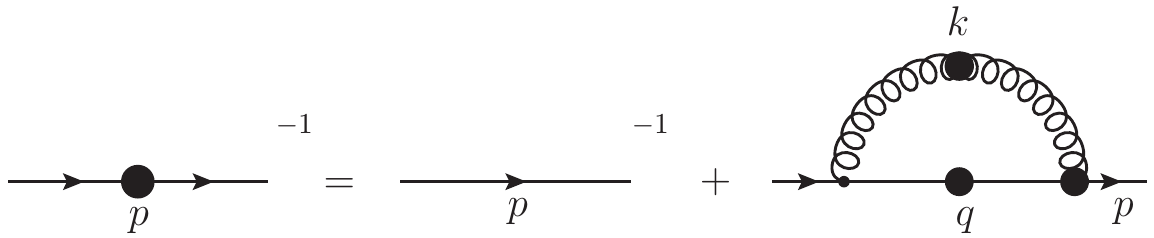
\includegraphics[width=0.95\textwidth]{figures/quark_DSE_gen.png}
 \end{center}
 \caption{\footnotesize Quark \DS equations, circles denote dressed propagators and vertexes.}\label{fig:quark_DSE_gen} 
\end{figure*}
The \Eq{\ref{dse:DSE_coord}} is the quark propagator in coordinate space. Multiplying with $S^{-1}(y-y^{\prime})$ , integrating over $y^\prime$ and performing the standard Fourier transformation gives the quark DSE in momentum space:
\beqa
	\label{dse:DSE_mom}
	S^{-1}(p) = (i\pslash - m) - ig^2\int \frac{d^4k}{(2\pi)^4} D^{\mu\nu}(k)\gamma_\mu S(q) \Gamma_\nu(p,q)\;.
\eeqa
So far we considered a single color structure, which obviously does not represent a full picture of the underlying physics. Thus we need to introduce the color structure into \Eq{\ref{dse:DSE_mom}}, by interchanging $\Gamma_\nu(p,q) \rightarrow  \Gamma^a_\nu(p,q)$, where $a=1,...,8$ denotes an index in $SU(3)$ adjoint representation, and also $\gamma_\mu \rightarrow \lambda^a \gamma_\mu$, where $\lambda^a$ are Gellmann matrices. Additionally the quark propagators carry implicitly the color index $i=1,2,3$, being the fundamental object of $SU(3)$ color group. Applying the aforementioned changes, we obtain the proper quark \DS equations:
\beqa
\label{dse:DSE_mom_full}
	S^{-1}(p) = (i\pslash - m) - ig^2\int \frac{d^4k}{(2\pi)^4} D^{\mu\nu}(k) \delta^{ab} \lambda^a \gamma_\mu S(q) \Gamma^b_\nu(p,q)\;.
\eeqa
This is integral equation is represented diagrammatically on Fig. \ref{fig:quark_DSE_gen}.
The full gluon propagator $D^{\mu\nu}(k)$ and full quark-gluon vertex $\Gamma_\nu(p,q)$ in \Eq{\ref{dse:DSE_mom_full}} satisfy their own DSEs, which connect them to higher n-point Green functions and by that create an infinite tower of equations. \\

However, this not final point of the derivation, since we have not yet defined the renormalization properties of the involved objects. The parameters like gauge coupling and quark mass are not physical and therefore should be expressed through experimental quantities. We achieve this by the multiplicative renormalization, which leads to the following replacements:
\beqa
	\label{dse:renorm}
\notag	&g=Z_g \tilde{g}\;, \;\;\; m = Z_m \tilde{m}\;, \\
	&S(p) = Z_2 \tilde{S}(p)\;, \;\; D^{\mu\nu}(k) = Z_3 \tilde D^{\mu\nu}(k)\;, \;\; \Gamma_\nu(p,q) = Z^{-1}_{1F} \tilde \Gamma_\nu(p,q)\;. \;\; \;\;\;\;\;\;
\eeqa
Here the $Z_{g,m,2,3,1F}$ are the renormalization factors for corresponding objects and tilde sign denotes the renormalized quantity. Note that this factors can be related to each other by universality of gauge coupling for any interaction vertices and due Slavnov-Taylor identity \cite{0201524724}. The following relations read as:
\beqa
	\label{dse:renorm_relations}
	&Z_g^{-1} = Z_3^{1/2} Z_2 Z^{-1}_{1F} = Z_3^{3/2} Z_1^{-1} = Z_3 Z_4^{-1/2} = Z_3^{1/2} \tilde Z_3 \tilde Z_1^{-1}\;, \\
	&\frac{Z_3}{Z_1} = \frac{Z_2}{Z_{1F}} = \frac{Z_3^{1/2}}{Z_4^{1/2}} = \frac{\tilde{Z_3}}{\tilde{Z_1}}\;,
\eeqa
where $Z_1, Z_4, \tilde{Z_3}, \tilde{Z_1}$ are the renormalization factors of the 3-gluon vertex, the 4-gluon vertex, the ghost propagator and the ghost-gluon vertex correspondingly. Using the aforementioned relations we can finally derive quark \DS equations for renormalized objects: 
\beqa
	\label{dse:DSE_full_renorm}
	S^{-1}(p) = Z_2(i\dslash - m) - ig^2Z_{1F}\int \frac{d^4}{(2\pi)^4} D^{\mu\nu}(k) \delta^{ab} \lambda^a \gamma_\mu S(q) \Gamma^b_\nu(p,q)\;,\;\;
\eeqa
suppressing a tilde notation for the renormalized quantities. Since gluon and quark propagators in Minkowski space can expose a non-analytical behaviour, for a purpose of numerical calculations we perform the Wick rotation \cite{PhysRev.96.1124} and throughout this thesis consider all our equations to be in Euclidean space-time. The detailed instruction how the Wick rotation is done is given in Appendix \ref{app:euclidean} \\

The Eq.(\ref{dse:DSE_full_renorm}) contains important pieces, which have to be specified. $D^{\mu\nu}(k)$ is the dressed gluon propagator, that satisfies its own DSE and in Euclidean space and Landau gauge have the following general form:
\beqa
	D^{\mu\nu}(k) = \frac{G(k^2)}{k^2}\left( \delta^{\mu\nu} - \frac{k^\mu k^\nu}{k^2} \right) \;,
\eeqa 
where $G(k^2)$ is gluon dressing function, connected to the gluon vacuum polarisation function via $G(k^2)=1/(1 + \Pi(k^2))$. 
The dressed quark-gluon vertex $\Gamma_\nu(p,q)$ also posses its own DSE with the solution in its general form given by 12 scalar functions. The Dirac basis is generated by linear combination of three Lorenz vectors $\{ \gamma^\mu \;, p^\mu \;, q^\mu \}$, each multiplied with one of the four Lorenz scalar matrices $\{ \ONE\;, \pslash \;, \qslash \;, \sigma^{\mu\nu}p_\mu q_\nu\}$. This choice is not unique, the basis is constrained only by Lorentz transformation properties. The explicit expression of general quark-gluon vertex is given by:
\beqa
\label{dse:gluon_vertex_gen}
	\Gamma_\mu(p,q) = \sum_{i=1}^{12}V^i(p,q) T^i_\mu(p,q) \;,
\eeqa
where $T^i_\mu(p,q)$ is employed Dirac basis and $V^i(p,q)$ are scalar dressing functions of the quark-gluon vertex. \\

The general form of the solution for Eq. \ref{dse:DSE_full_renorm} is full (dressed) quark propagator, given in terms of two scalar dressing functions and corresponding Dirac basis and in Euclidean space can be written as:
\beqa
	\label{dse:S_gen}
	S^{-1}(p) = i\pslash A(p^2,\mu^2) + B(p^2,\mu^2) = Z^{-1}(p^2,\mu^2)[i\pslash + M(p^2)]\;,
\eeqa
where $Z(p^2,\mu^2)$ and $M(p^2)$ are the quark wave function renormalization and the dressed mass function respectively. At this point we explicitly declared the renormalization point $\mu$ dependence of the dressing functions and introduced the $\mu^2$ - the renormalization scale. In order to address the renormalization procedure we need to unfold Eq. \ref{dse:DSE_full_renorm} by projecting out equations for each dressing function $A(p^2)$ and $B(p^2)$, using projectors $P_A=-i\frac{\pslash}{p^2}$ and $P_B=\ONE$ correspondingly: 
\beqa
\label{dse:DSE_AB}
	A(p^2) &=& Z_2(\mu) + Z_{1F}C_Fg^2\int\frac{d^4}{(2\pi)^4} D^{\mu\nu}(k)\Tr\left[ P_A \gamma_\mu S(q) \Gamma^b_\nu(p,q) \right]\; \;\;\;\;\; \\
\notag	B(p^2) &=& m_R(\mu) + Z_{1F}C_Fg^2\int\frac{d^4}{(2\pi)^4} D^{\mu\nu}(k)\Tr\left[ P_B \gamma_\mu S(q) \Gamma^b_\nu(p,q) \right]\;, \;\;\;\;\;
\eeqa
here $C_F=4/3$ is the Casimir operator for color $SU(3)$ and the trace is performed over Dirac indexes. The renomalization constants $Z_2$ and $m_R$ can be obtained by applying the following renomalization conditions:
\beqa
	\label{dse:renorm_cons}
	A(\mu^2,\mu^2) &=& 1 \\
	B(\mu^2, \mu^2) &=& m_R \;,
\eeqa
after which the equations for constants $Z_2$ and $m_R$ read as:
\beqa
	Z_2(\mu^2,\Lambda^2) &=& 1 - A(\mu^2,\Lambda^2) \\
	m_R(\mu^2) &=& Z_2(\mu^2,\Lambda^2)m_{bare} - B(\mu^2,\Lambda^2) \;,
\eeqa
where $\Lambda^2$ is numerical integration cut-off. \\

The Eq. (\ref{dse:DSE_AB}) is a final representation of quark \DS equation, which is of immense importance, being the main piece of the whole framework. The quark DSE itself allows to study the chiral symmetry breaking and dynamical quark mass generation. It is the crucial building block for \BS equation and Faddeev equations - the two-body and three-body bound state equations correspondingly, which are to be considered in Chapter \ref{chap:BSE}. 


\section{Truncation}
\subsubsection*{Rainbow-ladder ansatz}
\label{sec:RL}
The essential input to quark DSE is full(dressed) gluon propagator and full(dressed) quark-gluon vertex, given by their own \DS equations, which are forming, as it was mentioned, an infinite tower of equations, setting relations between higher order n-point Green functions. Therefore in order to be able to solve them, we need to apply a certain truncation or \textit{ansatz} for these correlation functions. As a first step in this work we will consider a so-called \textit{rainbow-ladder} truncation \cite{Maris:1997hd}, that on quark DSE level leads to the replacement:
\beqa
	\label{dse:RL_trunc}
Z_{1F} \frac{g^2}{4\pi} D_{\mu\nu}(q)\Gamma^\nu(k,p) \rightarrow Z_2^2T_{\mu\nu}(q) 
\frac{\alpha_{\mathrm{eff}}(q^2)}{q^2}\gamma^\nu\;,
\eeqa
here the $T_{\mu\nu}(q)=\delta_{\mu \nu}-\frac{q_\mu q_\nu}{q^2}$ is the transverse projector and the $\alpha_{\mathrm{eff}}(q^2)$ is effective running coupling. This is the simplest \textit{ansatz} satisfying the axial Ward-Takahashi identity (axWTI), as we will discuss in Chapter \ref{chap:BSE}, and essentially takes into account only the $\gamma_\mu$-structure of the dressed quark-vertex and combines all dressing effects of the gluon and the vertex into an effective running coupling $\alpha_{\mathrm{eff}}(q^2)$ . The resulting diagram expression for quark \DS equations is given on Fig. \ref{fig:DSE_RL}.
\begin{figure}[H]
\tiny
 \begin{center}
  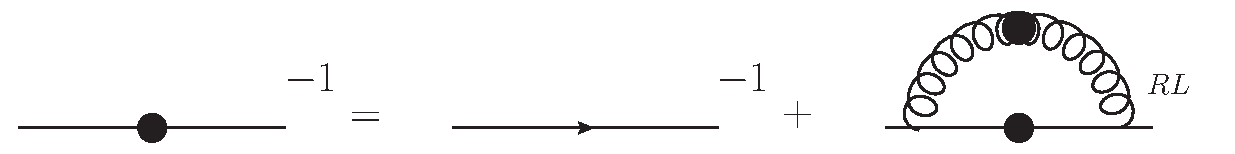
\includegraphics[width=0.95\textwidth]{figures/DSE_RL}
 \end{center}
 \caption{\footnotesize The quark \DS equations, within RL truncation. Lines with filled circles note fully dressed propagators.  }\label{fig:DSE_RL} 
\end{figure}
However, as we will show later, this truncation is very useful as a first exploratory step toward the reverse engineering of QCD at low energies. The resulting expression for the quark \DS equation reads as:
\beqa
\displaystyle S^{-1}(p)=Z_2 S^{-1}_0(p) + C_F (Z_2)^2 \int \frac{d^4 k}{(2\pi)^4} \gamma_{\mu} S(k) \gamma_{\nu} T_{\mu\nu}(q) \frac{4\pi\alpha_{\mathrm{eff}}(q^2)}{q^2}\;,
\label{dse:DSE_RL}
\eeqa
where $C_F=(N_c^2-1)/2N_c$ is the Casimir operator coming from the color trace. \\

The choice of $\alpha_{\mathrm{eff}}$ is dictated from one side by the phenomenologically
required infrared enhancement of the effective single gluon interaction, necessary for the dynamical 
generation of a constituent-like quark mass and a chiral vacuum quark condensate. From another side its ultraviolet behaviour has to match to the perturbative one and therefore ensure the preservation of one-loop results. As a model for $\alpha_{\mathrm{eff}}(q^2)$ that takes into account aforementioned criteria we take that of Maris and Tandy \cite{Maris:1999nt}, which explicit expression reads as following:
\beqa
\label{dse:MT_model}
\alpha_{\mathrm{eff}}(q^2)=\pi\eta^7x^2e^{-\eta^2x}
+\frac{2\pi\gamma_m\left(1-e^{-y}\right)}{\log\left[e^2-1+(1+z)^2\right]}\;,
\eeqa
where $x=q^2/\Lambda^2$, $y=q^2/\Lambda_t^2$, $z=q^2/\Lambda_{\mathrm{QCD}}^2$. 
Here $\Lambda_t=1$~GeV is a regularization parameter for the perturbative logarithm;
its value has no material impact on the numerical results. The QCD-scale 
$\Lambda_{\mathrm{QCD}}=0.234$~GeV controls the running of the logarithm with
anomalous dimension $\gamma_m=12/25$ corresponding to four active quark flavors.
The infrared strength of this model is controlled by the parameters $\Lambda$ and 
$\eta$. While $\Lambda = 0.72$ GeV is fixed from the pion decay constant, there is considerable
freedom to vary the dimensionless parameter $\eta$. The explicit view of this interaction model, with provided parameters, is given on Fig. \ref{fig:MT_graph}. 
\begin{figure*}[t]
\tiny
 \begin{center}
  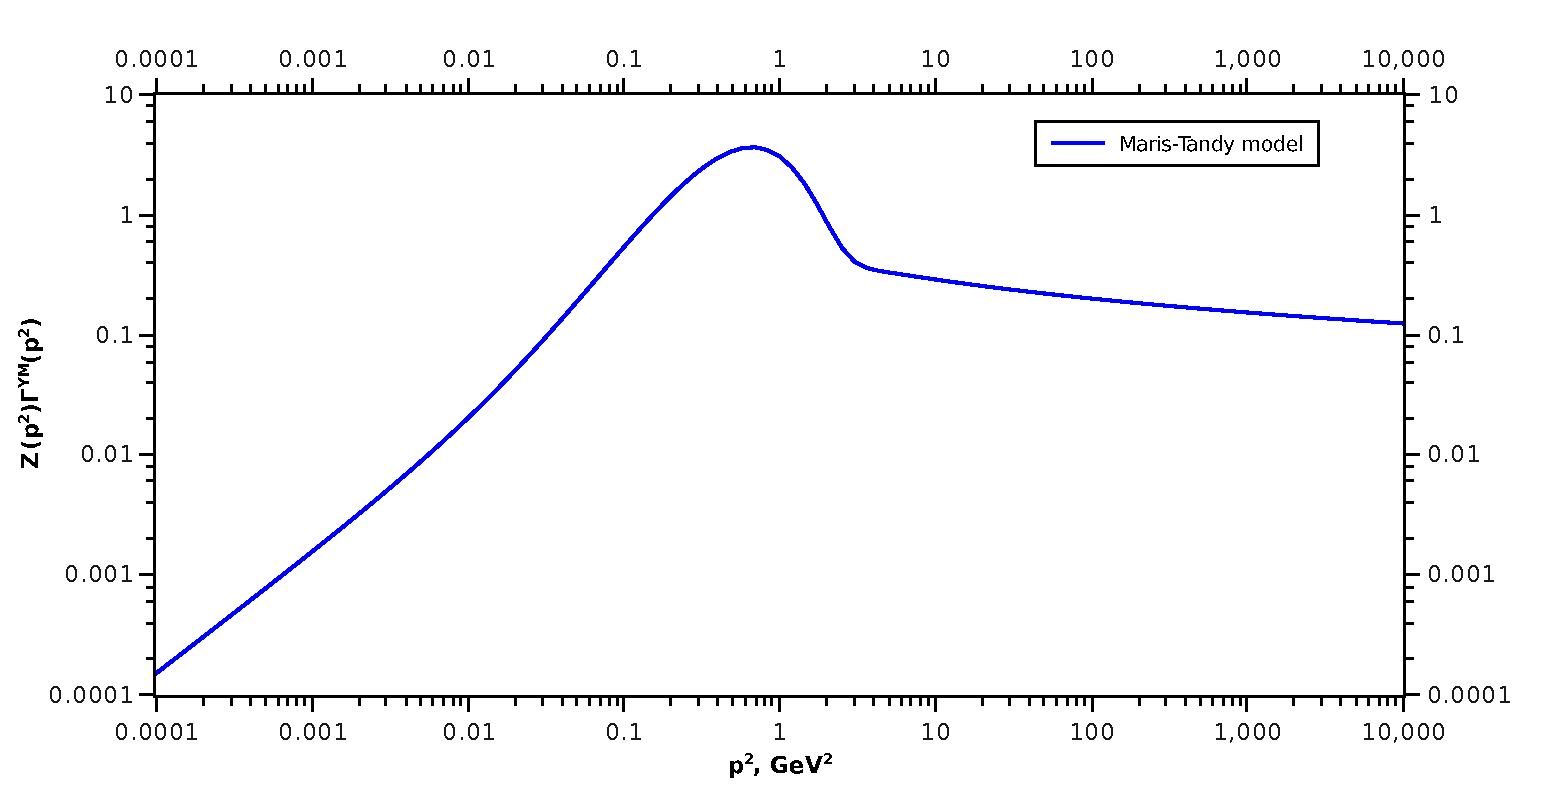
\includegraphics[width=0.95\textwidth]{figures/Gluon_MT_graph}
 \end{center}
 \caption{\footnotesize Gluon dressing function $\frac{\alpha_{\mathrm{eff}}(q^2)}{q^2}$ in Maris--Tandy model \cite{Maris:1999nt}. The $\Lambda = 0.72$ GeV and $\eta = 1.8$ GeV }\label{fig:MT_graph} 
\end{figure*} \\

Despite the apparent simplicity of the gluon model and the truncation employed, this approach can successfully describe: light pseudoscalar and vector masses and decay constants\cite{Maris:1997tm, Maris:1999nt}, $\pi$, $K^+$, $K^0$ electromagnetic form factors\cite{Maris:2000sk}, $\gamma \pi \gamma$-transition\cite{Maris:2002mz}, strong decays\cite{Jarecke:2002xd}. In the course of this work the same approach with a few technical adjustments was used to describe the spectra of light and heavy mesons and to make a prediction for $J^{PC}=3^{--}$ for charmonium and bottomonium bound states \cite{Fischer:2014cfa, Fischer:2014xha}. This results are represented in Chapter \ref{chap:spectra}.
%
%
%
\subsubsection*{Unquenching effect}
However the \DS equations framework is not bounded to aforementioned truncation. Over the years were made a huge amount of successful efforts to go beyond Rainbow-Ladder approach. One of promising routes is to use explicit diagrammatic approximations to the DSE of the quark-gluon vertex \cite{Bender:1996bb,Watson:2004kd,Bhagwat:2004hn,Matevosyan:2006bk,Alkofer:2008tt,Fischer:2007ze,Fischer:2009jm}. 
\begin{figure}[H]
\tiny
 \begin{center}
  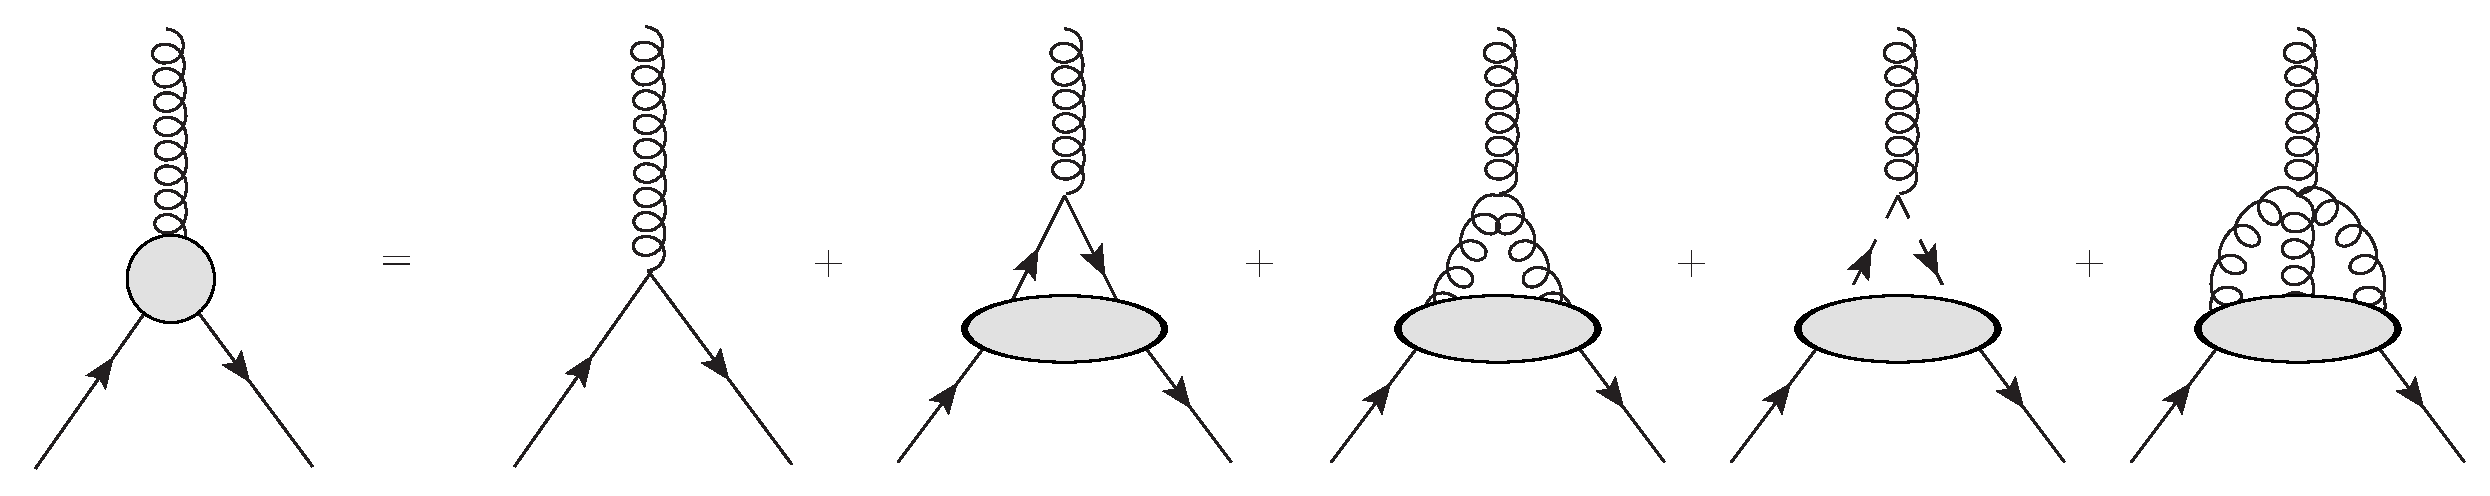
\includegraphics[width=0.95\textwidth]{figures/qqg_vertex_gen}
 \end{center}
 \caption{\footnotesize The full, untruncated \DSE for the quark-gluon vertex. }\label{fig:qqg_vertex_gen} 
\end{figure}
The the full, untruncated \DSE for the quark-gluon vertex is given diagrammatically in
Fig. \ref{fig:qqg_vertex_gen}. Here we are primarily interested in the mid-momentum behavior of the vertex and in particular in hadronic
contributions. To lowest order in a skeleton expansion such contributions can only occur in the diagram with the bare quark-gluon vertex at the external gluon line. 
\begin{figure}[H]
\tiny
 \begin{center}
  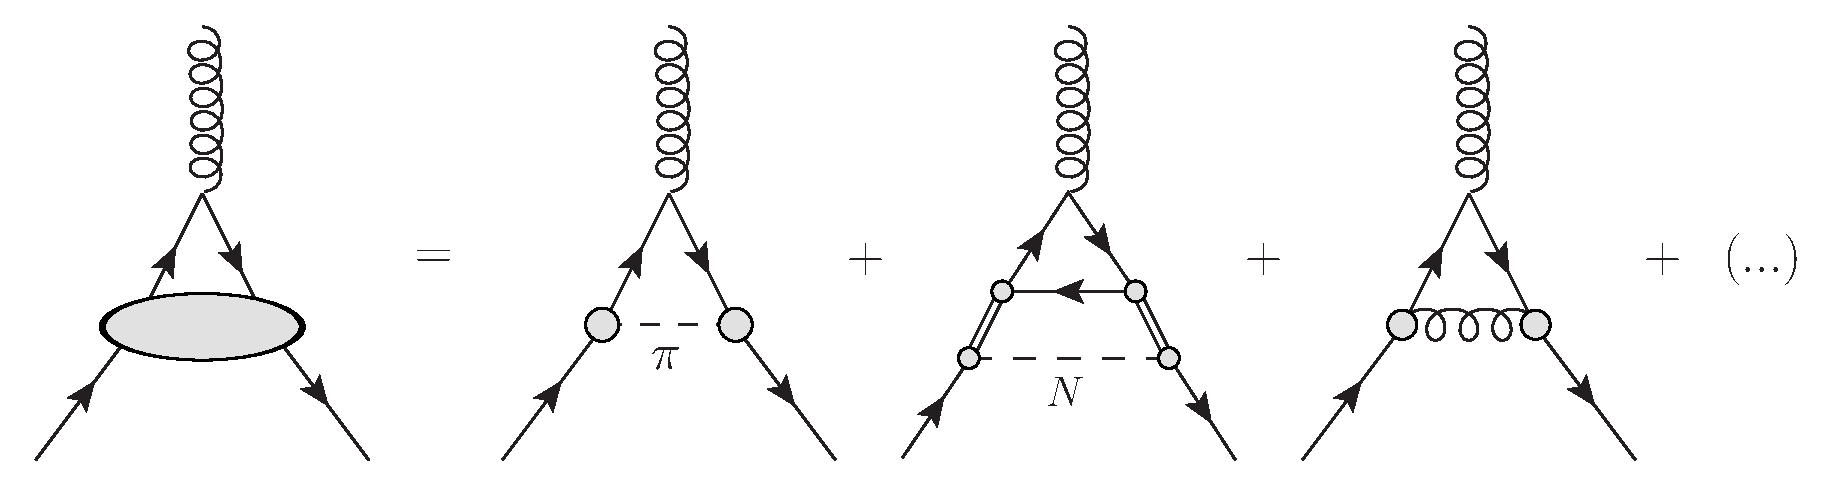
\includegraphics[width=0.95\textwidth]{figures/qqg_hadron}
 \end{center}
 \caption{\footnotesize The expansion in terms of hadronic and non-hadronic
contributions to the quark-antiquark scattering kernel. The dotted line describes mesons, the dashed line baryons and the double lines correspond to diquarks.  }\label{fig:qqg_hadron} 
\end{figure}
Consider this diagram that consists of quark-antiquark scattering kernel, which can be expanded in terms of one-particle irreducible Green's functions and resonance exchange contributions, as it is given on Fig. \ref{fig:qqg_hadron}. Of all those the term containing the pion one-meson exchange should be dominant, since further diagrams with exchange of heavy mesons and baryons, $(K, \rho, N, ...)$, are suppressed by their masses accordingly. 
This approximation allows to study the pion cloud effects on the spectrum of light mesons \cite{Fischer:2007ze,Fischer:2008sp,Fischer:2008wy} and 
baryons \cite{Sanchis-Alepuz:2014wea}. Also it is beneficial to have explicit hadronic degrees of freedom, since the pion cloud effects 
are expected to play an important role in the low momentum behaviour of form factors and hadronic decay processes of baryons
\cite{Thomas:1981vc,Miller:2002ig,Ramalho:2008dp,Cloet:2012cy,Eichmann:2011vu, Eichmann:2011aa,Sanchis-Alepuz:2013iia}. It should be noted, however, pions are not elementary fields and their wave functions must to be determined from their Bethe-Salpeter equation, as we will see in Chapter 4. \\

On another hand, the infrared domain of the quark propagator and its analytic structure heavily depends on the quark-gluon vertex truncations, such that, in principle all twelve Dirac structures from Eq. (\ref{dse:gluon_vertex_gen}) can be important \cite{Skullerud:2003qu,Kizilersu:2006et}. Therefore it is crucial to  utilise explicit notations for tensor structures of quark-gluon vertex beyond the leading $\gamma_\mu$ term \cite{Chang:2009zb,Chang:2010hb,Chang:2011ei,Heupel:2014ina,Williams:2014iea}. \\ 

In the course of this work we will incorporate into the coupled system of \DS and \BS equations the pion cloud effect, provided by scheme \cite{Fischer:2008wy}, where was obtained the good agreement with lattice QCD and meson phenomenology. Since this effect is generated due to the presence of dynamical sea quarks, it can be considered as unquenching effect. In this case the truncation take following form:
\beqa
	\label{dse:RL_pi_truncation}
Z_{1F} \frac{g^2}{4\pi} D_{\mu\nu}(q)\Gamma^\nu(k,p) \rightarrow Z_2^2T_{\mu\nu}(q) 
\frac{\alpha_{\mathrm{eff}}(q^2)}{q^2}\gamma^\nu -\frac{1}{C_F}\tau^iZ_2\gamma_5\Gamma_\pi ( \frac{p+k}{2};q )\;,
\eeqa
where $\tau^i$ are $SU(2)$ isospin symmetry generators and $\Gamma_\pi (\frac{p+k}{2};q)$ is the full pion wave function, evaluated at symmetrized momenta and given by 4 Dirac components:
\beqa
	\Gamma_\pi (p;P) = \gamma_5 \left[  E(p;P)\ONE + F(p;P)\Pslash + G(p;P)\pslash + H(p;P)\sigma^{\mu\nu}p_\mu P_\nu \right] 
	\label{dse:pion_vertex_gen}
\eeqa
On diagrammatical level this leads to addition of an extra diagram involving the pion exchange and pion wave function, as it is represented by Fig. \ref{fig:DSE_PS}.
\begin{figure}
\tiny
 \begin{center}
  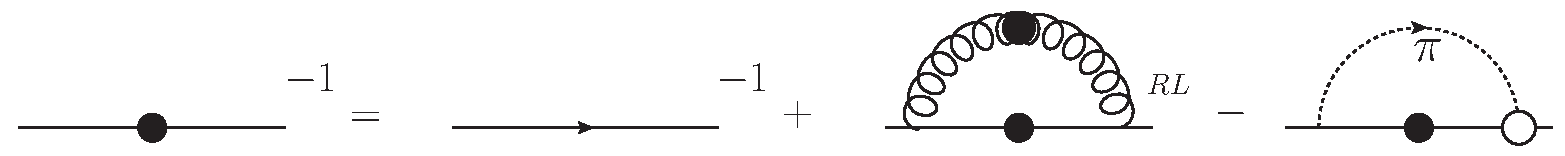
\includegraphics[width=0.95\textwidth]{figures/DSE_with_pi}
 \end{center}
 \caption{\footnotesize The quark \DS equations, within Rainbow-Ladder truncation with unquenching pion cloud effect. Lines with filled circles note fully dressed propagators.  }\label{fig:DSE_PS} 
\end{figure}
The explicit form of corresponding quark DSE can be written as following:
\beqa
\displaystyle S^{-1}(p)=Z_2 S^{-1}_0(p) + C_F (Z_2)^2 \int \frac{d^4 k}{(2\pi)^4} \gamma_{\mu} S(k) \gamma_{\nu} T_{\mu\nu}(q) \frac{4\pi\alpha_{\mathrm{eff}}(q^2)}{q^2} \;\;\;\;\;\;\;\;\; \\
\notag - 3 \, Z_2 \int \frac{d^4 k}{(2\pi)^4} \left[\gamma_5 S(k) \Gamma_\pi ( \frac{p+k}{2};k-p ) + \gamma_5 S(k) \Gamma_\pi ( \frac{p+k}{2};p-k ) \right] \frac{D_\pi(q^2)}{2}
\label{dse:DSE_PS}
\eeqa
Where $q=p-k$, the quark renormalization constant $Z_2$, the fully dressed inverse quark propagator $S^{-1}(p)=i \slashed p A(p^2) + B(p^2)$, inverse bare one $S^{-1}_0(p)=i \slashed p  + m$ and $D_\pi(q^2)=\frac{1}{q^2+M^2_\pi}$.  
The first line is the Rainbow-Ladder contribution, where the same modelling was applied as in \ref{sec:RL}. The second line embodies the pion cloud effect, that satisfies the axial-vector Ward-Takahashi(AxWTI) identity, with the vertex $\Gamma_\pi (p;P)$ being the full pion wave function. Here, the coupling of the pion to the quark is given by a bare pseudoscalar vertex and a full pion Bethe-Salpeter amplitude. Note, however, that in general also the choice of two dressed vertices is possible and it is not clear a priori, which of the two choices is the better approximation of the original two-loop diagram. In \cite{Fischer:2008wy} the choice with one bare vertex led to satisfactory results in the vector-meson sector and we will therefore adopt this also here. \\

For a reasons of numerical simplicity we employ the approximation to the full pion Bethe-Salpeter wave function by the
leading amplitude $E(p;P)$ in the chiral limit, which is due to AxWTI given by \cite{Maris:1997hd}:
\beqa
	\Gamma_\pi(p;P) =\gamma_5 E(p;P) = \gamma_5 \frac{B(p^2)}{f_\pi}\;,
	\label{dse:pion_vertex}
\eeqa
where $B(p^2)$ is the scalar dressing function of the inverse quark propagator, taken in the chiral limit $m_q \rightarrow 0$. The $f_\pi = 93 \; \text{MeV}$ is the pion weak decay constant. This approximation omits the back-coupling effects of the three sub-leading amplitudes. Note however, this approximation is only strictly valid in chiral limit and approximately valid at physical pion mass point. For the high pion mass calculation carried out throughout this thesis we employed explicitly calculated first pion amplitude $E(p;P)$ in rainbow-ladder approach, continued into complex relative momentum $p$ via the same continuation procedure we used for the quark propagator, which is described in Appendix \ref{app:numerics}. As it was shown in Ref. \cite{Fischer:2008sp}, where full back-coupling has been evaluated in a real value approximation, the omission of $F(p;P), G(p;P), H(p;P)$ pion amplitudes leads to an error of only a few percent for meson masses and of about 10-20\% for decay constants for a physical pion. Note that we use aforementioned approximation only for the internal pion wave function, as it sets the interaction. The biggest advantage of the approximation Eq. (\ref{dse:pion_vertex}) compared to the full back-coupling performed in Ref. \cite{Fischer:2008sp} is that the Eq. (\ref{dse:DSE_PS}) can be solved self-consistently without any external input from pion \BS equation, so that it reduces the numerical efforts dramatically. \\

%
\section{Numerical solution of the DSE}
In this section we will demonstrate the numerical solutions of the Eq. \ref{dse:DSE_RL} and \ref{dse:DSE_PS}. Clearly the polarization tensor of the resulting dressed propagator must have the following form: $S(p) =i \sigma_v(p^2) \pslash + \sigma_s(p^2)$ and for inversed $S^{-1}(p)=-i A(p^2)\pslash + B(p^2)$, with $\sigma_v = \frac{A}{A^2 p^2 + B^2}$ and $\sigma_s = \frac{B}{A^2 p^2 + B^2}$. These unknown dressing functions $A(p^2)$ and $B(p^2)$ are the solution of quark \DS equations, which we intent to find. Throughout this work we apply the iteration method to solve the quark \DS equations, which appear to be nonlinear integral equations, and obtain aforementioned dressing functions. We put a more detailed description of this numerical procedure into Appendix \ref{app:numerics}. \\

At first we consider the Euclidean space solutions of quark DSE obtained within \textit{rainbow-ladder} truncation Eq. (\ref{dse:RL_trunc}), since the solving procedure does not require special treatment of the integration momenta as for the pion exchange. The resulting quark wave function $Z(p^2)$ and quark mass function $M(p^2)$ are shown on Fig. \ref{fig:quark_Z_func} and Fig. \ref{fig:quark_M_func} correspondingly. Note the gluon Maris-Tandy model parameters Eq. (\ref{dse:MT_model}) employed in this calculations are $\Lambda=0.72$ and $\eta=1.8$. The used renormalized current quark masses parameters for different flavor and type of quarks are of the same order as current quark masses in perturbative QCD and are given on Table. \ref{tab:mass_bare}. Note that we are consider the isosymmetric case, so the $m_{up}=m_{down}$.
\begin{table}[!h]
\renewcommand{\arraystretch}{1.3}
\begin{tabular*}{\columnwidth}{@{\extracolsep{\stretch{1}}}c|c|c|c|c|c@{}}
\hline
\hline
 & chiral & up/down & strange & charm & bottom \\
\hline
$m_{R} \; [GeV]$  & 0 & 0.0037 & 0.085 & 0.87 & 3.79 \\
\hline
\hline
\end{tabular*}
\caption{The values $m_{R}$ of used current quark mass parameters.  \label{tab:mass_bare}}
\end{table}
The renormalization point set to be $\mu=19\;\text{GeV}$. Aforementioned parameters are chosen to reproduce experimental masses of pion and rho mesons, $m_\pi, \; m_\rho$ and pion weak decay constant $f_\pi$, obtained via \BS equations as we will see in Chapter\;5 and are given in Table. \ref{tab:RL_params}.  \\
\begin{table*}
\centering
\renewcommand{\arraystretch}{1.3}
\begin{tabular}{c|c|c||c|}
\hline
\hline
          				     & \multicolumn{2}{c||}{RL1} & RL2 + pion cloud  \\
\hline
          				     & Light quark (u,d,s) & Heavy quarks (c,b) & Light quark (u,d,s) \\
 $\Lambda$ &  0.72    & 0.72 & 0.84 \\
$\eta$ & $1.8\pm 0.2$ & $1.257\pm 0.2$ & $1.8\pm 0.2$ \\                                                                                                                                                               
\hline
\hline
\end{tabular}
\caption{\footnotesize The values of effective single gluon model parameters.}\label{tab:RL_params}
\end{table*}
%
\begin{figure}
\tiny
 \begin{center}
  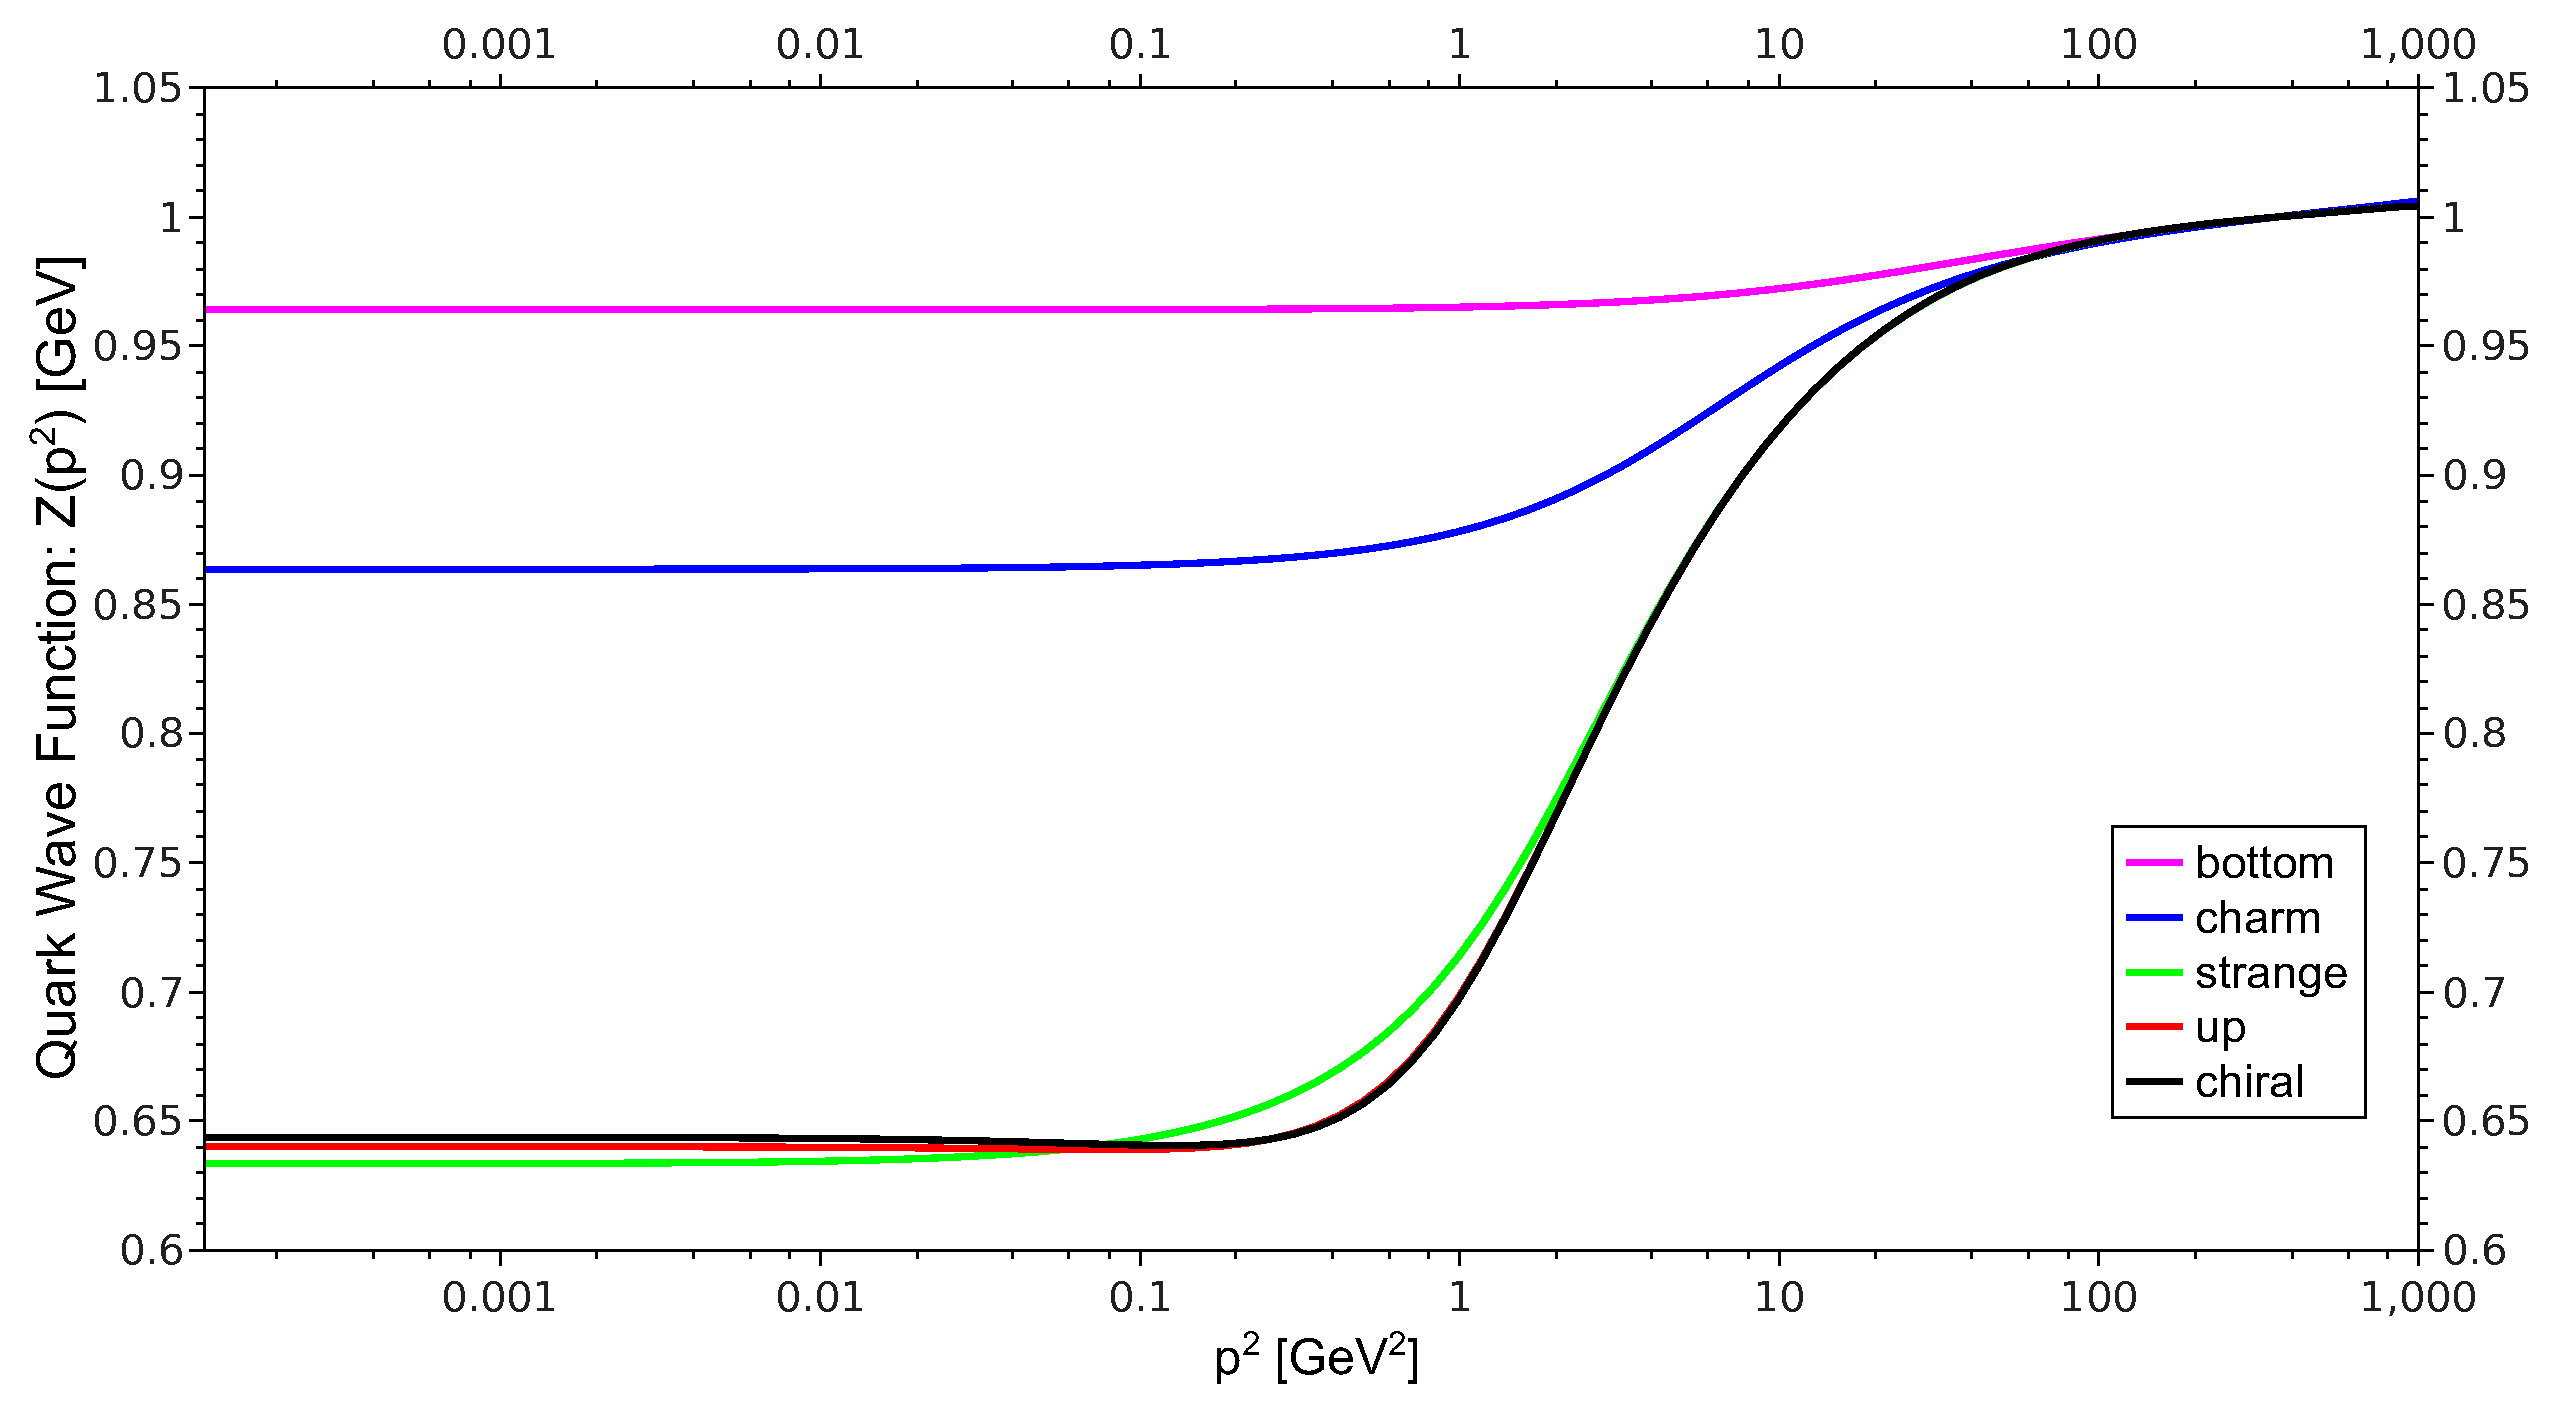
\includegraphics[width=0.95\textwidth]{figures/quark_Z_functions}
 \end{center}
 \caption{\footnotesize $Z(p^2)$ quark wave function renormalization for different types of quarks. The renormalizization point set to be $\mu=19\;\text{GeV}$. }\label{fig:quark_Z_func} 
\end{figure}

\begin{figure}
\tiny
 \begin{center}
  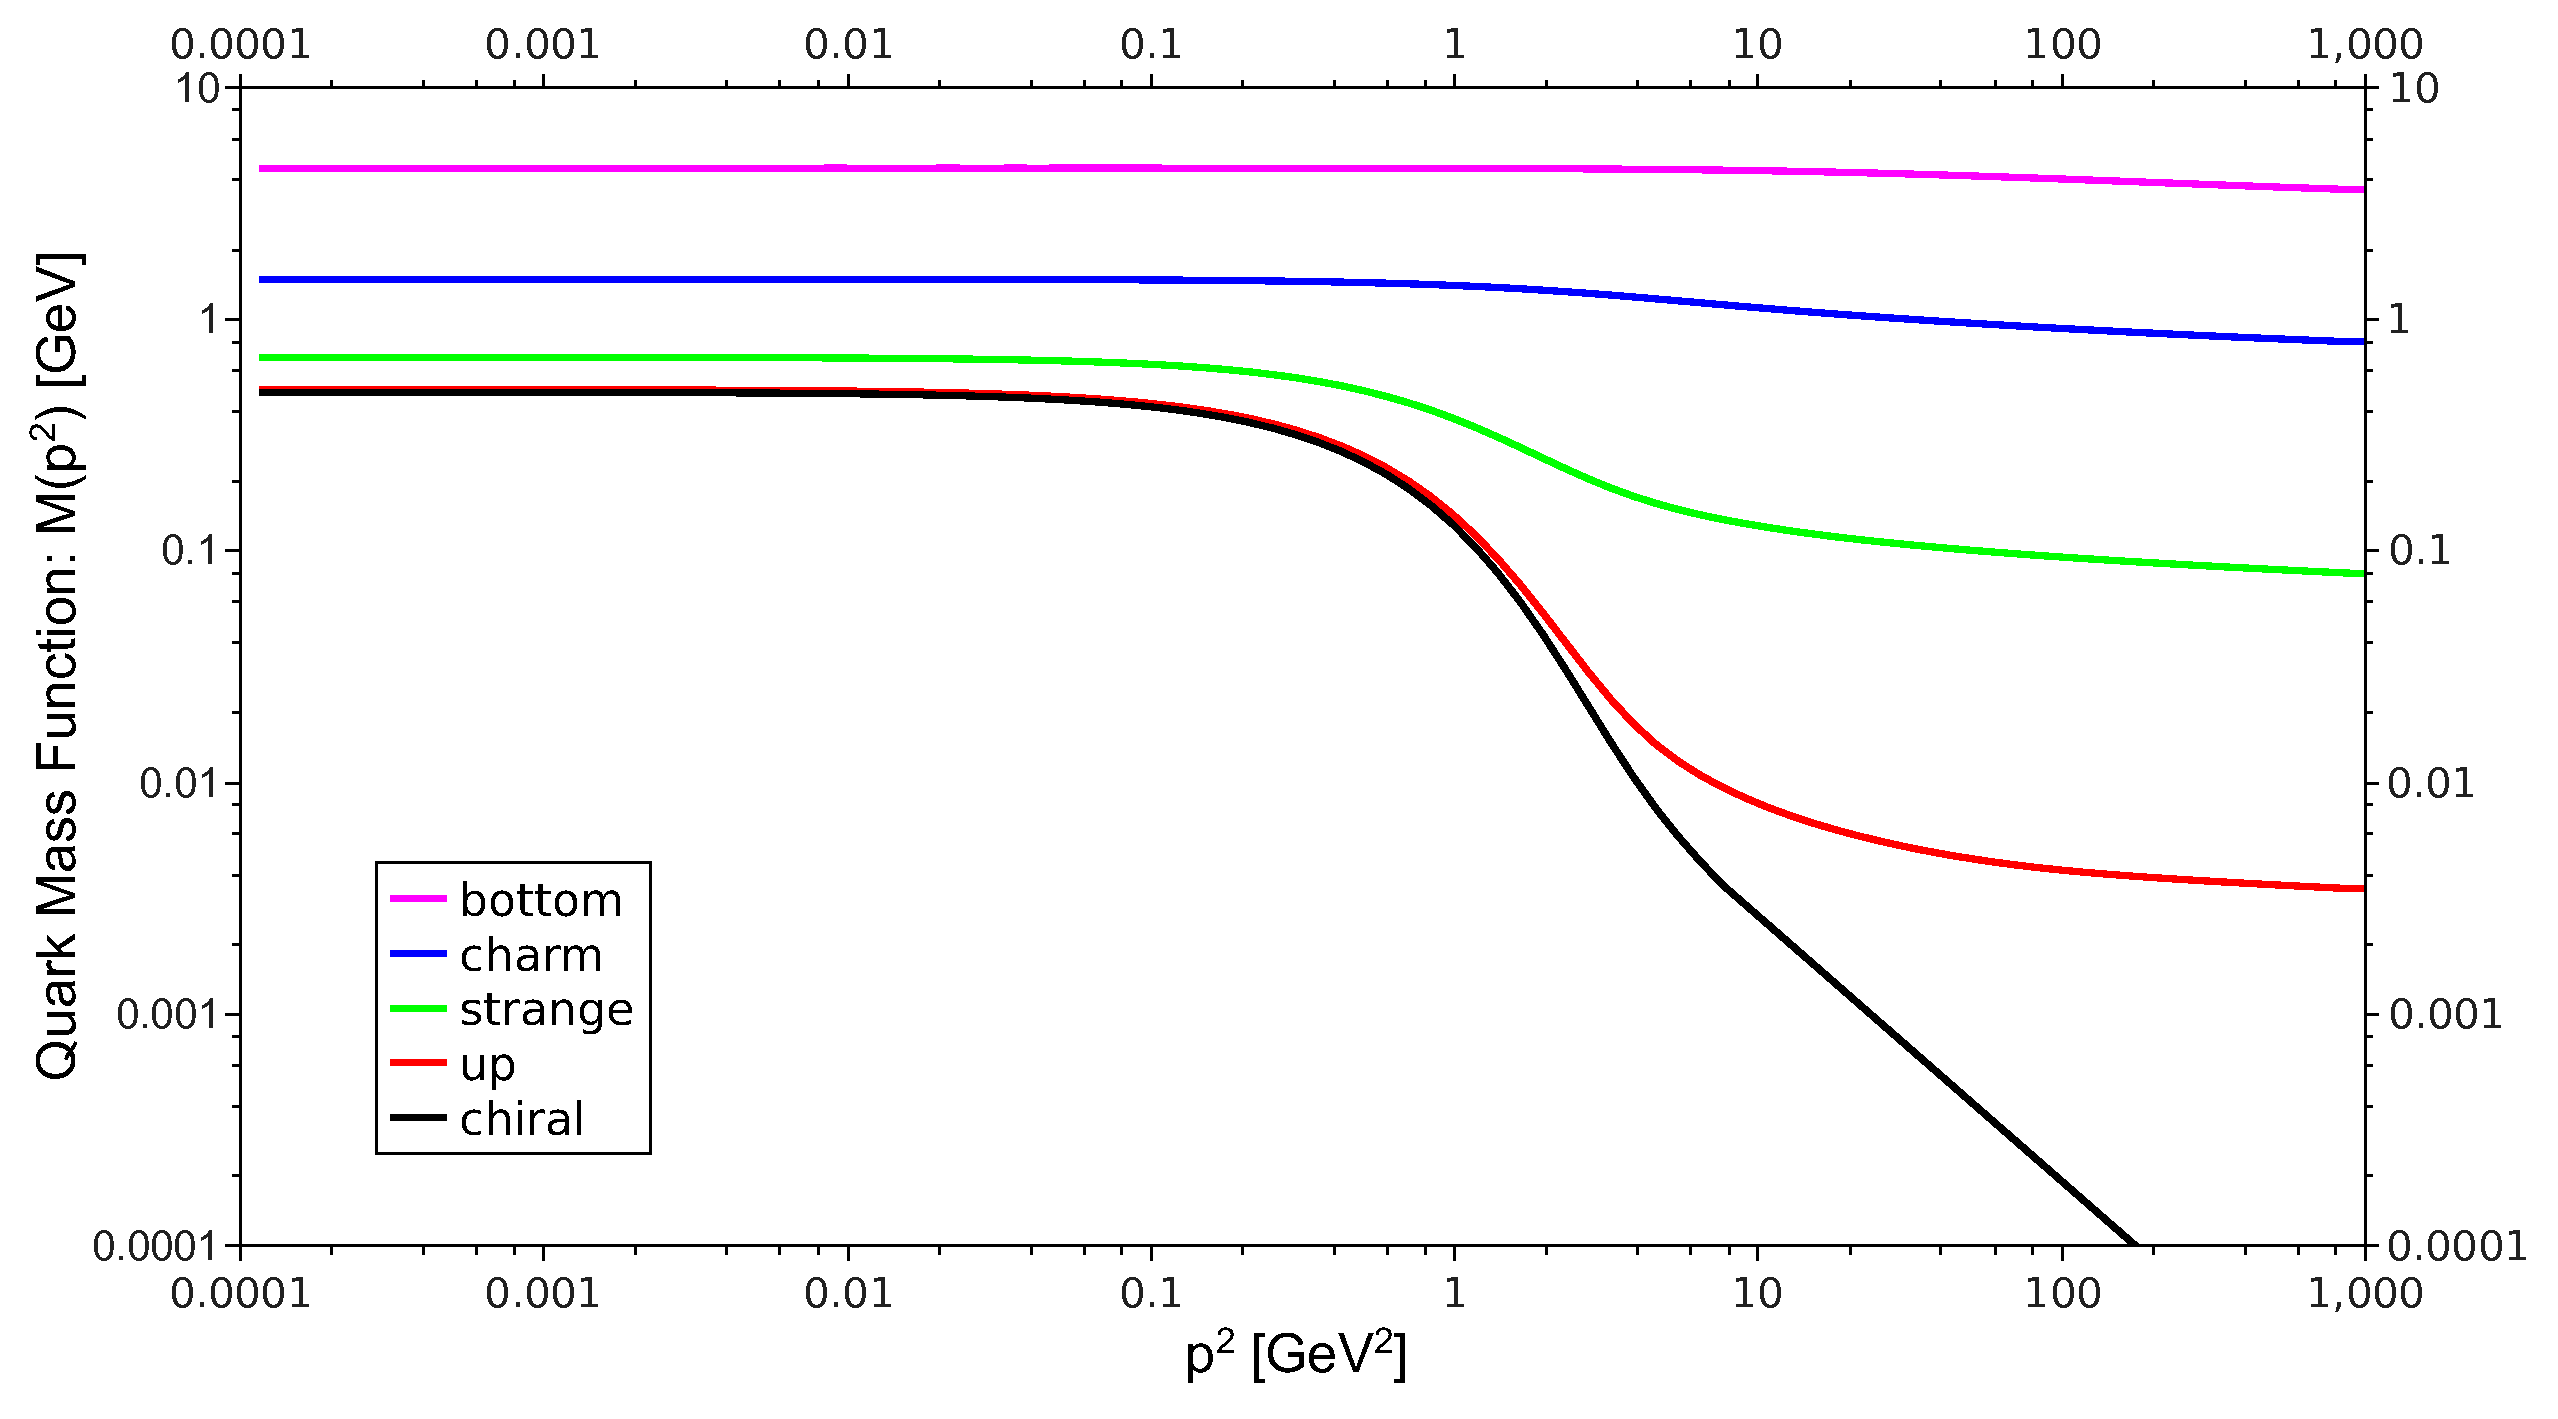
\includegraphics[width=0.95\textwidth]{figures/quark_M_functions}
 \end{center}
 \caption{\footnotesize $M(p^2)$ quark mass function for different types of quarks. The renormalizization point set to be $\mu=19\;\text{GeV}$. }\label{fig:quark_M_func} 
\end{figure}
The Fig. \ref{fig:quark_M_func} makes apparent that dynamical chiral symmetry (D$\chi$SB) is realized, i.e. in the rainbow-ladder truncation in a form Eq. (\ref{dse:RL_trunc}) with effective coupling given by Eq. (\ref{dse:MT_model}) the D$\chi$SB can provided. As we see in deep ultraviolet region the magnitude of $M(p^2)$ quark mass function is driven by renormalized quark mass, according to \cite{Miransky:1986ib}. It is logarithmicaly scaling down in a presence of explicit chiral breaking, i.e. non-zero bare quark mass $m_{bare}\neq 0$, as:
\beqa
	M(p^2) \approx \frac{1}{[\text{ln}(p^2/\Lambda^2_{QCD})]^{1/2\pi^2b}}
\eeqa
and in chiral case it is falling as $\mathbf{O}(1/p^2)$:
\beqa
	M(p^2) \approx \frac{1}{p^2}[\text{ln}(p^2/\Lambda^2_{QCD})]^{1/2\pi^2b-1}\;,
\eeqa
exposing irregular and regular behaviour respectively. In the infrared domain, however, the quark mass function enhances dramatically by orders of magnitude in comparison to current masses, especially for light quarks and chiral case. This enhancement is a clear evidence of dynamical mass generation from current quark mass to a constituent quark mass. Also this effect takes place at scale approximately $1\; \text{GeV}^2$, as it is meant to occur due to hadron phenomenology. Nevertheless, as will be shown in Chapter 5, the dynamically generated mass function in the chiral case used as input to pion \BS equations lead to zero pion mass $m_\pi=0$, fulfilling Gell-Mann--Oakes--Renner relation Eq. (\ref{qcd_low:GMOR}). \\ 
 \begin{figure*}[t]
 \begin{center}
  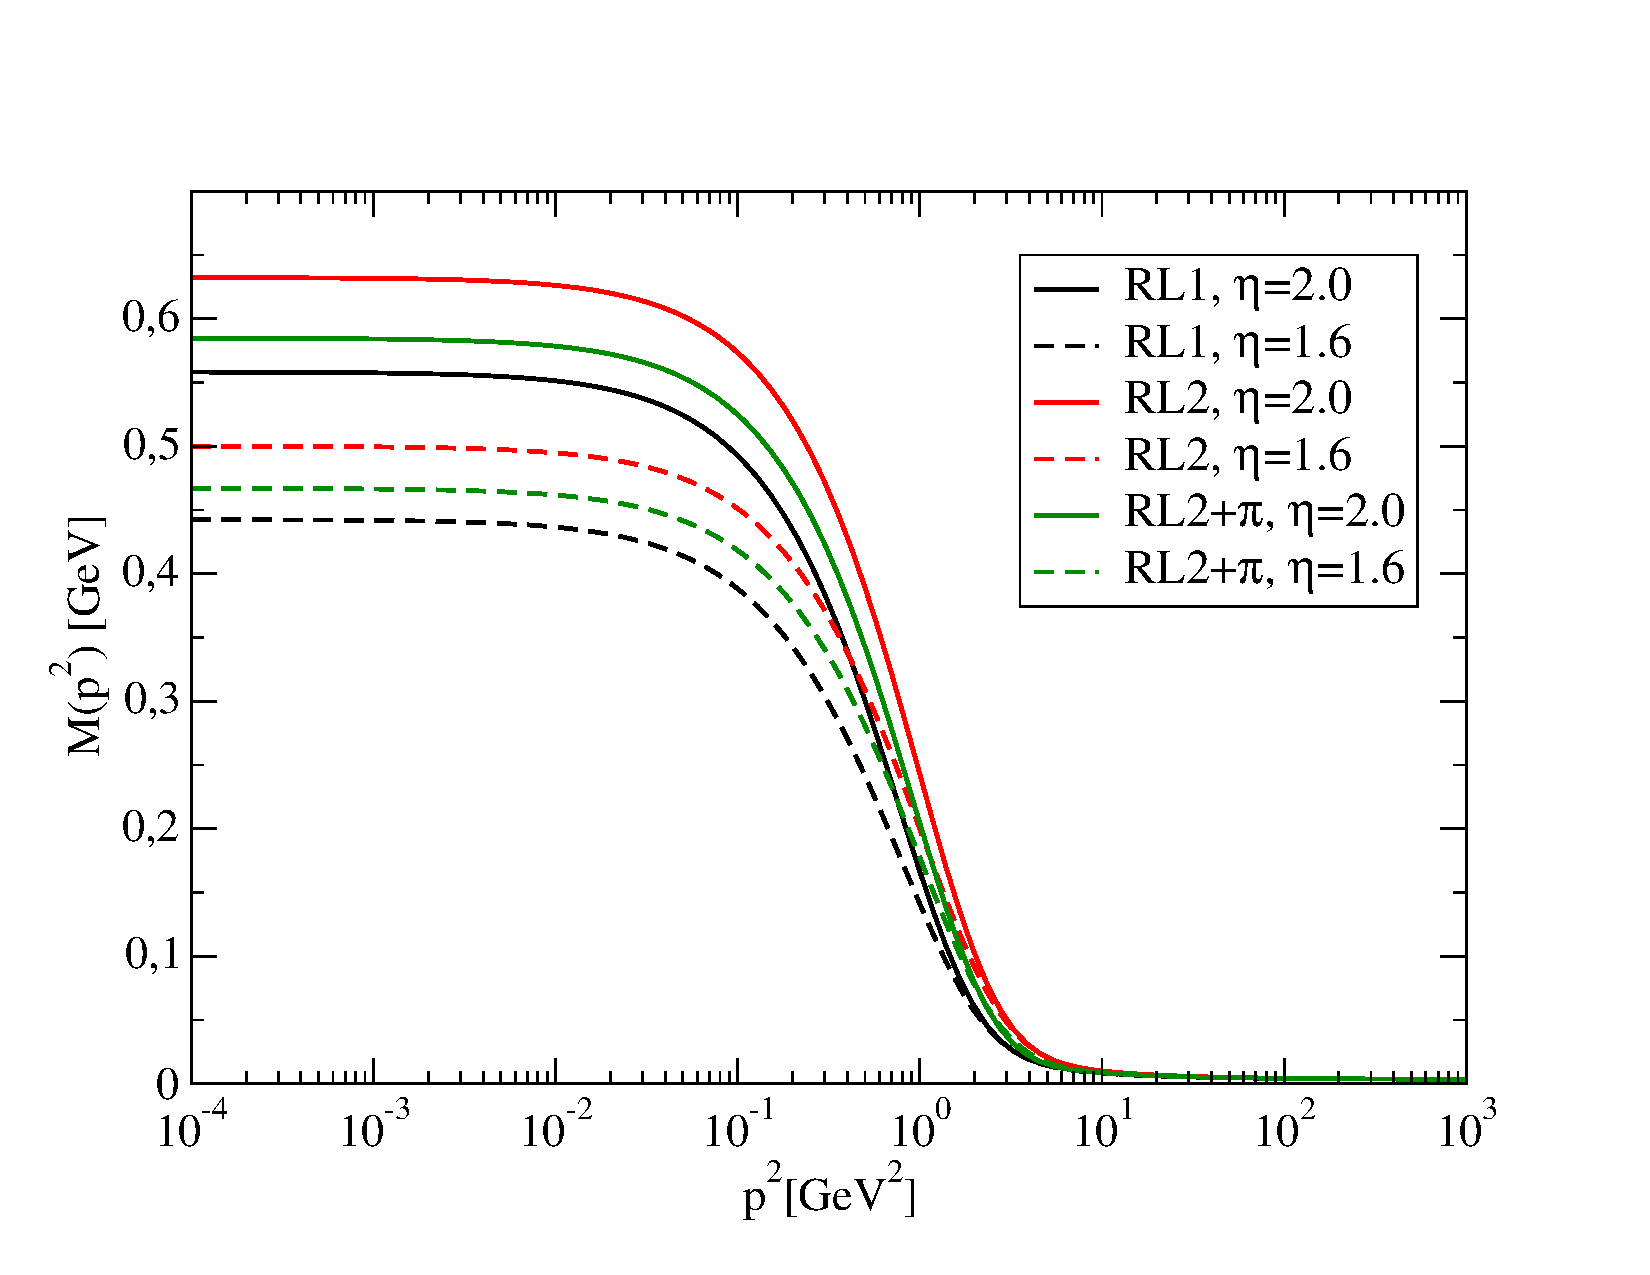
\includegraphics[width=0.95\textwidth,clip]{figures/mass}
 \end{center}
 \caption{$M(p^2)$ Quark mass function as function of the squared momentum.}\label{fig:RL_vs_PS}
\end{figure*}
In case of included pion cloud effect it requires extra numerical efforts to obtain the solutions. Similarly, the parameters $\Lambda$ and $\eta$ were fitted in order to reproduce experimental value of pion mass and pion decay constant, although the current mass of the up quark was kept the same. The new set of parameters are $\Lambda=0.84$ and $\eta=1.8$. The $\Lambda$ is increased to reflect the increased interaction range due to the added pion exchange. The resulting quark mass functions are displayed in Fig.~\ref{fig:RL_vs_PS}. For the 
two setups fixed by physical input, RL1 and RL2+$\pi$ given in Table \ref{tab:RL_params},
we find very similar mass functions with a difference in $M(0)$ of less than 
five percent. The quark-core setup $RL2$ generates slightly larger quark masses.
In general, the quark mass function encodes dynamical chiral symmetry breaking and 
nicely displays the transition from the low momentum notion of a constituent quark 
mass to the high momentum notion of a running current quark mass. Although the 
quark mass function is a renormalisation group invariant it is not, however, a 
gauge invariant quantity and therefore not directly observable. The chiral properties 
of our framework are also encoded in the dependence of the pion mass from the 
current quark mass. Further in Chapter \ref{chap:spectra} we explicitly checked the Gell-Mann-Oakes-Renner relation
for all setups and find that it holds within the numerical accuracy of 2 \%, 
as expected from the axWTI. 
\begin{figure}[h]
\tiny
 \begin{center}
  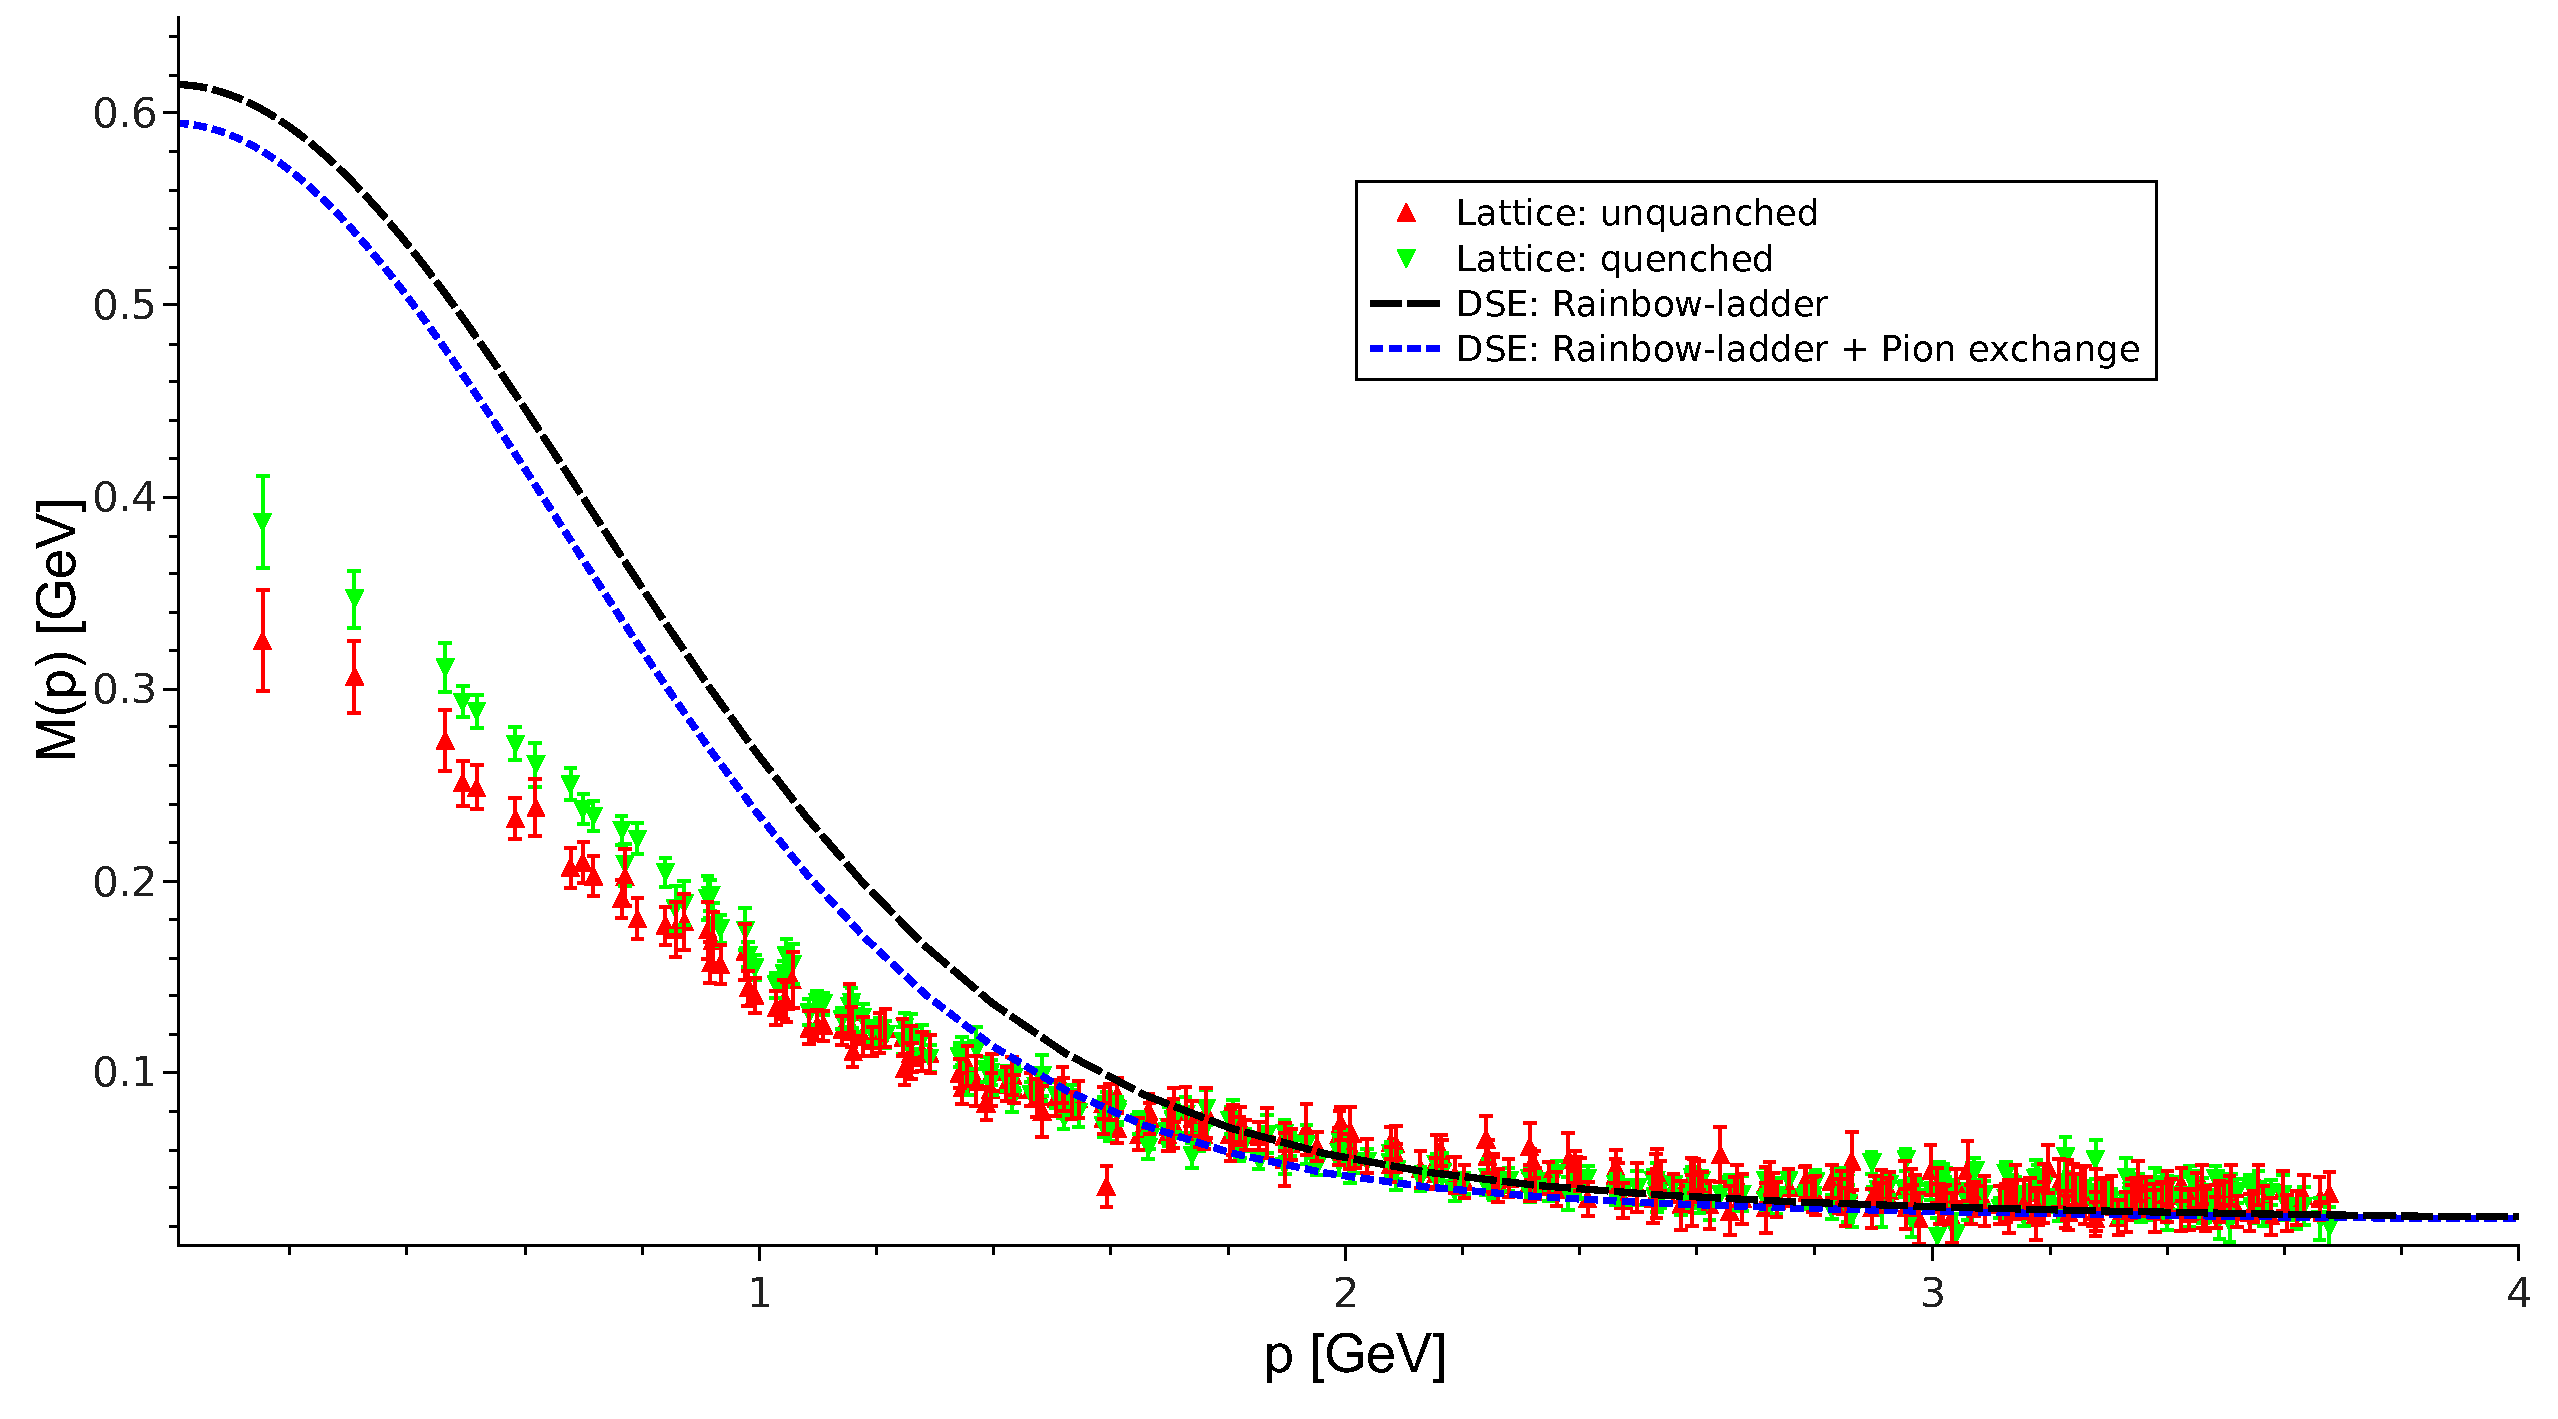
\includegraphics[width=0.95\textwidth]{figures/DSE_vs_Lattice}
 \end{center}
 \caption{\footnotesize The impact of pion cloud effect on $M(p^2)$ quark mass function.  }\label{fig:DSE_vs_Lattice} 
\end{figure}
	Also we compared our result to the lattice data on quenched and unquenched quark mass function in order to check the impact of unquenching effects, i.e. pion clouds with the lattice QCD. From the Fig. \ref{fig:DSE_vs_Lattice} we see that although the absolute value of $M(p^2)$ in infrared does not coincide with our calculations, the relative changes induced by unquenching pion cloud effect are of the similar size. It was shown in \cite{Fischer:2008sp}, that the usage of Ball-Chu vertex can provide a better agreement with lattice data. However, the inclusion of the pion exchange does not produce any qualitative difference in a behaviour of dressing functions, e.g. the most significant change happens in $M(p^2)$ quark mass function, where pion clouds lead to shrinking dynamical mass generation in infrared region by 10 percent. \\
		
Also it is important to consider the order parameter of dynamical chiral symmetry breaking - the quark condensate \cite{Miransky:271593}. Recall that in perturbative theory in chiral limit $m_q\rightarrow 0$ the dressing function $B(p^2)=0$ and therefore the mass function $M(p^2)=B(p^2)/A(p^2)=0$ as well. However as we see from Fig. \ref{fig:quark_M_func} the $M(P^2)$ is not zero in chiral limit. Thus, the quark condensate:
\beqa
	\langle \bar q q \rangle &=& - \lim_{\Lambda \rightarrow \inf} Z_4(\mu,\Lambda) \int^\Lambda \frac{d^4 k}{(2\pi)^4} \Tr \Bigl[ S_{m_bare = 0}(k) \Bigl] \\
	&=& - \lim_{\Lambda \rightarrow \inf} Z_4(\mu,\Lambda) \int^\Lambda \frac{d^4 k}{(2\pi)^4} \Tr \Bigl[ \frac{B(p^2)}{p^2A^2(p^2) + B^2(p^2)} \Bigl]\;,
\eeqa
is nonzero by virtue of a nonzero $B(p^2)$. Here $Z_4$ is quark mass renormalization constant, given by:
\beqa
	Z_4 = 2 - \frac{B(\mu^2,\Lambda^2)}{m_R(\mu^2)}
\eeqa
The resulting value for the quark condensate in rainbow-ladder and in pion cloud truncation are given in Table. \ref{tab:quark_cond}.
\begin{table}[!h]
\centering
\renewcommand{\arraystretch}{1.3}
\begin{tabular*}{0.70\textwidth}{@{\extracolsep{\stretch{1}}}c|c|c|c@{}}
\hline
\hline
 & RL1 & RL2 & RL2 + pion cloud \\
\hline
$\langle \bar q q\rangle \; [MeV]$  & 281 & 300 & 280 \\
\hline
\hline
\end{tabular*}
\caption{The values of the quark condencate for a rainbow-ladder and pion cloud truncation in comparisson.  \label{tab:quark_cond}}
\end{table}
 However, as we will see from Chapter\;4 the nonzero $B(p^2)$ in chiral case still generates the massless pion, thus ensuring the pions to be the Goldstone bosons. \\
%	
\subsection*{Continuation into time-like region}
The solutions of quark \DS equations we obtained so far are already a very valuable source of information about dynamical chiral symmetry breaking. However, as we stated earlier, the parameters of effective coupling should be fitted in a such way that the pion mass and weak decay constant are reproduced by \BS equation (BSE) of pion bound state. And this equations itself requires as input the solutions of the quark \DS equations (DSE). Due to certain kinematic scheme of BSE, which will be clarified in Chapter 5, the input from quark DSE must be provided partially in time-like region $p^2 < 0$. Namely on the contour in complex plane, which parametric form is defined by mass of bound state to be calculated:
\beqa
	p^2 = t^2 + itM_{state} - \frac{M_{state}^2}{4} 
	\label{dse:contour}
\eeqa
For the parameter $t \in [-\infty, \infty]$ defining the contour in complex plane, in our computations we use Legendre integration nodes. This specific form of the contour will be derived later, when the details of kinematic of the bound state BSE will be considered. \\
	
Brute-force way to the continuation is to invoke the Eq. (\ref{dse:DSE_RL}) on complex $p$-momentum, using space-like the solution $S(k)$ as input in equations. In this case the relative momenta $q=p-k$ will become complex as well and effective coupling model will be invoked in time-like region. There are several issues associated with the analytic continuation in this kinematic scheme: on one hand, the $q$-momentum is no longer real and therefore usage of Maris-Tandy(MT) model Eq. (\ref{dse:MT_model}) may produce numerical glitches; on another hand, in the pion propagator, given in form: $D_\pi(q^2)=\frac{1}{q^2+M^2_\pi}$, complex $q$-momenta will probe the pion pole, therefore diverging any integration. Thus this kinematic scheme can only be applied for Rainbow-ladder calculation. \\
	The resulting continuation in $\sigma_v = \frac{A}{A^2 p^2 + B^2}$ dressing function for quark propagator are given is Fig. \ref{fig:sigma_poles}. 
\begin{figure}
\tiny
 \begin{center}
  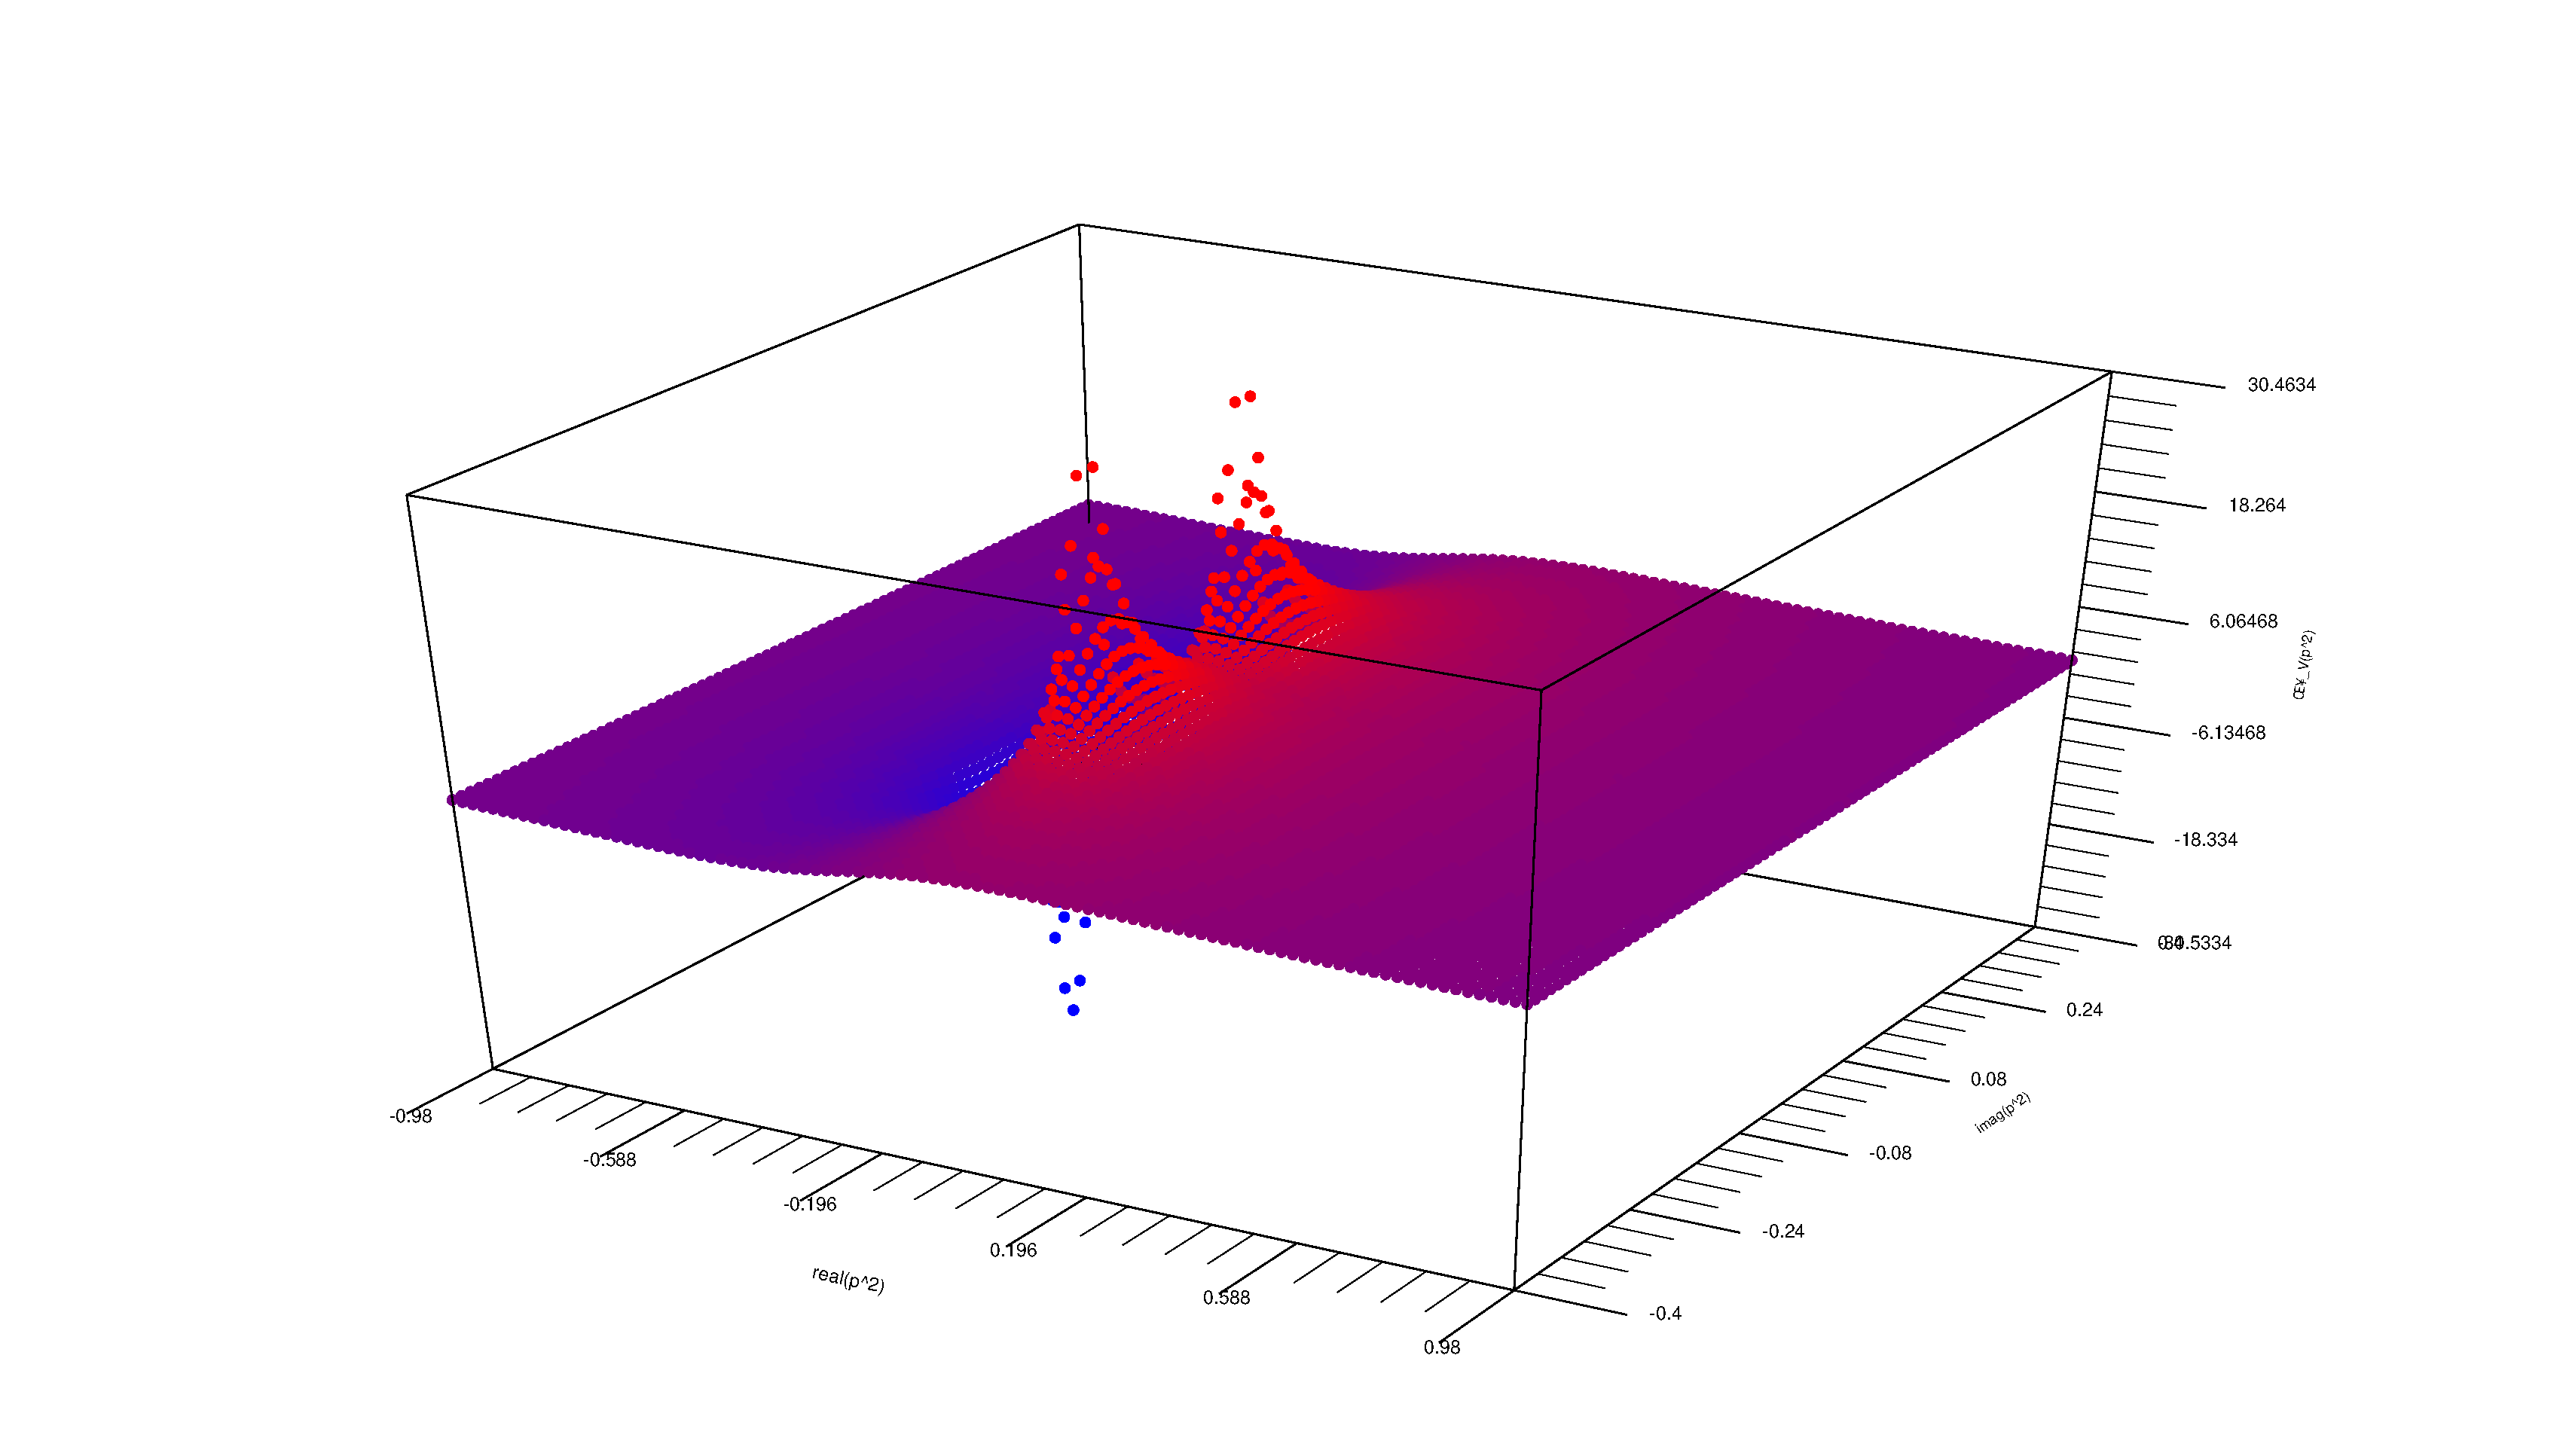
\includegraphics[width=1.1\textwidth]{figures/sigma_poles}
 \end{center}
 \caption{\footnotesize Analytic continuation of quark dressing $\sigma_V$. }\label{fig:sigma_poles} 
\end{figure}

Recall, the inverse quark propagator is given in the form:
\beqa
	S(p) =i \sigma_v(p^2) \pslash + \sigma_s(p^2)\;,
\eeqa
whether the inverse one:
\beqa
	S^{-1}(p)=-i A(p^2)\pslash + B(p^2)
\eeqa
	As we can see from Fig. and Fig. the quark propagator has two poles, that come from the common denominator in $\sigma_v$ and $\sigma_s$ functions:
\beqa
	\frac{1}{A^2 p^2 + B^2}
\eeqa
Note however, these poles are not corresponding to asymptotic state, since they are not lying on real $P^2$ axis. Also it was shown in \cite{Fischer:2008sp} that the inclusion of the pion cloud effect does not change the non-analytic structure of the quark, as it was required from Gribov's supercriticality picture of quark confinement.
\begin{figure}[H]
\tiny
 \begin{center}
  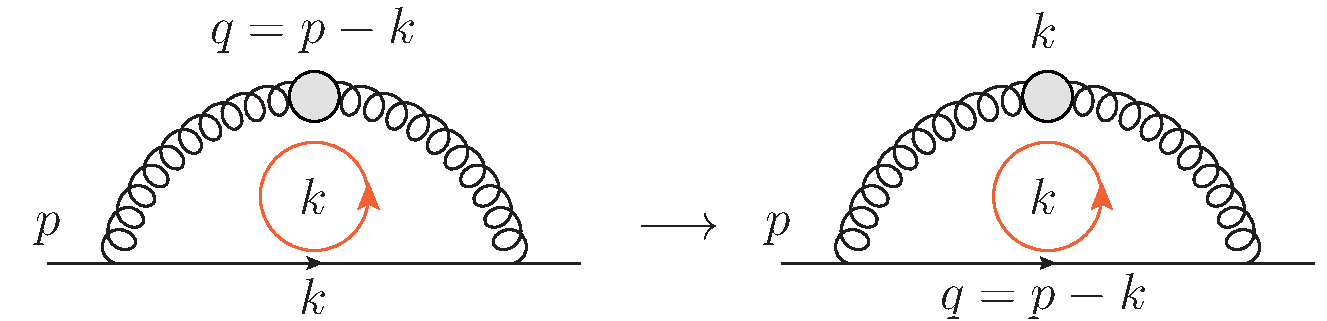
\includegraphics[width=0.95\textwidth]{figures/shift_momenta}
 \end{center}
 \caption{\footnotesize Shifting momenta routing. }\label{fig:shift_momenta} 
\end{figure}
	In order to be able to perform similar continuation for the DSE with pion cloud effect included we need to change momenta routing in a such way, that integration real $k$-momentum would flow through gluon and pion propagators and complex $q=p-k$ would go though quark propagator. This is diagrammatically given in Fig. \ref{fig:shift_momenta}. This allows us to solve two problems in the same time: firstly, use Maris-Tandy model on real axis as it is meant to be used; secondly, do not hit a pole in pion propagator $D_\pi(k^2)=\frac{1}{k^2+M^2_\pi}$. However it requires more sophisticated numerical approach in order to solve quark DSE - so-called "Grid-to-Contour" iteration, which is described in Appendix \ref{app:numerics}. \\ 
	
	At this point we considered a key piece in whole DSE/BSE calculation framework: the quark \DS equations. We studied its various truncations and physical meaning behind them. We obtained the solutions associated with quark DSE in rainbow-ladder and pion cloud truncations, observed the dynamical chiral symmetry breaking and continued these solutions into time-like region for the further use in meson \BS equations. 
\chapter{QCD Bound States}
\label{chap:BSE}
\section{Bethe-Salpeter equation}
\label{bse}
Bound states in QCD are composite color-scalar objects made of color-carrying particles. Starting from common two-body state $q \bar q$ like meson and three-body state $qqq$ like baryon, and ending with exotic not-yet-detected-but-possibly-existing states like tetraquarks $qq \bar q \bar q$, glueballs $GG$ and hybrids $qqG$. Due to usual form of propagator of massive particle $\frac{1}{p^2 + M^2}$ a bound state produce a pole in the scattering amplitude in the corresponding channel. For a composite bound state, the pole can not be generated by any finite sum of Feynman diagrams \cite{9780471353867}, but only by infinite series. However it is not possible in general, so instead we may consider to strive for an infinite sum of diagrams of a particular class, which are we assume to be dominant and crucial for a given process (i.e. all ladder diagrams). This can be archived by finding an appropriate integral equation, the solutions of which can be interpreted as the result of such particular summation. \\

	In order to derive aforementioned integral equation let us consider the \DSE for quark-antiquark scattering amplitude:
\beqa
	M(p,q;P) = K(p,q;P) + \int \frac{d^4k}{(2\pi)^4} K(p,k;P) G(k,P) M(k,q;P)\;,
	\label{bse:M_DSE}
\eeqa
where $M(p,q;P)$ is the scattering amplitude, $G(k,P)$ is two-quark full propagator, $K(p,q;P)$ is the two-body irreducible scattering kernel. This equations is illustrated diagrammatically on Fig. \ref{fig:M_DSE}.
\begin{figure}[H]
\tiny
 \begin{center}
  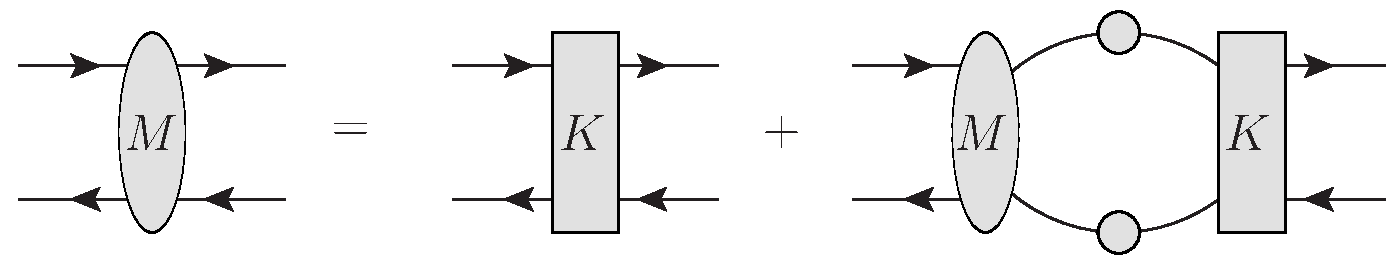
\includegraphics[width=0.95\textwidth]{figures/M_DSE}
 \end{center}
 \caption{\footnotesize \DSE  of quark-antiquark scattering amplitude. The dots on quark lines denote dressed (full) quark propagators }\label{fig:M_DSE} 
\end{figure}
If the kernel is "small", so that the perturbation series converge, the solution of Eq. (\ref{bse:M_DSE}) can be obtained by iteration. The following Born series schematically take the form:
\beqa
	M = K + \int KGK + \int \int KGKGK + \;...\; + \left(  \int KG \right)^n K +\; ...
	\label{bse:M_sum}
\eeqa

After replacing the integrals in Eq. (\ref{bse:M_sum}) by sums over discrete points in momentum, so that $K$ and $M$ are matrices and $G$ a diagonal matrix, when the Eq. (\ref{bse:M_sum}) can be formaly considered as a geometric sum, giving:
\beqa
	M &=& K + KGK + KGKGK + \;...\; + (KG)^n K +\; ... \\
	 &=& (1-KG)^{-1}K
	 \label{bse:M_sum2}
\eeqa
This expressions is similar to the simple complex function:
\beqa
	f(z)=\frac{z}{1-z}\;,
\eeqa
which is the unique analytic continuation of the series:
\beqa
	f(z)=\sum_n z^n\;,
\eeqa
from the unit circle $|z|<1$ to the region outside, $|z|\geq 1$, with the pole at $z=1$. In case $z$ being a matrix, one can generalize that $z$ has the eigenvalue $\lambda$ equal to one, so that the corresponding condition can be written as:
\beqa
	\mathbf{e} = z \mathbf{e}\;,
\eeqa
where $\mathbf{e}$ is the eigenvector. Therefore in case of Eq. (\ref{bse:M_sum2}) the condition for a pole in the scattering amplitude $M$ is following:
\beqa
	\Gamma(p;P) = \int_k K(p,k;P)G(k,P)\Gamma(k;P)\;,
\eeqa
here $\int_k$ denotes 4-momenta integration with appropriate weight. Apparently, this is the integral equation for a bound state, and $\Gamma$ refers to the bound state wave function. As a final step we need to write explicitly the two-quark full propagator $G=S\Gamma S$, so the equation writes as:
\beqa
	\Gamma^{(\mu...)}_{tu}(p;P) = \lambda(P^2) \int \frac{d^4 k}{(2\pi)^4} K_{tu;rs}(p,k;P)\left[ S(k_+)\Gamma^{(\mu...)}(k;P)S(k_-)\right]_{sr}\;,
	\label{bse:BSE_gen}
\eeqa
where the $\lambda(P^2)$ is eigenvalue. This is the \textit{homogeneous (on-shell)} Bethe-Salpeter equation (BSE) \cite{PhysRev.84.1232, PhysRev.84.350} and the function $\Gamma$ is vertex function, whose dressing functions are so-called the Bethe-Salpeter Amplitudes (BSA). The $tu;rs$ denote a relevant Dirac indexes and $(\mu...)$ reflect the Lorenz structure of the wave function. We will address an explicit representations of basis tensors later. The momenta $k_+,k_-$ obey the momenta conservation law $k_+ - k_- = P$, where $P^2=-M^2_{meson}$ is the meson mass shell. This allow us to represent $k_+,k_-$ as:
\beqa
	k_+ &=& k + \zeta P\;, \\
	k_- &=& k - (1-\zeta) P\;,
\eeqa
where $\zeta \in (0,1)$ is \textit{partitioning parameter} specifying the fraction of $P$ carried by quarks. Note that the out-coming results are independent of $\zeta$, however varying this parameter may increase the numerical complexity. Therefore for quark symmetric bound states like: $\bar n n, \bar s s, \bar c c$, etc. we employ the equal partitioning $\zeta=\frac{1}{2}$. %In case of quark asymmetric meson like: $\bar n s, \bar c s$, etc. the optimal partitioning is provided in Appendix [CITE].
 The Eq. (\ref{bse:BSE_gen}) is diagrammatically given on Fig. \ref{fig:BSE_gen}.
\begin{figure}[H]
\tiny
 \begin{center}
  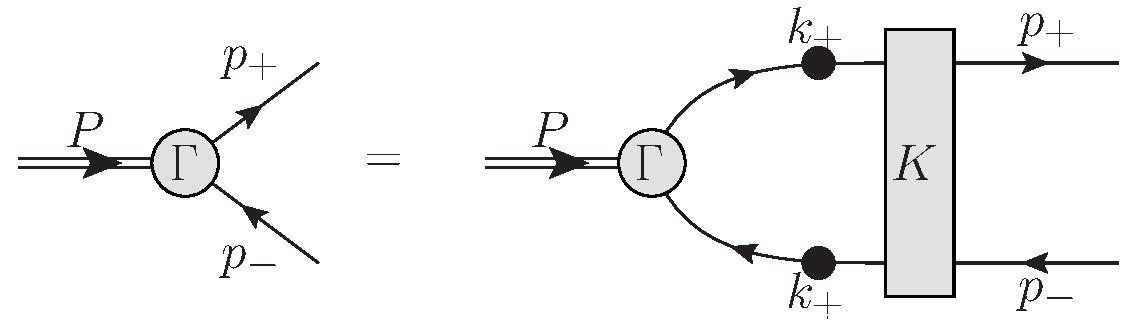
\includegraphics[width=0.95\textwidth]{figures/BSE_gen}
 \end{center}
 \caption{\footnotesize The meson \BS equations. }\label{fig:BSE_gen} 
\end{figure}
This equations is a sufficient and necessary condition for a pole to appear in $M$ 4-point Green's function at $P^2=-M^2_{meson}$. Numerically this means we need to solve inverse problem, so that we need to search for the $P^2$ such that $\lambda(P^2)=1$. \\ 

The Eq. (\ref{bse:BSE_gen}) can be transformed to \textit{inhomogeneous (off-shell)} by adding a bare term to \BSE:
\beqa
	\Gamma^{(\mu...)}(p;P) = \Gamma^{(\mu...)}_{0}(p;P) + \int_k K(p,k;P)\left[ S(k_+)\Gamma^{(\mu...)}(k;P)S(k_-)\right]\;,
	\label{bse:BSE_inhom}
\eeqa
here the $\Gamma^{(\mu...)}_{0}$ is a bare tern, which obviously must have the same Dirac and Lorenz structure as the full one $\Gamma^{(\mu...)}$, but the BSA equal one. The off-shell meson BSE is illustrated on Fig. \ref{fig:BSE_gen_offshell}.
\begin{figure}[H]
\tiny
 \begin{center}
  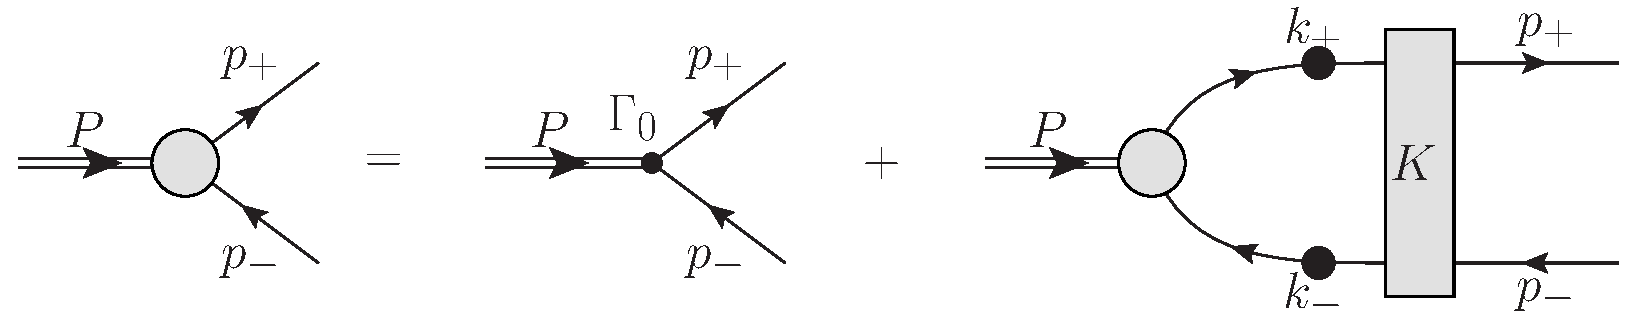
\includegraphics[width=0.95\textwidth]{figures/BSE_gen_offshell}
 \end{center}
 \caption{\footnotesize The inhomogeneous (off-shell) meson \BS equations. }\label{fig:BSE_gen_offshell} 
\end{figure}
Note that the inhomogeneous BSE given by Eq.(\ref{bse:BSE_inhom}) is no longer an eigenvalue problem, therefore has to be solved iteratively. The detailed instructions are given in Appendix \ref{app:numerics}.

\section{Total angular momentum tensor}
\label{bse:angular_tensor}
With the truncation set we are close to perform the inevitable calculations, however, the last piece from a recipe is missing. If we make a look on meson \BSE again:
\beqa
	\Gamma^{(\mu...)}_{tu}(p;P) = \lambda(P^2) \int \frac{d^4 k}{(2\pi)^4} K_{tu;rs}(p,k;P)\left[ S(k_+)\Gamma^{(\mu...)}(k;P)S(k_-)\right]_{sr}\;,
\eeqa
we see that the Dirac and Lorenz structure of $\Gamma^{(\mu...)}_{tu}(p;P)$ yet still unspecified and therefore the quantum numbers $J^{PC}$ of the meson under considerations are not yet determined. In order to do so, we choose the appropriate basis for $\Gamma^{(\mu...)}_{tu}(p;P)$, such the quantum numbers $J^{PC}$ of the meson would be clear. \\

It is well known that composite states of particles in the $\left(j,0\right)\oplus\left(0,j\right)$-representation can be constructed 
by forming direct products of the particle's representation~\cite{Joos:1962qq,Weinberg:1964cn}. For fermions, $j=1/2$, this reduces
to the Dirac spinor formalism and thus is given by the usual Dirac matrices. \\

For a meson in the rest frame with center-of-mass momentum $P_\mu$ and
relative quark momentum $p_\mu$, grouped by their transformation under parity we have
%
\begin{align}\label{eqn:scalarinvariants1}
D^{(\ONE)}&=
\left(\begin{array}{ccccc}
\;\ONE\; &
\phantom{\gamma_5}P_\mu \gamma^\mu\;&
\phantom{\gamma_5}p_\mu \gamma^\mu\;&
\phantom{\gamma_5}p_\mu P_\nu \frac{1}{2}\left[\gamma^\mu,\gamma^\nu\right]
\end{array}\right)\;, \\
%
D^{(5)}&=
\left(\begin{array}{ccccc}
\gamma_5\;&
\gamma_5 P_\mu \gamma^\mu\;&
\gamma_5 p_\mu \gamma^\mu\;&
\gamma_5 p_\mu P_\nu \frac{1}{2}\left[\gamma^\mu,\gamma^\nu\right]
\end{array}\right)\;,
\end{align}
%
for scalar, $D^{(\ONE)}$, and pseudoscalar, $D^{(5)}$, invariants respectively. Thus, for a 
bound-state of two fermions with definite parity, the basic number of scalar invariants equals
four. Furthermore, it is convenient to replace the relative momentum $p_\mu$ by
%
\begin{align}\label{eqn:transverseQ}
Q_\mu = \tau^{(P)}_{\mu\nu}\;p^\nu\;,
\end{align}
%
where $ \tau^{(P)}_{\mu\nu}=\delta_{\mu\nu}-P_\mu P_\nu/P^2$ is a transverse projector.
%
Then, appropriate scalar and pseudoscalar invariants are
%
\begin{align}\label{eqn:scalarinvariants2}
\bar{D}^{(\ONE)}&=
\left(\begin{array}{ccccc}
\;\ONE\; &
\phantom{\gamma_5}\slashed{P}\;&
\phantom{\gamma_5}\slashed{Q}\;&
\phantom{\gamma_5}\slashed{Q}\slashed{P}
\end{array}\right)\;,\;\;\;\;
%
\bar{D}^{(5)}=\gamma_5\bar{D}^{(\ONE)}\;,
\end{align}
%
which simplifies the operation of charge conjugation due to the fact that $Q\cdot P=0$.\\

Then, a bound state with zero total angular momentum and definite parity is decomposed in terms of 
four components
%
\begin{align}
\Gamma^{(Parity)}(p,t) &= \sum_{i=1}^{4} \left[A_i  \bar{D}_{i}^{(Parity)}\right]\;,
\end{align}
where $A_i$ denotes \BS amplitude - the scalar dressing function. 

For non-zero total angular momentum $J$, the $A_i$ scalar invariants
must be coupled with an angular momentum tensor. This rank $J$ tensor, $T_{a_1,\ldots a_J}$, has 
$2J+1$ independent components in three spatial dimensions, corresponding to the possible spin 
polarisations~\cite{Zemach:1968zz}. This tensor must be 
symmetric in all indices and traceless with respect to contraction of any pair of indices.
This generalizes to $3+1$ dimensions by imposing transversality of each 
index with respect to the total momentum.

Thus, to obtain a tensor corresponding to total angular momentum $J$, we construct the 
symmetric $J$-fold tensor product of a transversal projector transforming like a vector, and 
subtract traces with respect to every pair of indices. 

Then, in general a meson of spin $J>0$ and parity $P$ has eight components and is written
%
\begin{align}
\Gamma^{(Parity)}_{\mu_1\ldots\mu_J}(p,P) &= \sum_{i=1}^{4} \left[A_i Q_{\mu_1\ldots\mu_J} \bar{D}_{i}^{(Parity)}+A_{i+4} T_{\mu_1\ldots\mu_J} \bar{D}_{i}^{(Parity)}\right]\;,
\end{align}
%
where the $Q_{\mu_1\ldots\mu_J}$, $T_{\mu_1\ldots\mu_J}$ are defined below and $A_i = A_i(p,P)$. The explicit expressions for $J = 1,2,3$ can be found in Appendix \ref{app:basis}. Therefore by choosing appropriate basis can define the $J^{PC}$ quantum numbers of the meson under consideration. 

\subsection*{Axial-vector Ward Takahashi Identity}
\vspace{-0.5cm}
In previous chapter we saw how the phenomena of dynamical symmetry breaking appear in calculation, by observing a nonzero order parameter, namely, the quark condensate $\langle \bar q q \rangle$. This fact together with appearance of massless pion in the meson spectrum is a clear indication of dynamical chiral symmetry breaking in QCD, where pions are 	identified with the Goldstone bosons of the broken symmetry. The satisfaction of axial-vector Ward Takahashi Identity (axWTI) is crucial for a proper description of this phenomena within the \DS - \BSE approach \cite{Maris:1997hd}. Moreover, as we will see, the satisfaction of axial-vector Ward Takahashi Identity provides the pion vertex ansatz, shown in Eq.(\ref{dse:pion_vertex}). \\ 

The axial-vector Ward Takahashi Identity in chiral limit takes the following form:
\beqa
	-iP_\mu \Gamma^j_{5\mu}(k;P) = S^{-1}(k_+)\gamma_5\frac{\tau^j}{2} + S^{-1}(k_-)\gamma_5\frac{\tau^j}{2}\;,
	\label{bse:axWTI}
\eeqa
where the axial-vector vertex is:
\beqa
	\Gamma^j_{5\mu}(k;P) &=& \frac{\tau^j}{2}\gamma_5[\gamma_\mu F(k;P) + \gamma \cdot k k_\mu G(k;P) - \sigma_{\mu\nu}k_\nu H(k;P)] \\
	&+& f_\pi\frac{P_\mu}{P^2} \Gamma^j_\pi(k;P)\;,
	\label{bse:ax_vertex}
\eeqa
$f_\pi$ is pion weak decay constant and $\Gamma_\pi$ is general pion wave function, with the decomposition given in Eq.(\ref{dse:pion_vertex_gen}). Substituting Eq.(\ref{bse:ax_vertex}) and Eq.(\ref{dse:pion_vertex_gen}) into Eq.(\ref{bse:axWTI}) and taking limit $m^2_\pi \rightarrow 0$ one obtains the chiral limit relations between pion dressing functions and quark dressing functions \cite{Maris:1997tm}:
\beqa
	f_\pi E_\pi(k;0) = B(p^2) \\
	F(k;0) + 2f_\pi F_\pi(k;0) = A(p^2) \\
	G(k;0) + 2f_\pi G_\pi(k;0) = 2A(p^2) \\	
	H(k;0) + 2f_\pi H_\pi(k:0) = 0 \;,
	\label{bse:axWTI_relation}
\eeqa
where $E_\pi$, $F_\pi$, $G_\pi$ and $H_\pi$ are scalar dressing functions of the pion \BS amplitude. And the pion electroweak decay constant can be calculated via:
\beqa	
	f_\pi = \frac{Z_2N_C}{m^2_\pi} \int \frac{d^4 k}{(2\pi)^2} P_\mu Tr \Bigl[ \Gamma_\pi(k;P) S(k_-) \gamma_\mu \gamma_5 S(k_+) \Bigl]\;,
\eeqa
here $N_C$ is the color factor. Note however, the full pion vertex $\Gamma_\pi$ has to be properly normalized.
\section{Normalization of the BSA}
The meson bound state equation Eq.(\ref{bse:BSE_gen}) and eigenvector $\Gamma$ is defined up to arbitrary multiplicative factor, to fix which we need to impose the normalization condition on $\Gamma$. The canonical normalization \cite{1969PThPS..43....1N} has the following form:
\beqa
\notag	1 &=& 2\frac{\partial}{\partial P^2} Tr \int \frac{d^4 k}{(2\pi)^4} \Bigl[  3(\bar \Gamma(k, -Q) S(k + P/2) \Gamma(k, Q) S(k - P/2)) \;\;\;\;\;\;\;\;\;\; \\
	 &+& \int \frac{d^4 k^{\prime}}{(2\pi)^4} ( \bar \chi (k^{\prime}, -Q) K(k^{\prime} ,k;P) \chi(k,Q) ) \Bigl] \;,
	 \label{bse:Norm1}
\eeqa
where $Q^2 = - M^2_{meson}$ is fixed on mass shell and the Bethe-Salpeter wave-function is defines as:
\beqa
	\chi(k;P) = S(k + P/2)\Gamma(k;P)S(k - P/2)
\eeqa
The charge conjugated vertex function $\bar \Gamma$ is given by:
\beqa
	\bar \Gamma(k;P) = C\Gamma^{T}(-k;P)C^{-1}\;,
\eeqa
here $C=-\gamma_2\gamma_4$ is a charge conjugation matrix and index $T$ denotes the transpositioning. \\

Although the Eq.(\ref{bse:Norm1}) is a valid way to normalize $\Gamma$, it requires significant numerical efforts, since for it involves double momenta integration. Therefore it is useful to consider alternative way to normalize BSA, given by \cite{PhysRev.138.B1182,PhysRev.139.AB1,Fischer:2009jm}:
\beqa
	\Bigl( \frac{1}{\lambda}\frac{\partial \lambda}{\partial P^2} \Bigl)^{-1} = \int \frac{d^4 k}{(2\pi)^4} Tr \Bigl[ \bar \Gamma(k, -P) S(k + P/2) \Gamma(k, P) S(k - P/2)) \Bigl]\;,
	\label{bse:Norm2}
\eeqa
where the eigenvalue $\lambda=1$ at $P^2=-M^2_{meson}$. This normalization equations is beneficial, since it requires only one-loop integration and independent of the employed truncation.

\section{Scattering kernel K}
So far we discussed a general meson \BSE without specifying the truncation of BSE, which uniquely defined by truncation imposed on quark \DSE before. The reason for such connection is that the solutions of pion BSE must fulfil the axial-vector Ward Takahashi Identity in order to provide the dynamical chiral symmetry breaking and fulfil Gell-Mann-Oakes-Renner relation (GMOR), given by Eq.(\ref{qcd_low:GMOR}) in case of the explicit chiral symmetry breaking. \\
\begin{figure}[H]
\tiny
 \begin{center}
  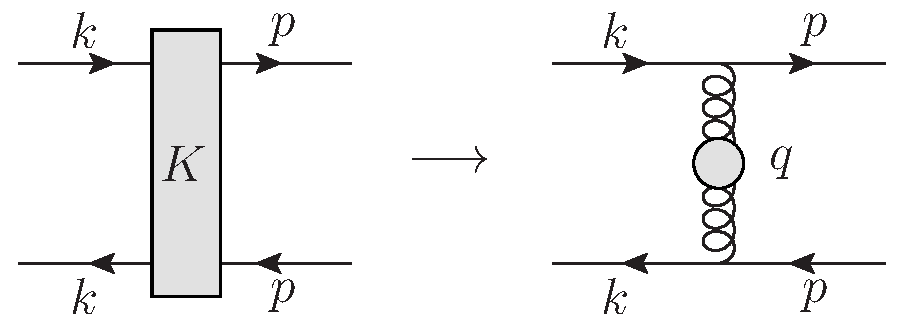
\includegraphics[width=0.75\textwidth]{figures/RL_kernel}
 \end{center}
 \caption{\footnotesize Rainbow-ladder effective one gluon exchange kernel. The filled dot represents the effective dressing via $\alpha_{\mathrm{eff}}(q^2)$. }\label{fig:RL_kernel} 
\end{figure}
In case of effective one gluon exchange also known as rainbow-ladder truncation as it was discussed in the previous chapter, the two-body scattering kernel $K(p,k;P)$ takes the following form:
\beqa
	K_{tu;rs}(p,k;P) = Z_2^2 \Bigl( \delta^{\mu\nu} - \frac{q^\mu q^\nu}{q^2} \Bigl)  \frac{\alpha_{\mathrm{eff}}(q^2)}{q^2}
	\Bigl[ \frac{\lambda^a}{2}\gamma^\mu \Bigl]_{ts} 
	\Bigl[ \frac{\lambda^a}{2}\gamma^\nu \Bigl]_{ru} \;,
	\label{bse:RL_kernel}
\eeqa
where $\lambda^a$ are Gell-Mann matrices, the $q=p-k$ is relative momentum, the indexes $\{tu;rs\}$ denote explicitly Dirac indexes, $Z_2$ is renormalization constant from quark DSE and $\alpha_{\mathrm{eff}}(q^2)$ is the same model for effective coupling as in Eq.(\ref{dse:MT_model}), used with the same parameters as for quark DSE calculation. This Eq. (\ref{bse:RL_kernel}) kernel is illustrated diagrammatically on Fig. \ref{fig:RL_kernel}. \\

In case of the unquenching pion cloud effect we need to introduce an additional contribution to the two body kernel, so can be represented as a sum:
\beqa
	K(p,k;P) = K^{gluon}(p,k;P) + K^{pion}(p,k;P)\;,
	\label{bse:PS_kernel}
\eeqa
where $K_{gluon}(p,k;P)$ is given by Eq.(\ref{bse:RL_kernel}) and $K_{pion}(p,k;P)$ is effective one pion exchange scattering kernel. The explicit view of $K_{pion}(p,k;P)$ takes the following form \cite{Fischer:2008wy,Fischer:2008sp}:
\beqa
	K^{pion}_{tu;rs}(p,k;P) &=& \frac{1}{4}[\Gamma^j_\pi]_{ru}  \left( \frac{p+k-P}{2};p-k \right)[Z_2 \tau^j \gamma_5]_{ts} D_\pi(q^2)\\
\notag	&+& \frac{1}{4}[\Gamma^j_\pi]_{ru}  \left( \frac{p+k-P}{2};k-p \right)[Z_2 \tau^j \gamma_5]_{ts} D_\pi(q^2) \\
\notag 	&+& \frac{1}{4}[\Gamma^j_\pi]_{ru}  \left( \frac{p+k+P}{2};p-k \right)[Z_2 \tau^j \gamma_5]_{ts} D_\pi(q^2) \\
\notag 	&+& \frac{1}{4}[\Gamma^j_\pi]_{ru}  \left( \frac{p+k+P}{2};k-p \right)[Z_2 \tau^j \gamma_5]_{ts} D_\pi(q^2) \;,
	\label{bse:pion_kernel}
\eeqa
here $\tau^j$ is a $SU(2)$ isospin Pauli matrices and the pion propagator $D_\pi$ in the same form as it was used in quark DSE:
\beqa
	D_\pi(q^2)=\frac{1}{q^2 + m^2_\pi}
\eeqa
The extended kernel in Eq.(\ref{bse:PS_kernel}) is represented illustratively on Fig. \ref{fig:PS_kernel}..
\begin{figure}[!]
\tiny
 \begin{center}
  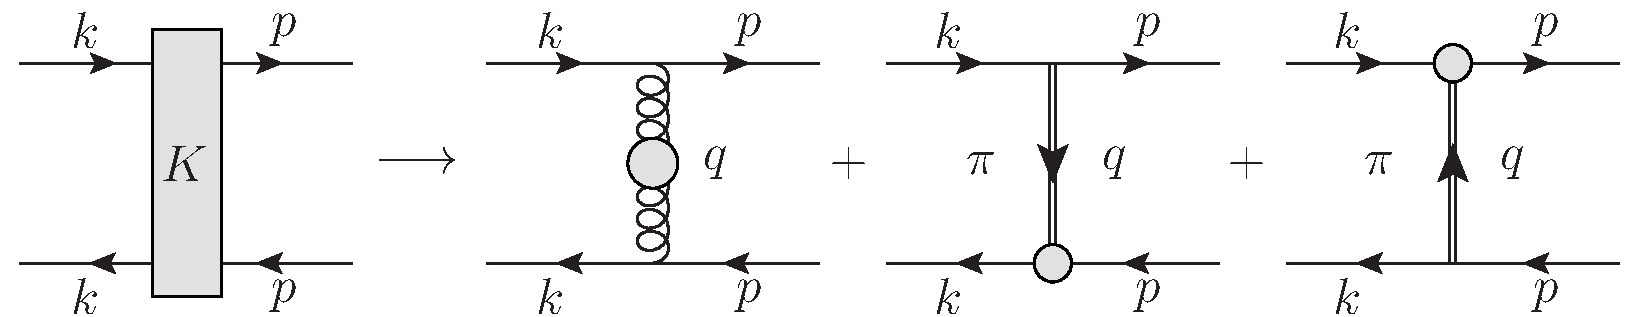
\includegraphics[width=0.99\textwidth]{figures/PS_kernel}
 \end{center}
 \caption{\footnotesize Rainbow-ladder effective one gluon and pion exchange kernel. The double line represents the pion propagator $D_\pi$ and filled dots on pion exchange diagrams denote pion vertex $\Gamma_\pi$. }
 \label{fig:PS_kernel} 
\end{figure}
However, alike in case of quark \DSE, as a pion vertex $\Gamma_\pi$ we employ the same approximation as we did in quark DSE in previous chapter:
\beqa
	\Gamma_\pi(p;P) = \gamma_5 E(p;P) = \gamma_5\frac{B(p^2)}{f_\pi}
	\label{bse:pion_vertex}
\eeqa
This approximation has negligible difference, since the first pion amplitude $E(p;P)$ is dominant, but provides the significant numerical simplification. Apparently, the Eq.(\ref{bse:pion_vertex}) naturally follows from Eq.(\ref{bse:axWTI_relation}). Recall, for the high pion mass calculations we used explicitly calculated first pion amplitude $E(p;P)$ in rainbow-ladder approach. \\

Finally, note that the interaction kernel Eq.~(\ref{bse:pion_kernel}) is not the 
full story in terms of diagrams. If the kernel were derived by the usual 
'cutting of diagrams' procedure as e.g. in a 2PI approach \cite{Munczek:1994zz}, 
a diagram would appear containing two internal pions. Such a diagram 
contains the important physics of opening up two-pion decay channels for certain
kinematics, relevant for example in the vector-meson sector. At present the resulting 
two-loop diagrams in the quark-antiquark interaction have not been addressed in the
DSE/BSE approach due to the numerical complexity involved. While a more complete approach finally has 
to deal with the two-loop diagram, in this exploratory calculation we will 
resort to the ladder contribution only.   \\

\section{Fadeev equation}
The 3-body bound state equation can be derived in a similar way as a meson BSE in Section \ref{bse}. One has to consider the \DSE for the three-quark scattering amplitude $M_(qqq)$ and applying the same idea as of dominant bound state pole contribution to $M_(qqq)$, one can derive the 3-body bound state equation, so-called Faddeev equation, that defines the mass and internal structure of baryons. Within Faddeev equation framework were performed covariant three-body calculations of nucleon, delta and omega masses \cite{Eichmann:2009qa,Eichmann:2009en,SanchisAlepuz:2011jn} as well as their electromagnetic elastic and transition form factors \cite{Eichmann:2011vu,Eichmann:2011aa,Sanchis-Alepuz:2013iia}.
  The Faddeev equation in its explicit form reads as:
\begin{equation}\label{fad:3bBSEcompact}
\Psi = -i\widetilde{K}^{(3)}~G_0^{(3)}~\Psi + \sum_{a=1}^3 -i\widetilde{K}_{(a)}^{(2)}~G_0^{(3)}~\Psi\,,
\end{equation}
where $\widetilde{K}^{(3)}$ and $\widetilde{K}^{(2)}$ are the three- and two-body interaction kernels, respectively, and $G_0$ represents the product of three fully-dressed quark propagators $S$. We used here a compact notation where indices have been omitted and we assume that discrete and continuous variables are summed or integrated over, respectively. 
The spin-momentum part of the full amplitude $\Psi$ depends on 
the total and two relative momenta of the three valence quarks inside 
the baryon. As discussed in more detail in Section \ref{subsec:internal_composition}, 
this amplitude contains all possible spin and orbital angular momentum contributions.
\begin{figure*}[h]
 \begin{center}
  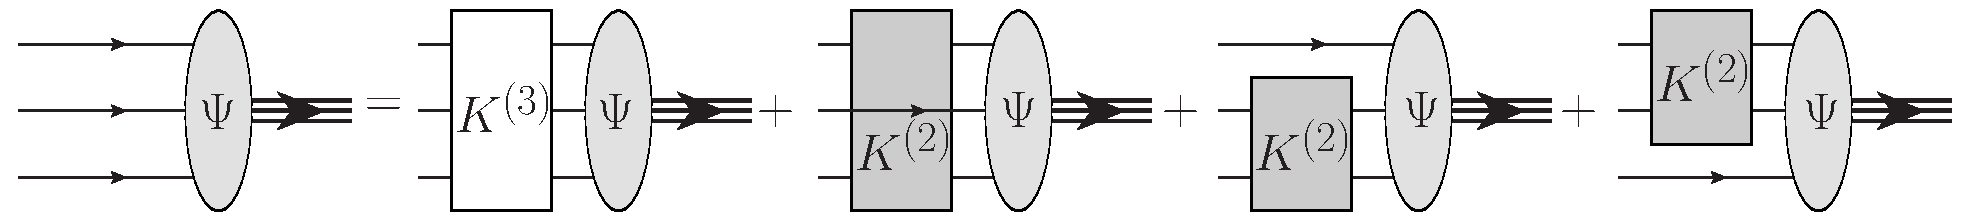
\includegraphics[width=0.99\textwidth]{figures/Faddeev}
 \end{center}
 \caption{Diagrammatic representation of the three-body Bethe-Salpeter equation.}\label{fig:faddeev_eq}
\end{figure*}
To solve the system formed by equations (\ref{fad:3bBSEcompact}) one needs to know the interaction kernels and the full quark-gluon vertex. The latter could in principle be obtained from the infinite system of coupled DSEs and BSEs of QCD. In practice, however, this system has to be truncated into something manageable, which implies that educated \textit{ans\"atze} have to be used for the Green's functions one is not solving for. 
In the quark-antiquark channel, a connection of those with the quark-gluon interaction is established
via the axial-vector Ward-Takahashi identity, which ensures the correct implementation of chiral 
symmetry in the bound state equations \cite{Munczek:1994zz,Maris:1997hd}. \\
 
When the pion exchange is included the resulting three-body equation is formally of ladder
type and explicitly given by:
\begin{flalign}\label{eq:faddeev_eq_pi}
&\hspace*{-5mm}\Psi_{\alpha\beta\gamma\mathcal{I}}(p,q,P) =~~~~~~~~~~~~~~~~~~~~~~~~~~~~~~~~~~~~~~~~~~~\nonumber\\
  \int_k & \left[
\widetilde{K}_{\beta\beta'\gamma\gamma'}(k)~S_{\beta'\beta''}(k_2)
S_{\gamma'\gamma''}(\tilde{k}_3)~
\Psi_{\alpha\beta''\gamma''\mathcal{I}}(1,P)\right.\nonumber\\
& + \left.
\widetilde{K}_{\alpha\alpha'\gamma\gamma'}(-k)~S_{\gamma'\gamma''}(k_3)
S_{\alpha'\alpha''} (\tilde{k}_1)~
\Psi_{\alpha''\beta\gamma''\mathcal{I}}(2,P)
\right. \nonumber\\
& + \left. 
\widetilde{K}_{\alpha\alpha'\beta\beta'}(k)~S_{\alpha'\alpha''}(k_1)
S_{\beta'\beta''}(\tilde{k}_2)~
\Psi_{\alpha''\beta''\gamma\mathcal{I}}(3,P)\right]\,\,,
\end{flalign}
with $\widetilde{K} = \widetilde{K}^{RL}-\widetilde{K}^{pion}$ and the generic index $\mathcal{I}$ in $\Psi$ refers to the bound state and the first
three Greek indices refer to the valence quarks \cite{Eichmann:2009qa,Eichmann:2009en,SanchisAlepuz:2011jn}. 
The Faddeev amplitudes depend on the total baryon momentum $P$ and two relative momenta $p$ and $q$
%
\begin{align}\label{eq:defpq}
        p &= (1-\zeta)\,p_3 - \zeta (p_1+p_2)\,, &  p_1 &=  -q -\dfrac{p}{2} +
\dfrac{1-\zeta}{2} P\,, \nonumber\\
        q &= \dfrac{p_2-p_1}{2}\,,         &  p_2 &=   q -\dfrac{p}{2} +
\dfrac{1-\zeta}{2} P\,, \nonumber\\
        P &= p_1+p_2+p_3\,,                &  p_3 &=   p + \zeta  P\,\,,\nonumber\\
\end{align}
%
with $p_1$, $p_2$ and $p_3$ the quark momenta and $\zeta$ a free momentum partitioning parameter, which is chosen to be $\zeta=1/3$ for numerical convenience. The quark propagators depend on 
the internal quark momenta $k_i=p_i-k$ and $\tilde{k}_i=p_i+k$, with $k$ the gluon momentum. Similarly, the internal relative momenta 
$(j,P) \equiv (p^{(j)},q^{(j)},P)$
for each of the three terms in the Faddeev equation are
%
\begin{align}\label{internal-relative-momenta}
p^{(1)} &= p+k,& p^{(2)} &= p-k,& p^{(3)} &= p,\nonumber\\
q^{(1)} &= q-k/2,& q^{(2)} &= q-k/2, & q^{(3)} &= q+k\,\,.\nonumber\\
\end{align} 
\\



	
	
	
	
	
	
	
	
\chapter{Meson Properties}
\label{chap:spectra}

At this point we are ready to combine all pieces of the DSE/BSE recipe we needed and study the static % and dynamic in case of pion FF
properties of mesons, as the solutions of the \BSE. Here by static properties mesons we understand the following: the behavior of the meson vertex dressing functions; how their masses depend on quark mass, used in corresponding quark DSE; the non-analytical structure of the off-shell inhomogeneous \BS equations; the spectroscopy of the ground and excited states and their connection to infrared shape of the effective gluon coupling. Scientific results represented in this chapter were reported in \cite{Fischer:2014xha,Fischer:2014cfa} \\

The meson is the simplest color neutral state of QCD, consisting of a quark and an antiquark. Its two-fermion structure gives rise to particular combinations of quantum numbers $J^{PC}$ often characterized within 
the quark model. However, similar (and exotic) quantum numbers may arise for so-called hybrid states 
that contain one or more constituent gluons, as well as more complex ones such as glueballs, 
meson molecules and tetraquarks. These states may mix into each other, thus providing a rich and 
complicated spectrum explored in many experiments. This may be particularly true for the light meson sector, where a huge amount of approaches and theoretical frameworks is available. Relativistic quark models, effective chiral Lagrangians, Hamiltonian
approaches, QCD sum rules, Dyson-Schwinger and functional renormalisation group methods as well as 
lattice QCD are methods of choice, see \emph{e.g.}~\cite{Brambilla:2014aaa} for a recent review and a guide 
to further reading. \\

The reason of extension of this framework to the heavy quark sector is the intriguing discovery of Belle, Babar, BES and the LHC experiments of the XYZ-states. Certainly, the potential of these states to guide us in our understanding of the underlying physics of the strong interaction is enormous, as detailed e.g. in Refs.~\cite{Brambilla:2010cs,Pakhlova:2010zza,JohanMesschendorpfortheBESIII:2013vla,Bodwin:2013nua}. From a theoretical QCD perspective charmonia is extremely interesting since it combines effects of non-perturbative QCD with perturbative concepts in the heavy quark regime. Model calculations in terms of relativistic quasipotentials reproduce many features of the spectrum
\cite{Godfrey:1985xj,Ebert:2002pp,Ebert:2011jc,LlanesEstrada:2011kc} and provide important
guidance on the structure of the spectrum. Also the lattice gauge theory has made efforts to determine the spectrum of ground and excited states
as well as exotics in dynamical calculations, see e.g. \cite{Namekawa:2011wt,Bali:2011rd,Liu:2012ze,Moir:2013ub,Kalinowski:2013wsa}
and references therein as well as \cite{Mohler:2012gn,Prelovsek:2013cta} for short reviews. \\

The purpose of this chapter is three-fold. At first step we consider the basic properties of the solutions of meson BSE, such as the behaviour of the eigenvalue curve, the shape of meson dressing functions and the satisfaction of the Gell-Mann-Renner-Oakes relation. 
Then since we added to the well-known representations of (pseudo-)scalar, {(axial-)} vector and (pseudo-)tensor states 
\cite{Joos:1962qq,Weinberg:1964cn,Zemach:1968zz,Krassnigg:2010mh} an explicit basis construction for mesons, given in Appendix \ref{app:basis}, with $J=3$, we report on an important technical extension: the explicit study of Regge-trajectories in the DSE/BSE framework. And at third step we employ the $J=3$ extension to make the prediction about the masses of $J^{PC}=3^{--}$ bound states in charmonium and bottomoinum. In addition, we generalize the frequently used Maris-Tandy interaction in order to explore the impact of the shape of the interaction, with an emphasis on the resultant splitting between different meson channels and their excited states. 

\section{Solutions of Meson BSE}
The solutions of meson BSE are obtained via Eq. \ref{bse:BSE_gen}:
\beqa
	\Gamma^{(\mu...)}_{tu}(p;P) = \lambda(P^2) \int \frac{d^4 k}{(2\pi)^4} K_{tu;rs}(p,k;P)\left[ S(k_+)\Gamma^{(\mu...)}(k;P)S(k_-)\right]_{sr}\;,
	\label{spectra:BSE_gen}
\eeqa
This equation can be addressed and solved for all eigenvalues by eigenvalue decomposition procedure as it is described in Appendix \ref{app:numerics}.
\begin{figure}[H]
\begin{center}
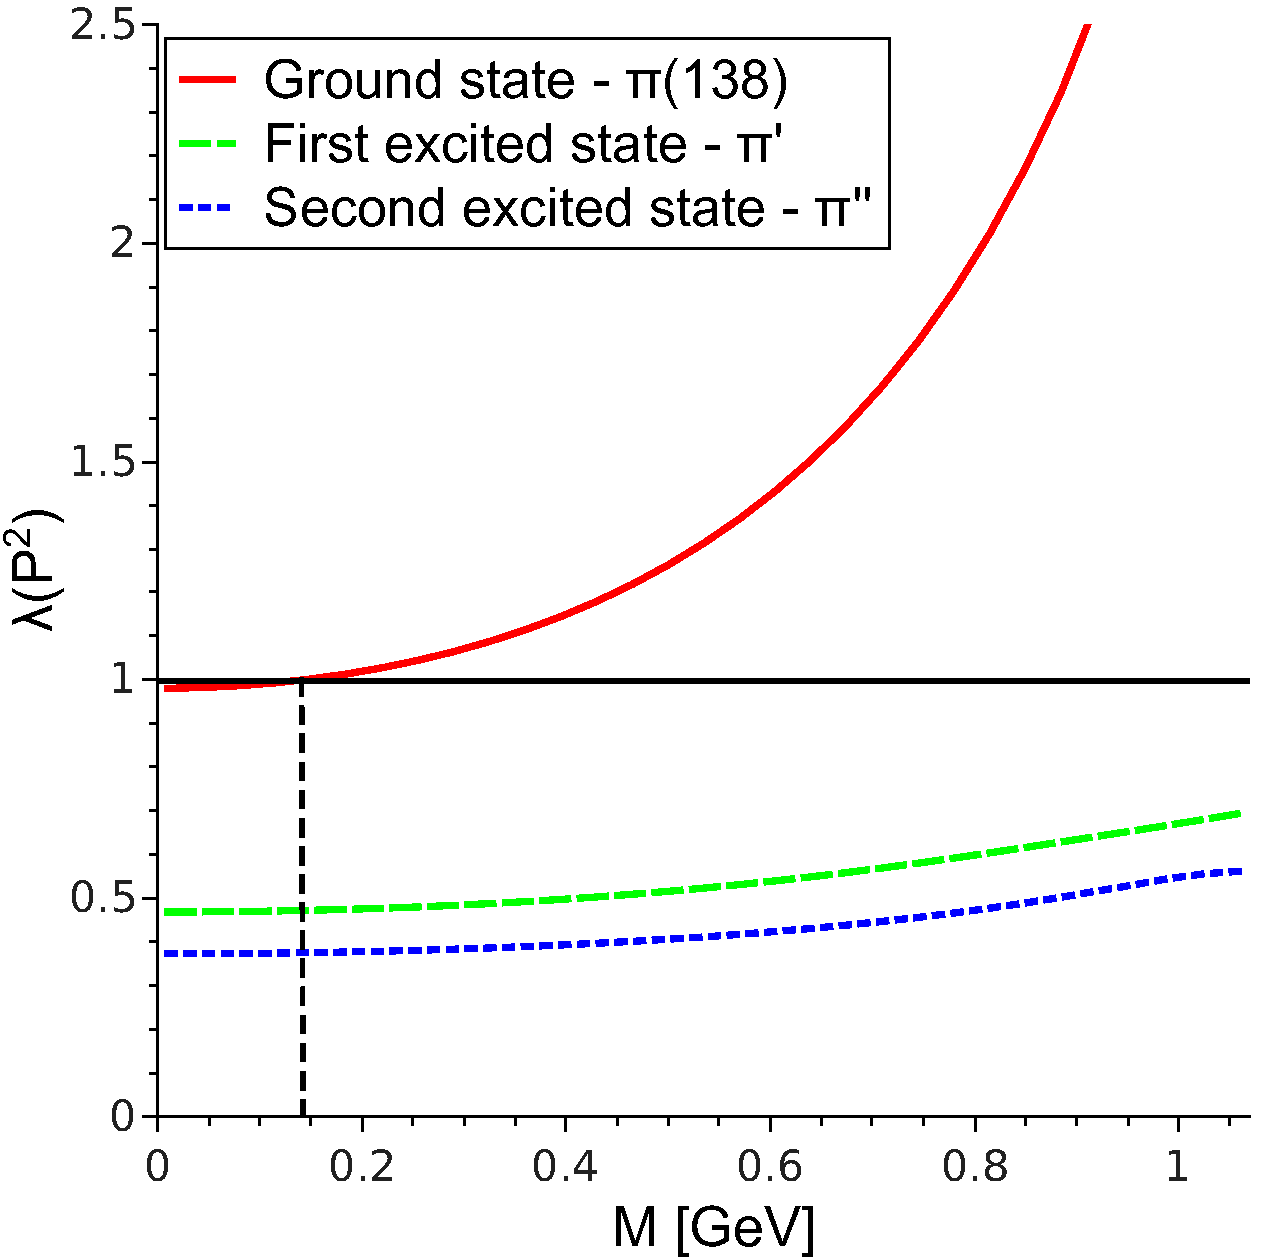
\includegraphics[width=0.49\textwidth]{figures/lambda_pseudo} 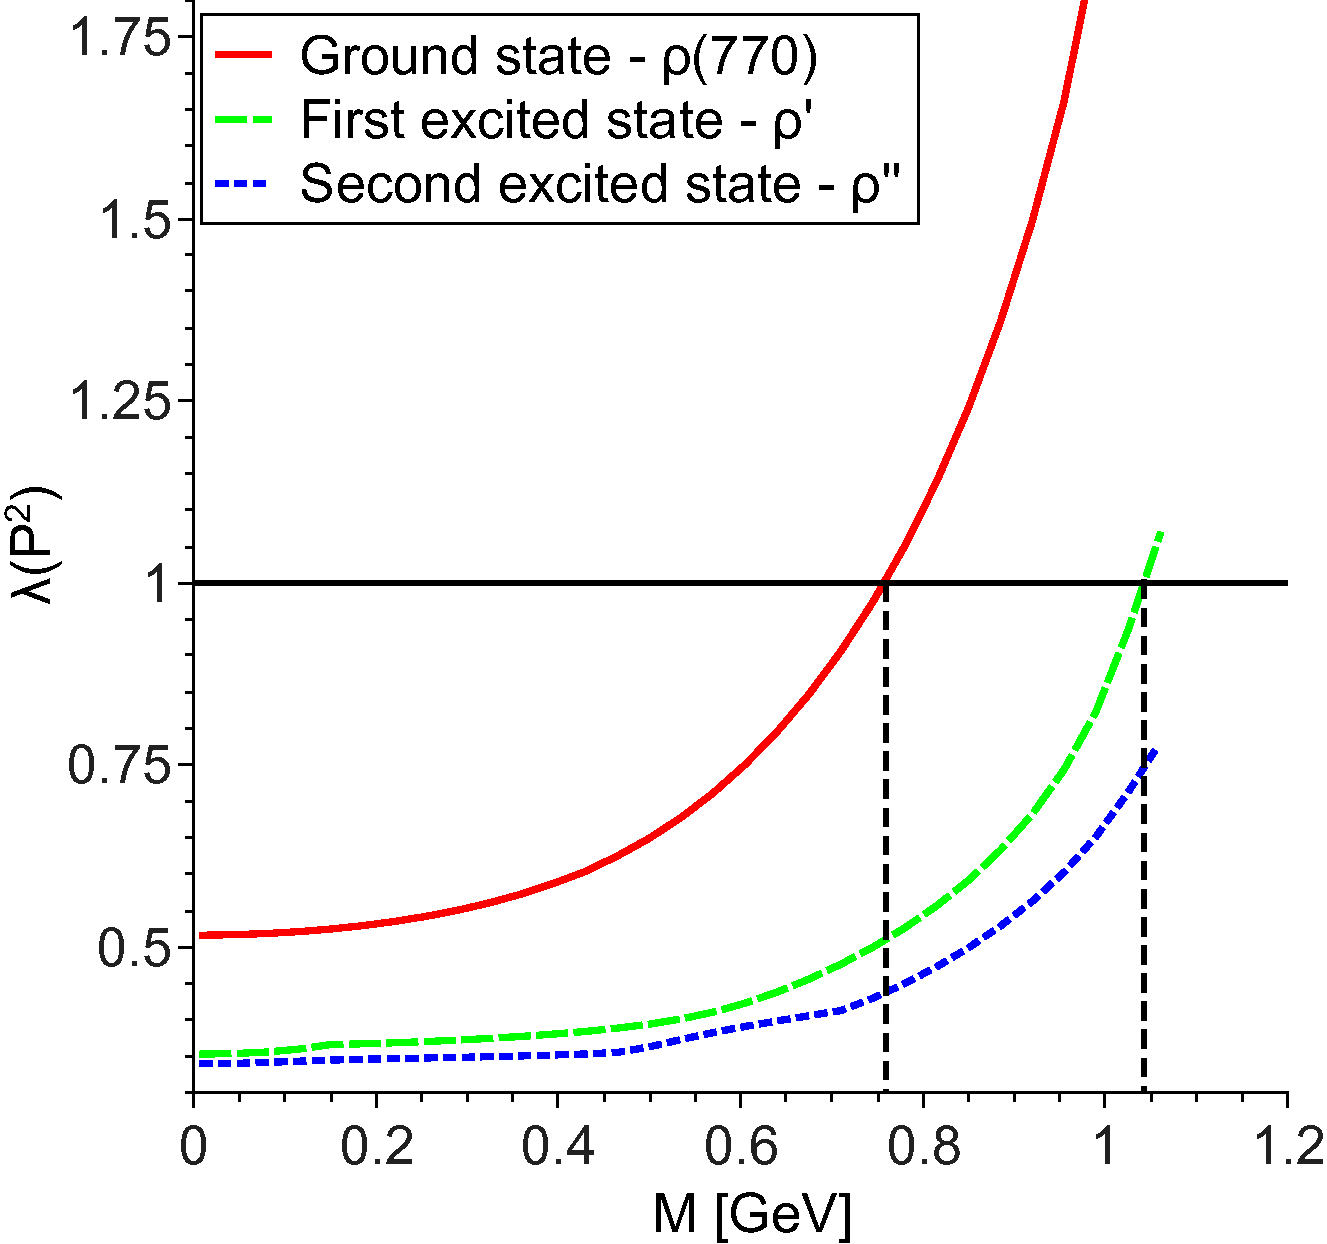
\includegraphics[width=0.49\textwidth]{figures/lambda_vector}
\caption{\footnotesize The behaviour of $\lambda$ in respect to $P^2$ for pion and rho correspondingly.}\label{fig:lambda_pseudo_vector}
\end{center}
\end{figure}
\begin{figure}[H]
\begin{center}
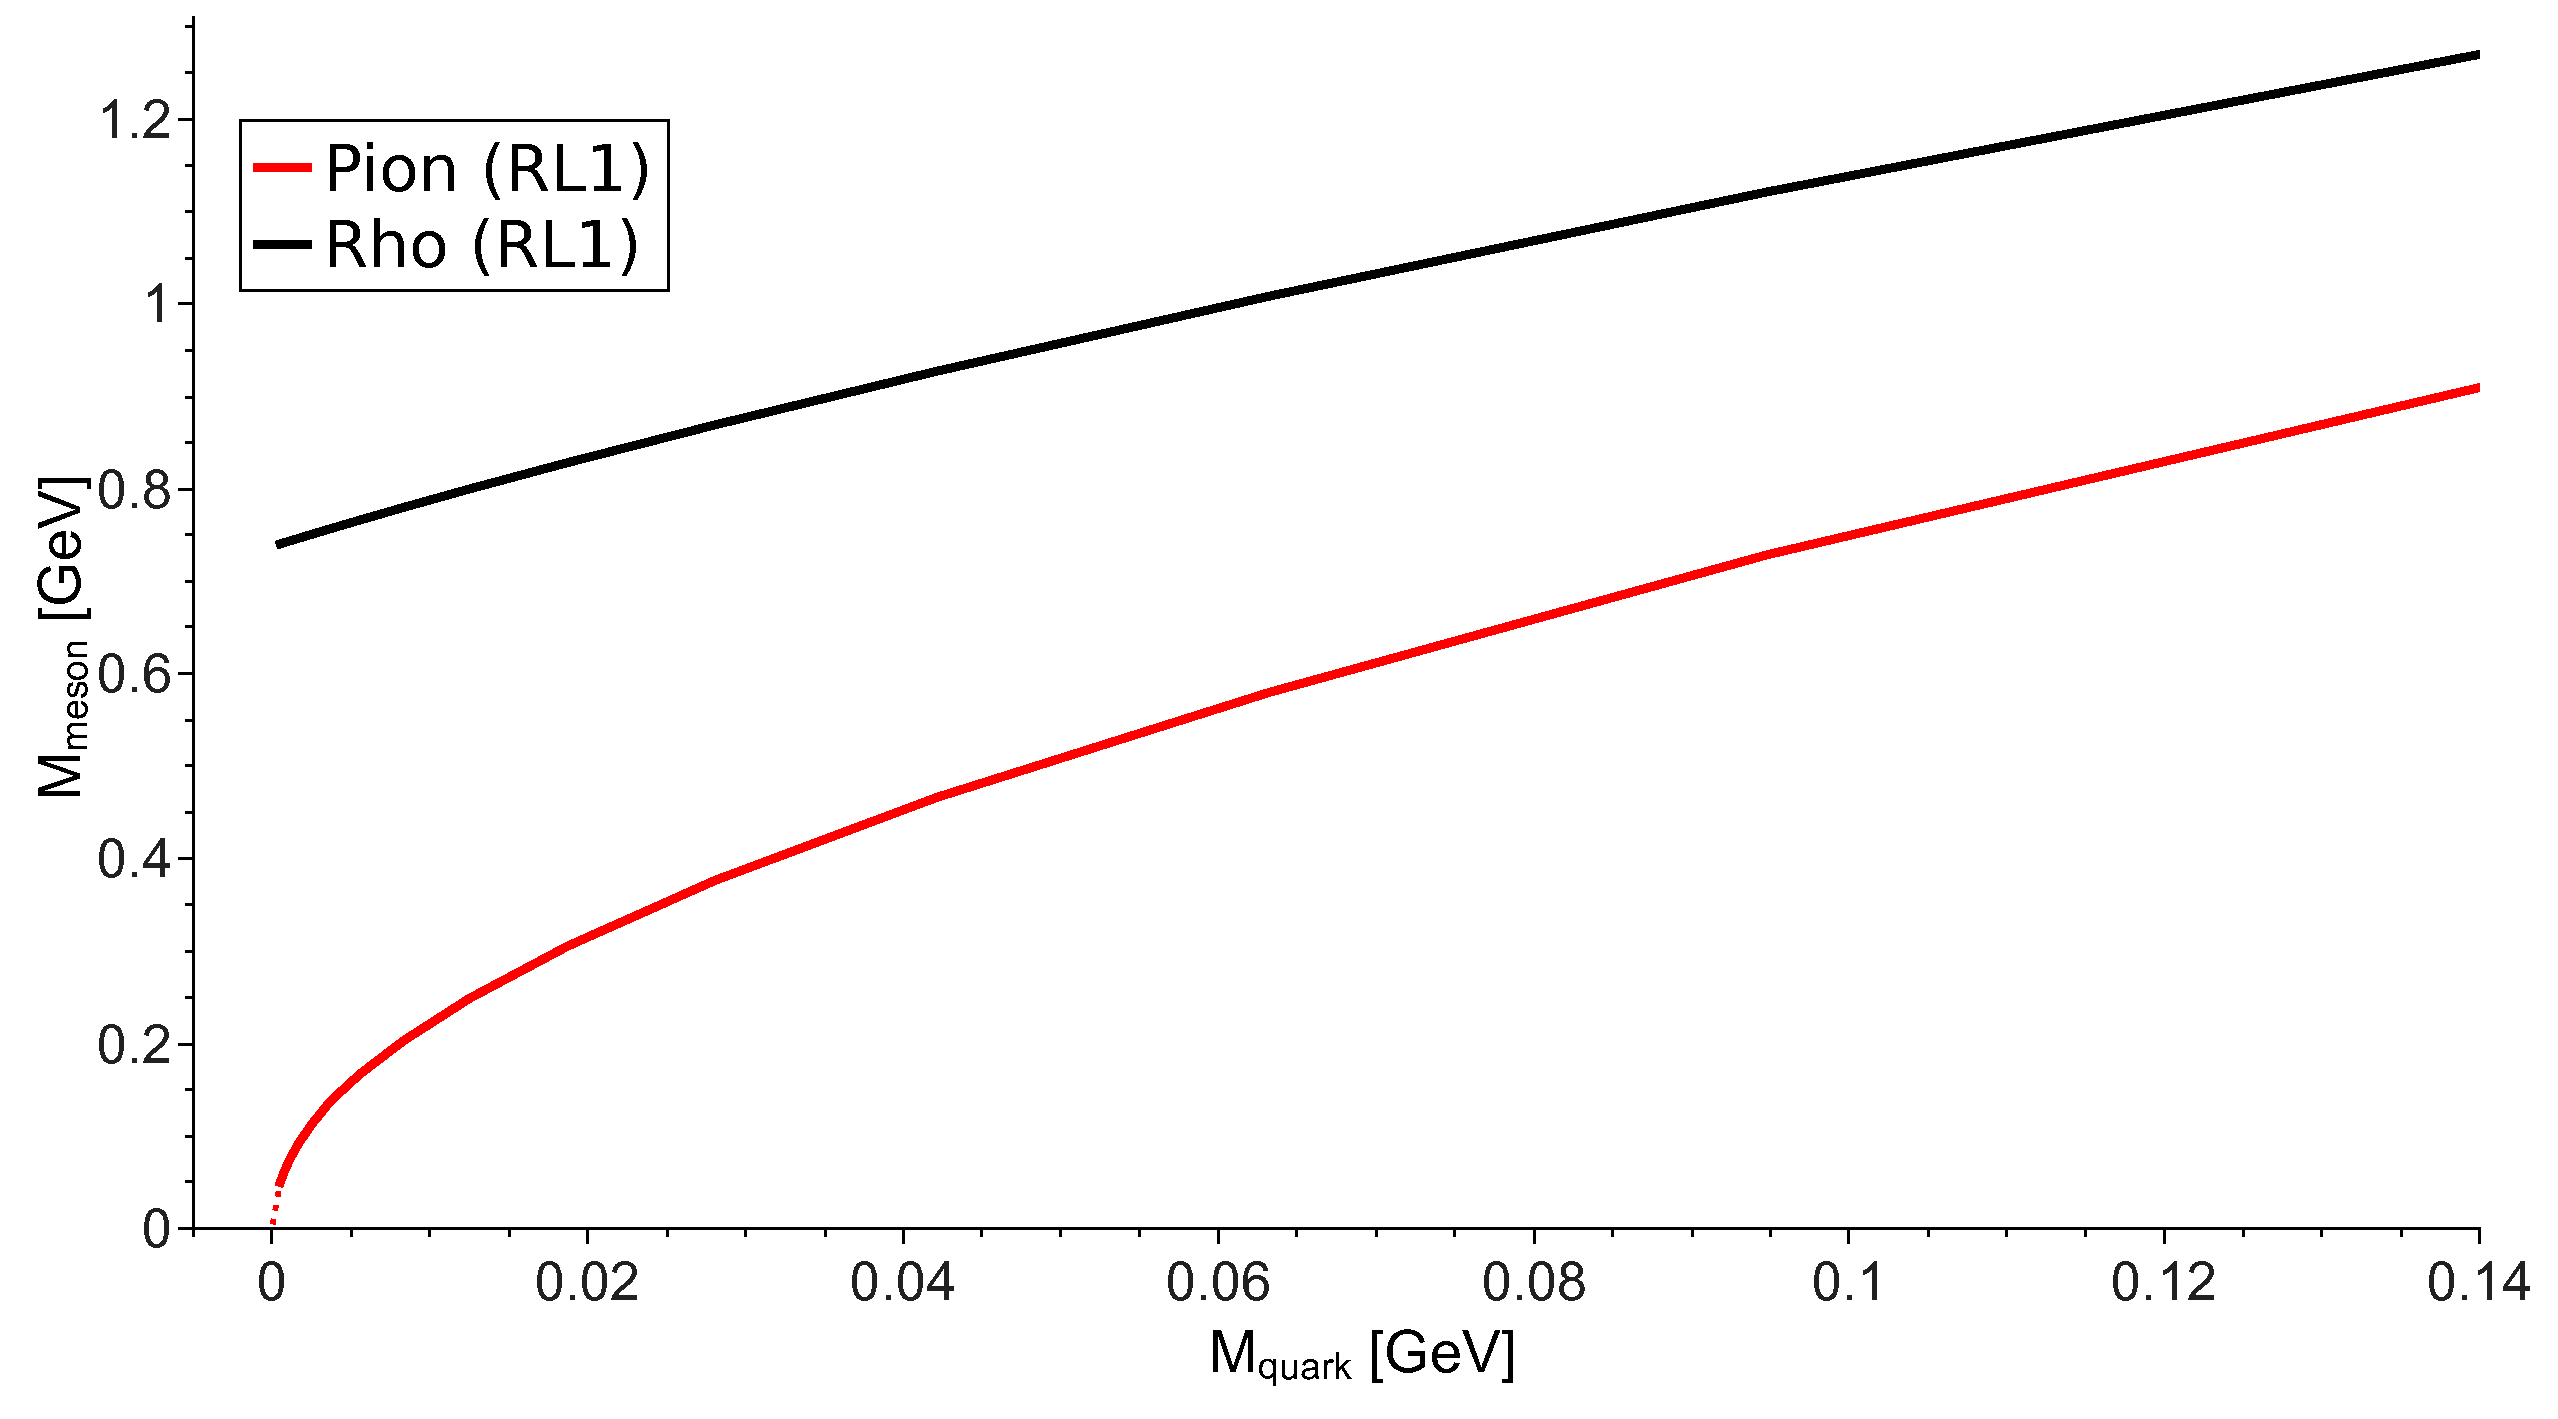
\includegraphics[width=0.99\textwidth]{figures/GMOR_RL} 
\caption{\footnotesize The pion and rho bound states masses as functions of the quark mass. GMOR square root type behaviour for the pion in the vinisity of chiral limit is indicated. }\label{fig:GMOR_RL}
\end{center}
\end{figure} 
\begin{figure}[!]
\begin{center}
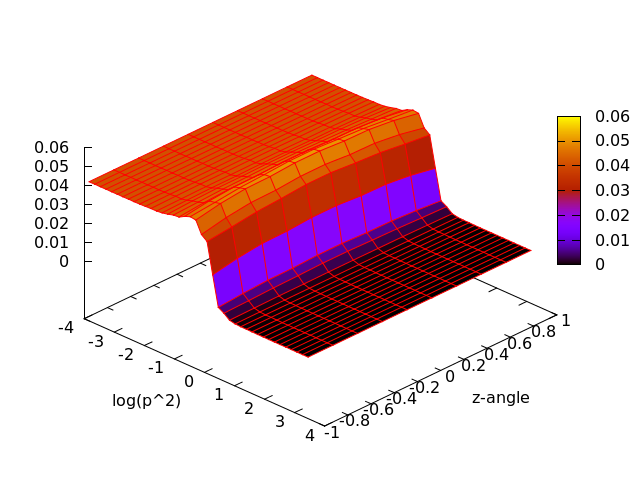
\includegraphics[width=0.80\textwidth]{figures/bsa_vector_ground} 
\caption{\footnotesize The $\gamma^\mu$ component of vector meson \BS amplitude of ground state in respect to $(p^2,z)$ dependence.}\label{fig:bsa_vector_ground}
\end{center}
\end{figure}
\begin{figure}[H]
\begin{center}
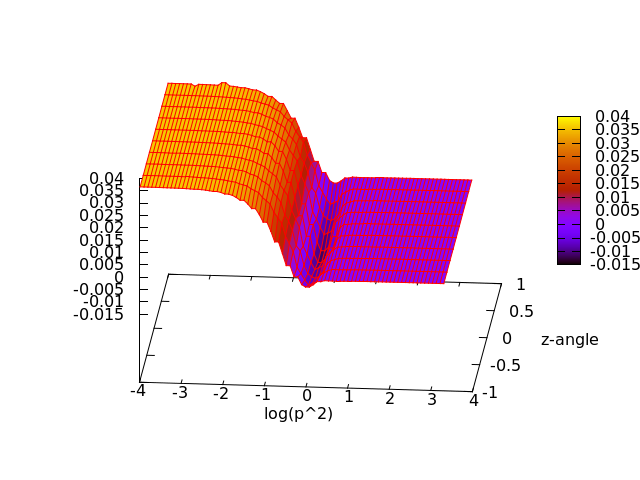
\includegraphics[width=0.80\textwidth]{figures/bsa_vector_excited} 
\caption{\footnotesize The $\gamma^\mu$ component of vector meson \BS amplitude of excited state in respect to $(p^2,z)$ dependence.}\label{fig:bsa_vector_excited}
\end{center}
\end{figure} 
The result of such calculation is a point on the graph $(\lambda(P^2),M)$, where $P^2 = - M^2$. In order to find the mass of meson bound state we search the point where the eigenvalue curve crosses the line $\lambda(P^2)=1$, as it is illustrated on Fig. \ref{fig:lambda_pseudo_vector} for $J^{PC} = 0^{-+}$ pseudoscalar channel and for $J^{PC} = 1^{--}$ vector channel. The employed single gluon rainbow-ladder truncation fulfils GMOR behaviour as it is shown on Fig. \ref{fig:GMOR_RL}. Note that our calculation is not restricted to only ground state, in principal the eigenvalue calculation gives access to the lambda curve of any excited state and the limit how high we search for the state to appear comes only from non-analytical structure of used quark propagator. \\ 

This approach is also beneficial since for every eigenvalue $\lambda$ we can obtain corresponding eigenvector $\mathcal{A}$, and therefore the meson vertex function $\Gamma^{(\mu...)}(p;P)$. As an example the first amplitude of ground state $\rho(770)$ in vector channel is given on Fig. \ref{fig:bsa_vector_ground}, together with the first amplitude of excited state $\rho^\prime$ on Fig. \ref{fig:bsa_vector_excited}. It is apparent that the BSA of excited state expose zero-crossing along the $p^2$ axis. The similar behaviour for meson wave function we can see if we consider the radial excitations within the naive quark model calculation involving Schroedinger equation with Cornell potential. This fact allows us to identify the radial excitations among obtained excited states.
%However it is not the only way to observe a bound state within meson \BSE. The another approach is to consider the off-shell versions of corresponding meson BSEs, given by Eq.(\ref{bse:BSE_inhom}) in form:
%\beqa
%	\Gamma^{(\mu...)}(p;P) = \Gamma^{(\mu...)}_{0}(p;P) + \int_k K(p,k;P)\left[ S(k_+)\Gamma^{(\mu...)}(k;P)S(k_-)\right]\;
%	\label{spectra:BSE_inhom}
%\eeqa
%
\section{Light Quark Meson Spectroscopy}
%
Firstly we consider the \textit{rainbow-ladder} ansatz, where the interaction kernel admits no mixing between states. Furthermore we work in the isospin symmetric limit using equal current quark masses $m_u=m_d=0.0037$ GeV at a renormalization scale of $\mu = 19$ GeV. Since we are in isospin symmetric limit, our calculated meson spectrum is degenerate in the isoscalar/isovector channel for $n=u,d$ quarks. The explicit numbers can be found in Table \ref{tab:results_n&s} and in Table \ref{tab:results_ns}. In Fig.~\ref{fig:spectrumnn} we display the resulting spectrum for $n\bar{n}$ mesons, and compare with the isovector channel from experiment. The input up/down quark masses are fixed such that the experimental mass of the $\pi_0$ is reproduced. The resulting ground state mass in the vector channel is also in good agreement with experiment. This is not true, however, for the scalar and axialvector states as noted frequently before, see e.g. \cite{Watson:2004kd}. Here, the deficiency of the rainbow-ladder truncation is obvious and on the 20-40 \% level. In the scalar channel there is some evidence that the lowest lying nonet may not be identified as simple quark-antiquark states, but may be better described as tetraquarks, see {\it e.g.} \cite{Jaffe:1976ig,Giacosa:2006tf,Ebert:2008id,Parganlija:2012fy,Heupel:2012ua} and Refs. therein. Therefore we compare with the $a_0(1450)$, noting that in rainbow-ladder and without potential mixing with the scalar glueball state there is no hope to reproduce the experimental value. \\

The situation is considerably better for the lowest lying tensor state \cite{Krassnigg:2010mh}, which for the upper value of the considered $\eta$-band is even on the 5 $\%$ level compared to the experimental value. While the other tensor states are again far off, at least where comparison with experiment is possible, the situation is again acceptable for the tensor meson with $J=3$ and $PC=\{--\}$. Its mass of $1528^{+71}_{-184}$~MeV compares well with both the isovector $\rho_3$ of mass $1688.8\pm2.1$~MeV (shown in the figure) and the isoscalar $\omega_3$ of mass $1667\pm4$~MeV with again a deviation on the 5 $\%$ level for the upper range of the $\eta$-band. In contrast, we find no bound state in the $J^{PC}=3^{+-}$-channel, whereas for the $J^{PC}=3^{++}$ state with mass $1510^{+81}_{-100}$~MeV there is no well established experimental counterpart.
The good agreement in states $J^{PC}=1^{--},2^{++},3^{--}$ with experiment can be explained in notions of the (pseudo)-potentials used in the quark model. In this language, what distinguishes these channels from the others is that the non-contact part of the spin-spin interaction 
is vanishing or small: for the hyperfine splitting between the pseudoscalar and vector 
\begin{figure}
\begin{center}
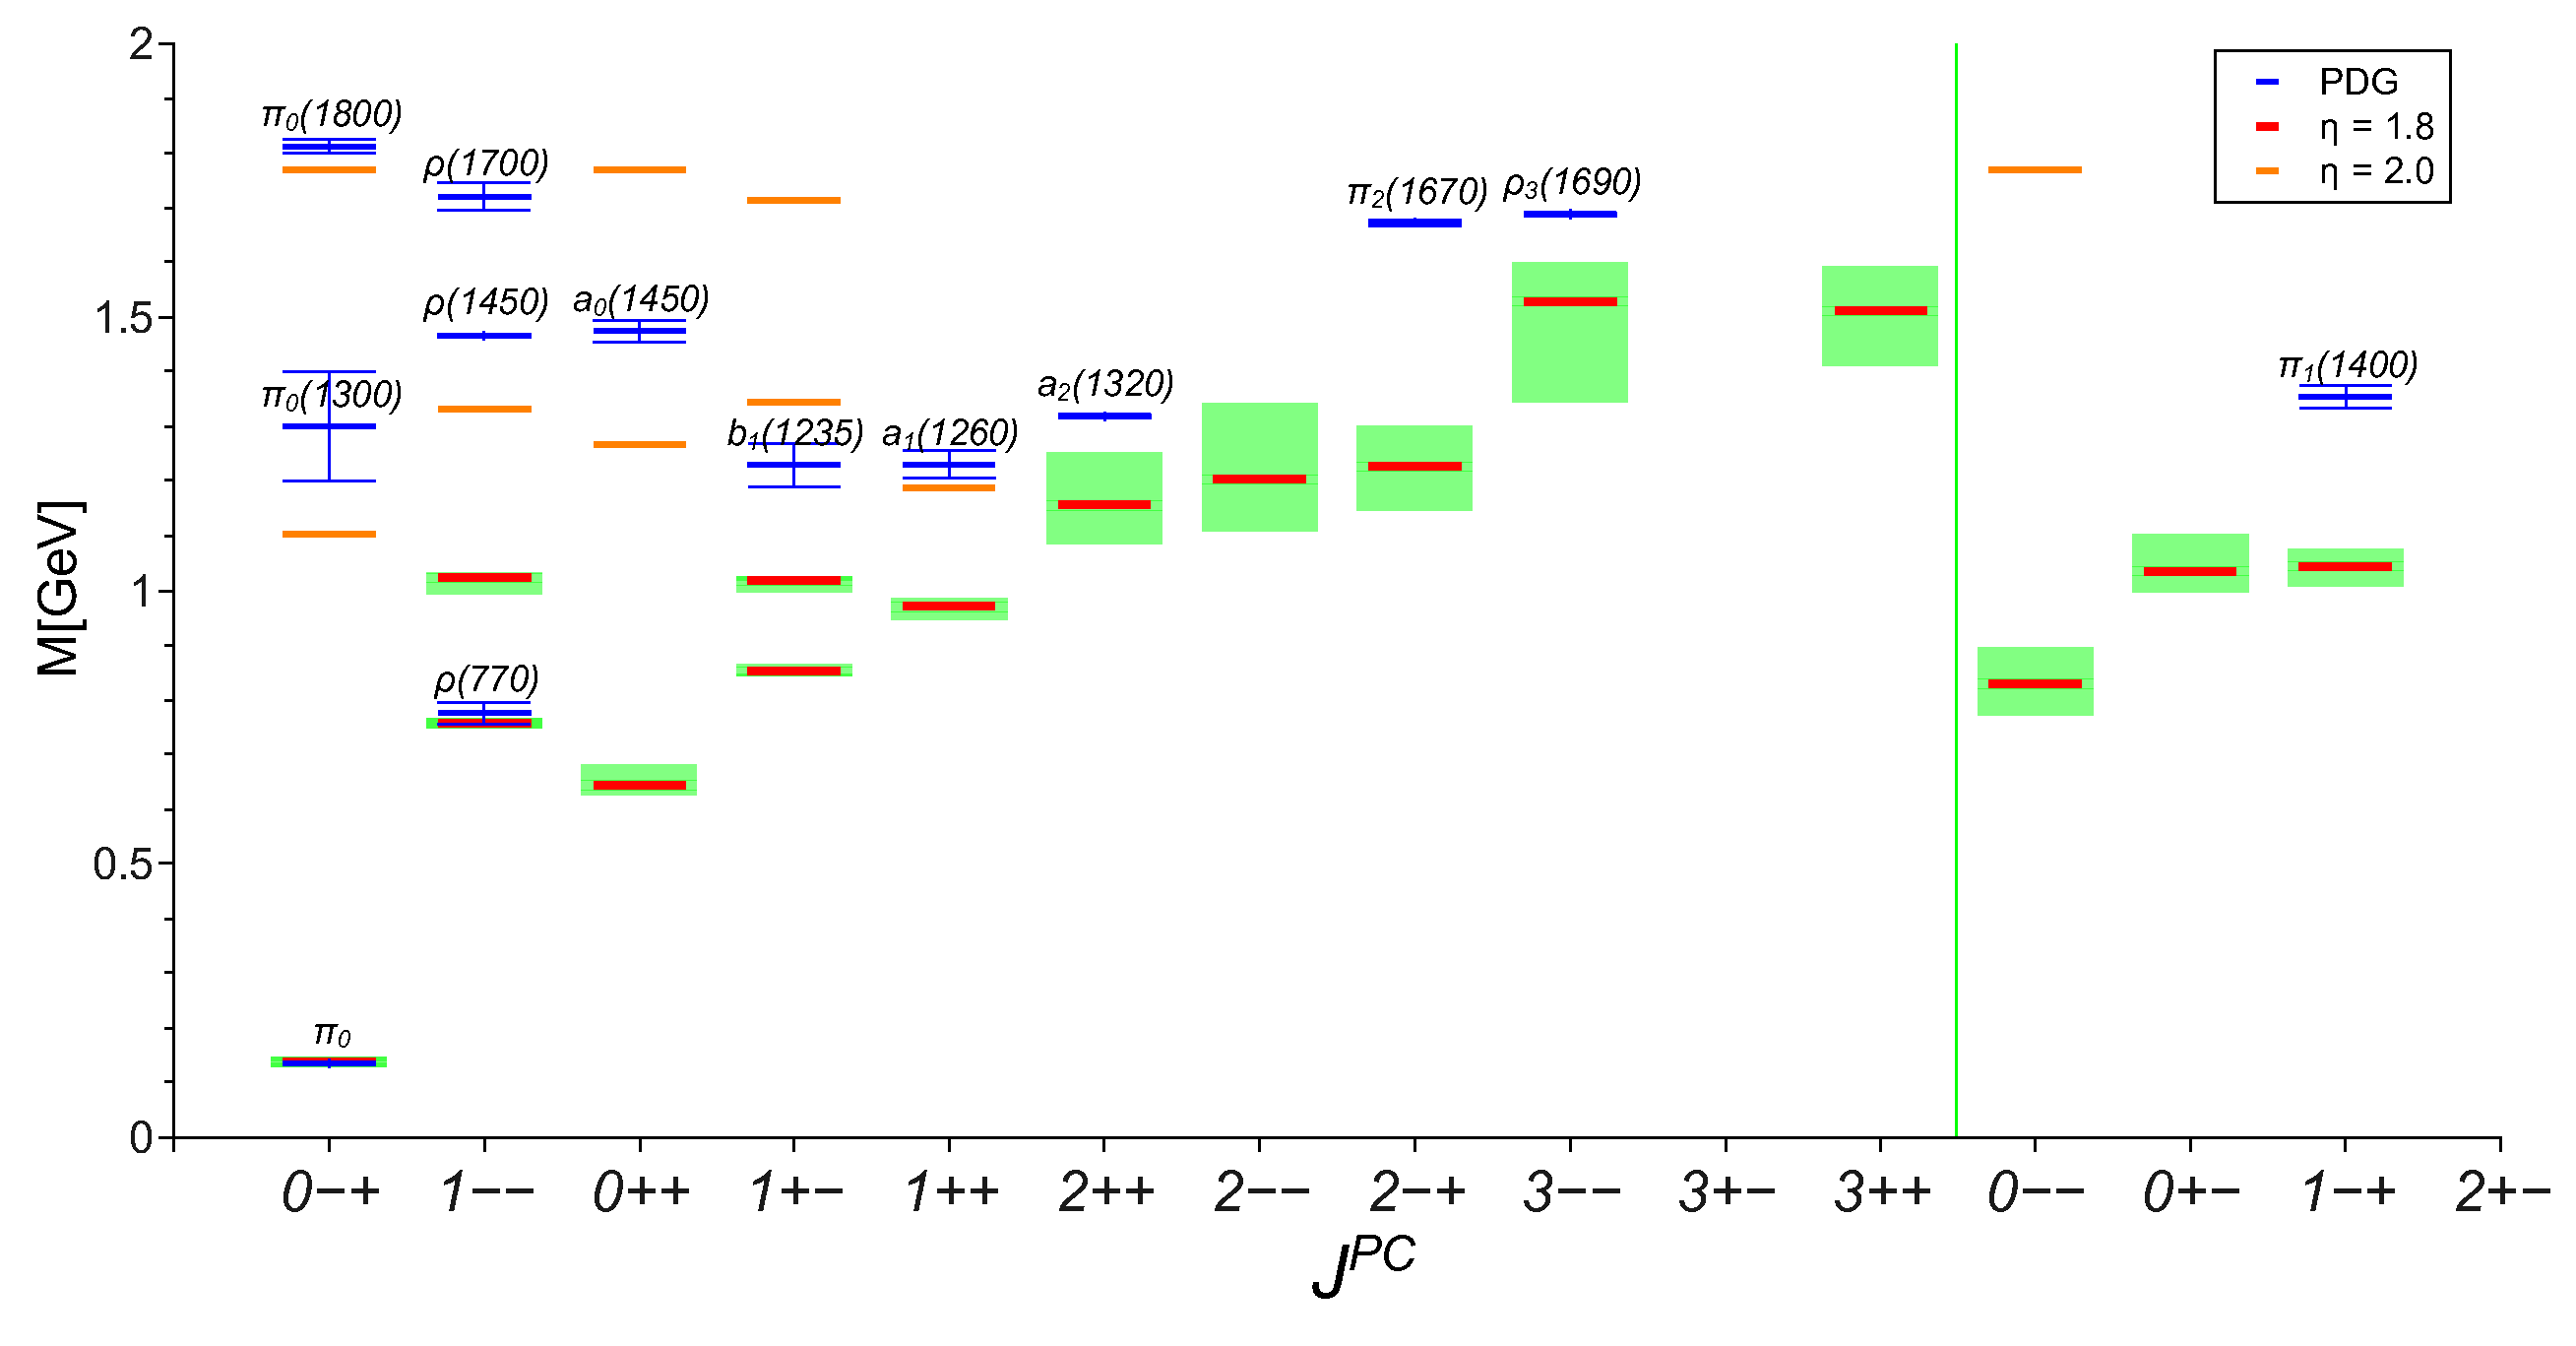
\includegraphics[width=0.999\textwidth]{figures/spectrum_nn}
\caption{\footnotesize The calculated $n\bar{n}$ spectrum, compared to the isovector mesons as measured in 
experiment. The green bands correspond to the 
variation $\eta=1.8\pm0.2$. Due to the structure of the propagator, in the case of $\eta=2.0$ more states are accessible; 
these are given by the single orange lines. The states to the right of the dividing line correspond to exotic quantum 
numbers.}\label{fig:spectrumnn}
\end{center}
\end{figure}
channels the contact part of the spin-spin interaction is dominant, whereas for the $J^{PC}=2^{++},3^{--}$
states the spin-orbit forces prevail. For all other channels considered, there are sizeable 
contributions from the tensor part of the spin-spin interaction. Since these are the channels
that are off, we conclude, that the rainbow-ladder interaction roughly reproduces the size of
the contact part of the spin-spin interaction and the spin-orbit force, but materially overestimates
the binding in the tensor part of the spin-spin interaction. 
\begin{figure*}[t]
\begin{center}
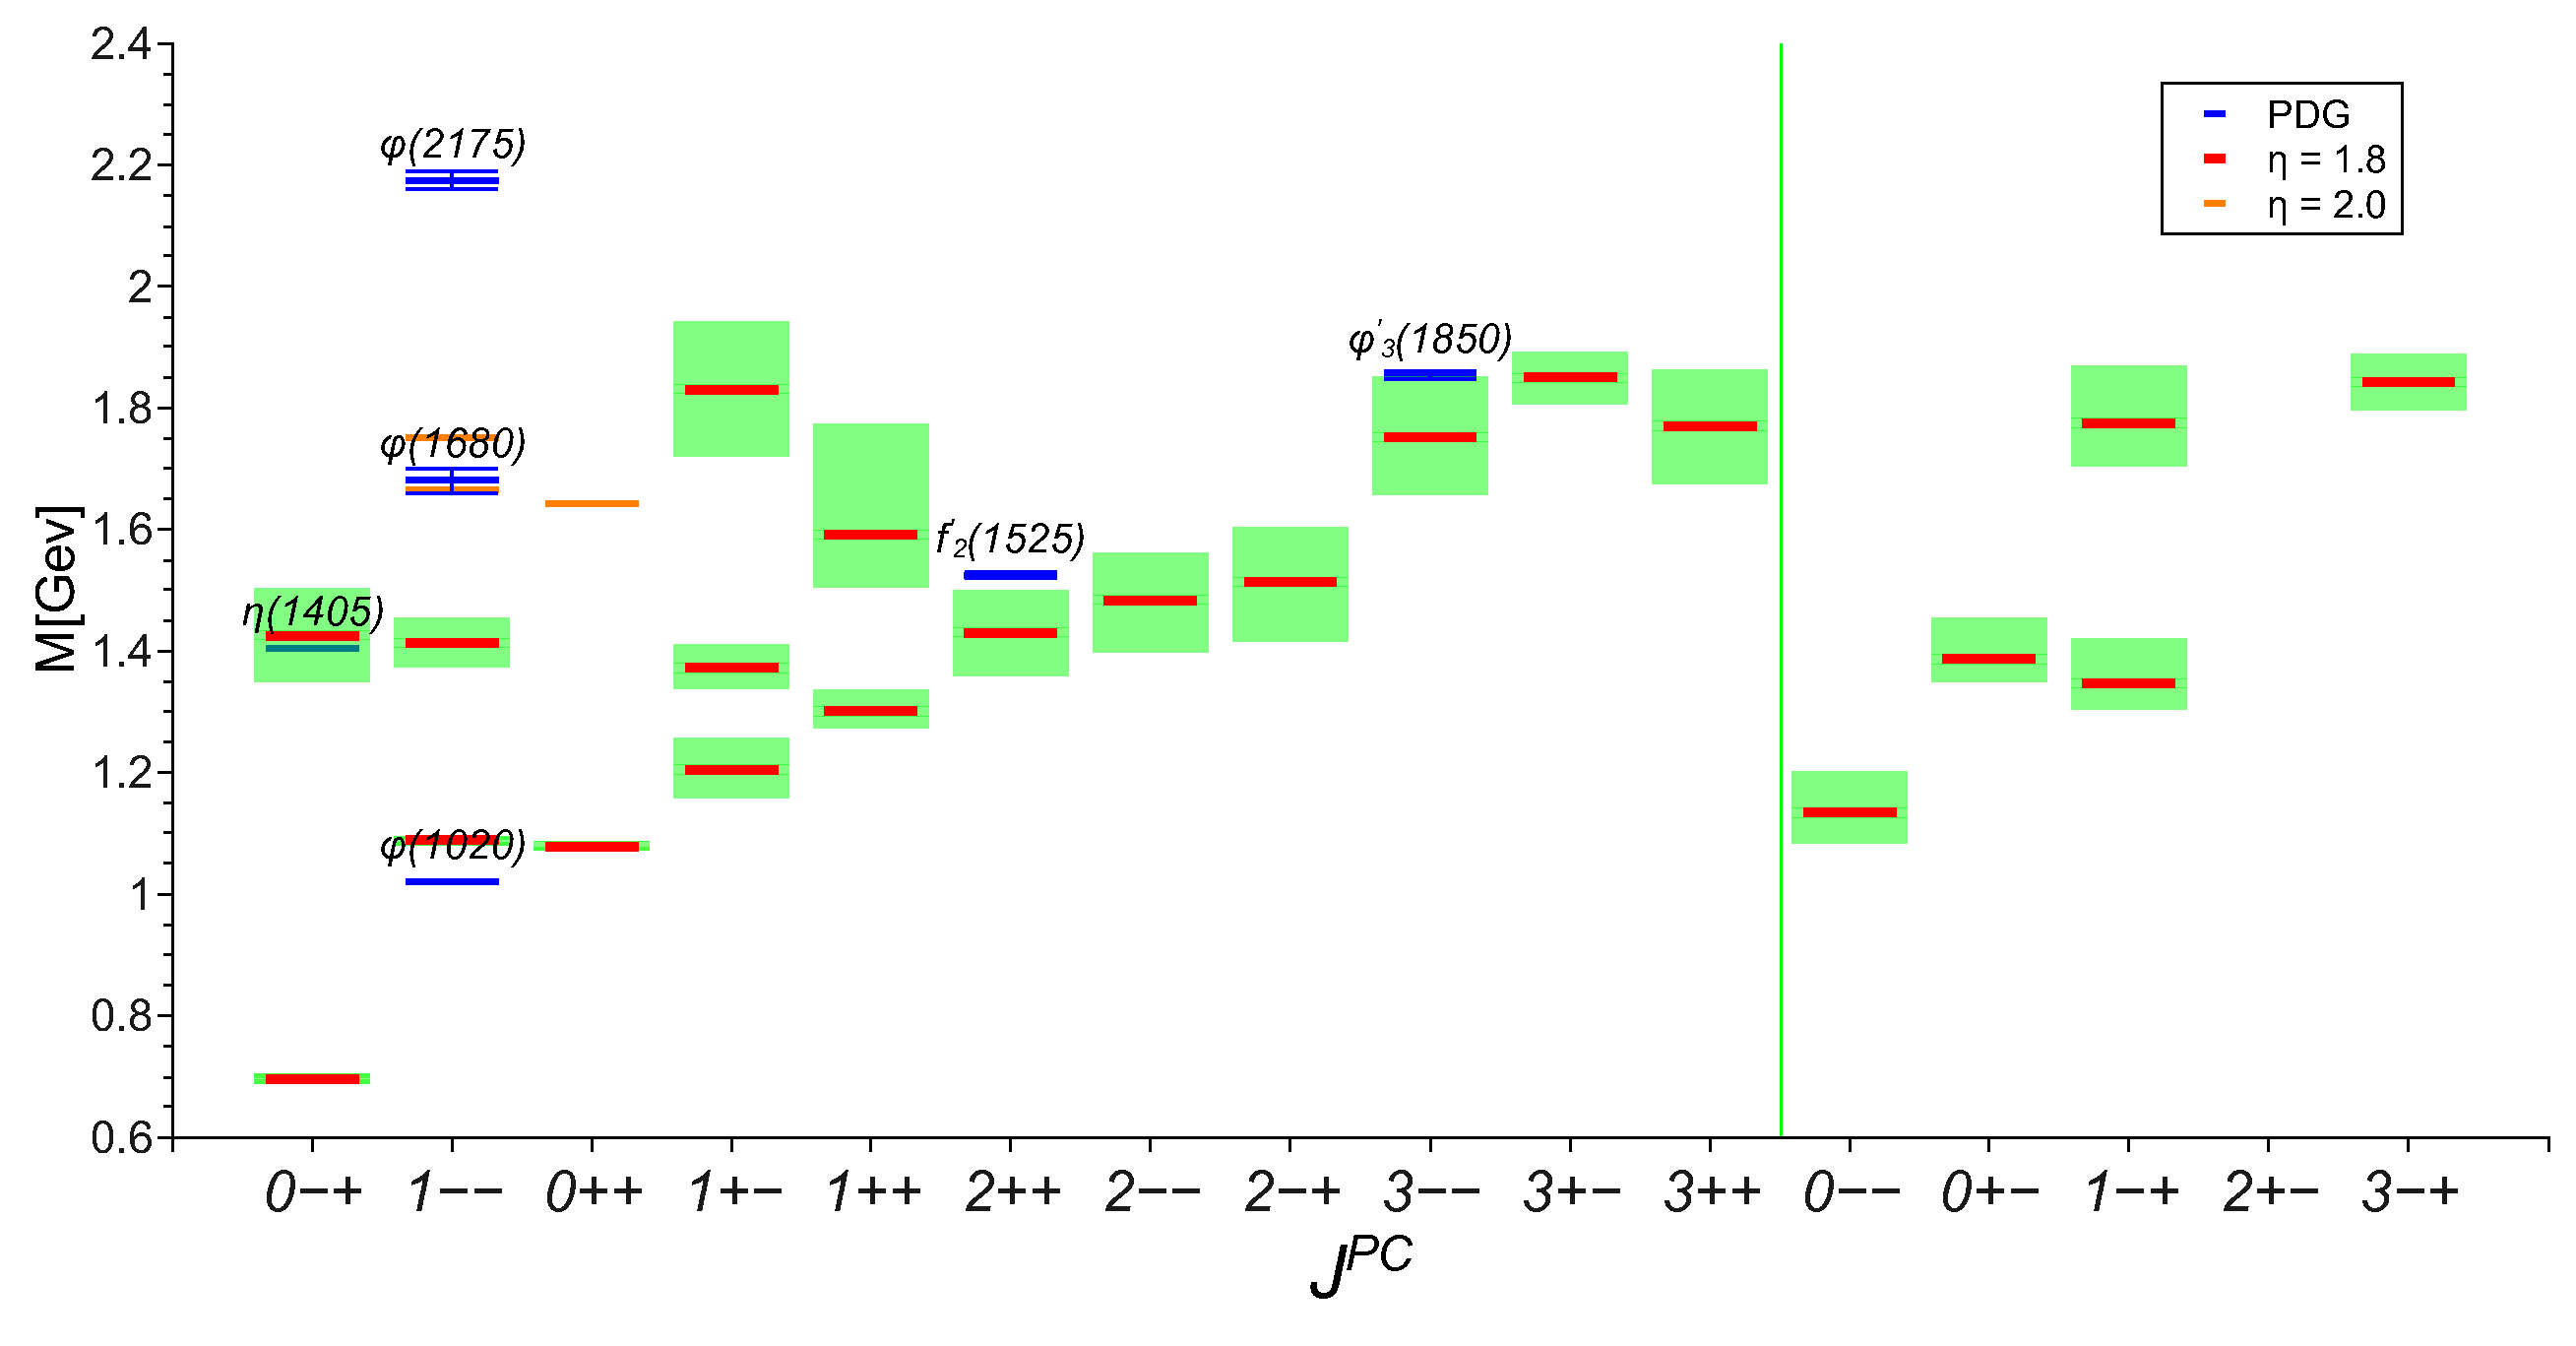
\includegraphics[width=0.999\textwidth]{figures/spectrum_ss}
\caption{ \footnotesize Calculated $s\bar{s}$ spectrum, compared to experiment. The green bands correspond to the 
variation $\eta=1.8\pm0.2$. Due to the structure of the propagator, in the case of $\eta=2.0$ more states are accessible; 
these are given by the single orange lines. The states to the right of the dividing line correspond to exotic quantum 
numbers.}\label{fig:spectrumss}
\end{center}
\end{figure*}\\

As for the exotic channels we find states for $J^{PC}=0^{--},0^{+-}$ with no experimentally established
counterpart, whereas our value for the $J^{PC}=1^{-+}$ is about 25 $\%$ lower than the $\pi_1(1400)$. The physical nature of these exotic states
is yet obscured, indicating the need to extend the effective single gloun exchange model further.
Concerning the excited states, these are in general much too low \cite{Holl:2004fr}
in agreement with the general finding for the ground states. A variation of the $\eta$-value
in general does not improve this picture; also it is noteworthy that higher excited states only
appear for very specific values of $\eta$.  \\

Next we discuss the $s\bar{s}$ spectrum displayed in Fig.~\ref{fig:spectrumss}.
Here the input value of the strange quark mass of $m_s(19 \,\mbox{GeV}) = 0.085$ GeV at the renormalization
point is determined from matching to the experimental value of the kaon mass.
First note that the pseudoscalar $s\bar{s}$-state is too light in this truncation since neither the 
effect of the $U_A(1)$ anomaly (see {\it e.g.} \cite{Alkofer:2008et} for a treatment of the anomaly
in the BSE formalism) nor flavor mixing with the $n\bar{n}$ states is considered. For the excited 
state in the pseudo-scalar channel the surprisingly excellent agreement with the $\eta(1405)$ extracted from
experiment may be accidental. In the vector channel, where mixing effects do not play a major role we
observe good agreement of our bound state mass with experiment. The same is true for the $J^{PC}=2^{++}$
and $J^{PC}=3^{--}$ channels, where the upper boundary of the $\eta$-band almost reproduces the
experimental values for the $f_2(1525)$ and the $\varphi_3(1850)$. Again, these are the channels
with dominating spin-orbit forces in the language of the potential models. In general, the pattern of
states in the $s\bar{s}$ spectrum is very similar to the one found for the $n\bar{n}$ mesons due
to the flavor independence of the underlying rainbow-ladder interaction model. 
\begin{figure*}[t]
\begin{center}
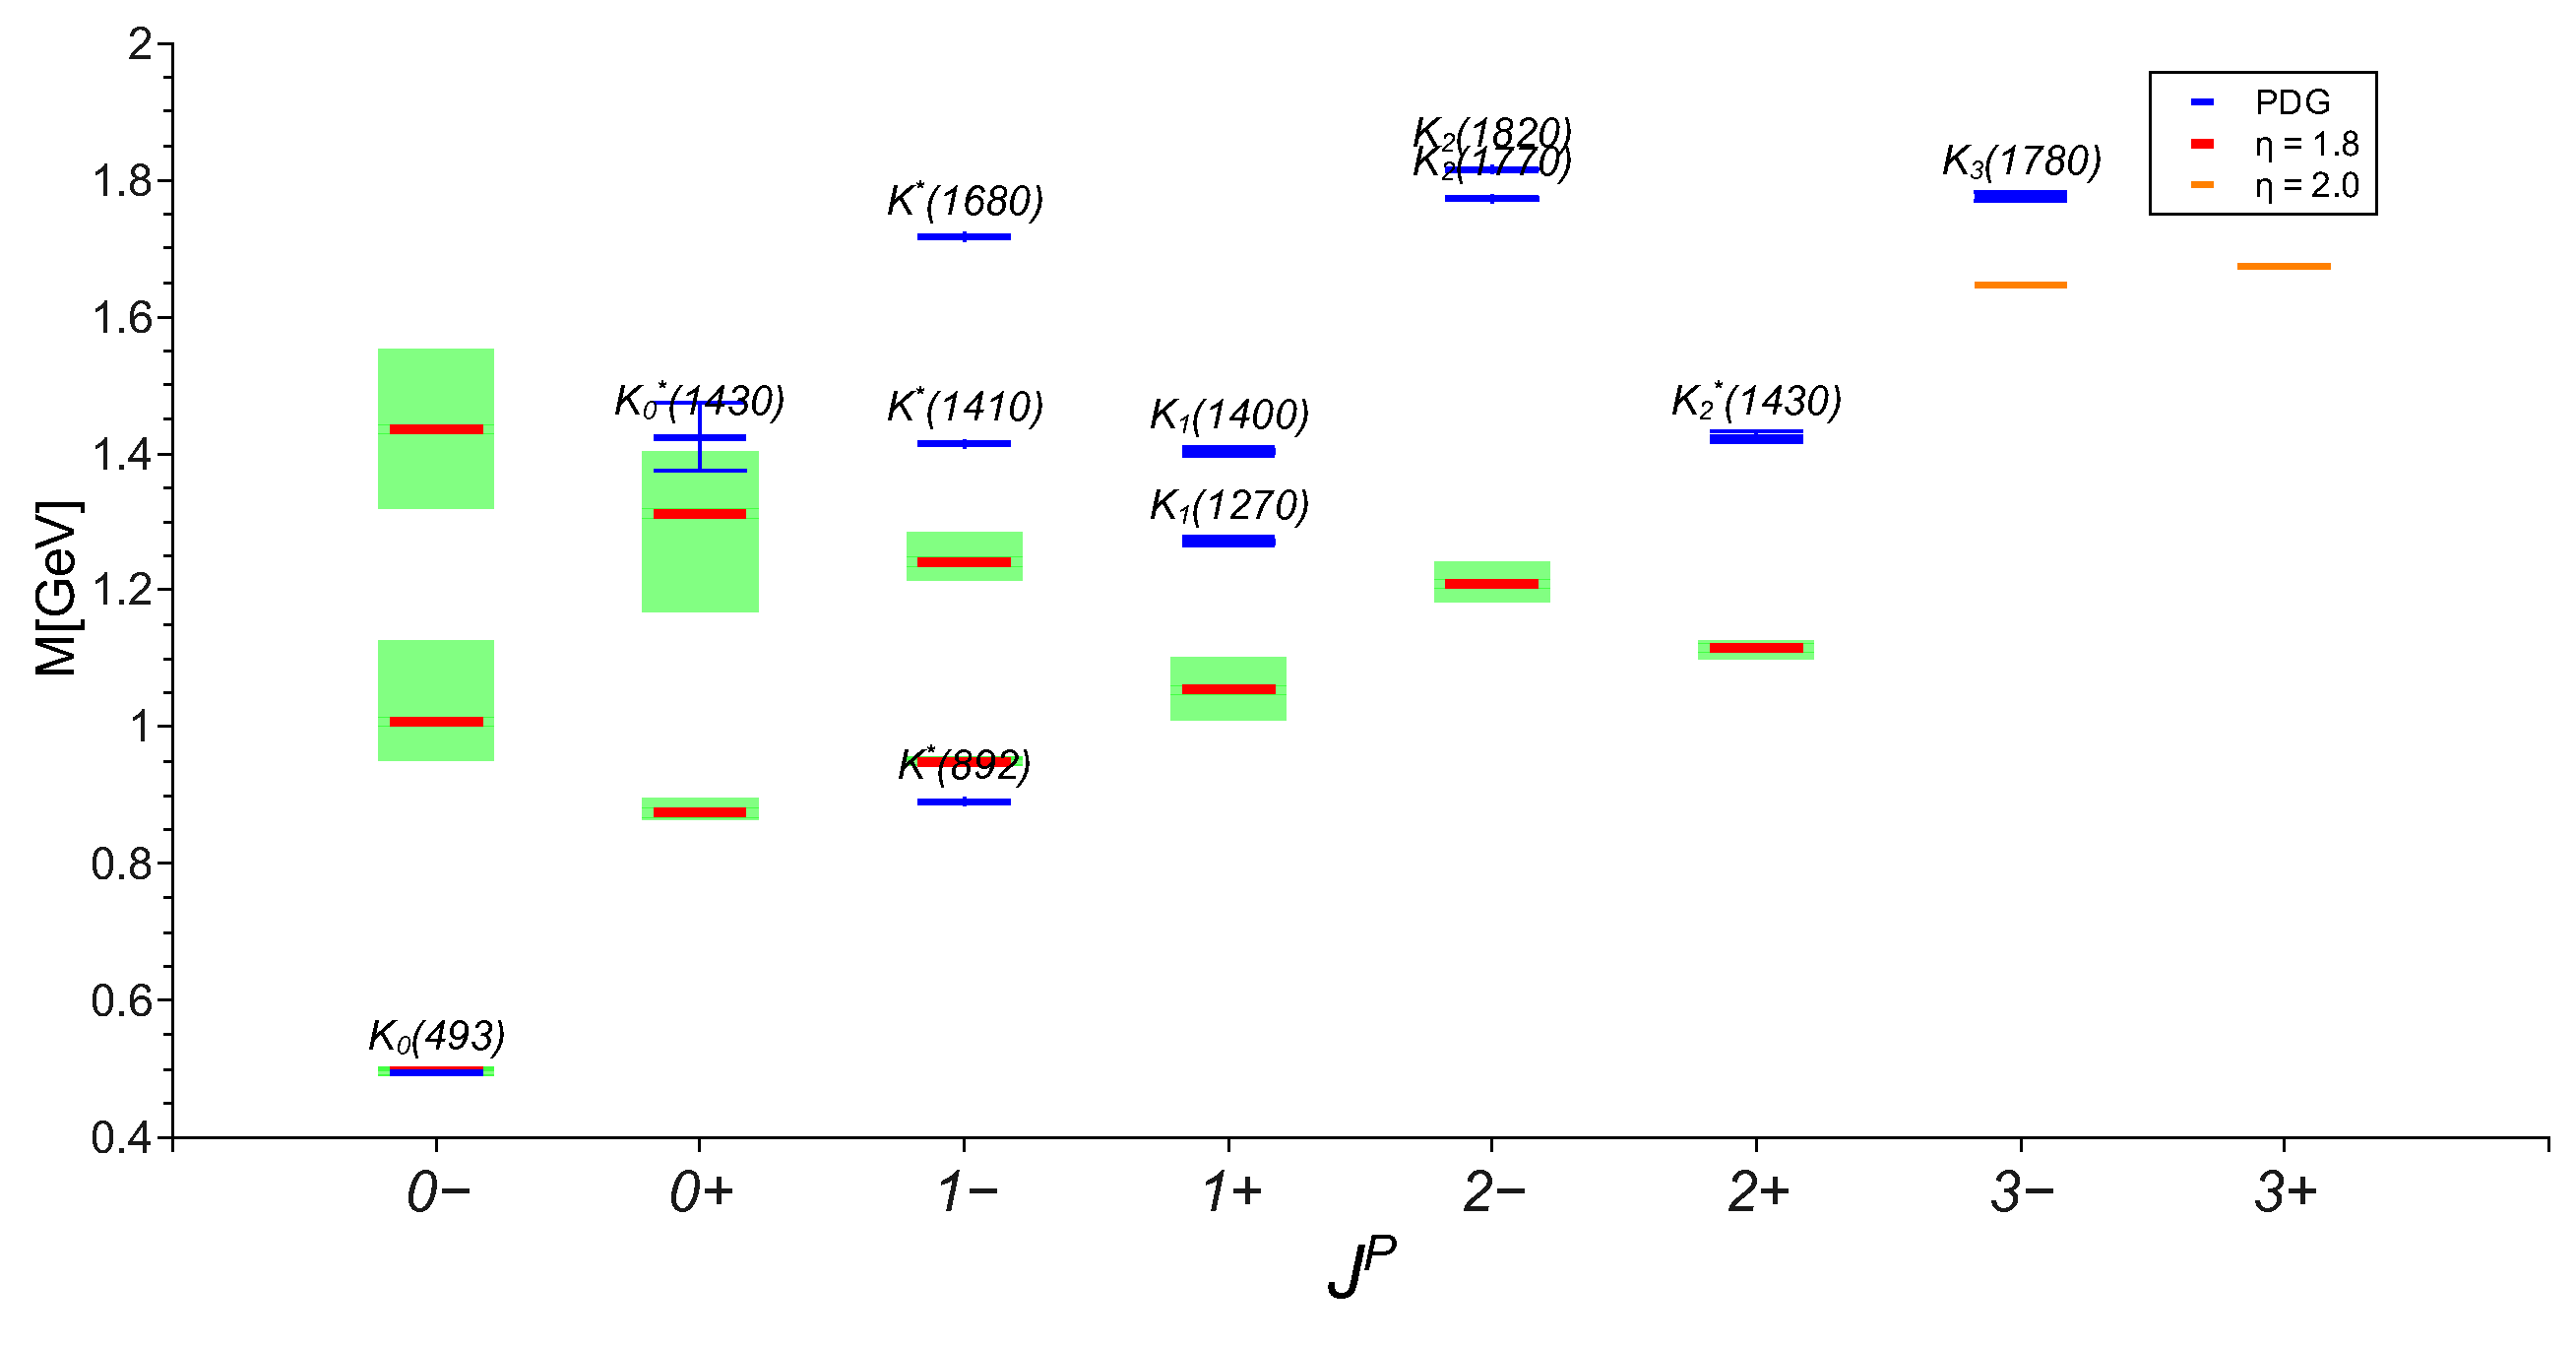
\includegraphics[width=0.999\textwidth]{figures/spectrum_ns}
\caption{\footnotesize Our calculated $n\bar{s}$ spectrum, compared to experiment. The green bands 
correspond to the variation $\eta=1.8\pm0.2$. Due to the structure of the propagator, in the case 
of $\eta=2.0$ more states are accessible; these are given by the single orange lines. The states 
to the right of the dividing line correspond to exotic quantum numbers.
 }\label{fig:spectrumns}
\end{center}
\end{figure*} \\

In the case of strange mesons, $n\bar{s}$, one is no longer able to assign either $C$ or $G$ 
parity to a state. Thus, here there are no states with explicitly exotic quantum numbers.
\begin{table*}[!th]
\renewcommand{\arraystretch}{1.3}
\begin{tabular}{c|ccc|ccc|}
\hline
\hline
                            & \multicolumn{3}{c|}{$n\bar{n}   $}                                                         & \multicolumn{3}{c|}{$s\bar{s}$}  \\
$J^{PC}$                    & $n=0$                                &   $n=1$                            &          $n=2$ & $n=0$                     &   $n=1$                   &          $n=2$    \\
\hline                                                                                                                                                                                                     
$0^{-+}$                    & $138.1^{+1.3}_{-0.6}$                &   $1103.0^\dag$                    &  $1770.1^\dag$ &  $696.3^{+2.4}_{-1.7}$    &  $1426.3_{-76.6}$         &                   \\
$0^{--}$                    & $828.8^{+66.9}_{-57.1}$              &                                    &                &  $1133.8^{+68.0}_{-50.8}$ &                           &                   \\
$0^{++}$                    & $643.6^{+17.6}_{-37.6}$              &   $1266.9^\dag$                    &  $1769.1^\dag$ &  $1079.4^{+1.7}_{-7.9}$   &  $1643.6^\dag$            &                   \\
$0^{+-}$                    & $1035.5^{+66.8}_{-38.8}$             &                                    &                &  $1386.7^{+68.8}_{-37.9}$ &                           &                   \\
\hline                                                                                                                                                                                                     
$1^{-+}$                    & $1043.9_{-37.0}$                     &                                    &                &  $1347.3^{+73.2}_{-43.7}$ &  $1870.1^{\ddag}$         &                   \\
$1^{--}$                    & $757.2^{+1.2}_{-0.6}$                & $1022.6^{+\phantom{1}9.2}_{-29.2}$ & $1331.9^\dag$  &  $1087.8^{+1.8}_{-2.2}$   &  $1413.1^{+38.8}_{-42.1}$ &   $1666.9^\dag$   \\                                                                                                                                                                       
$1^{++}$                    & $969.4^{+15.6}_{-23.9}$              & $1188.1^\dag$                      &                &  $1301.0^{+34.7}_{-28.5}$ &  $1591.9^{+181.2}$        &                   \\
$1^{+-}$                    & $852.1^{+13.6}_{-\phantom{1}5.2}$    & $1017.4^{+\phantom{1}0.6}_{-21.4}$ & $1345.2^\dag$  &  $1205.1^{+51.8}_{-46.6}$ &  $1372.0^{+34.4}_{-39.5}$ &   $1831.6^\dag$   \\
\hline                                                                                                                                                                                                     
$2^{-+}$                    & $1226.5^{+73.9}_{-80.0}$             &                                    &                &  $1513.5^{+90.5}_{-85.0}$ &                           &                   \\
$2^{--}$                    & $1202.6^{+140.0}_{-\phantom{1}94.3}$ &                                    &                &  $1484.7^{+76.0}_{-86.0}$ &                           &                   \\
$2^{++}$                    & $1154.8^{+96.5}_{-69.3}$             &                                    &                &  $1431.4^{+72.4}_{-69.3}$ &                           &                   \\
$2^{+-}$                    &                                      &                                    &                &                           &                           &                   \\
\hline                                                                                                                                                                                                     
$3^{-+}$                    &                                      &                                    &                &  $1842.5_{-46.6}$         &                           &                   \\
$3^{--}$                    & $1528.3^{+\phantom{1}71.2}_{-184.2}$ &                                    &                &  $1751.7^{+99.2}_{-94.3}$ &                           &                   \\
$3^{++}$                    & $1510.5^{+\phantom{1}81.6}_{-100.3}$ &                                    &                &  $1770.9^{+91.4}_{-96.1}$ &                           &                   \\
$3^{+-}$                    &  								   		&                                    &                &  $1849.4_{-43.6}$ 		   &                      	     &           			\\                                                                                                                                                                      
\hline
\hline
\end{tabular}
\caption{Mass spectrum in MeV for isospin degenerate $n\bar{n}$ and isoscalar $s\bar{s}$ bound-states. The rainbow-ladder result corresponds to $\eta=1.8\pm0.2$, with the 
superscript ${}^\dag$ (${}^\ddag$) indicating $\eta=2.0$ ($\eta=1.6$) only.}\label{tab:results_n&s}
\end{table*}
The spectrum, as calculated within the rainbow-ladder approximation, is given in Fig.~\ref{fig:spectrumns}. 
As already mentioned above, the strange quark mass is chosen such that the calculated $K^{0,\pm}$ 
is in agreement in experiment; the remaining spectrum is a result of the model.
While the vector ground state is in reasonable agreement with experiment, the remaining spectrum 
does not fare so well (as in the unflavored case).
\begin{table*}
\centering
\renewcommand{\arraystretch}{1.3}
\begin{tabular}{c|ccc|}
\hline
\hline
          				     & \multicolumn{3}{c|}{$n\bar{s}$}  \\
$J^P   $&  $n=0$    &$n=1$  & $n=2$ \\
\hline                                                                                                                                                                                                     
{$0^-$}       &   { $496.6^{+5.3}_{-0.9}$} &  {$1007.6^{+118.3}_{-\phantom{1}57.0}$ } & {$1435.9$} \\                                                                                                                                                                        
{$0^+$}       &  { $874.5^{+10.0}_{-22.2}$ } &  {$1312.5^{+\phantom{1}90.3}_{-143.8}$} &  \\                                                                                                                                                                        
\hline                                                                                                                                                                                                     
{$1^-$}       &   {$ 950.1^{+5.5}_{-1.6}$} &  {$1241.6^{+43.5}_{-27.9}$ } &  \\                                                                                                                                                                  
{$1^+$}       & {$1054.1^{+48.7}_{-44.8}$} &   &  \\
\hline                                                                                                                                                                                                     
{$2^-$}       &  { $1116.2^{+10.9}_{-17.2}$ } &   &  \\
{$2^+$}       &  {$1209.4^{+32.3}_{-26.6}$} &   &  \\
\hline                                                                                                                                                                                                     
{$3^-$}       & { $1646.9^\dag$ }  &   &  \\
{$3^+$}       & { $1673.4^\dag$  } &   &  \\                                                                                                                                                                  
\hline
\hline
\end{tabular}
\caption{Mass spectrum in MeV for $I=1/2$ $n\bar{s}$ bound-states. The rainbow-ladder result corresponds to $\eta=1.8\pm0.2$, with the 
superscript ${}^\dag$ (${}^\ddag$) indicating $\eta=2.0$ ($\eta=1.6$) only.}\label{tab:results_ns}
\end{table*}
Along with the usual $J=1$ and $J=2$ mesons, we find two states with $J=3$, one with positive 
and one with negative parity. For the latter, we have a mass of $1646.9$ (found for $\eta=2.0$ only) 
which compares well with the experimentally known $K_3^\star$ whose mass $1776\pm7$ is within $10\%$. 
The positive parity state is similar in mass, $1673.4$, but the $K_3$ has not been seen in 
experiment. The results strongly indicate that the $n\bar{s}$ system should be investigated in a beyond rainbow-ladder 
approximation, in order to find stronger agreement for the majority of low-lying states. 

\section{Heavy Quark Meson Spectroscopy}
\subsection*{Charmonia}
\label{sec:charm}
%
%
%
%
%
%
We approach the study of heavy quark 2-body systems within rainbow-ladder Truncation using the vanilla Maris-Tandy interaction,
i.e. we keep the scale $\Lambda=0.72$ from the light meson sector and
explore the dependence of the spectrum on $\eta$.

Since $J^{PC}=1^{--},2^{++},3^{--}$ states are well represented in the vanilla
Maris-Tandy (MT) interaction in the light meson sector, we first concentrate
on the ground and first excited states in the $1^{--}$ and $2^{++}$-channels
and explore the variation of the corresponding masses with the charm quark
mass and the $\eta$-parameter in the MT-interaction. We obtained good
agreement with experiment using a charm quark mass of 
$m(19 \,\mbox{GeV}) = 0.870 \,\mbox{GeV}$ and a value $\eta=1.157$.
\begin{figure*}[h]
  \begin{center}
  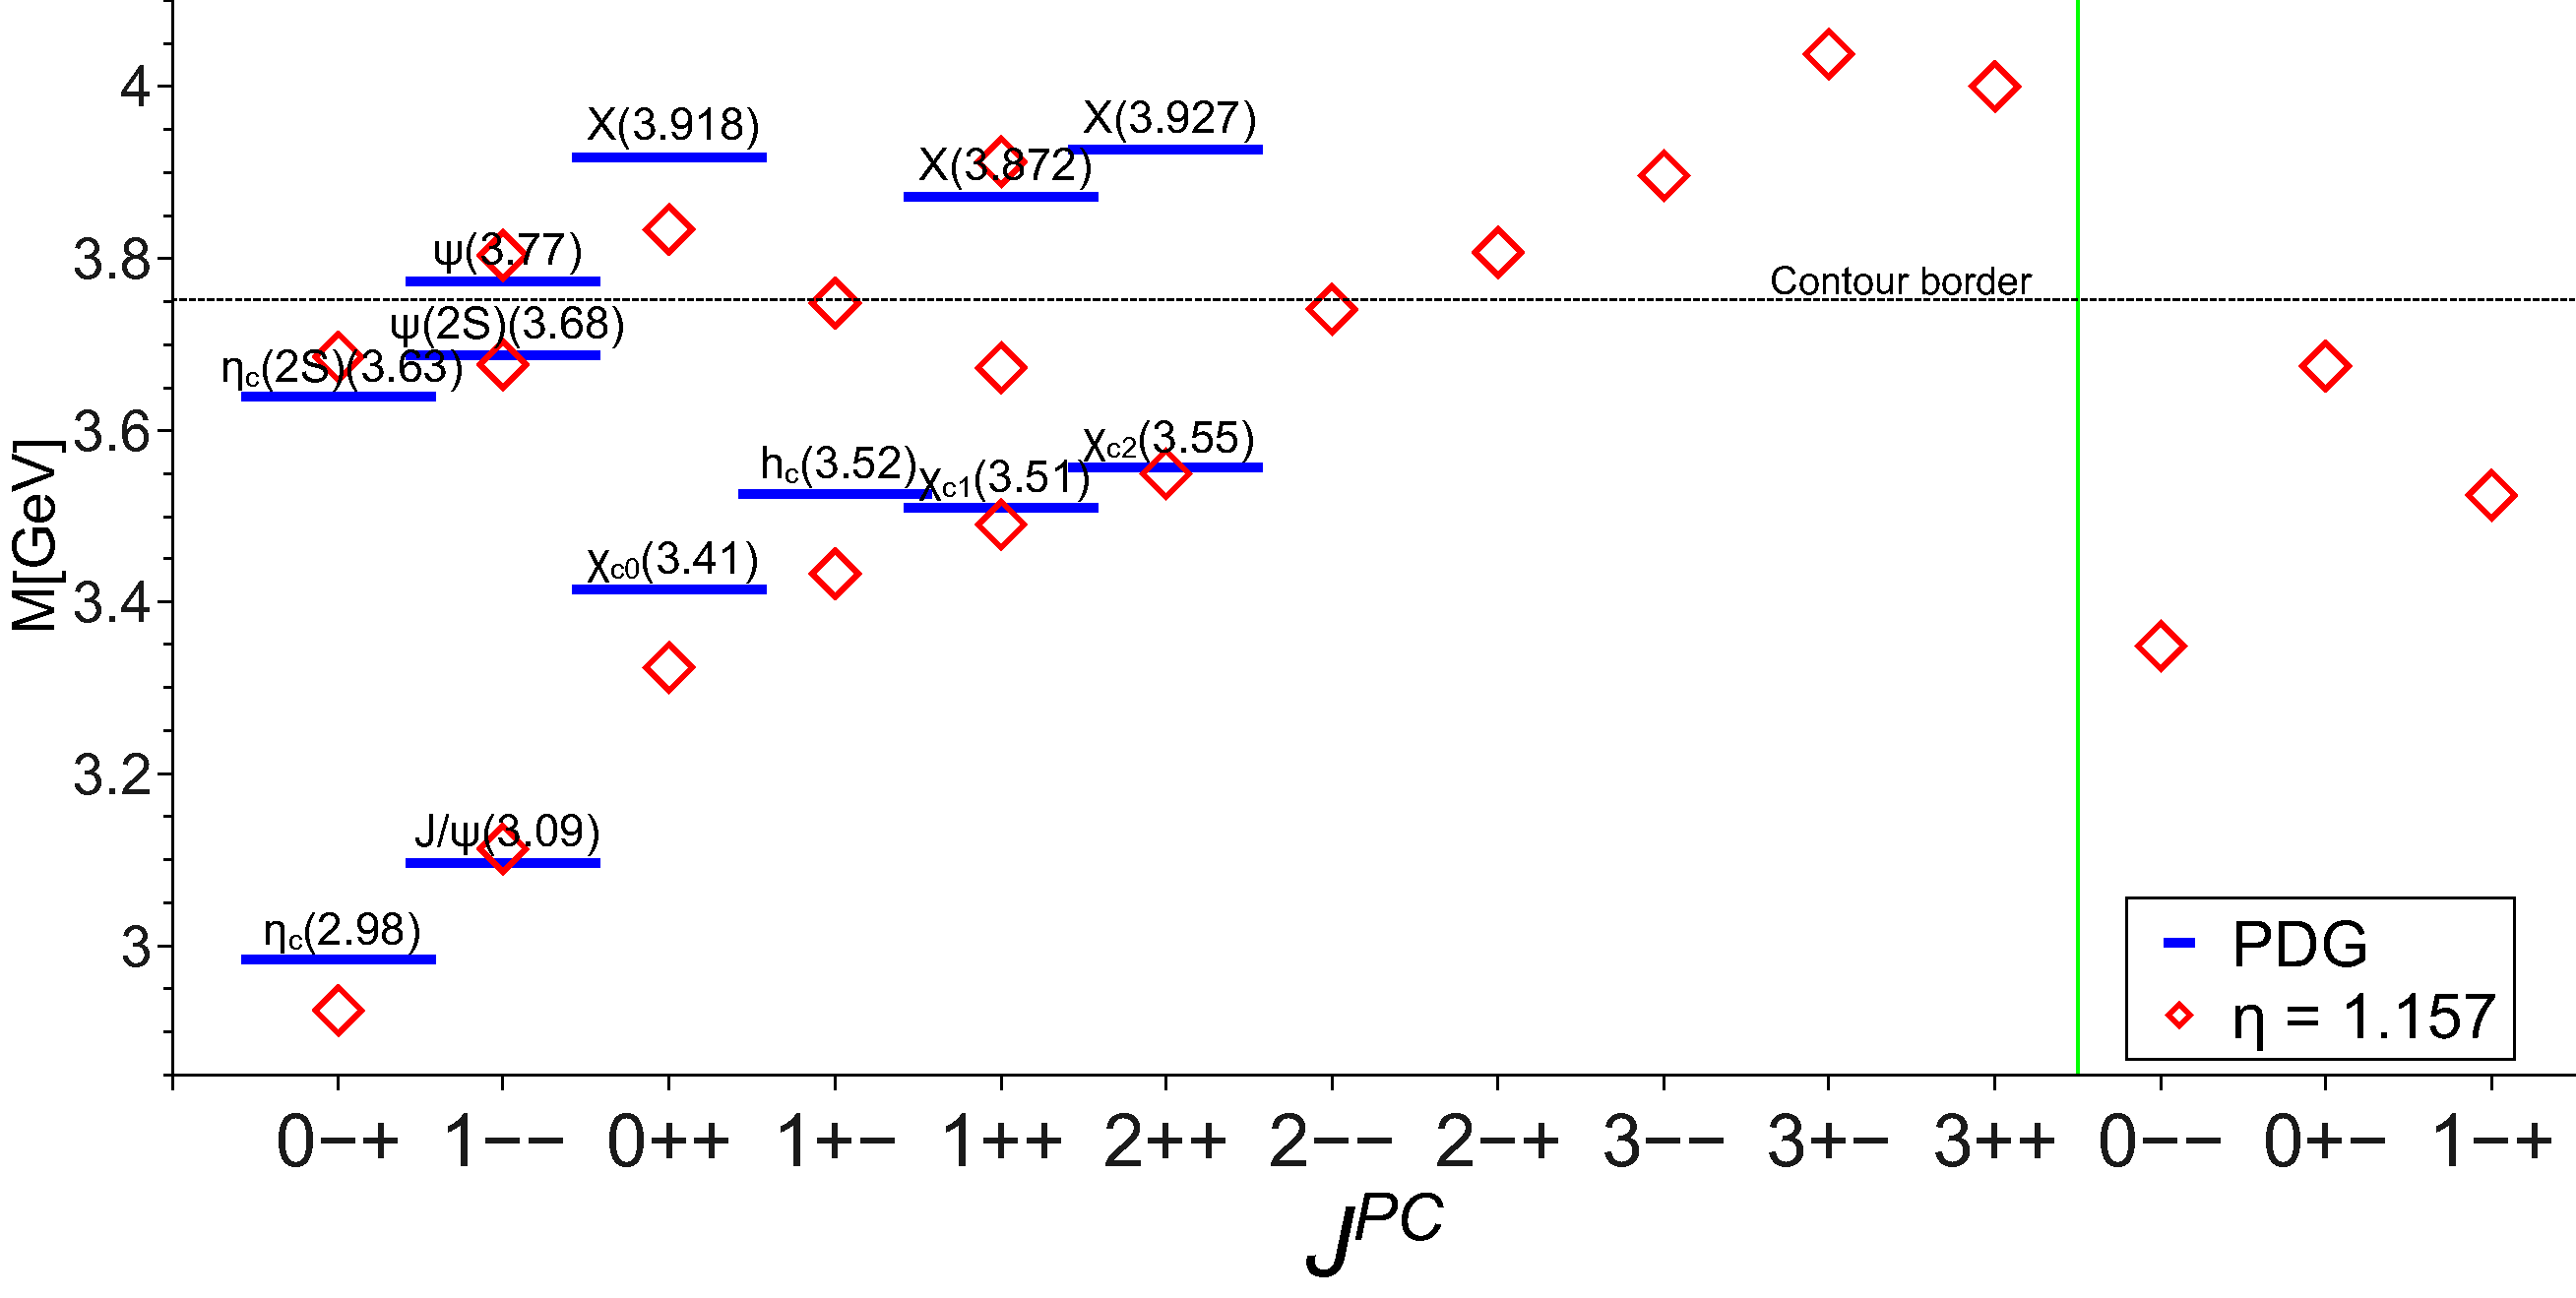
\includegraphics[width=0.999\textwidth]{figures/spectrum_cc}
  \caption{Spectrum of ground and excited charmonium states.}
  \label{fig:charm}
  \end{center}
\end{figure*}
Our results for all presently available channels are shown in Fig.~\ref{fig:charm},
the explicit values are all collected in Table. \ref{tab:results_heavy}.
Since we have fixed the two input parameters $\eta,m_{charm}$ with the $J/\Psi$ and $X_{c2}$ ground 
state, all other states can be viewed as model predictions. In the pseudoscalar channel
we find a mass of the $\eta_c$ which is slightly too low, but still within 3 \% of 
the experimental value. In the language of potential models, this may indicate an 
overestimation of the spin-spin contact term in the effective interaction. Very good 
agreement with experiment is obtained for the ground state in the $1_{++}$-channel, 
whereas the masses of the scalar $0^{++}$ and the axialvector $1^{+-}$ ground states are further 
off but still within five percent of the experimental value. Similar results have
been obtained already in Ref.~\cite{Blank:2011ha,Hilger:2014nma}. As we already observed in the light quark sector, that the rainbow-ladder interaction
is well suited to reproduce states in the sequence $1^{--}, 2^{++}, 3^{--},...$. We therefore expect our 
prediction for the mass of the $3^{--}$-state charmonium of 
%
\begin{align}
%
  m_{3^{--}}= 3.896 \,\mbox{GeV}
%
\end{align}
%
to be accurate with an error below 1~\% due to uncertainties in the interaction.
Since this state is a ground state still close to the boundary of calculable states 
(the dashed line in the plot) it is not subject to a large extrapolation error. We 
therefore expect our prediction for the mass of this state to be quite robust, with 
an overall error on the 3~\% level. Within errors, this agrees with the quark model 
prediction \cite{Ebert:2011jc} and the lattice QCD results \cite{Bali:2011rd,Liu:2012ze}.
For the other tensor ground states with $J=2$ and $J=3$ we expect much less accurate 
predictions, perhaps on the 5-10~\% level. \\ 

For the excited states we observe very good agreement in the vector channel: our
value for the mass of the $\Psi(2S)$ is very close to the experimental one, and even
the next radial excitation is nicely represented. In the pseudoscalar channel the 
splitting between the ground and the excited state is slightly too large, making the 
agreement of the $(2S)$-state with experiment even better than for the ground state
$\eta_c$. It is interesting to observe that the resulting fine structure splitting of 
the ground and excited states show a qualitatively difference when compared with 
experiment: whereas the ground state splitting is too large the splitting in the 
excited state is too low. Such an uncorrelated behaviour of the two splittings has
also been observed in lattice QCD \cite{Bali:2011rd}. \\

In the `good' tensor channel $2^{++}$ potential excited states like
the $X(3927)$ are not reproduced in our framework. There is a considerable uncertainly 
due to the extrapolation procedure needed in this mass region, which is enhanced for
excited states. Taking our result at face value, however, the current model would disregard 
the notion of the $X(3927)$ to be an ordinary meson state. \\

From an experimental point of view, the $1^{++}$-channel is perhaps the most interesting
one. There the famous $X(3872)$-state awaits its identification as a meson-molecule,
a tetraquark, or an ordinary quark-antiquark bound state. The literature on this
subject is enormous, therefore we point the reader only to Ref.~\cite{Bodwin:2013nua} 
for a first overview. The interesting question in this context is, whether a description
on a quark-antiquark basis is possible at all for the $X(3872)$. In the present
rainbow-ladder model we find an excited state in the $1^{++}$-channel at 
$m = 3672 \,\mbox{MeV}$ that cannot be accounted for by experiment. A second excitation 
is found at $m = 3912 \,\mbox{MeV}$, close to the quark model prediction for the first
excited state. In principle, it could be that the lower state of the two is spurious.
However, since we find no trace in our numerics that this is the case we disregard this
notion for the moment. It follows then, that the present form of the rainbow-ladder 
interaction is not sufficient to describe the splitting between ground and excited states
in this channel. A similar conclusion may be drawn for the other axialvector channel.
We therefore expect sizeable corrections when interactions beyond the 
rainbow-ladder approximation are taken into account. 

\subsection*{Bottomonia}\label{sec:bottom}
Our results for the spectrum of bottomonia are shown in Fig.~\ref{fig:bottom}. Compared to
the charmonium spectrum in Fig.~\ref{fig:charm} we had to change the shape of the interaction
by adjusting the $\eta$-parameter from $\eta=1.157$ for the charm-case to $\eta=1.357$ 
for the bottom quarks. This reflects part of the underlying flavour dependence of the quark-gluon 
interaction as noted in Ref.~\cite{Williams:2014iea}. Our corresponding mass of the bottom quark
is $m(19 \,\mbox{GeV})=3.790 \,\mbox{GeV}$. The resulting spectrum of ground and excited states, 
however, has similar features when compared with experimental values as the charmonium one. 
Once again, the $0^{-+}$, $1^{--}$ and $2^{++}$ ground states are well represented. The necessary
extrapolation needed for the $2^{++}$ is still under control, since the state is not too far above
the limit where everything can be calculated (the dashed line in the plot). Surprisingly good is
also the negative parity tensor state, although the extrapolation procedure in this
mass region must be considered with a little more caution. \\

Provided the good agreement in the $2^{--}$-channel can be seen as an indication that 
extrapolation even in this mass region works well, we can regard the masses of the 
further tensor states with $J=2$ and $J=3$ as solid predictions. For $3^{--}$ bottomonium bound state we found:
\begin{align}
%
  m_{3^{--}}= 10.232 \,\mbox{GeV}
%
\end{align}
Compared to the quark-model predictions of \cite{Ebert:2011jc}
we find only slight deviations of the order of 30-70 MeV for the $2^{-+}$ and the states 
with $J=3$.
%
\begin{figure*}[t]
  \begin{center}
    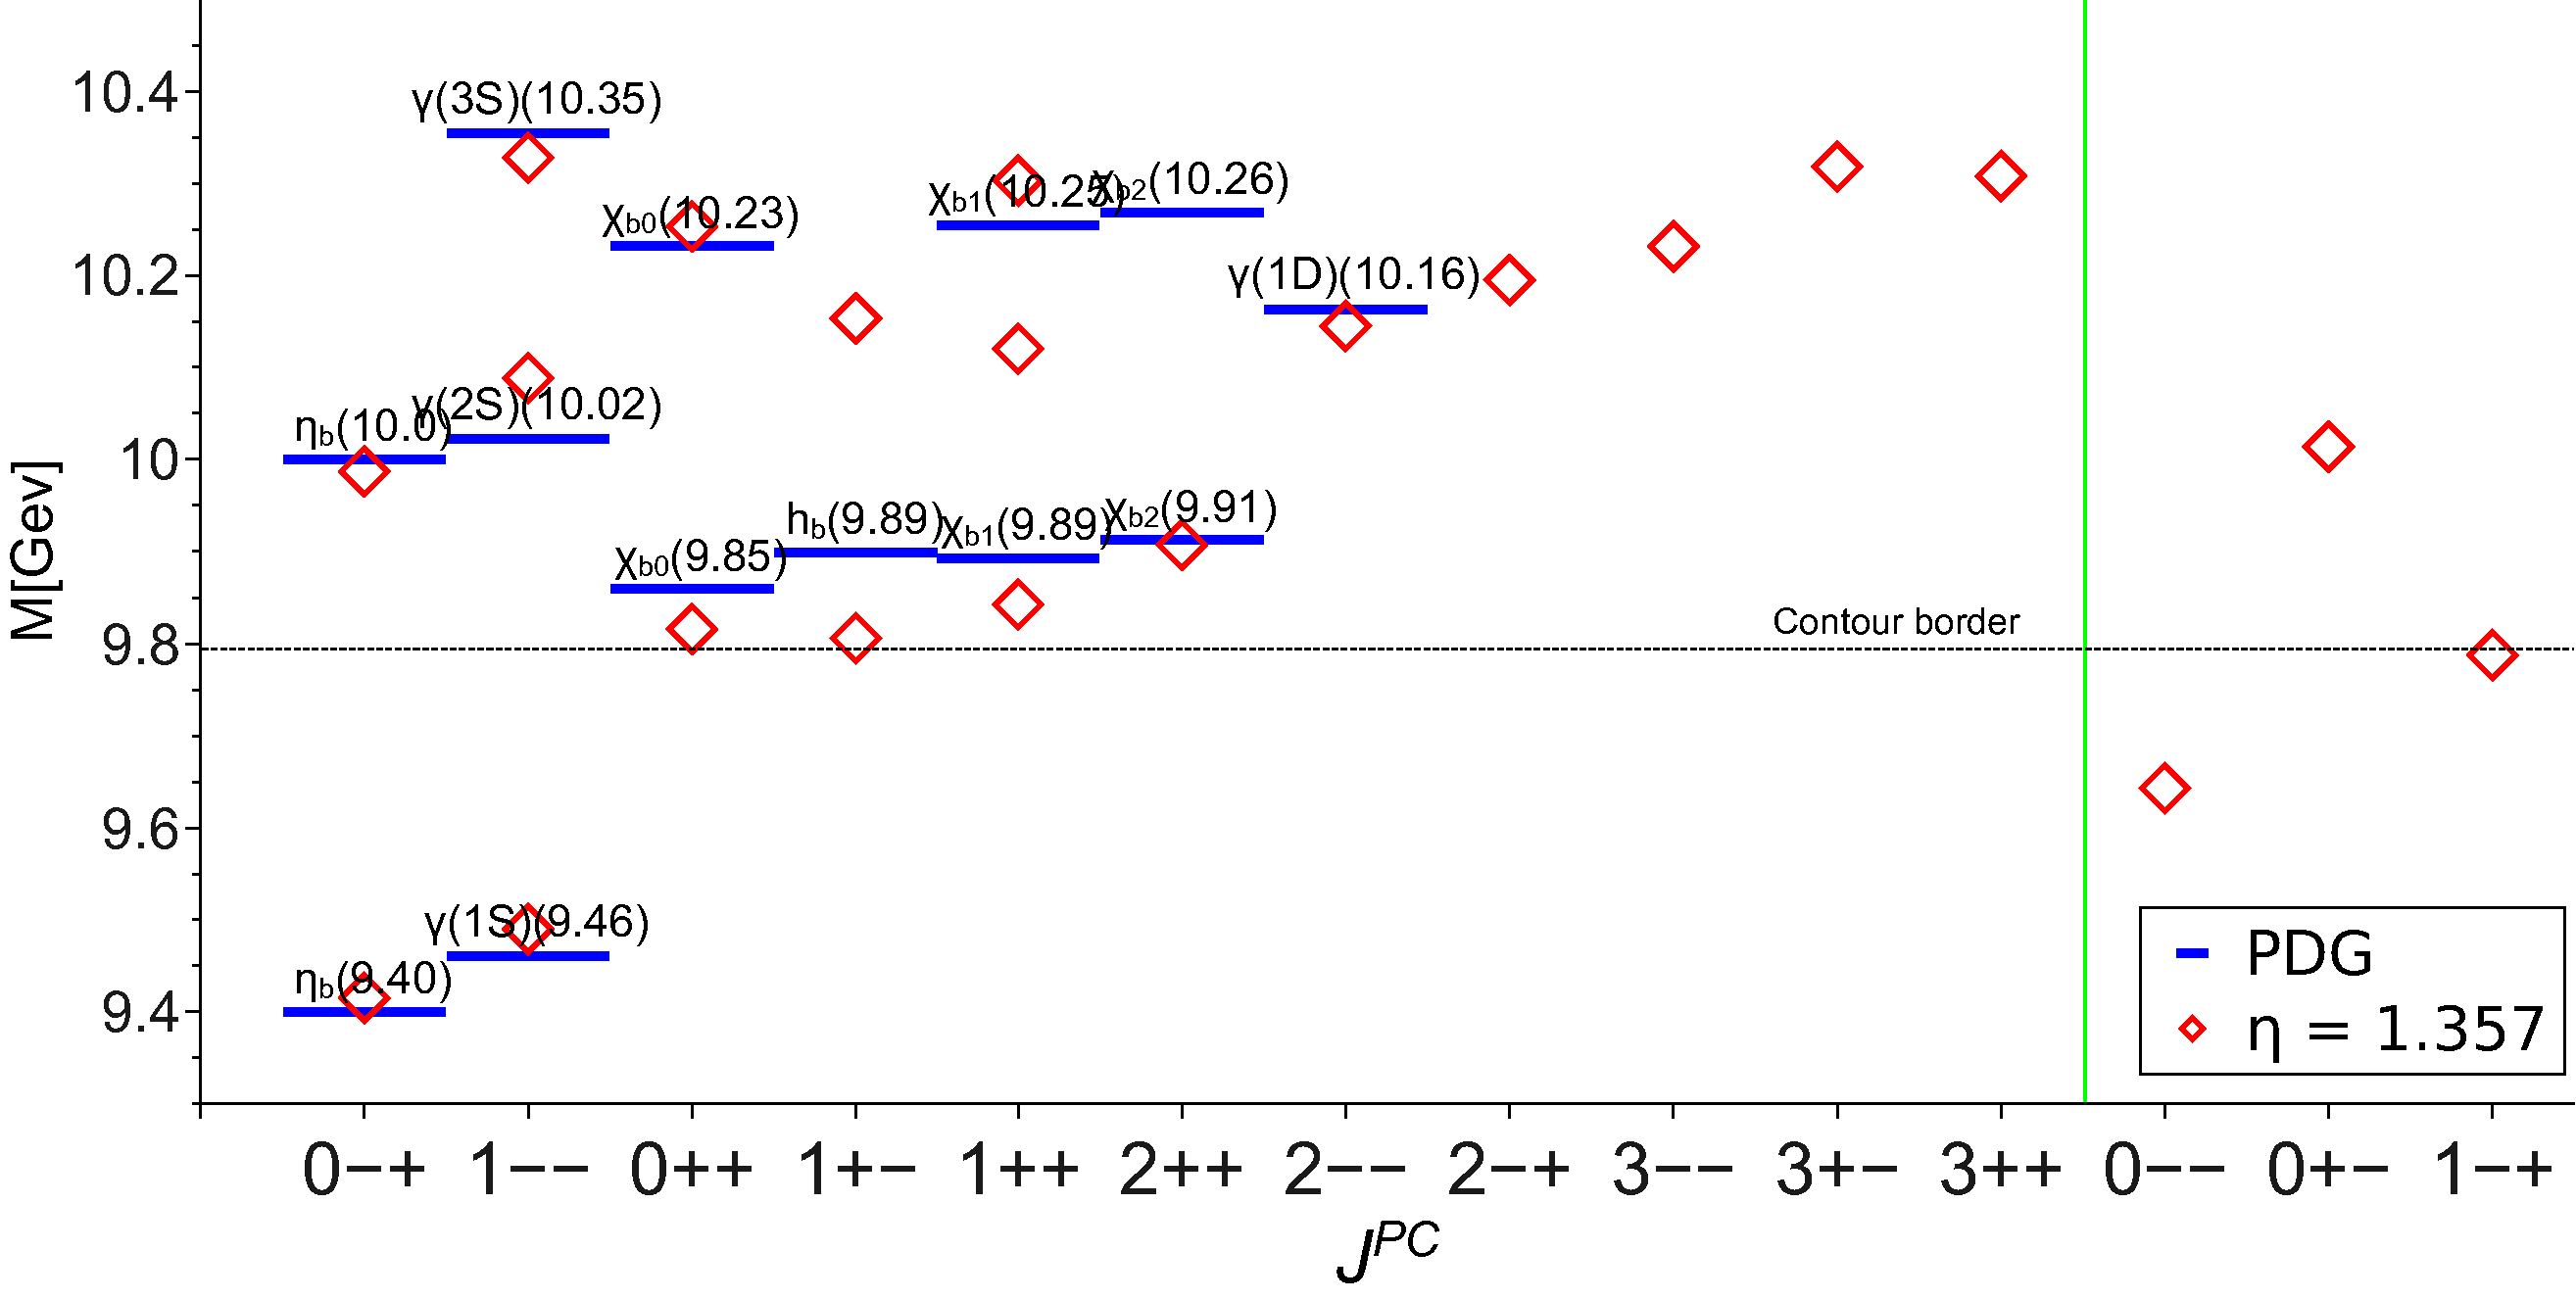
\includegraphics[width=0.999\textwidth]{figures/spectrum_bb}
    \caption{Spectrum of ground and excited bottomonium states.}\label{fig:bottom}
  \end{center}
\end{figure*}
%
In contrast to the charm-case, the lowest lying excited states in the bottomonium spectrum are
already in a mass region where we need to extrapolate the eigenvalue of the BSE, as discussed
above. Nevertheless, the results are surprisingly good and comparable with the corresponding ones in the charmonium spectrum, where much less
extrapolation was needed. The first excited states in the pseudoscalar, vector and even the
scalar channel are quite accurate and even the $\Psi(3S)$ works reasonably well. In the $1^{++}$-channel
we encounter the same problem as in the charmonium spectrum, there is a first excited state 
with a much too small mass, whereas the second excited state is not too far from a PDG-state.
%
%
%
%
%
%
\begin{figure}[!t]
  \begin{center}
    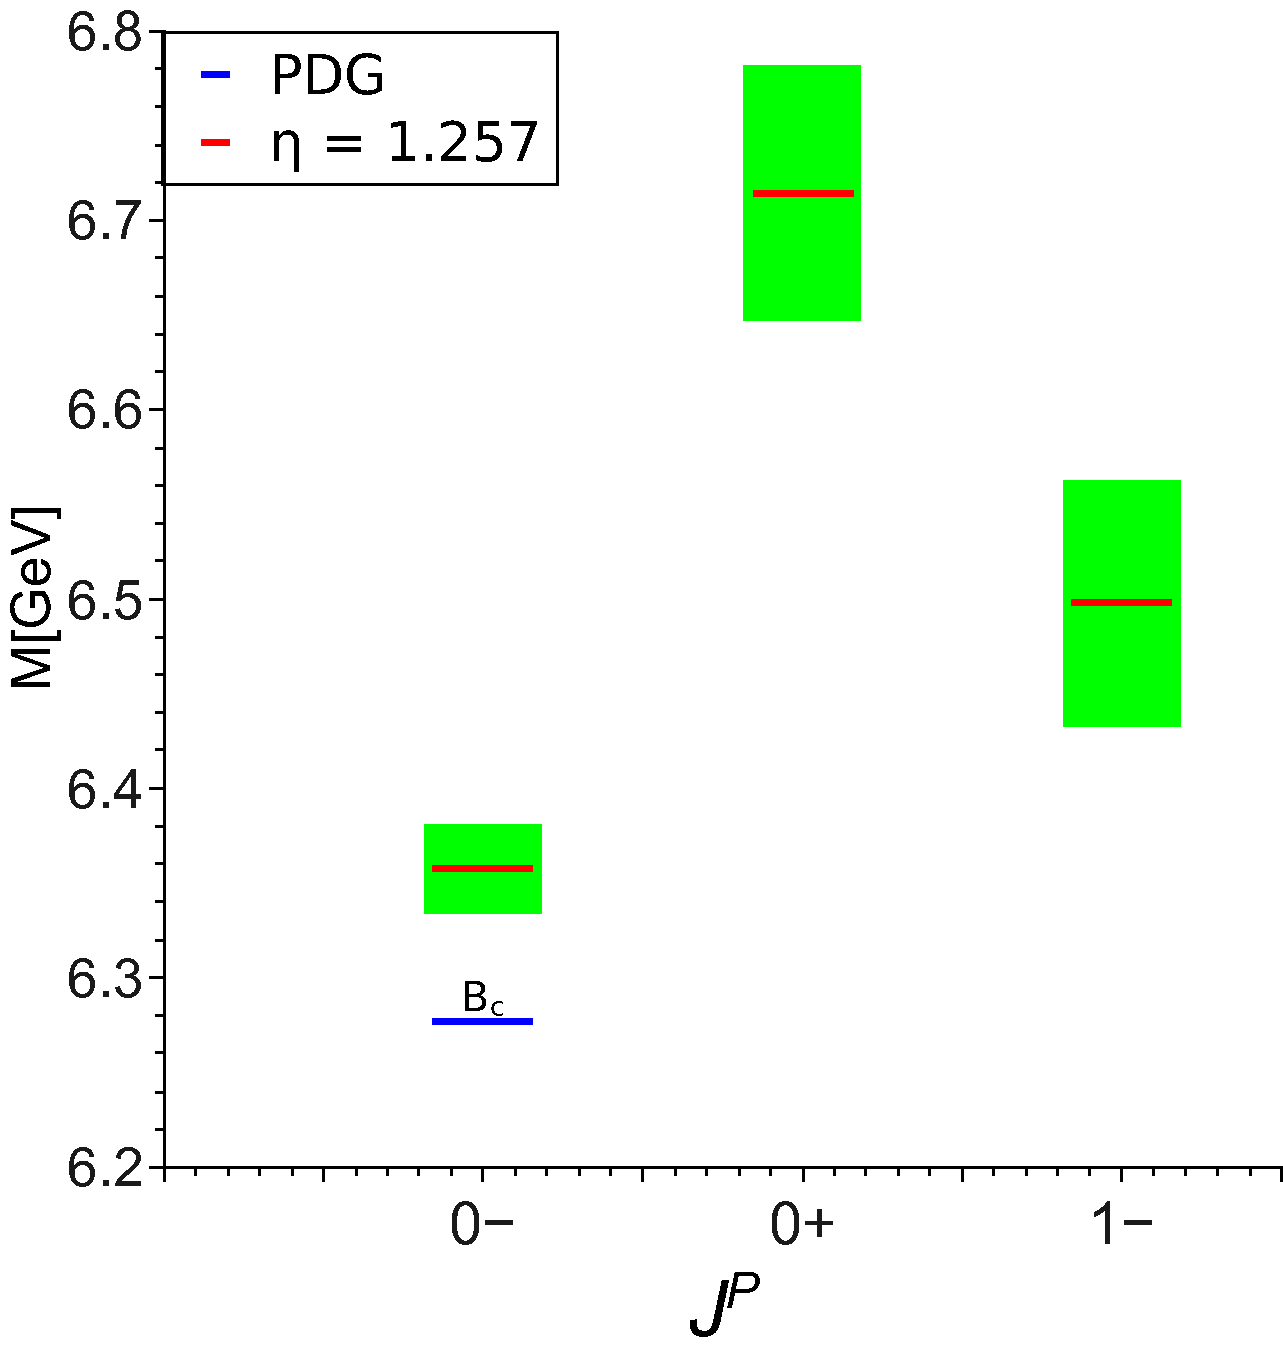
\includegraphics[width=0.45\textwidth]{figures/spectrum_bc}
    \caption{The calculated $b\bar{c}$ spectrum compared to experiment. The green bands correspond 
             to the variation $\eta=1.257\pm0.1$.}\label{fig:spectrumbc}
  \end{center}
\end{figure}
%
%
\begin{table*}[!t]
\renewcommand{\arraystretch}{1.3}
\begin{center}
\begin{tabular}{c|ccc|ccc||c|c}
\hline
\hline
            & \multicolumn{3}{c|}{$c\bar{c}   $}   & \multicolumn{3}{c||}{$b\bar{b}$}    & \multicolumn{2}{c}{$b\bar{c}$}                                         \\
$J^{PC}$    & $n=0$   & $n=1$  & $n=2$  & $n=0$   & $n=1$  & $n=2$  &  $J^{P}$ &    $n=0$                               \\
\hline                                                                                                                                                                                                     
$0^{-+}$    & $2925$  & $3684$ &        & $9414$  & $9987$ &    	&   $0^{+}$     &   $6714^{+67.1}_{-67.1}$           \\
$0^{--}$    & $3348$  &        &        & $9642$  &        &    	&   $0^{-}$   &     $6354^{+23.5}_{-23.5}$    \\
$0^{++}$    & $3323$  & $3833$ &        & $9815$  & $10254$&    	&  $1^{+}$   &                         \\
$0^{+-}$    & $3674$  &        &        & $10014$ &        &     	&  $1^{-}$  &     $6498^{+64.9}_{-64.9}$                                 \\
\hline                                                                                                                                                                                                     
$1^{-+}$    & $3524$  &        &        & $9788$  &        &    	&       &                 \\
$1^{--}$    & $3113$  & $3676$ & $3803$ & $9490$  & $10089$& $10327$&       &               \\ 
$1^{++}$    & $3489$  & $3672$ & $3912$ & $9842$  & $10120$& $10303$&       &               \\
$1^{+-}$    & $3433$  & $3747$ &        & $9806$  & $10154$&    	&       &                    \\
\hline                                                                                                                                                                                                     
$2^{-+}$    & $3806$  &        &        & $10194$  &        &    	&      &                                 \\
$2^{--}$    & $3739$  &        &        & $10145$  &        &    	&      &                                              \\
$2^{++}$    & $3550$  &        &        & $9906$   &        &    	&      &                                      \\
%$2^{+-}$   &         &        &        & $10194$  &        &    	&     &                                                                      \\
\hline                                                                                                                                                                                                     
%$3^{-+}$   &         &        &        &          &        &    	&      &                                        \\
$3^{--}$    & $3896$ &         &        & $10232$  &        &    	&      &                                           \\
$3^{++}$    & $3999$ &         &        & $10302$  &        &    	&       &                                     \\
$3^{+-}$    & $4037$ &         &        & $10319$  &        &    	&      &                                                   \\                                                                                                                                                                      
\hline
\hline
\end{tabular}
\caption{Calculated masses for ground and excited charmonium, bottomonium and charm-bottom states.}\label{tab:results_heavy}
\end{center}
\end{table*} \\

Finally, we present our results for selected channels of $B_c$-mesons. 
Heavy-light systems in the Bethe-Salpeter% PARTITIONING OPTIMIZATION \beware 
approach are notoriously difficult to treat, since the problem of probing the analytical
structure of the internal quark propagators already appears for ground states, see e.g.
Ref.~\cite{Rojas:2014aka,Gomez-Rocha:2014vsa} for recent studies of the problem. Our results for these states,
shown in Fig.~\ref{fig:spectrumbc} are therefore all extrapolated and have a systematic error
of about 5-10 \%. In the plot we show values obtained using a variation of the $\eta$-parameter
in the interaction ranging approximately between the ones used for the charmonia and bottomonia.
In this way we heuristically take into account the varying strength of the interaction for the
two different quark flavours involved. The central value, given by the red line, corresponds 
to $\eta=1.257$. Given the inherent uncertainties in the calculation, our value for the $B_c$
in the pseudoscalar channel is surprisingly close to the experimental one. Since this is the
state with the lowest mass, the extrapolation error is also smallest. Since the rainbow-ladder
approach works well in the vector channel we consider the existence and to some extent also the 
mass of the vector state as a prediction of the approach, whereas the scalar channel has to
be considered with much more reservation. Despite these sources for errors it is interesting to
note that our results for all three states agree qualitatively with the ones in the relativistic 
quark model of Ref.~\cite{Ebert:2011jc} with quantitative deviations of at most 3~\%.

\subsection*{Effective interaction variation}\label{int1}
As we saw, the interaction between heavy quarks, represented by effective singe gluon exchange, leads to 
the spectrum coinciding with experimental values with in 5\%. The main reason for that is the huge set of diagrams like: hadronic exchange, quark loops and etc. are suppressed by heavy quark mass. From this fact follows that the charmonium meson bound state is a prefect test-ground for a effective gluon models. Therefore it is interesting to explore the response of the mass spectrum to the variation of the shape of the effective gluon coupling $\alpha_{eff}$. In order to proceed with this idea we would like to replace the original Maris and Tandy model \cite{Maris:1999nt}, which explicit expression is:
\beqa
\label{spec:MT_model}
\alpha_{\mathrm{eff}}(q^2)=\pi\eta^7x^2e^{-\eta^2x}
+\frac{2\pi\gamma_m\left(1-e^{-y}\right)}{\log\left[e^2-1+(1+z)^2\right]}\;,
\eeqa
with more generalized form:
\begin{align}\label{spec:generalmaristandy}
%
  \alpha_{\mathrm{eff}}(q^2)=\alpha_{\mathrm{IR}}(q^2)+\alpha_{\mathrm{UV}}(q^2)\;,
%
\end{align}
%
where
%
\begin{align}\label{spec:generalmaristandy2}
%
  \alpha_{\mathrm{IR}}(q^2) &= \pi\eta^7\mathcal{P}(x)e^{-\eta^2x}\;,\\
  \alpha_{\mathrm{UV}}(q^2) &= \frac{2\pi\gamma_m\left(1-e^{-y}\right)}{\ln\left[e^2-1+(1+z)^2\right]}\;.
%
\end{align}
Since expect the shape of the interaction to change we therefore employ the polynomial form for $\mathcal{P}(x)$:
\begin{align}\label{spec:polinomMT}
%
  \mathcal{P}(x) = \sum_{i=1}^n a_i x^{i}\;.
%
\end{align}
%
and investigate its impact on the heavy meson spectrum restricting ourselves 
to terms with $n \le 4$. Note that $a_2=1$ and other $a_n=0$ corresponds to original Maris and Tandy model. 
\begin{figure}[!t]
  \begin{center}
    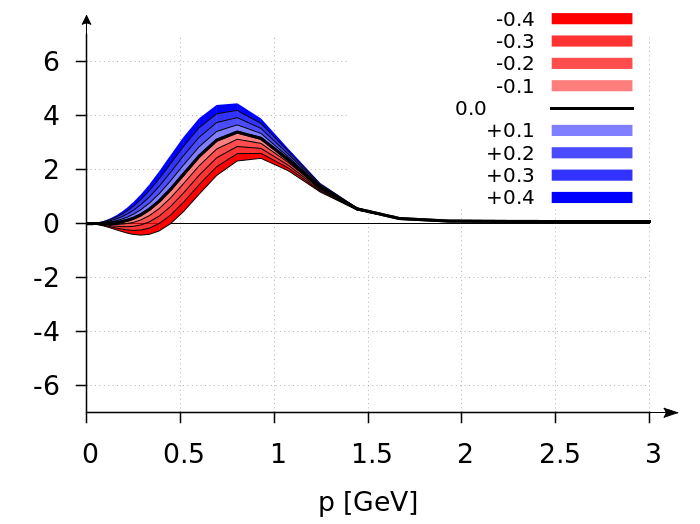
\includegraphics[width=0.49\textwidth]{figures/maris_a1}
    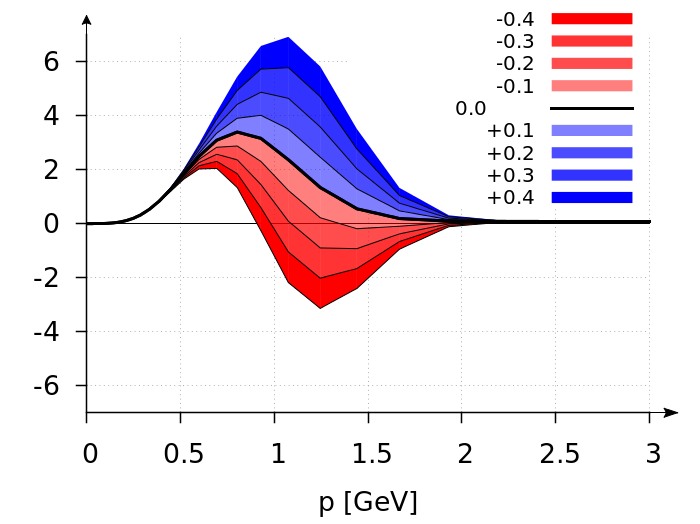
\includegraphics[width=0.49\textwidth]{figures/maris_a4}
    \caption{The shape of the effective coupling for the generalized Maris-Tandy interaction with $a_2=1$ held constant
             and varying $a_1$ and $a_4$. Left graph corresponds to the variation of $a_1$ and right one to the variation of $a_4$. }
    \label{fig:slope_a1}
  \end{center}
 \end{figure} \\
 
First we vary $a_1$ in the interval
$-0.5 \le a_1 \le 0.5$. For the effective running coupling the resulting variation
is shown in Fig.~(\ref{fig:slope_a1}). Clearly, the integrated strength, but
also the fine details of the coupling change: For negative $a_1$ we even obtain 
a zero crossing with the corresponding scale associated with the relative
strength between the $a_1$ and $a_2$-terms (here we keep $a_2=1$). Such an 
effective coupling is unusual, but not unreasonable. Recent calculations of 
the three-gluon vertex \cite{Aguilar:2013vaa,Blum:2014gna,Eichmann:2014xya} suggest that the interplay between 
ghost and gluon degrees of freedom in the corresponding Dyson-Schwinger equation 
for the vertex may very well introduce such a zero crossing. This possibility is also 
seen in corresponding lattice calculations \cite{Cucchieri:2008qm}. Since the three-gluon 
vertex is an integral part of the non-Abelian diagrams in the DSE for the quark-gluon vertex, 
this behaviour may translate into a corresponding zero crossing of the quark-gluon 
vertex~\cite{Williams:2014iea} and subsequently into the effective coupling.  
 \begin{figure}[!t]
  \begin{center}
    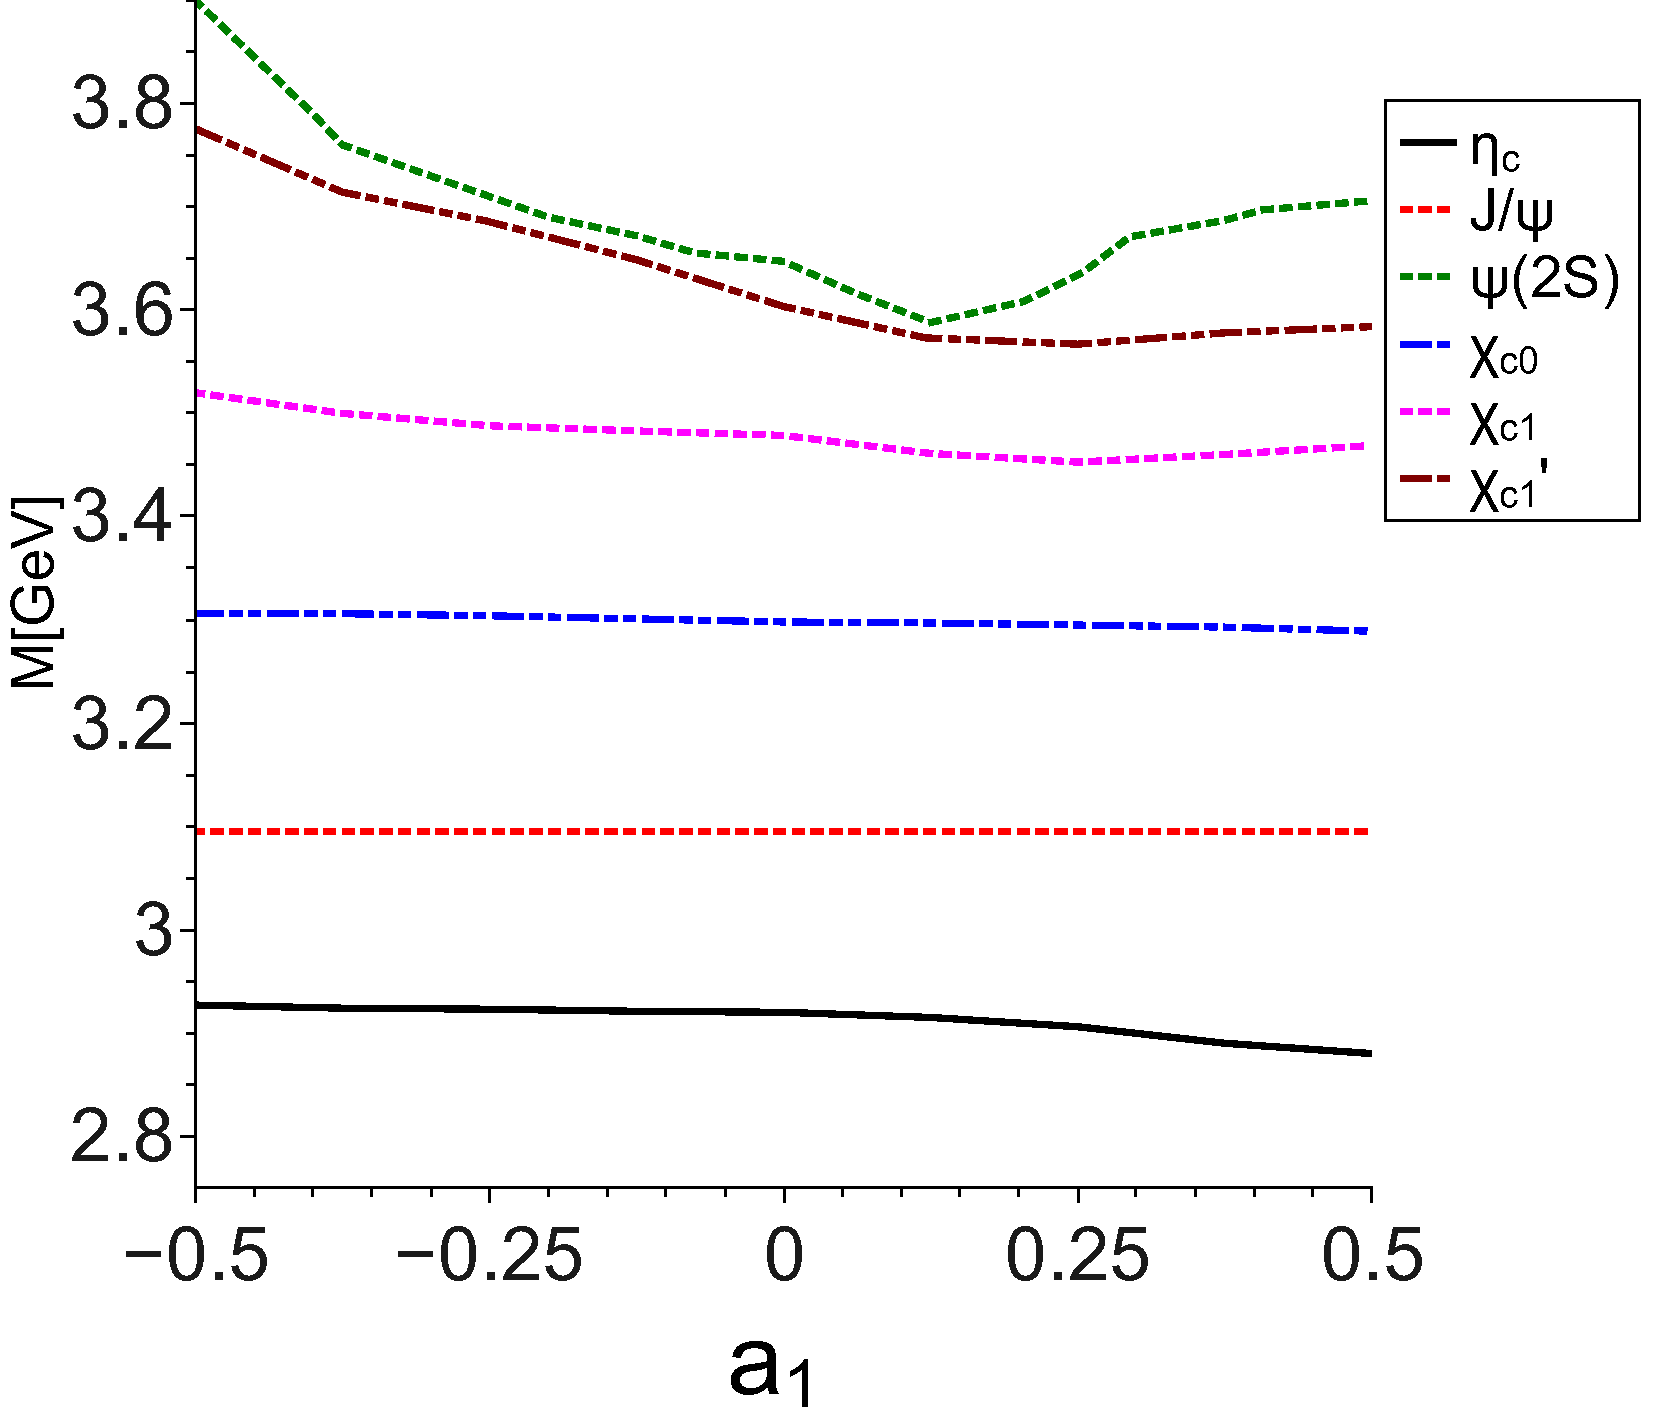
\includegraphics[width=0.49\textwidth]{figures/trend_a1_CC}
    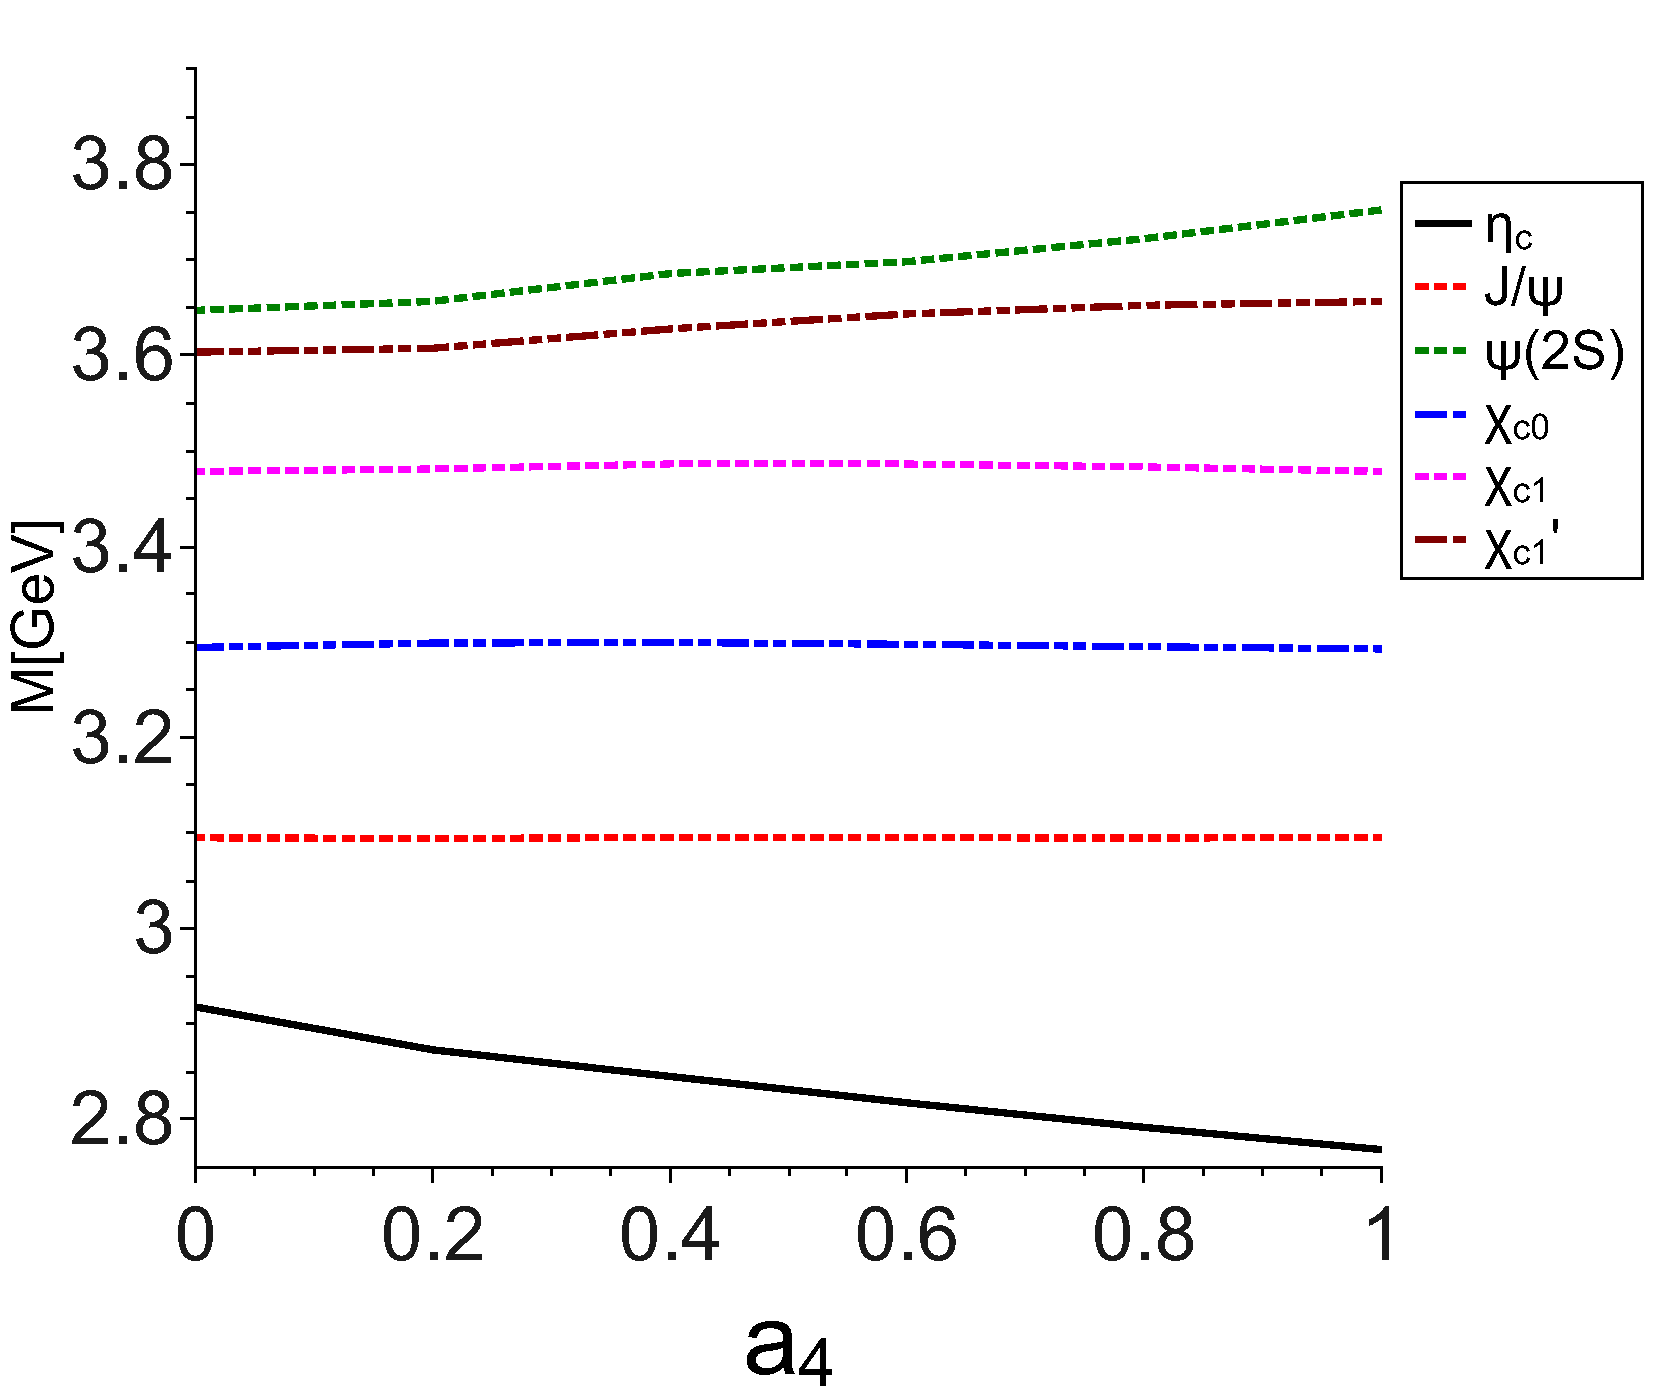
\includegraphics[width=0.49\textwidth]{figures/trend_a4_CC} 
    \caption{The response of masses of bound and excited states on the variation of the shape 
             of the effective interaction with $a_1$ and $a_4$ correspondingly.}
    \label{fig:trend_a1}
  \end{center}
\end{figure} \\

The resulting changes in the meson spectrum are displayed in 
Fig.~\ref{fig:trend_a1}. Adjusting the bare charmonium quark mass via $m_{J/\Psi}$
to accommodate for the changes in the integrated interaction strength we
observe only very small changes in the resulting masses for the ground state mesons.
However, the excited states $\Psi(2S)$ and $\chi_{c1}^{\prime}$ turn out to be very sensitive 
to the details of the interaction. In particular for negative values of $a_1$,
corresponding to the zero crossing of the interaction discussed above, we find much
increased values for the mass of the $\chi_{c1}^{\prime}$, which eventually even may 
hit the experimentally observed mass of the $X(3872)$. However, this comes at a price: 
the mass of the $\Psi(2S)$ reacts in a similar way and substantially moves away from 
the experimental value, almost reproduced for $a_1=0$. We therefore conclude, that 
by changing the infrared behaviour of our rainbow-ladder interaction it is not possible 
to accommodate for the quark-antiquark nature of the $X(3872)$, while at the same time 
keeping the remaining spectrum intact. \\

Next we consider the generalized Maris-Tandy interaction, Eq.~(\ref{spec:generalmaristandy2}), 
given by $a_1=0$, $a_2=1$ but non-trivial components $a_3$ or $a_4$. Both of these modify 
the interaction in the intermediate momentum region, while keeping the infrared and
ultraviolet behaviour untouched as can be seen from Fig.~\ref{fig:slope_a1} for the 
example of variations in $a_4$. Since variations of $a_3$ act similarly on the effective
coupling we keep $a_3=0$ fixed and restrict ourselves to variations of $a_4$.
Furthermore, we keep $a_4 \ge 0$, since there are no indications that the dressing of the
quark-gluon vertex can induce a negative effective interaction in the mid-momentum region. \\

Again, we study the variation of the charmonium spectrum while still readjusting
the charm quark mass to reproduce the vector ground state $J/\Psi$. Our results
are given in Fig.~\ref{fig:trend_a1}. Here we find a substantial increase in the
mass splitting between the pseudoscalar and the vector channel due to the additional
interaction strength in the mid-momentum region. At the same time, the masses of the
excited state, $\Psi(2S)$ and $\chi_{c1}^{\prime}$ increase slightly. This moderate increase 
is nowhere large enough to bring the $\chi_{c1}^{\prime}$ close to the observed $X(3872)$-state.
Thus we arrive at the conclusion that by changing the mid-momentum behaviour of our 
interaction it is not possible to accommodate for a quark-antiquark nature of the 
$X(3872)$, while at the same time keeping the remaining spectrum intact.
%
%
%
%

\section{Regge trajectories}\label{res:regge}
Finally, we present results for Regge trajectories in Fig.~\ref{fig:regge} for natural parity states. 
At first, we consider the ground states of the light quark meson spectra; for the corresponding excited states and the 
other channels we do not have enough bound states with $J=2,3$ to probe for trajectories. 
One immediately notes that, indeed, the sequence $J^{PC}=1^{--}, 2^{++}, 3^{--}$ forms an almost linear
trajectory in the $(M^2,J)$-plane. This is interesting, since we are working with a model that is
apparently \emph{not} related to a linear rising potential between light quarks. 
\begin{figure}[h]
\begin{center}
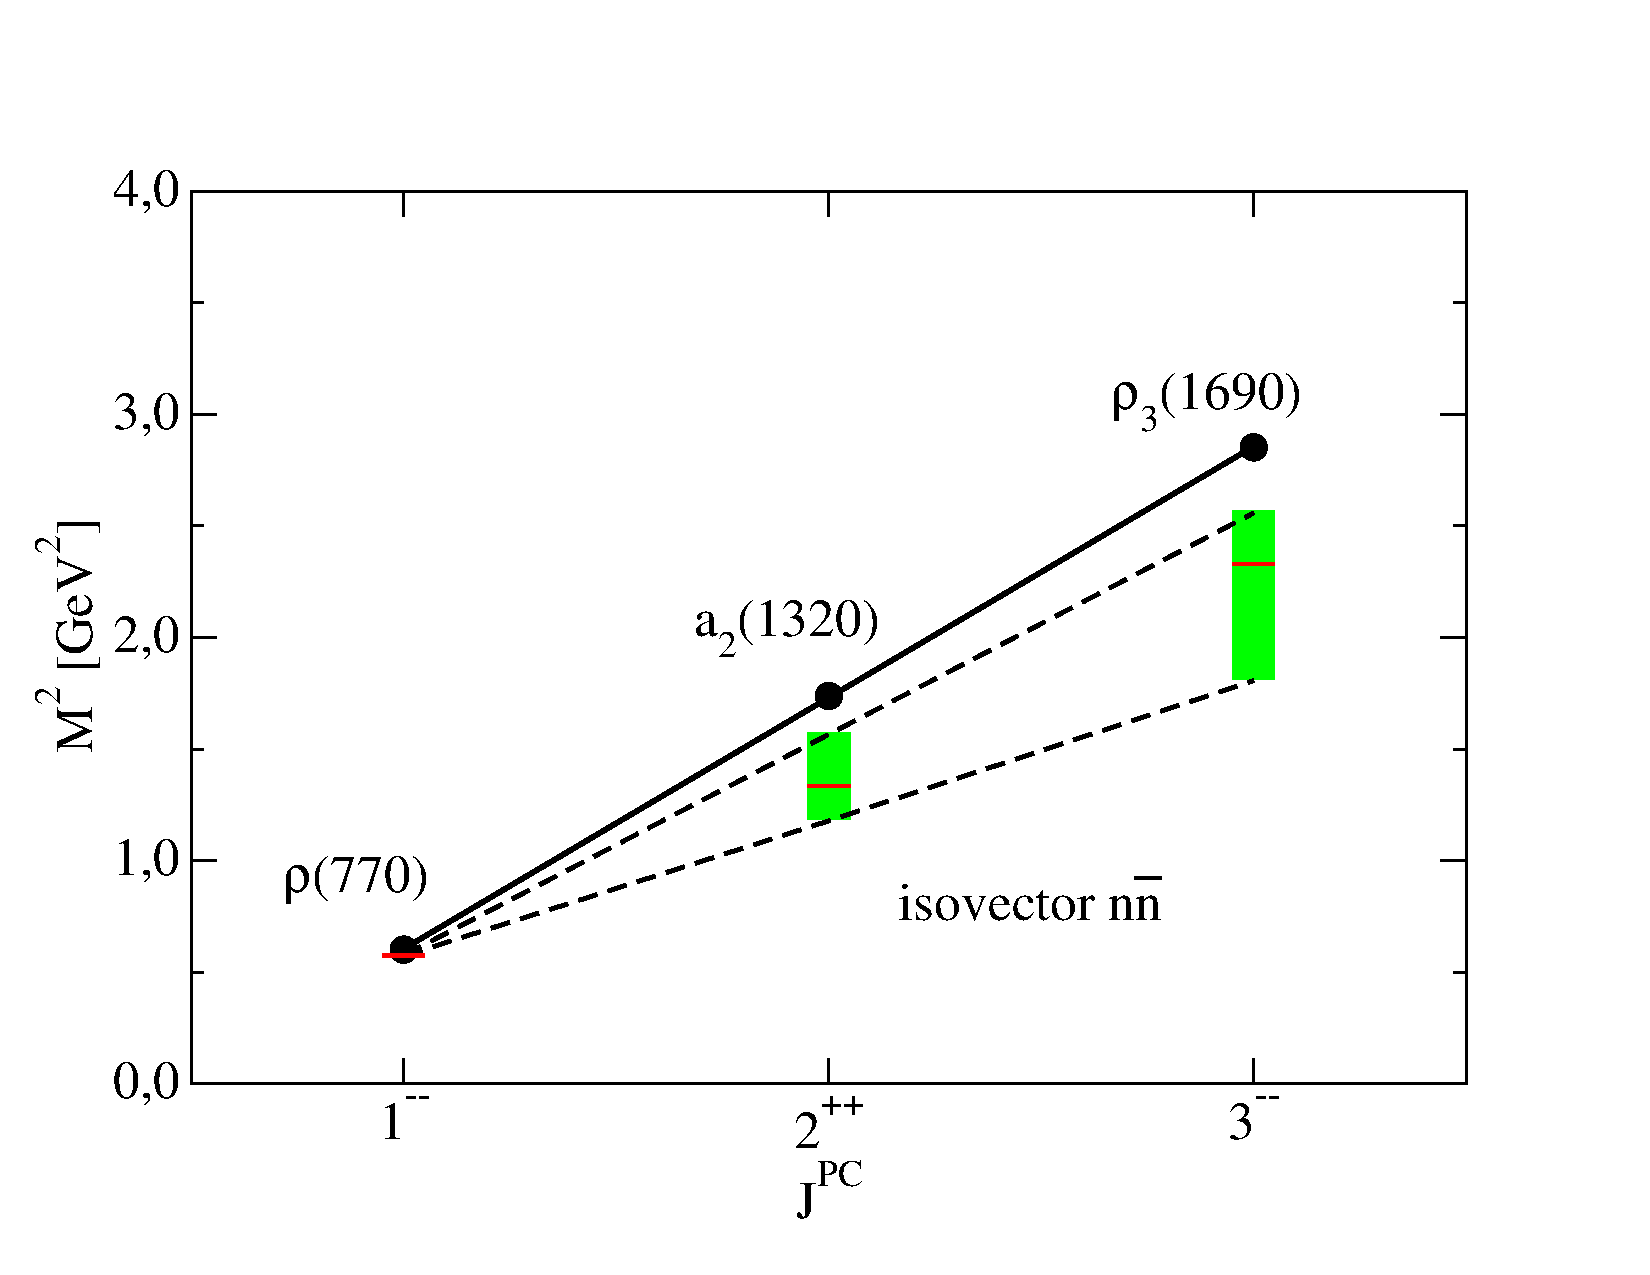
\includegraphics[width=0.49\textwidth]{figures/reggenn_v2}
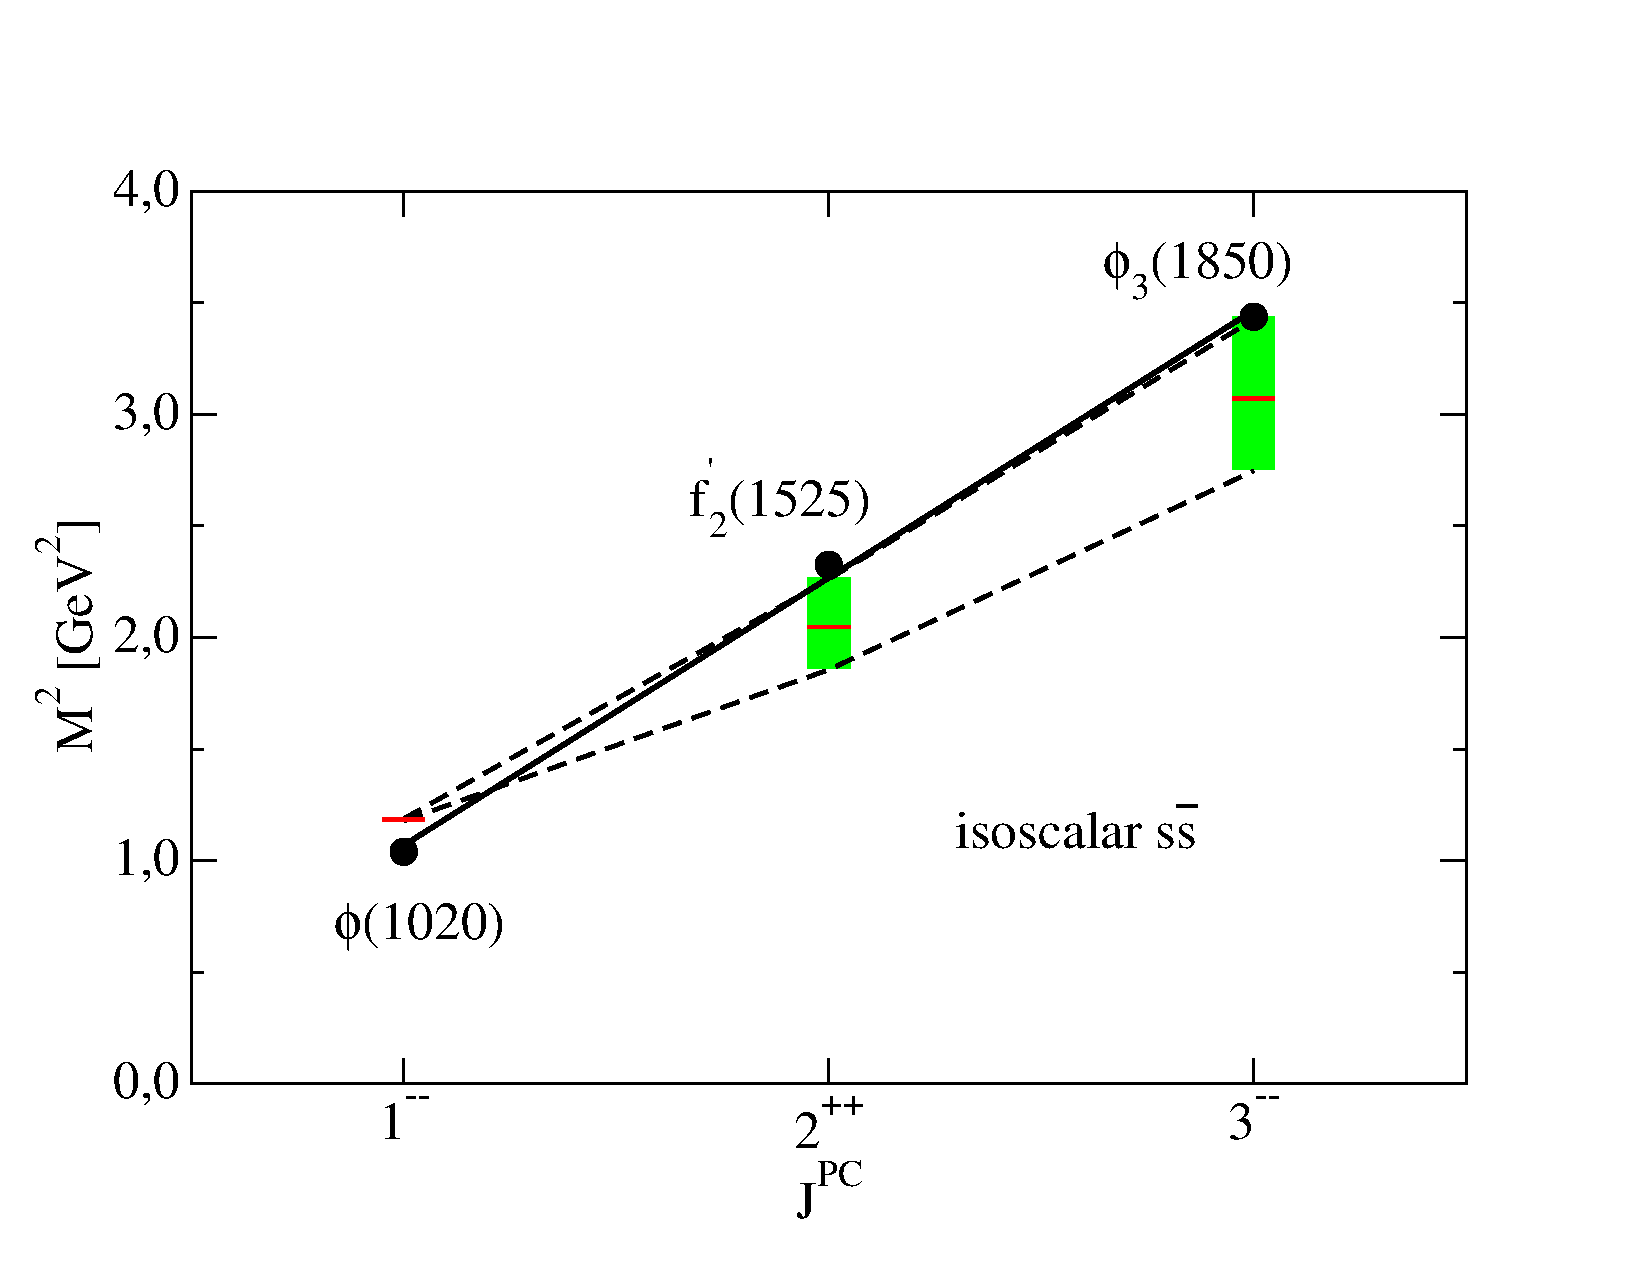
\includegraphics[width=0.49\textwidth]{figures/reggess_v2}
\caption{\small Regge trajectories for isovector $n\bar{n}$ (upper plot)
and isoscalar $s\bar{s}$ mesons (lower plot) with natural parity. 
Filled circles correspond to experimental data, while calculated values are given by the red marks
for $\eta = 1.8$ and the green bands for $\eta = 1.8 \pm 0.2$. The resulting Regge trajectories for 
the upper and lower end of the bands are displayed by the dashed lines. Not shown is the numerical
error of our mass extraction procedure, which is of the order of 5-10 $\%$ for the $J=2,3$ states.}\label{fig:regge}
\end{center}
\end{figure} 
Thus, the conventional, naive but intuitive explanation for the formation of Regge-trajectories does not apply
in our framework. Nevertheless, we see an (approximate) $\rho$- and $\phi$-meson Regge trajectory 
for our results. The slope of the trajectory is easily extracted. With
\begin{equation}
M^2_X(J) = M^2_X(0) + \beta_X J
\end{equation} 
we find
\beqa
M^2_\rho(0)& = -0.42 \,\,(-0.05)\,\, \mbox{GeV}^2 \;\;\;\;  M^2_\phi(0)& = \,\,0.05 \,\,(0.36)\,\, \mbox{GeV}^2 \nonumber\\
\beta_\rho & = \,\,0.99 \,\,(0.62)\,\, \mbox{GeV}^2  \;\;\;\;\;\;\;\;\;\;\;\;\;\;\; \beta_\phi &  = \,\,1.12 \,\,(0.78)\,\, \mbox{GeV}^2 \nonumber
\eeqa
for $\rho$ and $\phi$ respectively. The two numbers each correspond to the upper (lower)
end of the $\eta$-band of our results. Compared to recent studies of Regge trajectories
based on the $\rho$-meson, $\beta_\rho = 1.19 \pm 0.10$ GeV$^2$ \cite{Masjuan:2012gc} and 
$\beta_\rho = 1.11 \pm 0.01$ GeV$^2$ \cite{Londergan:2013dza}, our number for the slope at the
upper edge of the $\eta$-band is smaller by only about 
ten percent. Recalling that we need to employ an extrapolation procedure in the complex 
momentum plane to extract the bound state mass of the tensor states with an error margin 
of the order of 5-10 $\%$ the agreement is quite good.
We have also checked for Regge trajectories in channels with unnatural parity and found an 
approximate linear trajectory also for the sequence $J^{PC}=1^{++}, 2^{--}, 3^{++}$ based 
on the $a_0$. Again, for the other channels and the excited states we find not enough bound 
states with $J=2,3$. From the discussion in the previous sections we furthermore expect, 
that the slopes and intercepts in these channels may be further off the experimentally extracted 
values, simply because the rainbow-ladder interaction is not good enough in these channels. 
Indeed for the $a_0$-trajectory we find $M^2_{a_0}(0) = 0.20\,\, \mbox{GeV}^2$ and
$\beta_{a_0} = 0.78 \,\,\mbox{GeV}^2$ for the upper edge of the $\eta$-band, which do not 
agree too well with {\it e.g.} the values found in Ref.~\cite{Ebert:2009ub}, 
$M^2_{a_0}(0) = -0.658 \pm 0.120\,\, \mbox{GeV}^2$ and
$\beta_{a_0} = 1.014 \pm 0.036 \,\,\mbox{GeV}^2$. \\

As for the heavy quark systems, similar to the light quark sector we also find, that the 
sequence $1^{--}, 2^{++}, 3^{--}$ lies on a Regge-trajectory with an accuracy that is
even better than in the potential model of Ref.~\cite{Ebert:2011jc}. 
For $M^2_X(J) = M^2_X(0) + \beta_X J$ we find $M^2_{J/\psi}(0) = 2.72$ and $\beta_{J/\psi} = 0.39$ for charmonium natural parity states and
for bottomonium - $M^2_{\Upsilon}(0) = 9.12$ and $\beta_{\Upsilon} = 0.371$, which 
is also somewhat steeper than the result of \cite{Ebert:2011jc}. For the heavy quark 
sector this confirms a result for light quarks, that Regge-type behaviour in the spectrum may be 
found without any direct connection to an underlying string-picture.
%
%
%
%
%
%In this work we presented a first calculation of ground and excited states with angular 
%momentum $J \le 3$ in the heavy quark sector using the framework of Dyson-Schwinger 
%and Bethe-Salpeter equations. We have used a simple interaction model, the rainbow-ladder
%approximation, which is known to represent only part of the complicated interaction
%pattern of quarks and gluons even for heavy quarks. Nevertheless, we obtained surprisingly 
%good results, at least for selected quantum numbers. In general, the systematics in the 
%spectrum for charmonia and bottomonia is very similar, although the underlying interaction 
%is not the same. Compared to the light quark sector, where
%the rainbow-ladder approximation has clear deficiencies \cite{Fischer:2014xha}, the agreement with
%the experimental states is much improved. This is particularly true for the ground and 
%excited charmonia and bottomonia states in the vector channel, where even the second 
%radial excitation is well represented. For pseudoscalar states and tensor states with quantum 
%number $2^{++}$ we obtain reasonable results, whereas for scalars and axialvectors some
%deviations occur. We also gave predictions for the other tensor states, in particular
%for the $3^{--}$, which should be a channel where the rainbow-ladder approximation
%does particularly well. For the bottomonia, our values for the tensor states may be 
%considered as solid predictions for experiment with a systematic error due to 
%extrapolations on the 1~\% level. We also gave results for $B_c$ states and quarkonia 
%with exotic quantum numbers, although the accumulated errors in these channels due to
%deficiencies in the rainbow-ladder interaction may be sizeable.
%
%Furthermore, we studied variations of the shape of the rainbow-ladder effective coupling with 
%the aim to explore whether the first excitation in the $1^{++}$-channel can be linked 
%to the $X(3872)$ without destroying other parts of the spectrum. It turned out, that 
%this is not possible. Thus either hitherto not included corrections beyond rainbow-ladder
%play an important role in this channel, or the $X(3872)$ does indeed not have a strong
%quark-antiquark component. From the perspective of our framework, these questions remain 
%open until studies beyond rainbow-ladder are available. 
%
%Clearly, the findings of this work should be corroborated by studies beyond the 
%simple rainbow-ladder scheme used in this work. Within the light meson sector
%several approaches in this direction have been explored in the past 
%\cite{Watson:2004kd,Fischer:2005en,Fischer:2008wy,Fischer:2009jm,Chang:2009zb,Heupel:2014ina}
%and it remains to be seen whether these can be transferred to the heavy quark 
%sector. This will the subject of future work.
	



\chapter{Pion Cloud Effect}
\label{chap:pion}
There are, however, also severe limitations to the 
rainbow-ladder scheme. Consequently, much work has been 
invested in the past years on its extension towards more 
advanced approximations of the quark-gluon interaction. 
On the one hand, this may be accomplished directly by devising
improved \textit{ans\"atze} for the dressing functions of the 
quark-gluon vertex 
\cite{Fischer:2005en,Chang:2009zb,Chang:2010hb,Heupel:2014ina}.
On the other hand, it is promising to work with diagrammatic
approximations to the vertex DSE. While most studies so far concentrated 
on ($1/N_c$-subleading) Abelian contributions to the vertex (see e.g. 
\cite{Bender:1996bb,Watson:2004kd,Watson:2004jq,Bhagwat:2004hn,Matevosyan:2006bk}),
the impact of the $1/N_c$-leading, non-Abelian diagram on light meson
masses has been investigated in \cite{Fischer:2009jm}. In addition,
important unquenching effects in the quark-gluon interaction may 
be approximated by the inclusion of hadronic degrees 
of freedom \cite{Fischer:2007ze,Fischer:2008sp,Fischer:2008wy}. 
This is possible, since the vertex DSE can be decomposed on a diagrammatic
level into terms that are already present in the quenched theory and those 
involving explicit quark-loops. The latter ones can be expressed involving  
hadronic degrees of freedom. To leading order in the hadron masses, pion 
exchange between quarks is dominating these contributions. These pions are 
not elementary fields. Consequently, their wave functions need to be determined 
from their Bethe-Salpeter equation. \\

Having explicit hadronic degrees of freedom in the system may also be very 
beneficial for phenomenological applications of the approach. Pion cloud effects 
are expected to play an important role in the low momentum behavior of 
form factors and hadronic decay processes of baryons
\cite{Thomas:1981vc,Miller:2002ig,Ramalho:2008dp,Cloet:2012cy,Eichmann:2011vu,
Eichmann:2011aa,Sanchis-Alepuz:2013iia}. Within the covariant BSE-approach, 
the influence of pion back-coupling effects in the mass and decay 
constants of the pion itself and other light mesons has been studied in \cite{Fischer:2008wy}. 
In the present work, we take this framework one step further and extend it 
to the covariant three-body calculations of nucleon and delta masses 
\cite{Eichmann:2009qa,Eichmann:2009en,SanchisAlepuz:2011jn}. 

\section{Mesons}
From technical point of view the meson \BSE with pion cloud effect, provided by the changes to the two-quark scattering kernel $K$
given in Chapter \ref{chap:BSE}, represents the similar eigenvalue value problem. Therefore we can apply the same numerical machinery 
in order to obtain mass spectra and \BS vertex functions. Recall, the total scatterintg kernel takes the following form:
\beqa
	K(p,k;P) = K^{gluon}(p,k;P) + K^{pion}(p,k;P)\;
\eeqa
However, since we include the unquenching effects in to the total kernel $K$, the gluon rainbow-ladder part $K^{gluon}$, 
\begin{table*}[!h]
 \begin{center}
 \small
\renewcommand{\arraystretch}{1.2}
  \begin{tabular}[h]{c||c|c|c|c|}
\hline
\hline
  [MeV]  & RL1   & RL2      & RL2 + $\pi$ & Exp. \\ \hline\hline
 $m_\pi$ & 138	 & 144 & 138  & 138\\ 
 $f_\pi$ & 93	 & 98 & 93    & 93\\ 
 $\langle q\bar{q}\rangle^{1/3}_{\mu=19 \,\text{GeV}}$
        & 281  & 300 & 280  &   \\ \hline\hline
 $m_\rho$ & 757  & 855 & 766  & 776 \\
 $m_\sigma$& 643 & 724 & 610 & 400-1200 \\
 $m_{a_1}$ & 969 & 1115 & 1052 & 1260\\
 $m_{b_1}$ & 852 & 1007 & 941 & 1235\\
 $m_{a_2}$ & 1154 & 1389 & 1302 & 1320\\  
 $m_{\pi_2}$ & 1202 & 1456 & 1373 & 1670\\  
 $m_{\rho_3}$& 1528 & 1791 & 1673 & 1690\\  
 \hline\hline
\end{tabular}
\caption{Meson mass spectrum, decay constant and the chiral condensate for single gluon exchange (RL1), including the pion 
cloud corrections corrections (RL2 + $\pi$) and with the pion cloud switched off, but the effective interaction (RL2) unchanged, compared with experimental values.\label{tab:masses_mesons}}
 \end{center}
\end{table*}
\begin{figure}[!h]
\begin{center}
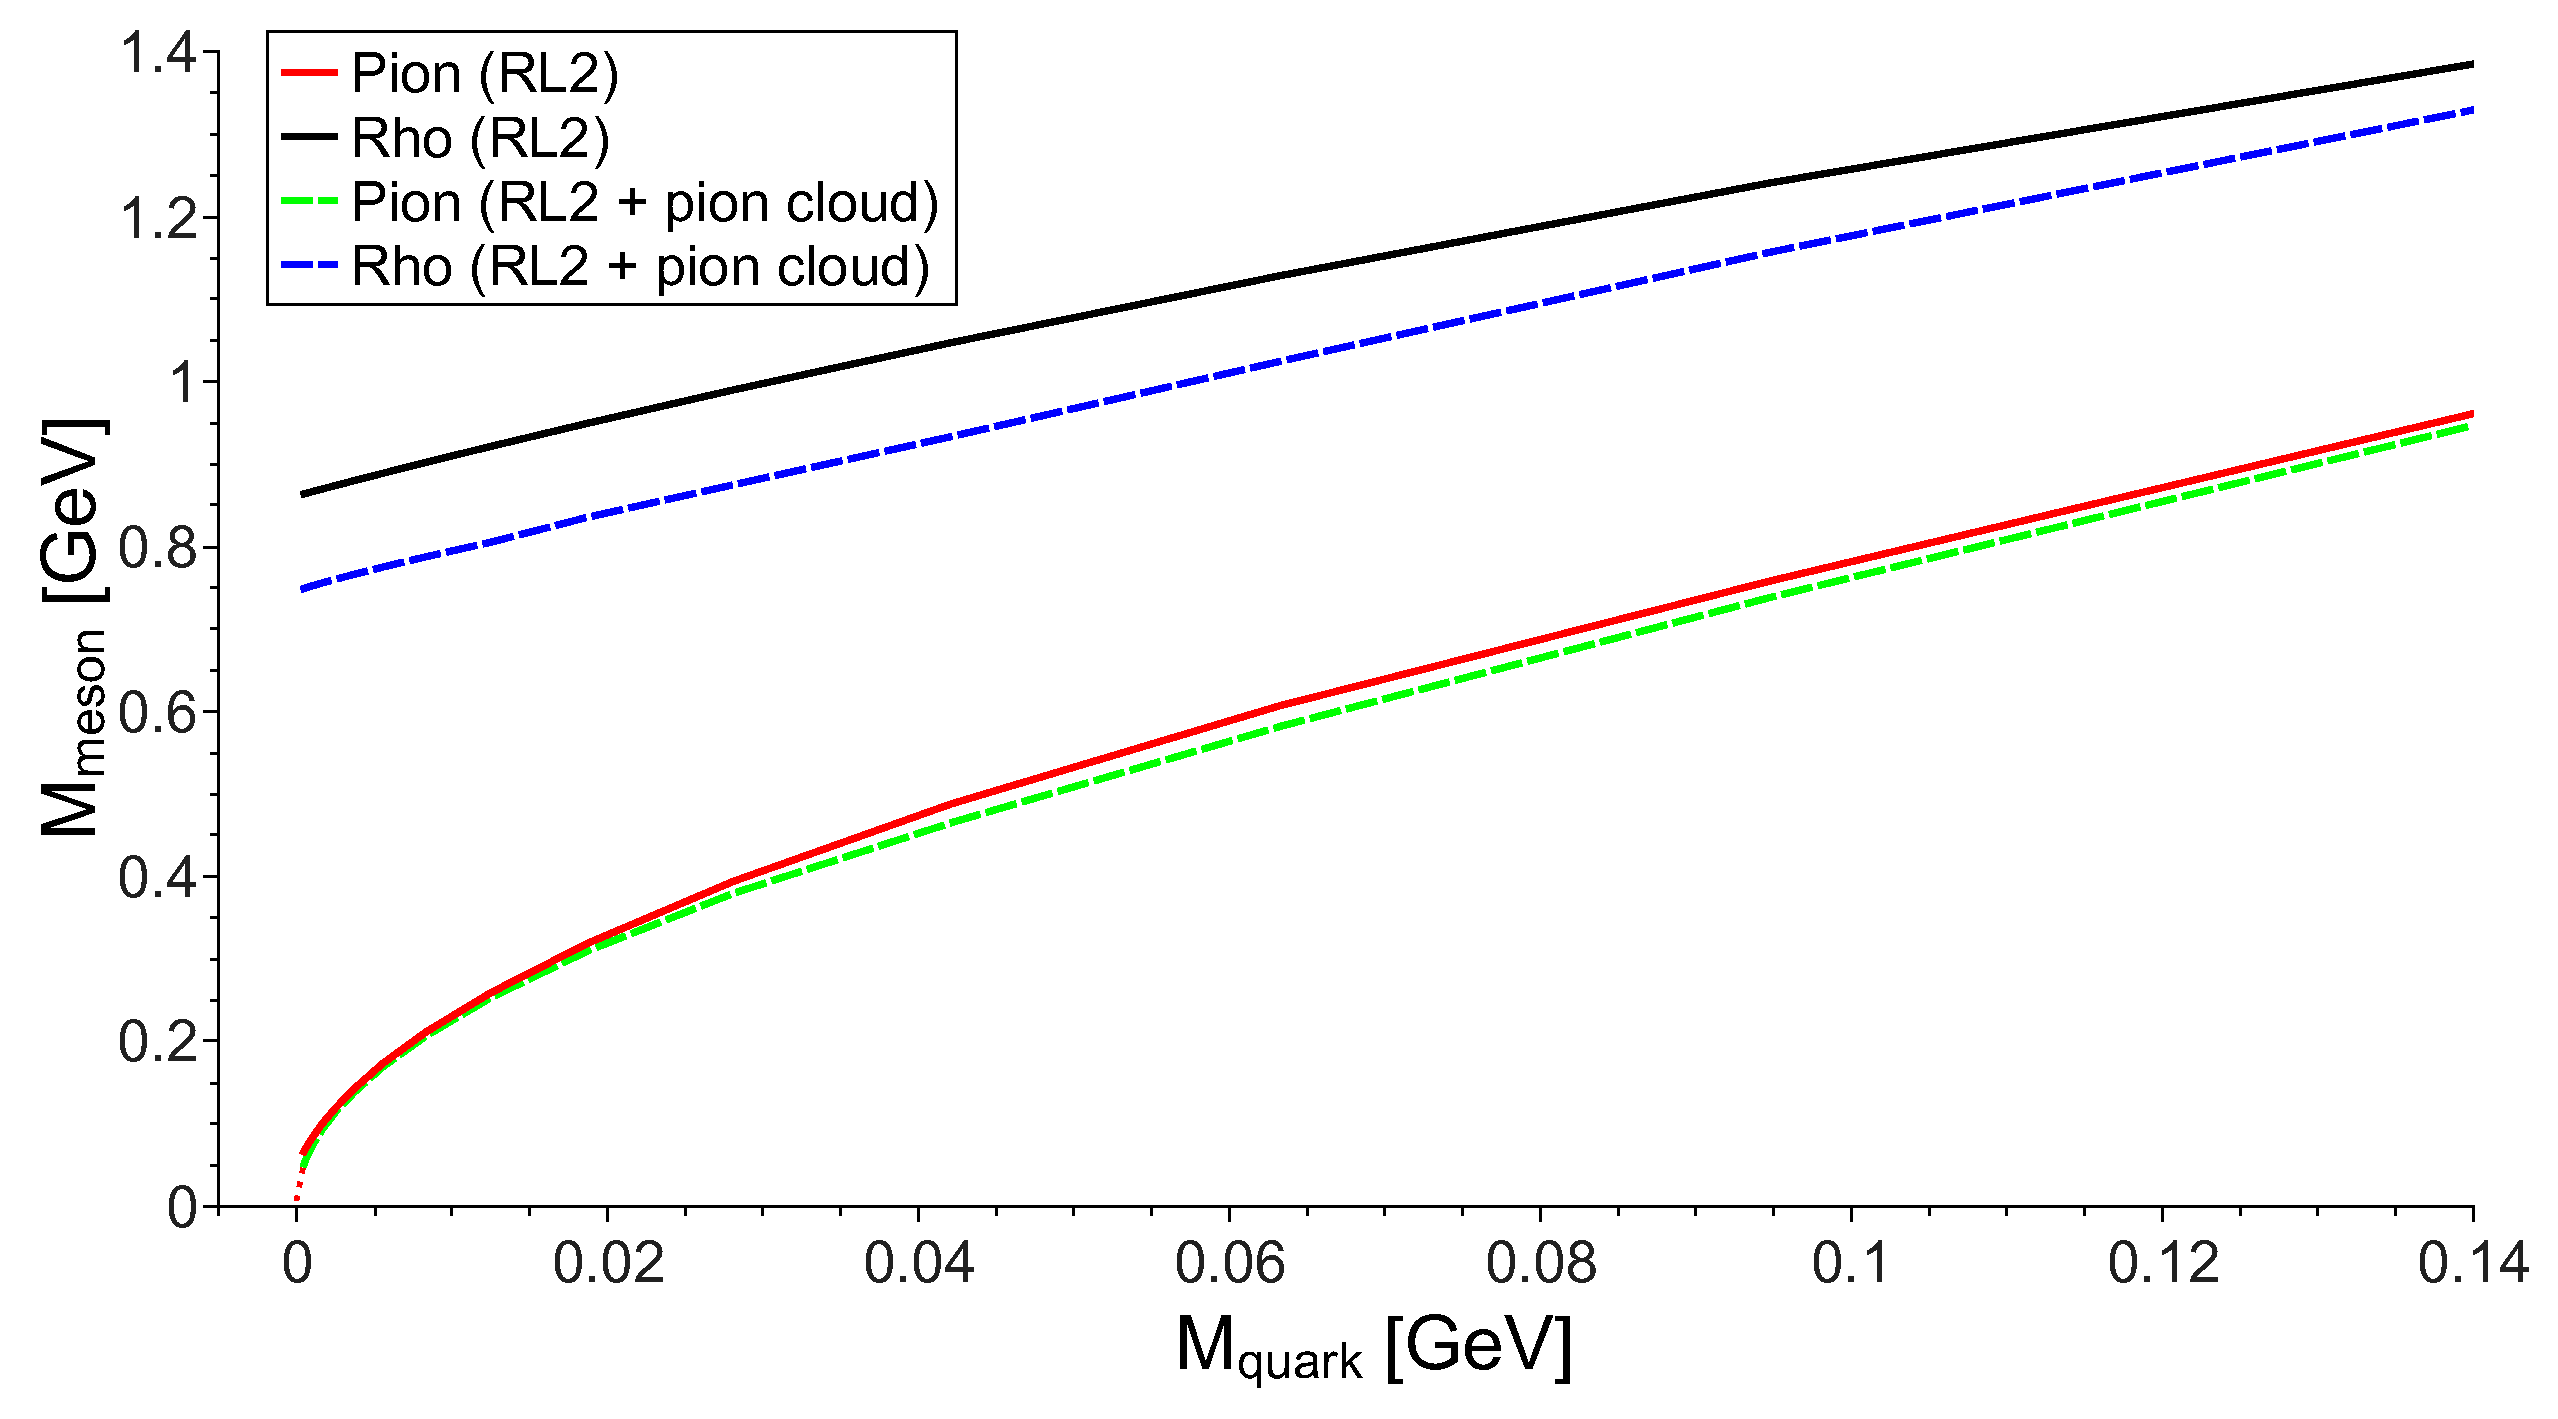
\includegraphics[width=0.99\textwidth]{figures/GMOR_Pi} 
\caption{\footnotesize Masses of pion and rho as functions of quark mass. The Gell-Mann-Oakes-Renner relation is indicated. }\label{fig:GMOR}
\end{center}
\end{figure}
representing effective single gluon exchange must change its parameters $\Lambda$ and $\eta$ in order to incorporate the withdraw of the hadronic contribution into the explicit part $ K^{pion}$. 
The parameters are $\Lambda=0.84$ and $\eta=1.8$ as given in Table. \ref{tab:RL_params}. It is also interesting to perform the calculations with and without the pion cloud effect switched on to draw some insights on size on unquenching effects. The results on meson masses, decay constant and the chiral condensate are given on Table. \ref{tab:masses_mesons}. The general trend is that inclusion of the pion cloud effect provides lighter spectrum in comparison to RL2 by generating a downwards shift in average 70-130 MeV.  \\

The complete interaction kernel consisting of
the rainbow-ladder gluonic diagram and the pion exchange diagram does
satisfy the axial-vector Ward-Takahashi identity. This can be demonstrated 
analytically \cite{Fischer:2007ze,Fischer:2008wy} and holds even with the
approximation of the exchanged pion's Bethe-Salpeter amplitude. As a result,
using this interaction kernel one obtains a pseudoscalar Goldstone boson
in the chiral limit and the holding Gell-Mann-Oakes-Renner relation \cite{Fischer:2007ze,Fischer:2008wy} as it shown on Fig. \ref{fig:GMOR}. 
Since this truncation scheme does not contain the t-channel two-pion exchange diagram for the $\rho$ to decay into pions, we do not observe
the specific behaviour of the rho mass as the pion mass reaches threshold $m_\pi>m_\rho/2$, due to the opening of a decay channel \cite{Allton:2005fb}. The impact on baryon masses will be considered in the next chapter. \\

%\subsection*{Photon-quark vertex}
\section{Baryons}
\label{sec:results}

\begin{table*}[t]
 \begin{center}
 \small
\renewcommand{\arraystretch}{1.2}
  \begin{tabular}[h]{|c||c|c|c|c|}\hline
  [GeV]     &  RL1     & RL2      & RL2 + $\pi$ & Exp. \\ \hline\hline
 $m_\pi$  	& 0.138 (1)& 0.144 (1)& 0.138 (1)   & 0.140\\ \hline
 $f_\pi$  	& 0.093 (1)& 0.098 (1)& 0.093 (1)   & 0.093\\ \hline
 $\langle q\bar{q}\rangle^{1/3}_{\mu=19 \,\text{GeV}}$
          	& 0.281 (2)& 0.300 (3)& 0.280 (3)    &      \\ \hline\hline
 $m_N$      & 0.94 (1) & 1.01 (3) & 0.86 (1)    & 0.94 \\ \hline
 $m_\Delta$ & 1.23 (1) & 1.36 (1) & 1.30 (3)    & 1.23 \\ \hline
\end{tabular}
\caption{Nucleon and Delta masses as well as pion mass, decay constant and the chiral condensate 
using the rainbow-ladder truncation only (RL1),
rainbow-ladder with the refitted effective interaction (RL2) and including the pion 
cloud corrections corrections (RL2 + $\pi$). 
We give the central value of the bands corresponding to a variation of 
$\eta$ between $1.6 \le \eta \le 2.0$ with the halfwidth of the bands added in brackets. 
We compare also with experimental values.\label{tab:masses}}
 \end{center}
\end{table*}

\begin{figure*}[t]
\begin{center}
  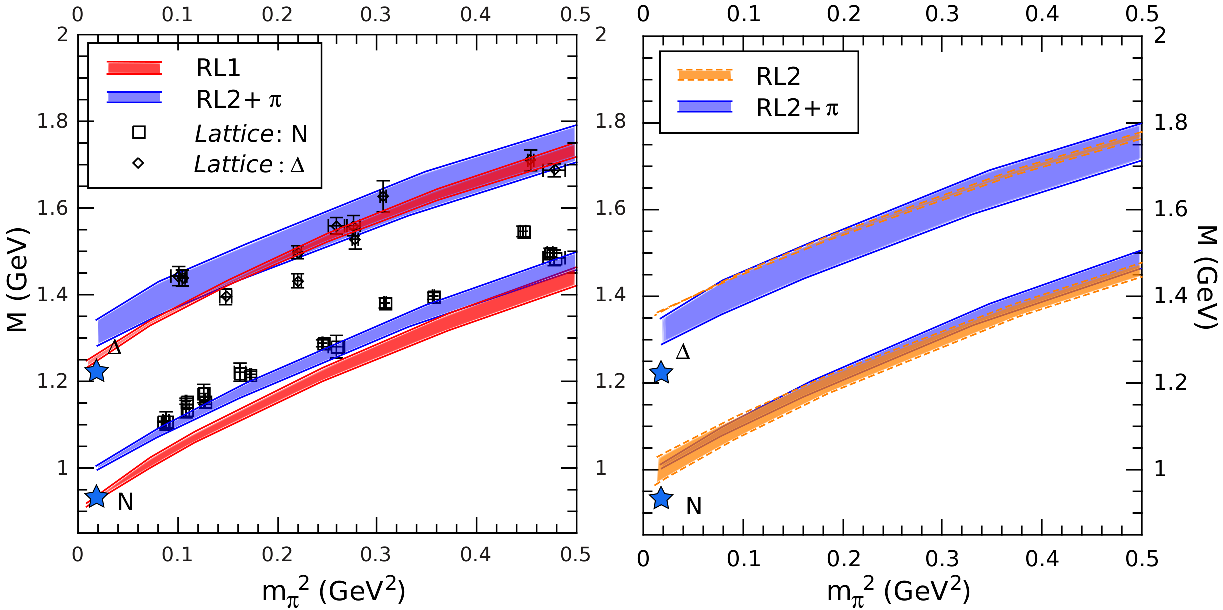
\includegraphics[width=0.99\textwidth]{figures/eta-bands}
 \end{center}
 \caption{Evolution of the nucleon and delta mass with respect to the pion mass squared. \textit{Left panel}: We plot the results for pure RL1 and for RL2 with pion exchange. We also compare with a selection of (unquenched) 
lattice data \cite{Alexandrou:2006ru}-\cite{Gattringer:2008vj}. \textit{Right panel}: We compare the results for RL2 only and RL2 with pion exchange. Stars denote the physical nucleon and delta mass.
The shaded bands correspond to a variation of the interaction parameter $\eta$ between
$1.6 \le \eta \le 2.0$, with $\eta=1.6$ corresponding to the upper limit of the bands.}\label{fig:mass_panel}
\end{figure*}

To proceed with the calculations we must fix the two parameters $\Lambda$ 
and $\eta$ of the interaction as well as the 
current-quark masses. This is conveniently done by using the 
experimental values for the pion decay constant $f_\pi$ and the pion mass $m_\pi$
as benchmark. The pion decay constant is largely insensitive to the 
current quark mass, which is consequently fixed by the physical pion mass.
On the other hand, the parameter $\Lambda$ corresponds to an interaction 
scale, and is therefore in one-to-one relation with $f_\pi$. Furthermore,
it has been noted that the pion decay constant can only be reproduced by 
a range of values of $\eta$ between $1.6$ and $2.0$ (see, e.g. 
\cite{Eichmann:2011vu,Krassnigg:2009zh}). 
For the pure RL interaction $\widetilde{K}^{RL}$ the resulting values for $\Lambda$ and the quark mass
are $\Lambda=0.72$~GeV and $m_{u/d}(\mu^2)=3.7$~MeV; we denote this case by RL1.
Since the pion back-reaction is not taken into account explicitly in this case,
its effects are, to some extent, encoded implicitly in the parameters (in particular the scale) 
of the interaction. This is different for the pion corrected kernel 
$\widetilde{K} = \widetilde{K}^{RL}-\widetilde{K}^{pion}$. Since pion cloud effects are 
now treated explicitly, $\widetilde{K}^{RL}$ describes 
the interactions in the bound state's quark-core only. As a result, the 
interaction range of this part of the kernel (in coordinate space) is expected to decrease, which in turn means that 
$\Lambda$ should increase \cite{Thomas:1981vc}. This is indeed what we observe: for the 
pion-corrected kernel we need $\Lambda=0.84$~GeV to reproduce $f_\pi$ with 
$\eta \in [1.6,2.0]$. The quark mass $m_{u/d}(\mu^2)=3.7$~MeV remains the same.
We use the label RL2 for the RL part of this truncation. 
The renormalisation scale in all cases is chosen to be $\mu^2= (19 \,\mbox{GeV})^2$.

\subsection*{Nucleon and Delta masses and Sigma terms}
The calculated masses of the Nucleon and the Delta, with and without the 
pion-exchange kernel, are shown in Tab.~\ref{tab:masses}. In the RL1 framework
one observes very good agreement with the experimental 
mass values. However, as shown in Ref.~\cite{Eichmann:2011vu,Eichmann:2011pv}, the 
internal structure of the nucleon as probed by electromagnetic as well as axial 
and pseudoscalar currents is not well represented at low momenta due
to missing explicit pion cloud effects. These are included (within the limits of 
our truncation) in the RL2 + $\pi$-calculation. For comparison we also display 
results for the purely gluonic rainbow-ladder part of this truncation (RL2), which
represents a quark-core calculation of the nucleon mass with stripped pion cloud.
As a result we find substantial pion cloud effects in the nucleon. Compared with 
the quark-core part (RL2) the nucleon mass is reduced by about $150$ MeV in the 
full calculation (RL2+$\pi$). Comparing RL2+$\pi$ with RL1, which both reproduce
the physical pion mass and decay constant we still find pion cloud effects of the
order of $80$ MeV. This sizable mass shift for the nucleon at the physical
point agrees qualitatively with other estimates in the literature, see e.g. 
\cite{Young:2002cj} and references therein. The corresponding mass shift in the
$\Delta$-isobar is much smaller and behaves differently. Comparing RL2 and RL2+$\pi$
we find a decrease of the $\Delta$-mass by about $60$ MeV, which is less than half
the size of the corresponding shift in the nucleon. However, when comparing with
RL1, we even find an increase in the $\Delta$-mass by about $70$ MeV. This is a
result of the different interaction scale $\Lambda$ in the two setups, which
was necessary to reproduce the physical pion decay constant correctly. As a result
we find a mass shift of different sign for the $\Delta$ than for the nucleon. \\

The evolution of the baryon masses as a function of $m_\pi^2$ (or, equivalently, 
with respect to the current-quark mass), is displayed in Fig.~\ref{fig:mass_panel},
where we also display corresponding lattice data \cite{Alexandrou:2006ru}-\cite{Gattringer:2008vj}.
In general, we observe that the inclusion of pion cloud effects increases the mass 
splitting between the nucleon and the $\Delta$ considerably. Although the size of 
this increase may be too large, its qualitative behavior is in agreement with
well-known results in the literature \cite{Thomas:1981vc}. Including the pion
cloud effects, the excellent agreement of the pure rainbow-ladder calculation RL1
with experiment is spoiled and we are left with discrepancies for the nucleon
and the $\Delta$ on the ten percent level. Whereas the mass evolution for the 
$\Delta$ is not too far away from the corresponding lattice results, the one
for the nucleon is shifted by 10-20 percent for all pion masses, although the slope 
of the evolution is more or less correct. \\

In general, however, the quantitative discrepancies of our approach with the lattice 
results indicate missing structure such as gluon self interaction effects in the
two-body kernels (see \cite{Fischer:2009jm} for a study of these in the meson 
sector), genuine three-body interactions (also mediated by gluon self interaction
contributions) and potential deficiencies in our pion exchange kernel. This
needs to be further explored in future work.  \\

An observable effect of the slope of the mass-evolution curve close to the physical
point is given by the nucleon and delta sigma terms. In our approach, these are
trivially obtained using the Feynman-Hellman theorem
\begin{equation}
 \sigma_{\pi X}=m_q\frac{\partial M_X}{\partial m_q}\,,
\end{equation}\label{eq:sigma_terms}
where $m_q$ is the current-quark mass, $M_X$ is the baryon mass and the derivative 
is taken at the physical quark mass. For the nucleon we obtain 
\begin{eqnarray}
\sigma_{\pi N} &=& 30 (3)~\mbox{MeV (RL1)}, \nonumber\\
\sigma_{\pi N} &=& 26 (3)~\mbox{MeV (RL2)}, \nonumber\\
\sigma_{\pi N} &=& 31 (3)~\mbox{MeV (RL2+$\pi$)} \label{FH1}
\end{eqnarray}
for RL1, RL2 without and RL2 with pion exchange, respectively. Likewise, we obtain 
for the delta 
\begin{eqnarray}
\sigma_{\pi \Delta} &=& 24 (2)~\mbox{MeV (RL1)}, \nonumber\\
\sigma_{\pi \Delta} &=& 23 (3)~\mbox{MeV (RL2)}, \nonumber\\
\sigma_{\pi \Delta} &=& 24 (3)~\mbox{MeV (RL2+$\pi$)}\,. \label{FH2}
\end{eqnarray}
For the pion-nucleon case both of our values using physical parameters (RL1 and RL2+$\pi$) 
are slightly below the lower bound of a range of recent lattice 
results \cite{Shanahan:2012wh,Alvarez-Ruso:2013fza,Bali:2013dpa}. From a comparison of the
quark core calculation RL2 with RL2+$\pi$ we infer that about twenty percent of the nucleon
sigma term are generated by pion cloud effects. For the $\Delta$ this fraction is considerably 
smaller and our results in general are about 30 \% lower than available model 
results \cite{Lyubovitskij:2000sf,Cavalcante:2005mb}. \\

Within certain limits, the slope can be influenced by the choice of the model
parameters as reflected in the numbers in brackets given in (\ref{FH1}) and (\ref{FH2}).
However, as mentioned above, in order to study the mass evolution of the system 
and the resulting sigma-terms in more detail, one should include 
the effects of the gluon self-interaction in the two-body and three-body 
correlations, since these may have a significant impact \cite{Fischer:2009jm}. 

\subsection*{Internal composition}\label{subsec:internal_composition}
Some insight into the internal structure of the baryon can be gained by 
studying the relative importance of the different partial-wave sectors. 
As shown in \cite{Eichmann:2009qa,Eichmann:2009en,SanchisAlepuz:2011jn}, 
Poincar\'e covariance enforces that in our framework baryons are composed, 
in principle, by s-, p- and d-wave components for spin-$\frac{1}{2}$ 
particles and s-, p-, d- and f-wave components for spin-$\frac{3}{2}$
particles. Therefore, one \textit{cannot} restrict the partial-wave 
composition in a covariant way and it is the dynamics what 
dictates the contribution of these components to a given state. Moreover, 
in the case of the nucleon, the flavor part of the Faddeev amplitude contains 
a mixed-symmetric and a mixed-antisymmetric term, as dictated by symmetry. 
Each of these is accompanied by a spin-momentum part; these are not identical
but related to each other. In our calculation we take all these contributions
into account. \\

Form factors are observables which are expected to be more sensitive to the internal structure of the baryon. In particular, the $N\Delta\gamma$ transition \cite{Eichmann:2011aa} as well as the electromagnetic $\Delta$-baryon form factors \cite{Sanchis-Alepuz:2013iia} show a qualitatively different behavior when the angular-momentum content is artificially restricted. For this reason, we have calculated the contribution of the different partial-wave sectors to the normalization of the $N$ and $\Delta$ amplitudes when the pion corrections are or are not included, see Table \ref{tab:PartialWaveContributions}. In the case of the nucleon we average the contributions from the mixed-symmetric and mixed-antisymmetric terms. The angular-momentum composition of the state is not, nevertheless, the only element determining the form factors. The coupling of the photon (in case of electromagnetic form factors) and pion cloud plays an important role and is likely to be the dominant correction for, e.g., the baryon's charge radius and magnetic moment. This is, however, beyond the scope of this work.
\begin{table*}[t]
 \begin{center}
 \small
\renewcommand{\arraystretch}{1.2}
  \begin{tabular}[h]{|c||c|c|c|}\hline
Nucleon &  RL1  &  RL2	        &	RL2 + $\pi$   \\ \hline\hline
 s-wave & 65.9  &  75.0 (1)		&	75.0 (1)     \\ \hline
 p-wave & 33.0  &  24.1 (3)		&	24.2 (0)     \\ \hline
 d-wave &  1.1  &   0.9 (1)		&	 0.8 (1)  \\ \hline
\end{tabular}\hspace{1cm}
  \begin{tabular}[h]{|c||c|c|c|}\hline
  Delta &  RL1 &  RL2	&	RL2 + $\pi$ \\ \hline\hline
 s-wave & 56.5 &  61.4 (15)	&	60.5 (14) \\ \hline
 p-wave & 39.9 &  31.0 (6)	&	31.1 (11) \\ \hline
 d-wave & 3.4  &  7.4 (20)	&	 8.1 (23) \\ \hline
 f-wave & 0.2  &  0.2 (1)	&	 0.3 (2) \\ \hline
\end{tabular}
\caption{Contribution in \% of the different partial wave sectors, at $m_{\pi}=138$~MeV, 
to the normalization of the Faddeev amplitudes for the Rainbow-Ladder kernel only (RL1) 
and for RL2 including pion cloud effects (RL2+$\pi$). As before, the numbers in brackets 
reflect the change of the results under variation of the interaction parameter $\eta$ 
between $1.6 \le \eta \le 2.0$. For RL1 this variation is very small and therefore no 
range is given. \label{tab:PartialWaveContributions}}
 \end{center}
\end{table*} \\

Accepting the aforementioned caveats, it is nevertheless interesting to 
discuss the internal structure of the nucleon and $\Delta$ displayed in 
Tab.~\ref{tab:PartialWaveContributions}. Let us begin by analyzing 
the nucleon results. From comparison of our three setups it is clear 
that the inclusion of pion cloud effects induce only slight but potentially
significant changes in the angular-momentum content of the nucleon. These
are, however, not induced directly by the pion exchange term (cp. RL2 with
RL2+$\pi$), but by the accompanying change in the interaction scale of the
core rainbow-ladder contribution. In coordinate space this change of scale 
corresponds to a decrease of the core size, resulting in a larger s-wave 
component. This new balance is hardly affected by the explicit pion contributions.
It remains to be seen, how this affects the form factors of the nucleon.
Here, possible quantitative corrections will be dictated by the direct 
pion-photon interaction and may be large in the magnetic moments and the neutron
form factors at low momentum transfer \cite{Eichmann:2011vu}. \\

The case of the $\Delta$ is slightly different from the nucleon. Also here, the
main effects are generated by the modified interaction range of the core
rainbow-ladder contribution. The increase of the s-wave contributions as compared
to p-wave is less severe than in the nucleon case. Instead, the d-wave contributions
increase significantly with more than doubling their relative size as compared to
pure rainbow-ladder. This might have a significant impact in those form factors 
that measure the deformation of the $\Delta$-baryon, {\it i.e.} the electric quadrupole 
and the magnetic octupole \cite{Sanchis-Alepuz:2013iia}. Especially the latter 
one is small and therefore may be very sensitive to changes in the baryon internal 
structure.

\section{Pion Form Factor}
The fact that hadrons have a substructure was realized more 50 years ago in early SLAC deep inelastic scattering experiments \cite{9780471887416}. Later on the parton model was suggested by Bjorken and Paschos as an interpretation of these large momentum transfer experiments. In the essence of the parton model lies the idea that the hadron consists of free point-like fermions, partons. After the discovery of asymptotic freedom of QCD, the calculation of hadronic observables at large momentum transfer lead these partons to be identified with quarks and gluons. However, at low energy momentum or large scales, the QCD running coupling is large so that the high energy picture of the parton model consisting of weakly interacting quarks and gluons should not be extrapolated to these limits. At this low energy scale the non-pertubative effects play a major role and therefore cannot be avoided. 

\begin{figure}[!h]
\begin{center}
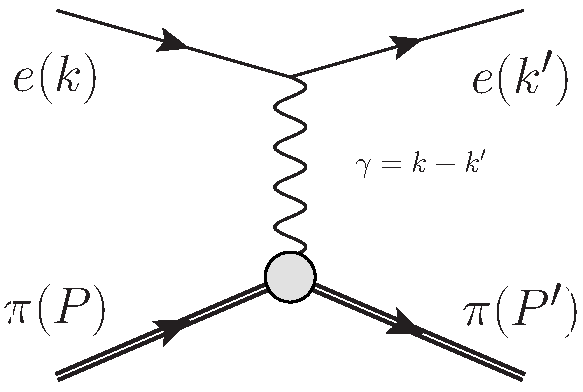
\includegraphics[width=0.55\textwidth]{figures/FF_gen} 
\caption{\footnotesize One-photon exchange pion elestic scattering. }\label{fig:FF_gen}
\end{center}
\end{figure}

The electron-hadron scattering experiments are well-proven technique since the electromagnetic part is well known. In this thesis we will focus on the pion as the target of scattering. The simplified picture of the corresponding experiment is given on Fig. \ref{fig:FF_gen}. The angular distributions of the cross section takes the form:
\beqa
	\frac{d\sigma}{d\Omega} =  \left( \frac{d\sigma}{d\Omega} \right)_{point-like} |F_\pi(q^2)|^2 \;,
	\label{pion:crosssection}
\eeqa
where $q=k-k^{\prime}$ is the momentum energy transferred between the electron and the pion. For the convenience purpose we consider the variable $Q^2 = - q^2$. The $F_\pi(q^2)$ is the pion electromagnetic form factor. For a static targets the form factor is given by Fourier transform of normalized charge distribution $\rho(\textbf{x})$:
\beqa
	F(\textbf{q}) = \int d^3x \rho(\textbf{x}) exp(i\textbf{q}\textbf{x})
	\label{pion:3d_FF}
\eeqa
If the momentum transfer is small we can expand the exponential in Eq. (\ref{pion:3d_FF}), obtaining:
\beqa
	F(\textbf{q}) = 1 - \frac{1}{6}\langle r^2 \rangle|\textbf{q}^2| + ...
\eeqa
As we see from the expansion the mean square radius of pion charge distribution is given by:
\beqa
\langle r^2 \rangle = - 6 \frac{dF(Q^2)}{dQ^2}
\eeqa
So the low momentum transfer electron-pion scattering measures only the mean square radius of the charge cloud of the pion. And this is expectable since the long wavelength virtual photon can only resolve the size of pion, but not its substructure. \\

According to Eq. (\ref{pion:crosssection}), the scattering on the pion as a spinless particle, in fully described by its form factor $F_\pi(Q^2)$. However we know that pion-photon vertex must be a Lorentz four-vector since photon is able to couple to it. This deduce the view of pion-photon vertex to the form:
\beqa
	(P^{\prime} + P)_\mu F_\pi(Q^2)
	\label{pion:FF_vertex}
\eeqa
From another side the pion-photon vertex can be written in a general form as:
\beqa
	\left\langle \pi(P^{\prime}) |J_\mu | \pi(P) \right\rangle\;,
	\label{pion:current_vertex}
\eeqa
where $\left\langle \pi(P) |\right. $ is the wave function of incoming pion, $\left. | \pi(P) \right\rangle $ is the wave function of outgoing pion and $J_\mu$ is pion's electromagnetic current. Obviously the Eq. (\ref{pion:FF_vertex}) is equal to Eq. (\ref{pion:current_vertex}), thus providing the route to calculate pion form factor:
\beqa
	\left\langle \pi(P^{\prime}) |J_\mu | \pi(P) \right\rangle = (P^{\prime} + P)_\mu F_\pi(Q^2)
	\label{pion:FF_relation}
\eeqa
So in order to obtain the electromagnetic pion form factor $F_\pi(Q^2)$ we need to know pion wave-function $\left. | \pi(P) \right\rangle$, which explicit view was established in Chapter \ref{chap:BSE} and is given by:
\beqa
	\left. | \pi(P) \right\rangle = \chi(k;P) = S(k + P/2)\Gamma(k;P)S(k - P/2)
\eeqa
and pion's electromagnetic current $J_\mu$. The current can be obtained by "gauging" the quark-quark scattering kernel $K$. \\

A description of systematic approach how to couple external gauge field was given by \cite{Sanchis-Alepuz:2013iia}. Shortly, the evolution of two-body quark system is given by the amputated version of scattering matrix $T^{(2)}$. Thus the scattering matrix $T$ can be obtained by solving the following Dyson equation:
\begin{equation}
\displaystyle T=-iK-iKG_0T
\label{Gauging_1}
\end{equation}
where $G_0$ is the disconnected product of two full quark propagators and $-iK$ is the two-quark interaction kernel. When the two-quark system forms a bound state, the scattering matrix develops a pole at $P^2=-M^2$, and can be defined as:
\begin{equation}
\displaystyle T^{(2)}\approx \frac{\Gamma \bar \Gamma}{P^2+M^2}
\label{Gauging_2}
\end{equation}
Substituting \ref{Gauging_2} in \ref{Gauging_1} and keeping only the singular term, we arrive at the \BSE for two quark bound state:
\begin{equation}
\displaystyle \Gamma = -iKG_0\Gamma,\:\:\:\:\ or \:\:\:\: iK^{-1}\Gamma = G_0\Gamma, \:\:\:\: or \:\:\:\: i\bar{\Gamma}K^{-1}=\bar{\Gamma}G_0
\label{Gauging_3}
\end{equation}
Then a systematic procedure of coupling to external gauge field, introduced in \cite{Kvinikhidze:1998xn}, gives for $T^{(2)}$:
\begin{equation}
\displaystyle T^\mu = T(iK^{-1} K^\mu K^{-1} + G_0^\mu)T
\label{Gauging_4}
\end{equation}
The bound state electromagnetic current $J^\mu$ can be expressed at the pole by:
\begin{equation}
\displaystyle T^{(2), \mu} \approx \frac{\Gamma_f}{P^2_f+M^2_f}J^\mu\frac{\bar \Gamma_i}{P^2_i+M^2_i}
\label{Gauging_5}
\end{equation}
Substituting \ref{Gauging_5} in \ref{Gauging_4} and using \ref{Gauging_3} we get:
\begin{equation}
\displaystyle J^\mu= \Gamma_f (-iG_0 K^\mu G_0 + G_0^\mu) \Gamma_i
\label{pion:pion_EM_current}
\end{equation} 

In case of rainbow-ladder single-gluon exchange the interaction kernel involves only gluon, so the first term $K^{\mu}=0$ because gluon does not couple to photon directly. So only the second term in Eq. (\ref{pion:pion_EM_current}) contributes to the current and the pion form factor is given by following diagram:
\begin{figure}[h]
\centering
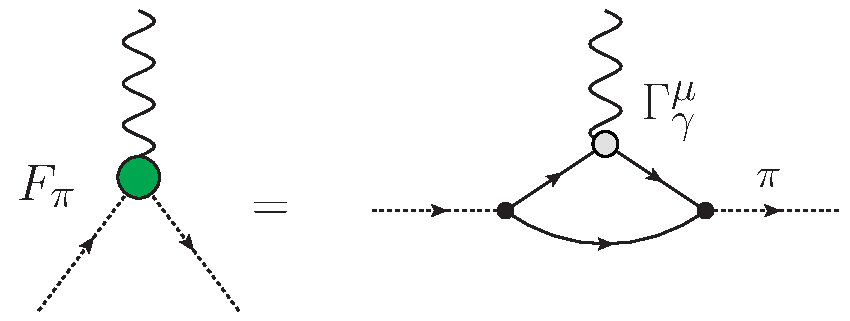
\includegraphics[width=0.7\textwidth]{figures/FF_RL}
\caption{\label{fig:FF_RL}\footnotesize Diagrams that contribute to pion form factor in case of rainbow-ladder single gluon exchange. All internal vertexes and propagators are dressed.}
\end{figure} \\

In case of pion cloud effect included, the gauging of the kernel is no longer zero $K^{\mu}\neq0$, since the kernel consists of quark-pion vertex and propagating pion and it is possible to couple a photon to the exchanging pion or to the quark-pion vertex. This fact generates two additional diagrams for the pion form factor. So they are given by diagrams in Fig. \ref{fig:FF_with_pi}. \\
\begin{figure}[h]
\centering
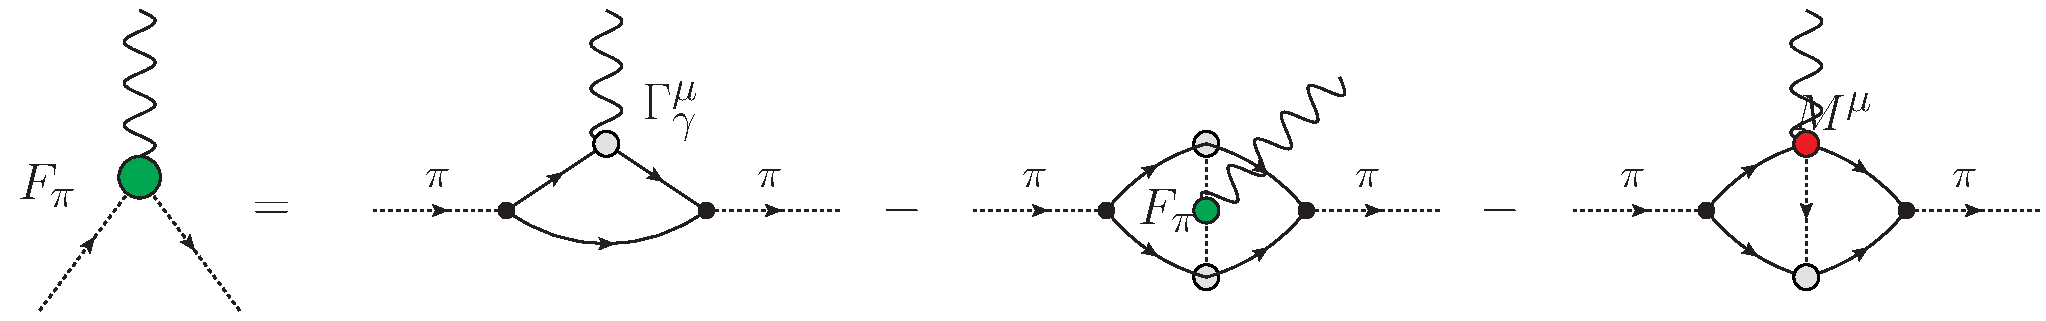
\includegraphics[width=0.99\textwidth]{figures/FF_with_pi}
\caption{\label{fig:FF_with_pi}\footnotesize Diagrams that contribute to pion form factor in case of pion cloud included. The second diagram (pion self-coupling) involves the pion form factor itself. The third diagram (seagull) involves the quark-pion-photon 4-vertex. All internal vertexes and propagators are dressed.}
\end{figure}
In comparison to rainbow-ladder the calculation become more complicated. The second diagram involves pion form factor in itself, so it requires to perform a self-consistent, iterative calculation, additionally complicated by two-loop integration. \\

Generally the pion-photon vertex depends on three momenta: $P_-$ - the initial momentum, $P_+$ - the final momentum and $Q$ - the momentum transferred. However, the momentum conservation $P_- + P_+ + Q = 0$ implies that only two momenta are independent. We choose the independent momenta to be the incoming photon momenta $Q$ and central-mass collision momentum $P$. The initial and final meson momenta can be written in terms of $Q$ and $P$ as $P_-=P-\frac{Q}{2}$ and $P_+=P + \frac{Q}{2}$, respectively. The condition of elastic scattering imposes additional constraints on $Q$ and $P$: $P_-^2=P_+^2=-m^2_{\pi}$,  $P^2=-\frac{Q^2}{4}-m^2_{\pi}$, so that only one remains independent. We use the specific momentum frame: 
\beqa
	Q_\mu &=& (0,0,Q,0)\\
	P_\mu &=& (0,0,0,P)\;,
\eeqa
where $Q$ and $P$ defined as:
\beqa
	Q &=& (Q^2)^{1/2}\\
	P &=& i\left( m^2_{\pi} + \frac{Q^2}{4}\right) ^{1/2}
\eeqa
After the frame is set we proceed to define the internal momenta routing for all diagrams in Fig. \ref{fig:FF_RL} and Fig. \ref{fig:FF_with_pi}.

\subsection*{Diagram A: Rainbow-ladder}
The first diagram A is given on Fig. \ref{fig:FF_A}.
\begin{figure}[h]
\centering
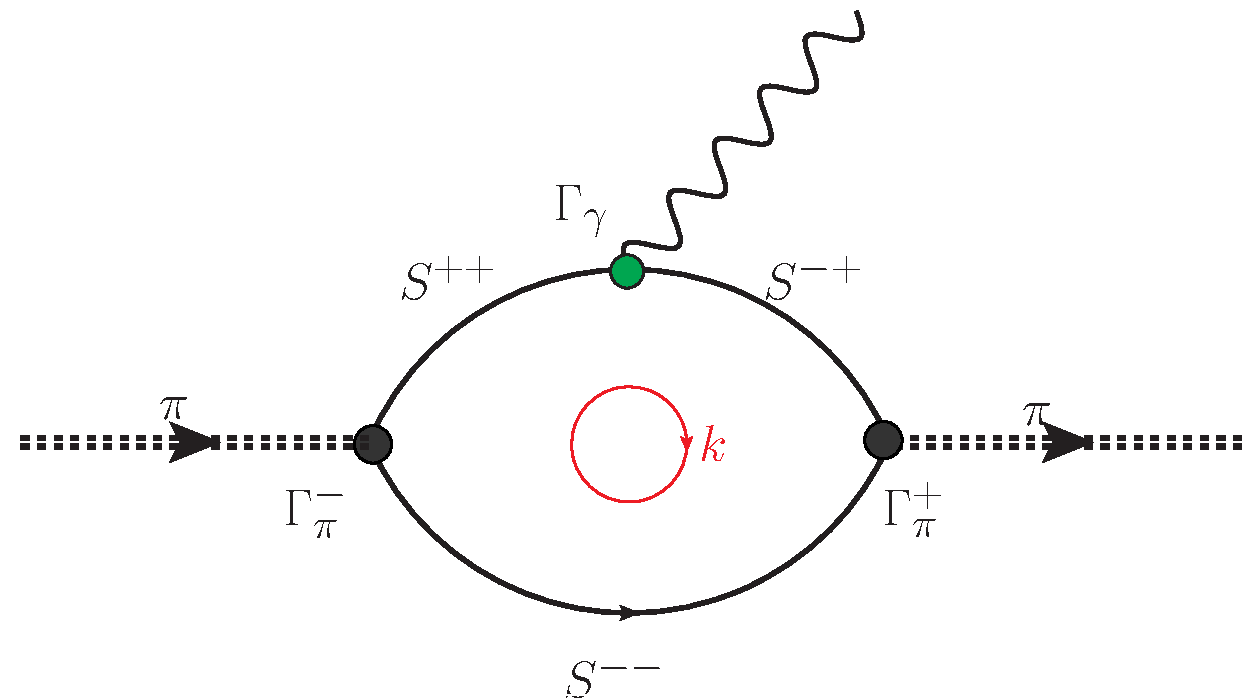
\includegraphics[width=0.7\textwidth]{figures/FF_A}
\caption{\label{fig:FF_A}\footnotesize The first diagram, common for the rainbow-ladder single gluon exchange and pion cloud effect. All internal vertexes and propagators are dressed.}
\end{figure}
According to the momenta routing choice the dressed vertexes and propagators have to evaluated on the following momenta:
\beqa
	\Gamma_{\pi}^-(k+Q/4,P_-)\;, & S^{++}(k + Q/2 + P/2) \\
	\Gamma_{\pi}^+(k-Q/4,P_+)\;, & S^{-+}(k - Q/2 + P/2) \\
	\Gamma_{\gamma}(k-P/2,Q)\;, & S^{--}(k - Q/2 - P/2)
\eeqa
where $k$ is integration momentum. The explicit notation of the corresponding to diagram A integral is following:
\beqa
	\frac{P_{\mu}}{P^2} \int \frac{d^4k}{(2\pi)^4} \Tr \left[ \Gamma_{\pi}^+ S^{-+} i\Gamma_{\gamma}^{\mu} S^{++} \Gamma_{\pi}^- S^{--} \right] 
\eeqa
Note that this notation is same in both cases - rainbow-ladder gluon exchange only or with pion cloud included.

\subsection*{Diagram B: Pion self-coupling}
The second diagram B illustrated on Fig. \ref{fig:FF_B}.
\begin{figure}[h]
\centering
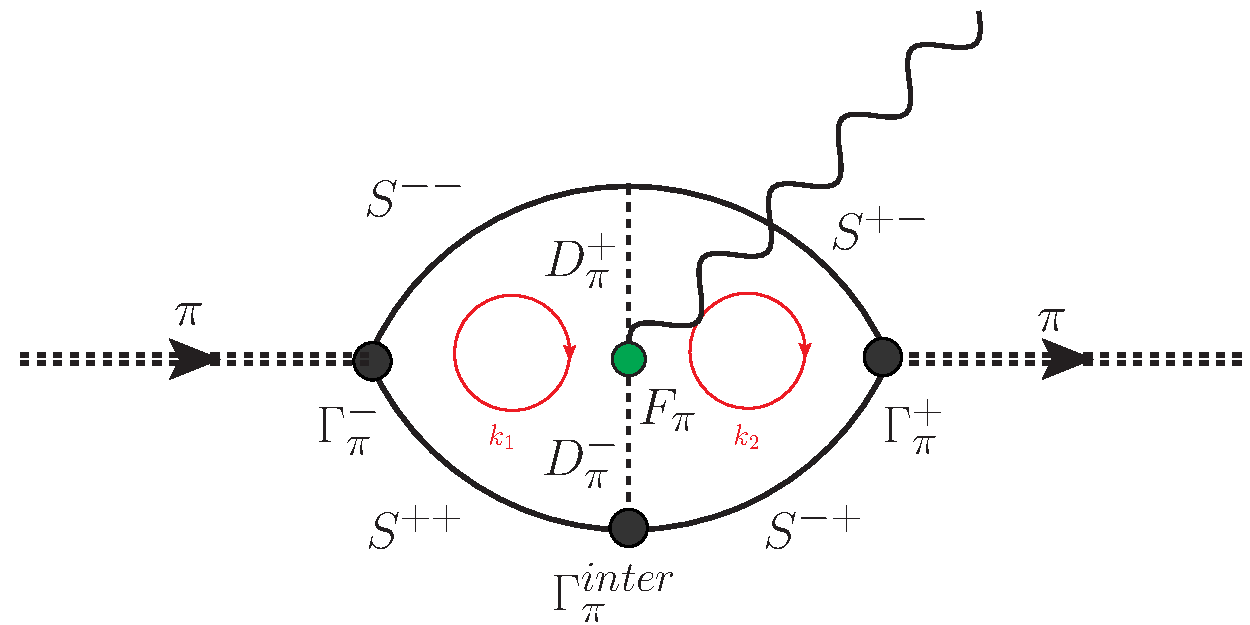
\includegraphics[width=0.7\textwidth]{figures/FF_B}
\caption{\label{fig:FF_B}\footnotesize The second diagram (pion self-coupling), which involves the pion form factor itself. All internal vertexes and propagators are dressed.}
\end{figure}
The momenta routing choice for the dressed vertexes and propagators reads as:
\beqa
	&\Gamma_{\pi}^-(k_1,P_-)\;, & S^{--}(k_1 - Q/4 - P/2)\\
	&\Gamma_{\pi}^+(k_2,P_-)\;, & S^{+-}(k_2 + Q/4 - P/2)\\
	&\Gamma_{\pi}^{inter}(\frac{k_1 + k_2 + P}{2})\;, & S^{-+}(k_2 - Q/4 + P/2)\\
	&F_\pi(Q^2)\;, & S^{++}(k_1 + Q/4 + P/2)\\
	&D_{\pi}^-(-Q/2 - k_1 + k_2)\;, & D_{\pi}^+(Q/2 - k_1 + k_2)
\eeqa
where $k_1$ and $k_2$ denotes integration momenta, flowing clock-wise as show by red contours on the diagram. $\Gamma_{\pi}^{inter}(\frac{k_1 + k_2 + P}{2})$ is the Bethe-Salpeter pion wave function, given in chiral approximation $\Gamma_{\pi}^{inter}(p) = \frac{B(p)}{f_{\pi}}$.

Denoting $S^{-+}\Gamma_{\pi}^{+}S^{+-} \equiv \chi_{\pi}^{+}$ and $S^{--}\Gamma_{\pi}^{-}S^{++} \equiv \chi_{\pi}^{-}$, the explicit view of the corresponding integral is following:
\begin{equation}
\begin{array}{c}
\displaystyle \frac{P_{\mu}}{P^2} \int\int \frac{d^4k_1}{(2\pi)}  \frac{d^4k_2}{(2\pi)} \Tr \left[  \chi_{\pi}^{+} \gamma_5 D_{\pi}^{+} (k_2 - k_1)_{\mu} F_{\pi} D_{\pi}^{+} \Gamma_{\pi}^{inter} \chi_{\pi}^{-} \right] 
\end{array}
\label{Diagram_B}
\end{equation} 
where $D_{\pi}^{\pm} = \frac{1}{\pm\frac{Q}{2} - k_1 + k_2 + m_{\pi}^2}$ are pion propagators. \\

It can be checked numerically that this diagram is zero, since the it is the internal loop integration momenta $k_1, k_2$ are equivalent. Hence we can split the Eq. \ref{Diagram_B} into the difference of the two double loop integrals and then in one of them perform a momenta permutation $k_1 \leftrightarrow k_2$ due to their symmetry. This would give us the same integral as the first and therefore their difference is zero.

\subsection*{Diagram C: Seagull}
The third diagram C displayed on Fig. \ref{fig:FF_C}. 
\begin{figure}[h]
\centering
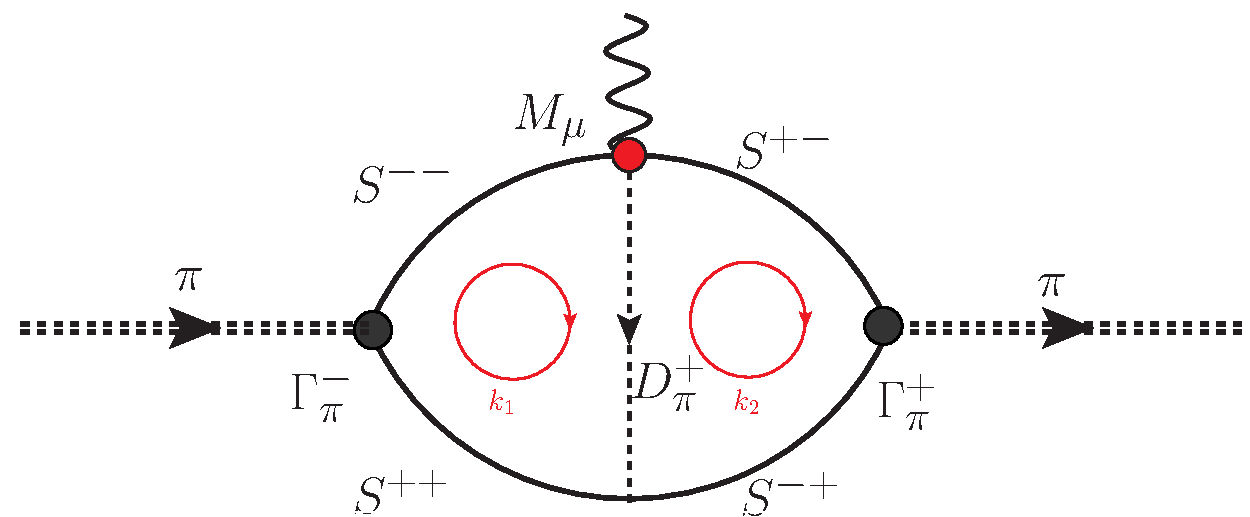
\includegraphics[width=0.7\textwidth]{figures/FF_C}
\caption{\label{fig:FF_C}\footnotesize The third diagram (seagull), which involves the \textit{ansatz} for the quark-pion-photon 4-vertex. All internal vertexes and propagators are dressed.}
\end{figure}
The momenta routing is similar to second diagram and set as following:
\beqa
	&\Gamma_{\pi}^-(k_1,P_-)\;, & S^{--}(k_1 - Q/4 - P/2)\\
	&\Gamma_{\pi}^+(k_2,P_-)\;, & S^{+-}(k_2 + Q/4 - P/2)\\
	&M_{\mu}(\frac{k_1 + k_2 - P}{2})\;, & S^{-+}(k_2 - Q/4 + P/2)\\
	&D_{\pi}^+(Q/2 - k_1 + k_2)\;, & S^{++}(k_1 + Q/4 + P/2)
\eeqa
As well as in previous diagram, $k_1$ and $k_2$ denotes integration momenta, flowing clock-wise as show by red contours on the diagram. $M_{\mu}$ is the \textit{ansatz} for the quark-pion-photon 4-vertex, derived in \cite{s100500070078} and it reads as:
\begin{equation}
\begin{array}{c}
\displaystyle M_\mu(q)=e_q\frac{(4q-Q)_\mu}{4q \cdot Q-Q^2} \left( \chi(q-Q/2) - \chi(q) \right) 
\displaystyle + e_q\frac{(4q+Q)_\mu}{4q \cdot Q+Q^2} \left( \chi(q+Q/2) - \chi(q) \right)
\end{array}
\label{Seagull_vertex}
\end{equation}
where $\chi(q) = S(q+P/2)\Gamma_{\pi}(q,P)S(q-P/2) |_{P^2=M^2}$ and $e_q$ is a quark charge, so the resulting integral reads as:
\begin{equation}
\begin{array}{c}
\displaystyle \frac{P_{\mu}}{P^2} \int\int \frac{d^4k_1}{(2\pi} \frac{d^4k_2}{(2\pi} \Tr \left[  \chi_{\pi}^{+} M_\mu(q) D_{\pi}^{+} \chi_{\pi}^{-} \right] 
\end{array}
\label{Diargam_C}
\end{equation} 
here as well as in previous diagram we denoting $S^{-+}\Gamma_{\pi}^{+}S^{+-} \equiv \chi_{\pi}^{+}$, $S^{--}\Gamma_{\pi}^{-}S^{++} \equiv \chi_{\pi}^{-}$ and $D_{\pi}^{+} = \frac{1}{\frac{Q}{2} - k_1 + k_2 + m_{\pi}^2}$ is pion propagator. Note that there is of course similar diagram, just  mirrored and therefore the quark-pion-photon 4-vertex is $M_{\mu}(\frac{k_1 + k_2 + P}{2})$ and pion propagator is $D_{\pi}^{-} = \frac{1}{-\frac{Q}{2} - k_1 + k_2 + m_{\pi}^2}$.\\

\subsection*{Pion Form Factor}
As we saw in the DSE/BSE approach, pion cloud effects enter in the dynamical properties as a form factor in various ways: starting from solving the quark DSE the pion exchange contributes to dressed quark propagator; through the appropriate two-body kernel the pion cloud impacts on Bethe-Salpeter amplitudes of pion and photon; and finally after kernel gauging procedure the pion cloud exposes itself by producing extra diagrams for the calculation of form factor. 
\begin{figure}[!]
\centering
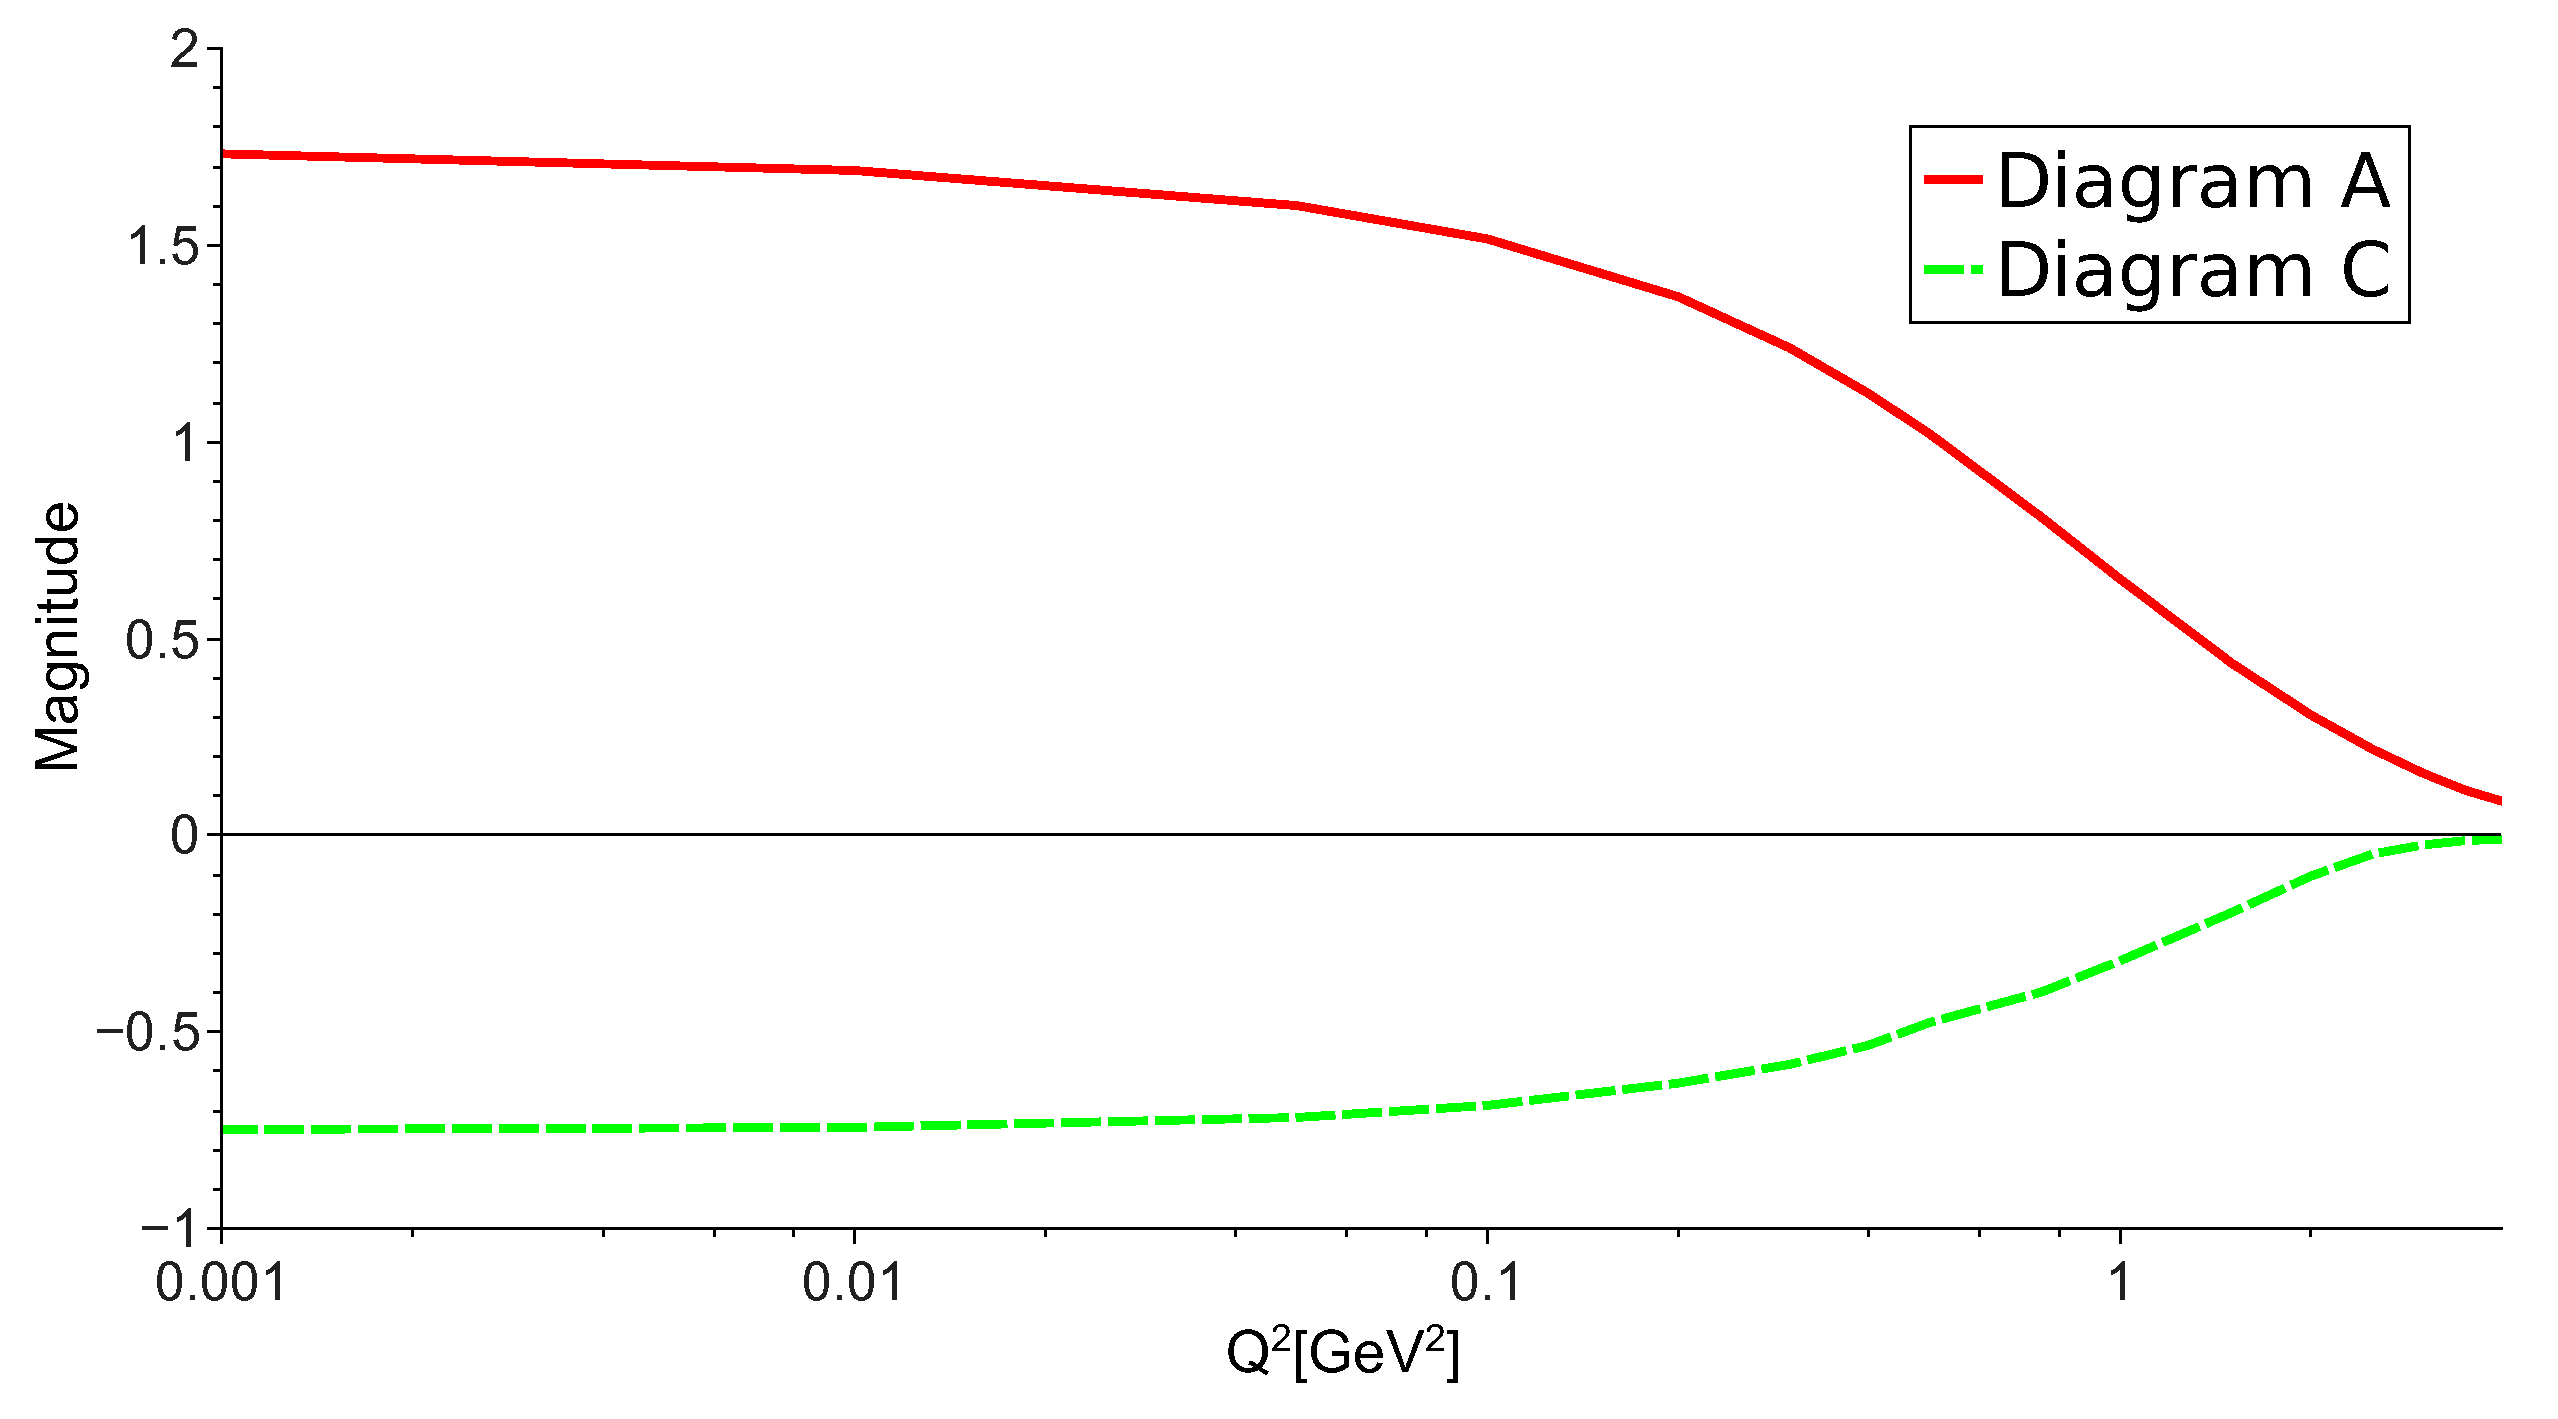
\includegraphics[width=0.99\textwidth]{figures/FF_A_C}
\caption{\label{fig:FF_A_C}\footnotesize The contribution of A and C diagrams for comparison as a function of $Q^2$. Sum of them at $Q^2=0$ equal $F_\pi(Q^2=0) = 1$ fulfilling the Ward-Takahashi identity and conserving the electric charge. The gluon parameters are $\Lambda=0.84$ and $\eta=1.8$.}
\end{figure} \\

Since as it was mentioned the pion cloud piece enters into the calculation recipe on various levels it is crucial to keep under control by tracking the Ward-Takahashi identity and charge conservation. On the form factor level this implies $F_\pi(Q^2=0)=1$. This fact can be easily understood from the qualitative point of view: if we probe the charged pion by very long wave-length photon we will not resolve any internal structure, the point-like charged pion. If the resulting form factor at $Q^2=0$ is $F_\pi(Q^2=0)=1$, then this signal us that the normalization of the BSA was done
correctly and the electric charge is conserved. In case of rainbow-ladder gluon this would require us to calculate only one diagram given on Fig. \ref{fig:FF_RL}, however in case of pion cloud effect all three diagrams on Fig. \ref{fig:FF_with_pi}. Fortunately the second diagram B is zero everywhere on $Q^2$ due to momenta routing specificness, and therefore does not contribute to the form factor. This fact leaves us with two diagrams: A and C, they contribution to pion form factor is shown on Fig. \ref{fig:FF_A_C}.
\begin{figure}[h]
\centering
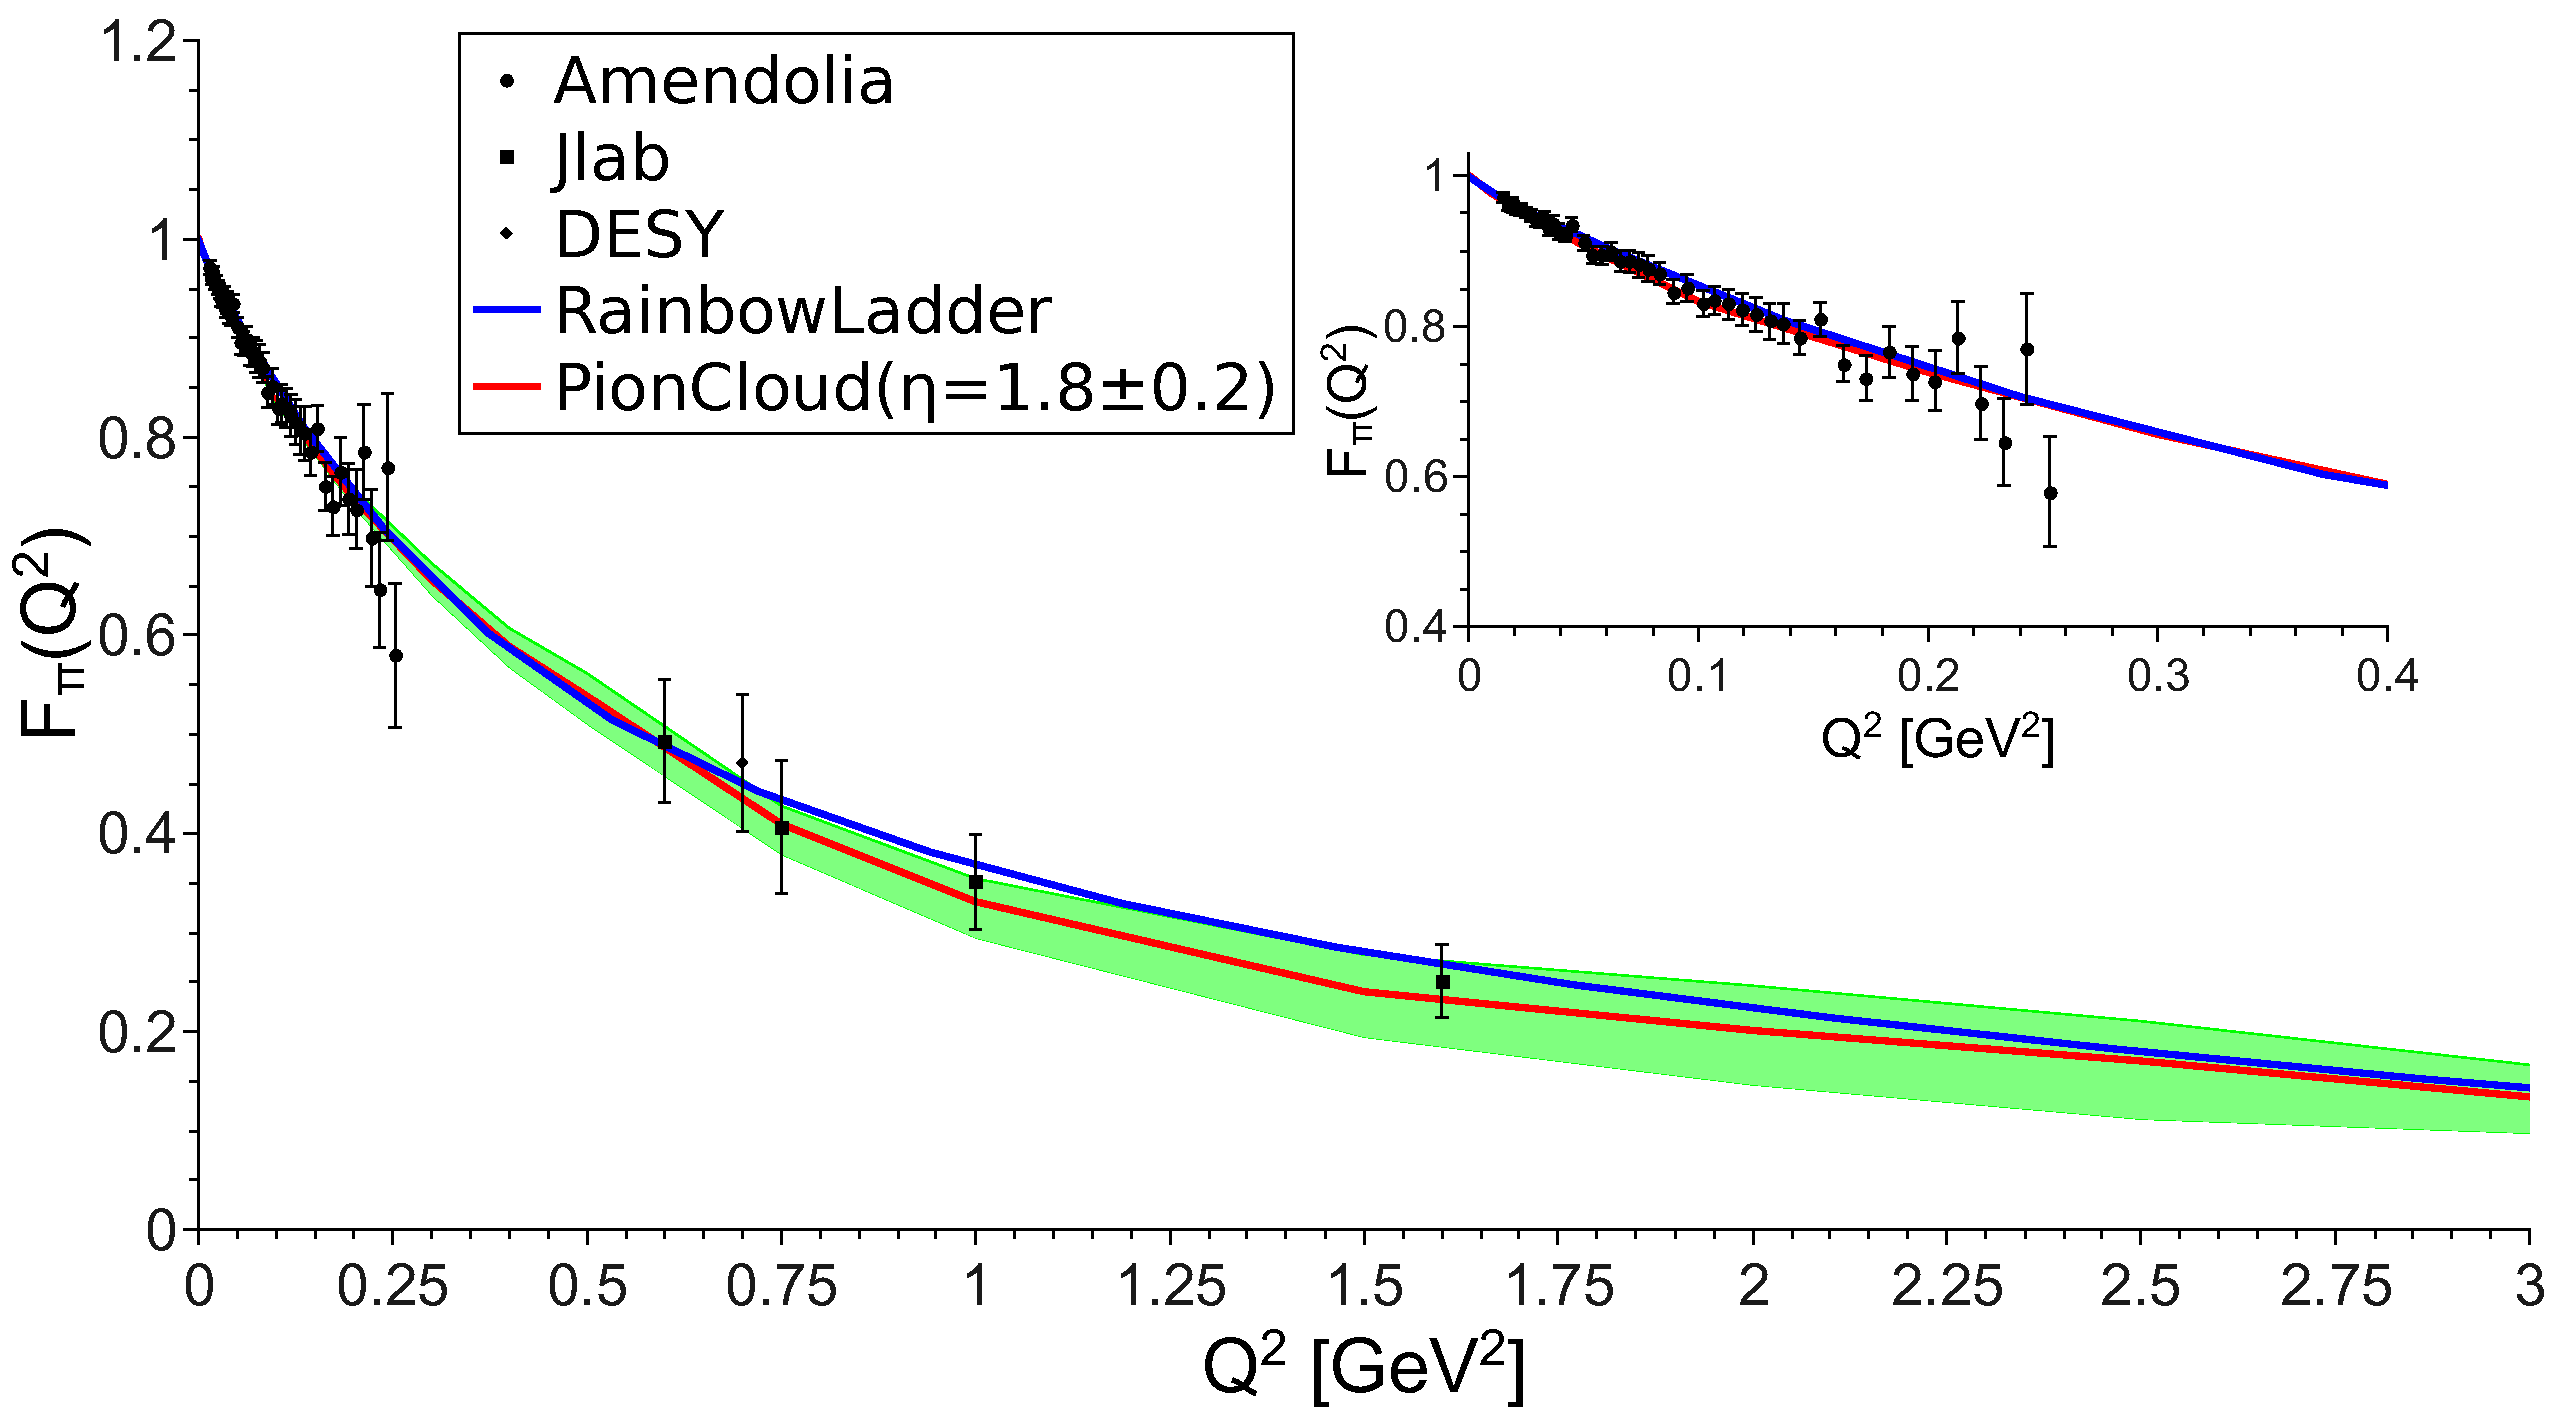
\includegraphics[width=0.99\textwidth]{figures/FF_RL_PS}
\caption{\label{fig:FF_RL_PS}\footnotesize The resulting pion form factor for two types of kernels: blue lines correspond to single rainbow-ladder gluon exchange only; red line to the gluon exchange with pion cloud effect. The green area correspond to $\eta$ parameter variation. The experemental data obtained from \cite{Amendolia:1986wj,Volmer:2000ek}.}
\end{figure} \\

In Fig. \ref{fig:FF_RL_PS} we present numerical results for the pion form factor carried out within two schemes: rainbow-ladder single gluon exchange and pion cloud effect impact. We compare them to available experimental data, obtained within \cite{Amendolia:1986wj,Volmer:2000ek}. Firstly we observe that both of truncations provide the charge conservation and fulfil the Ward-Takahashi identity as the calculated form factor fulfils the condition $F_\pi(Q^2=0)=1$. The interesting discrepancy arises at the intermediate range of $Q^2$. For $0.75\; \text{GeV}^2 < Q^2 < 1.75\; \text{GeV}^2$ the pion form factor with pion cloud deviates from rainbow-ladder result at the level of 10 percents. The qualitative explanation is the following: at very low $Q^2$ photon resolves the pion as a whole thing without any substructure, whether at very large $Q^2$ it resolves the separate quarks and at aforementioned intermediate range of $Q^2$ the photon "sees" the pion quark core and the pion cloud surrounding it. Obviously this does not happen in case if the only gluon exchange taken into account. The observation that the form factor with pion cloud is smaller than rainbow-ladder one reflects the fact that the virtual pions provide the charge screening effect in that kinematic range. Unfortunately, the experimental data in that region does not allow to distinguish between the single gluon exchange and the pion cloud picture due to big error bars. However it is potentially plausible to estimate the pion cloud effect with improved experimental statistics. At the ultraviolet limit both curves tend to merge since the pion cloud effect diagram C fades faster with growing $Q^2$ that diagram A, according to Fig. \ref{fig:FF_A_C}, because of the specifics of momenta routing.





%\chapter{3-body bound states equation}
\label{chap:fadeev}

\section{Fadeev equation}
	\subsection{Notation}
	\subsection{Pion cloud effect}
	\subsection{Nucleon and Delta masses}
\chapter{Summary and outlook}
\label{chap:sum}
\vspace{-1.0cm}
Some of the mysteries of QCD phenomenology can be face with the framework of the coupled quark \DSE, meson \BSE and baryon Faddeev equation, providing non-perturbative, continuum and Poincare invariant scientific approach. The research performed throughout this thesis is twofold. From one perspective we focus on the investigation of mass spectra for mesons with total spin quantum number $J=3$ and arising Regge-trajectory for natural parity states $J^{PC}=1^{--},2^{++},3^{--}$ within rainbow-ladder single gluon exchange model. The other findings are concerning the impact of the pion cloud effect on $J>2$ meson states, baryon masses, namely on Nucleon and Delta three-body bound states and meson dynamical properties like the pion form factor.\\
\vspace{-0.3cm}

For meson mass spectra studies we employ a simple interaction model, the effective gluon rainbow-ladder
approximation, which is known to represent only part of the complicated interaction pattern of quarks and gluons even for heavy quarks. However for the light quarks we obtained quantitatively reliable results for channels where only the contact part of the spin-spin interaction plays a role and channels dominated by the spin-orbit force, {\it i.e.} $J^{PC}= 2^{++}, 3^{--}$. The technical improvement that made available for the calculation mass spectra with quantum numbers $J=3$ allowed us to address the phenomena of Regge mass trajectory within DSE/BSE approach. Despite the fact that the rainbow-ladder approximation has clear deficiencies in the light quark sector we were able to obtain the Regge-trajectory behaviour for natural parity states $J^{PC}=1^{--},2^{++},3^{--}$ deviating from experimental data on the level of 5\%. In the heavy quark sector, where the rainbow-ladder approximation does particularly well, the agreement with the experimental states is much improved. We gave predictions for the tensor charmonia and bottomonia states, in particular for the $3^{--}$. We also gave results for $B_c$ states and quarkonia with exotic quantum numbers, although the accumulated errors in these channels due to deficiencies in the rainbow-ladder interaction may be sizeable.\\
\vspace{-0.3cm}

The another purpose of this thesis is to investigate the impact of the pion cloud effect on Nucleon and Delta three-body bound states masses and pion dynamical properties, specifically the pion electromagnetic form factor. This work complements the efforts in estimating the impact of hadronic unquenching effects, carried out in \cite{Fischer:2007ze,Fischer:2008sp,Fischer:2008wy}. We found substantial contributions of the pion cloud effects to the masses of the baryons of the order of 5-15 \%, depending on the parameters of the underlying quark-gluon interaction.
In addition, we found slight but significant changes in the structure of the baryons reflected in the relative contributions of their partial waves.
Concerning the pion form factor we found a slight deviation from gluon rainbow-ladder results in the range of intermediate momenta transferred, $0.75\; \text{GeV}^2 < Q^2 < 1.75\; \text{GeV}^2$. This deviation reflects the fact that with pion cloud included the pion form factor shows an extra substructure - the virtual pion cloud surrounding the pion quark core. However it is impossible to distinguish these two pictures and estimate the real impact of the pion cloud effect due to lack of experimental data and its accuracy. \\
\vspace{-0.3cm}

The plausible future directions of research would be the calculation of charmonium radiative decays: processes like $J/\psi \rightarrow \gamma \eta_c$, $\chi_{c0} \rightarrow \gamma J/\psi$, and etc. Also it is of the extreme interest is to find a robust way to extract the two-quark (pseudo-) potential out the meson Bethe-Salpeter equations with the given truncation. This can provide a better way to compare the quark potential model approaches to DSE/BSE framework, since this would let us clear understand the impact of the employed truncation on the spin-spin and spin-orbit parts of the two-quark potential. The another direction would be to extend the employed pion cloud framework to baryon form factor calculations.


\begin{appendices}
\chapter{Euclidean space and kinematics}
\label{app:euclidean}
\section*{Metrics}
Lattice QCD and most of nonperturbative quantum field theory approaches are peformed in Euclidead metric for practical reasons. Euclideand 4-vectors can be obtained from the Minkowski 4-vectors via the Wick rotation \cite{PhysRev.96.1124}. Throughout this work we consider the quark \DSE and meson \BSE formulated in Euclidean momentum space. In this case, the metric tensor is given by $g_{\mu\nu}=\delta_{\mu\nu}$. The space-time and momentum-energy vectors are related by:
\beqa
t^E = it^M \\
x^E = x^M \\
E^E = iE^M \\
p^E = p^M \;,
\eeqa
where $E$ and $M$ denote Euclidean and Minkowski space. The Euclidean representation of fundamental hermitian Dirac matrices reads as following:
\beqa
\notag \gamma^1 &=
\begin{pmatrix} 
0 & 0 & 0 & -i \\
0 & 0 & -i & 0 \\ 
0 & i & 0 & 0 \\
i & 0 & 0 & 0 
\end{pmatrix}, \quad
\gamma^2 &= \begin{pmatrix}
0 & 0 & 0 & -1 \\
0 & 0 & 1 & 0 \\
0 & 1 & 0 & 0 \\
-1 & 0 & 0 & 0 \end{pmatrix} \\
\gamma^3 &= \begin{pmatrix}
0 & 0 & -i & 0 \\
0 & 0 & 0 & i \\
i & 0 & 0 & 0 \\
0 & -i & 0 & 0 \end{pmatrix},\quad
\gamma^4 &= \;\;\; \begin{pmatrix}
0 & 0 & 1 & 0 \\
0 & 0 & 0 & 1 \\
1 & 0 & 0 & 0 \\
0 & 1 & 0 & 0 \end{pmatrix}.
\eeqa
In this representation, $\gamma_5=i\gamma_1\gamma_2\gamma_3\gamma_4$ is diagonal. Changing the space also change the product rule and the integration measure: 
\beqa
	\gamma^M \dot p^M &=& -i\gamma^E \dot p^E \\
	q^M \dot p^M &=& - q^E \dot p^E \label{app:shell} \\
	\int d^4 k^M &=& -i \int d^4 k^E
\eeqa
Apparently the definition of the mass shell of the free particle in Euclidean space: $P^2 = -M^2$ follows from Eq.(\ref{app:shell}).

\section*{Kinematics}
It is convenient to write 4-dimensional integration measure in spherical coordinates, so that the explicit form of the momentum integrations reads as:
\beqa
	\int \frac{d^4k}{(2\pi)^4}\; \longrightarrow  \;\frac{1}{(2\pi)^4} \int d(k^2) \frac{k^2}{2} \int_{-1}^1 dz\sqrt{1-z^2} \int_{-1}^1 dy \int_0^{2\pi} d\phi\;,
\eeqa
where the integration momenta $k$ is parametrized as:
\beqa
	k = \sqrt(k^2)\begin{pmatrix} 
 \sqrt{1-z^2}\sqrt{1-y^2}sin(\phi), \\
	\sqrt{1-z^2}\sqrt{1-y^2}cos(\phi), \\
	y\sqrt{1-z^2}, \\
	z 
\end{pmatrix}
	\label{app:momenta_param}
\eeqa
The Eq.(\ref{app:momenta_param}) is the most general parametrization, however in our case due to angle symmetries of quark \DSE and meson \BSE some of the angle integrals are trivial, therefore we can reduce the amount of parameters. As for quark DSE the momenta are given as:
\beqa
	k = \sqrt(k^2)(0,0,0,z)
\eeqa
and for meson BSE we choose total meson momenta $P$ to be in the rest-frame, so $P,p,k$ read as:
\beqa
\notag	P &=& (0,0,0,\sqrt{P^2}) \\
	p &=& \sqrt(p^2)(0,0,\sqrt{1-z_p^2},z_p) \\
\notag	k &=& \sqrt(k^2)(0,\sqrt{1-z^2}\sqrt{1-y^2},y\sqrt{1-z^2},z)
\eeqa
In our study for the numerical calculation we explicitly employed objects like 4d-tensors and gamma matrices provided by QFT++ library \cite{Williams:2008wu}. Note however, that the original QFT++ library uses Minkowski and was rewritten for Euclidean space.





\chapter{Dirac basis of meson BSE}
\label{app:basis}

For the case of $J=1$ we can immediately write down the two rank 1 tensors for a bound state of two
fermions: they are the transversely projected quantities $Q_\mu$ and $T_\mu$ defined 
%
\begin{align}\label{eqn:transverseprojectors}
Q_{\mu} = \tau^{(t)}_{\mu\nu}\; r^\nu\;,\qquad
T_{\mu} = \tau^{(t)}_{\mu\alpha}\; \tau^{(Q)}_{\alpha\nu}\gamma^\nu\;.
\end{align}
%
Here $Q$ is the same quantity as defined in Eq.~\eqref{eqn:transverseQ} and we introduced the 
additional transverse projector $\tau^{(Q)}_{\alpha\nu}$ so that the resulting basis is 
conveniently orthogonal. The explicit components of this basis can be found {\it e.g.} in 
Ref.~\cite{Maris:1999nt}.


%
%
%
%
%
For total angular momentum $J=2$ we construct the $2$-fold tensor products of $Q_{\mu_i}$ and 
$T_{\mu_i}$. Since the product of two or more $T_{\mu_i}$ is degenerate, this gives 
%
\begin{align}
  \tilde{Q}_{\mu_1\mu_2} &= Q_{\mu_1}Q_{\mu_2} \; , \\
  \tilde{T}_{\mu_1\mu_2} &=T_{(\mu_1}Q_{\mu_2)} \;,%+ T_{\mu_2}Q_{\mu_1} \; \; ,
\end{align}
%
where ${(\ldots)}$ denotes the symmetrization of the indices without normalization 
$\nicefrac{1}{J!}$.
%
To satisfy the criteria of being angular momentum tensors we then subtract the trace-part to give~\cite{LlewellynSmith:1969az,Krassnigg:2010mh}
%
\begin{align}
  Q_{\mu_1\mu_2} &= Q_{\mu_1} Q_{\mu_2} - \frac{1}{3}Q^2 \tau_{\mu_1\mu_2} \;, \\
  T_{\mu_1\mu_2} &= T_{(\mu_1} Q_{\mu_2)} -\frac{2}{3} \Sla{Q}\tau_{\mu_1\mu_2}\;.
    %Q_{\mu_1\mu_2} &= \tilde{Q}_{\mu_1\mu_2} - \frac{1}{3}\tau_{\mu_1\mu_2}\tilde{Q}^{\kappa}_{\phantom{\kappa}\kappa} \nonumber \\
  %&= Q_{\mu_1} Q_{\mu_2} - \frac{1}{3}Q^2 \tau_{\mu_1\mu_2} \;, \\
  %T_{\mu_1\mu_2} &= \tilde{T}_{\mu_1\mu_2} - \frac{1}{3}\tau_{\mu_1\mu_2}\tilde{T}^{\kappa}_{\phantom{\kappa}\kappa} \nonumber \\
  %&= T_{(\mu_1} Q_{\mu_2)} -\frac{2}{3} \Sla{Q}\tau_{\mu_1\mu_2}\;.
\end{align}
The explicit components of this basis can be found {\it e.g.} in Ref.~\cite{Krassnigg:2010mh}.
%
%
For total angular momentum $J=3$ we construct the $3$-fold tensor products of $Q_{\mu_i}$ and 
$T_{\mu_i}$
%
\begin{align}
  \tilde{Q}_{\mu_1\mu_2\mu_3} &= Q_{\mu_1}Q_{\mu_2}Q_{\mu_3} \; , \\
  \tilde{T}_{\mu_1\mu_2\mu_3} &= T_{(\mu_1}Q_{\mu_2}Q_{\mu_3)}\;.
\end{align}
%
To satisfy the requirements of angular momentum tensors we subtract the trace part, yielding
%
\begin{align}
  Q_{\mu_1\mu_2\mu_3} &= \tilde{Q}_{\mu_1\mu_2\mu_3} - \frac{1}{5} 
   \tau_{(\mu_1\mu_2}\tilde{Q}^{\kappa\kappa}_{\phantom{\kappa\kappa}\mu_3)}  \;\; , \nonumber\\
  &= Q_{\mu_1}Q_{\mu_2}Q_{\mu_3} - \frac{ 1 }{5}Q^2 
   \tau_{(\mu_1\mu_2} Q_{\mu_3)} \; \;, \\
  T_{\mu_1\mu_2\mu_3} &=\tilde{T}_{\mu_1\mu_2\mu_3} -\frac{1}{5} 
   \tau_{(\mu_1\mu_2}\tilde{T}^{\kappa\kappa}_{\phantom{\kappa\kappa}\mu_3)}  \nonumber \\
  &= T_{(\mu_1}Q_{\mu_2} Q_{\mu_3)} - \frac{1}{5} 
   2\Sla{Q}\tau_{(\mu_1\mu_2}Q_{\mu_3)}  \nonumber \\
   & - \frac{1}{5} Q^2\tau_{(\mu_1\mu_2} T_{\mu_3)}   \;,
\end{align}
%
which has not been explored in this approach before. The explicit representation of this basis is given by
%
\begin{align}
%
\Gamma^{(\ONE)}_{\mu_1\mu_2\mu_3}(r,t) &= 
   Q_{\mu_1\mu_2\mu_3} \left[ \lambda_1 \ONE + \lambda_2\slashed{t} +\lambda_3 \slashed{Q} + \lambda_4\slashed{Q}\slashed{t}  \right]\nonumber\\
 &+T_{\mu_1\mu_2\mu_3}\; \left[ \lambda_5 \ONE + \lambda_6\slashed{t} +\lambda_7 \slashed{Q} + \lambda_8\slashed{Q}\slashed{t}  \right]\;,
%
\end{align}
with $\lambda_i=\lambda_i(r,t)$ scalar coefficients. Multiplying through by $\gamma_5$ would yield the 
$\Gamma^{(5)}_{\mu_1\mu_2\mu_3}(r,t)$ basis decomposition. \\

The quantum numbers of a meson in the non-relativistic quark model are obtained from the spin, $S$, 
and relative orbital angular momentum $L$ of the $q\bar{q}$ system, which combine to give the total 
spin $J=L\oplus S$. The total parity, $P$, charge parity, $C$, and $G$ parity are given by
%
\begin{align}
P\left(q\bar{q}\right) &= -(-1)^{L}\;, \\
C\left(q\bar{q}\right) &= \phantom{-}(-1)^{L+S}\;, \\
G\left(q\bar{q}\right) &=\phantom{-}(-1)^{L+S+I}\;,  
\end{align}
%
where $C$ parity only applies to charge neutral states and is generalized to $G$ parity for isospin $I=1$.\\

Thus, the quark model yields the possible $J^{PC}$ quantum numbers in Table~\ref{tab:qmodel}.
%
This leaves us with five states (for $J\le3$) that are considered exotic:
$J^{PC} = 0^{--}$, $J^{PC} = 0^{+-}$, $J^{PC} = 1^{-+}$, $J^{PC} = 2^{+-}$,  and $J^{PC} = 3^{-+}$.
%
\begin{table}[!h]
\renewcommand{\arraystretch}{1.3}
\begin{tabular*}{\columnwidth}{@{\extracolsep{\stretch{1}}}lll|lll|lll|lll|lll@{}}
\hline
\hline
L & S & $J^{PC}$ & L & S & $J^{PC}$ & L & S & $J^{PC}$ & L & S & $J^{PC}$ & L & S & $J^{PC}$ \\
\hline
0 & 0 & $0^{-+}$ & 1 & 0 & $1^{+-}$ & 2 & 0 & $2^{-+}$ & 3 & 0 & $3^{+-}$ & 4 & 0 & $4^{-+}$ \\
0 & 1 & $1^{--}$ & 1 & 1 & $0^{++}$ & 2 & 1 & $1^{--}$ & 3 & 1 & $2^{++}$ & 4 & 1 & $3^{--}$ \\
  &   &          & 1 & 1 & $1^{++}$ & 2 & 1 & $2^{--}$ & 3 & 1 & $3^{++}$ & 4 & 1 & $4^{--}$ \\
  &   &          & 1 & 1 & $2^{++}$ & 2 & 1 & $3^{--}$ & 3 & 1 & $4^{++}$ & 4 & 1 & $5^{--}$ \\  

\hline
\hline
\end{tabular*}
\caption{Allowed quantum numbers for a neutral $q\bar{q}$ state in the quark model. \label{tab:qmodel}}
\end{table}
\chapter{Numerical methods}
\label{app:numerics}

\section*{Integration}
\subsection*{Gauss quadratures}
In order to perform numerical integration we discretise radial and two angles integrals into a quadrature sums \cite{Press:2007:NRE:1403886} as follows:
\beqa
\int d(k^2) \frac{k^2}{2} \int_{-1}^1 dz\sqrt{1-z^2} \int_{-1}^1 dy \longrightarrow \sum^{N_k}_{n=1} \sum^{N_z}_{m=1} \sum^{N_y}_{l=1} w(k_n) w(z_m) w(y_l)\;,
\eeqa
where $w(k_n), w(z_m), w(y_l)$ are quadrature weights and $k_n, z_m, y_l$ are correspondent nodes. The integral over $\phi$ is not considered here since it is for our calculation it is trivial and equal $2\pi$. The radial and $y$-angle integrations involve a trivial integration measure therefore for them we employ Gauss-Legendre quadrature. In case of $z$-angle we need to incorporate the factor $\sqrt{1-z^2}$ into quadrature rule to archive a good accuracy. The proper way to do so is to apply Gauss-Chebyshev quadrature by expanding the integral into following form:
\beqa
	\int_{-1}^1 dz\sqrt{1-z^2} f(z)  \longrightarrow \sum^{N_z}_{m=1} w(z_m) f(z_m)\;,
\eeqa
here nodes are $z_m=cos(\frac{m}{N_z+1}\pi)$ and weights are $w_m=\frac{\pi}{N_z+1}sin^2(\frac{m}{N_z+1}\pi)$. 
%
\subsection*{Cauchy integration}
\begin{figure}[!b]
\begin{center}
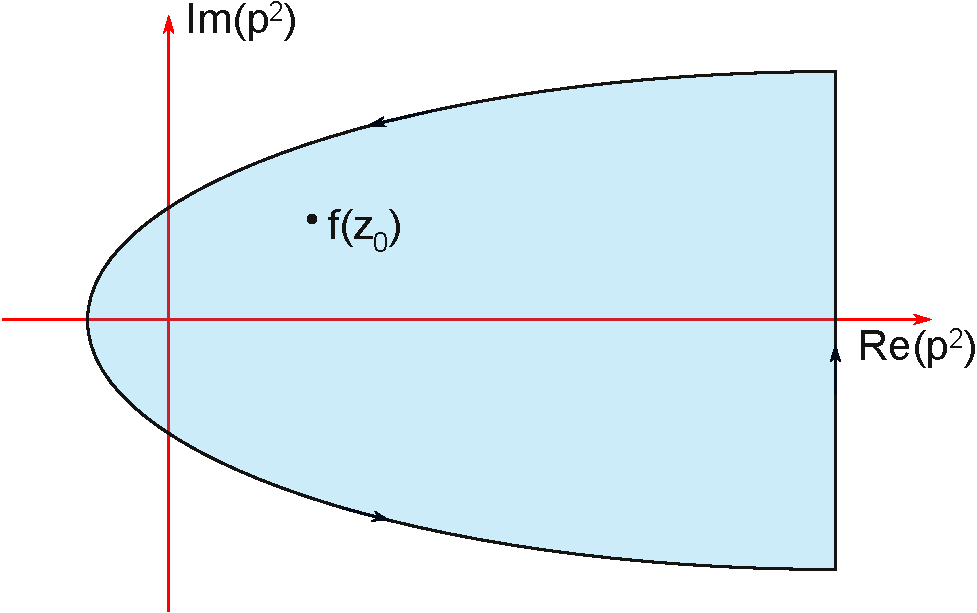
\includegraphics[width=0.8\columnwidth]{figures/contour}
\caption{Sketch of the integration contour for the determination of the quark propagator in
the complex plane.}\label{fig:contour1}
\end{center}
\end{figure}
%
In the BSE due to the external total momentum of the bound state one needs to evaluate the
internal propagators on the right hand side in a parabola region given by Eq.(\ref{dse:contour}) and sketched in Fig.~\ref{fig:contour1}.
Recall that parabolic $p^2$-contour in complex momentum region is parametrizes as follows:
\beqa
	p^2 = t^2 + itM_{state} - \frac{M_{state}^2}{4}\;,
	\label{dse:app_contour}
\eeqa
where the parameter $t$ in given by Gauss quadrature notes $k_n$.
The DSE is then solved iteratively on the boundary supplemented
with Cauchy's theorem, which reads as: given a function $f(z)$ defined on the 
boundary of a closed contour $z\in\mathcal{C}$, we have for any $z_0$ inside:
%
\begin{align}\label{eqn:cauchy}
f(z_0) = \frac{1}{2\pi i} \oint_{\mathcal{C}} \frac{dz f(z)}{z-z_0}\simeq \frac{1}{2\pi i} \sum_{i} \frac{w_i f(z_i)}{z_i-z_0}\;,
\end{align}
%
where the integral has been approximated by some quadrature formula with weights $w_j$ and 
abscissa $z_j$. This is paired with a parametric mapping that describes the contour's boundary.
Numerically this procedure poses a challenge when $z_0$ approaches the abscissa $z_i$. This can be 
mitigated through the use of the barycentric formula~\cite{Berrut_barycentriclagrange}
%
\begin{align}\label{eqn:cauchybary}
f(z_0) = \frac{\sum_{i} \bar{w}_i f(z_i)  }{\sum_{i} \bar{w}_i }\;,\;\;\;\;\bar{w}_i=w_i /\left(z_i-z_0\right)\;
\end{align}
%
%
With this improvement applied, when when $z_0$ approaches the abscissa $z_i$ and the nominator diverges the same happens in denominator so the divergences cancel up to first order error. 

\section*{Power method}
The basic idea is to start with initial guess for the solution and then to generate iterative series converging to the final solution. The scheme can be represented by Eq. \ref{app:solution_scheme}:
\beqa
\label{app:solution_scheme}
F^{(1)}(p) = K(k,p,...) \otimes F^{\text{initial guess}}(k) \\ 
F^{(2)}(p) = K(k,p,...) \otimes F^{(1)}(k) \\ 
\notag &...& \\
F^{(n)}(p) = K(k,p,...) \otimes F^{(n-1)}(k)
\eeqa
Here a number in brackets denote an iteration step, the $K(k,p,...)$ schematically represents the appropriate quark-quark scattering kernel for quark DSE or meson BSE. The sign $\otimes$ represent the the Dirac trace and integration. In this case the sampling of the internal grid $(k)$ can be set similar to external grid $(p)$. Note that the quark DSE takes as input the quark propagator $S(k)$, but outputs inverted one $S^{-1}(p)$. The iterations must be performed until they converged to solution at desired accuracy level.  \\ 

In case of shifted momenta, as it was considered in \ref{chap:BSE}, this robust method cannot be applied due to non-trivial momenta routing:
\beqa
F(p) = K_{\text{shifted}}(k,p,...) \otimes F(p-k)\;, 
\label{app:solution_scheme_shift1}
\eeqa
where a notion $\text{shifted}$ reflects the fact that the scattering kernel also changes due to the momenta shifting. From Eq.(\ref{app:solution_scheme_shift1}) it is clear, that the internal grid $(p-k)$ does not match to external $(p)$ and moreover the internal grid depends on external. The additional complexity comes from the fact that in case of quark DSE the propagator, meant to be used in meson BSE later, has to be obtained within parabolic region in complex plane defined by:
\beqa
	p^2 = t^2 + itM_{meson} - \frac{M_{meson}^2}{4} 
	\label{app:contour}
\eeqa
The following external grid $(p^2)$ and internal grid $(p-k)^2$ are shown on Fig. \ref{fig:contour2}. 
\begin{figure}[h]
\begin{center}
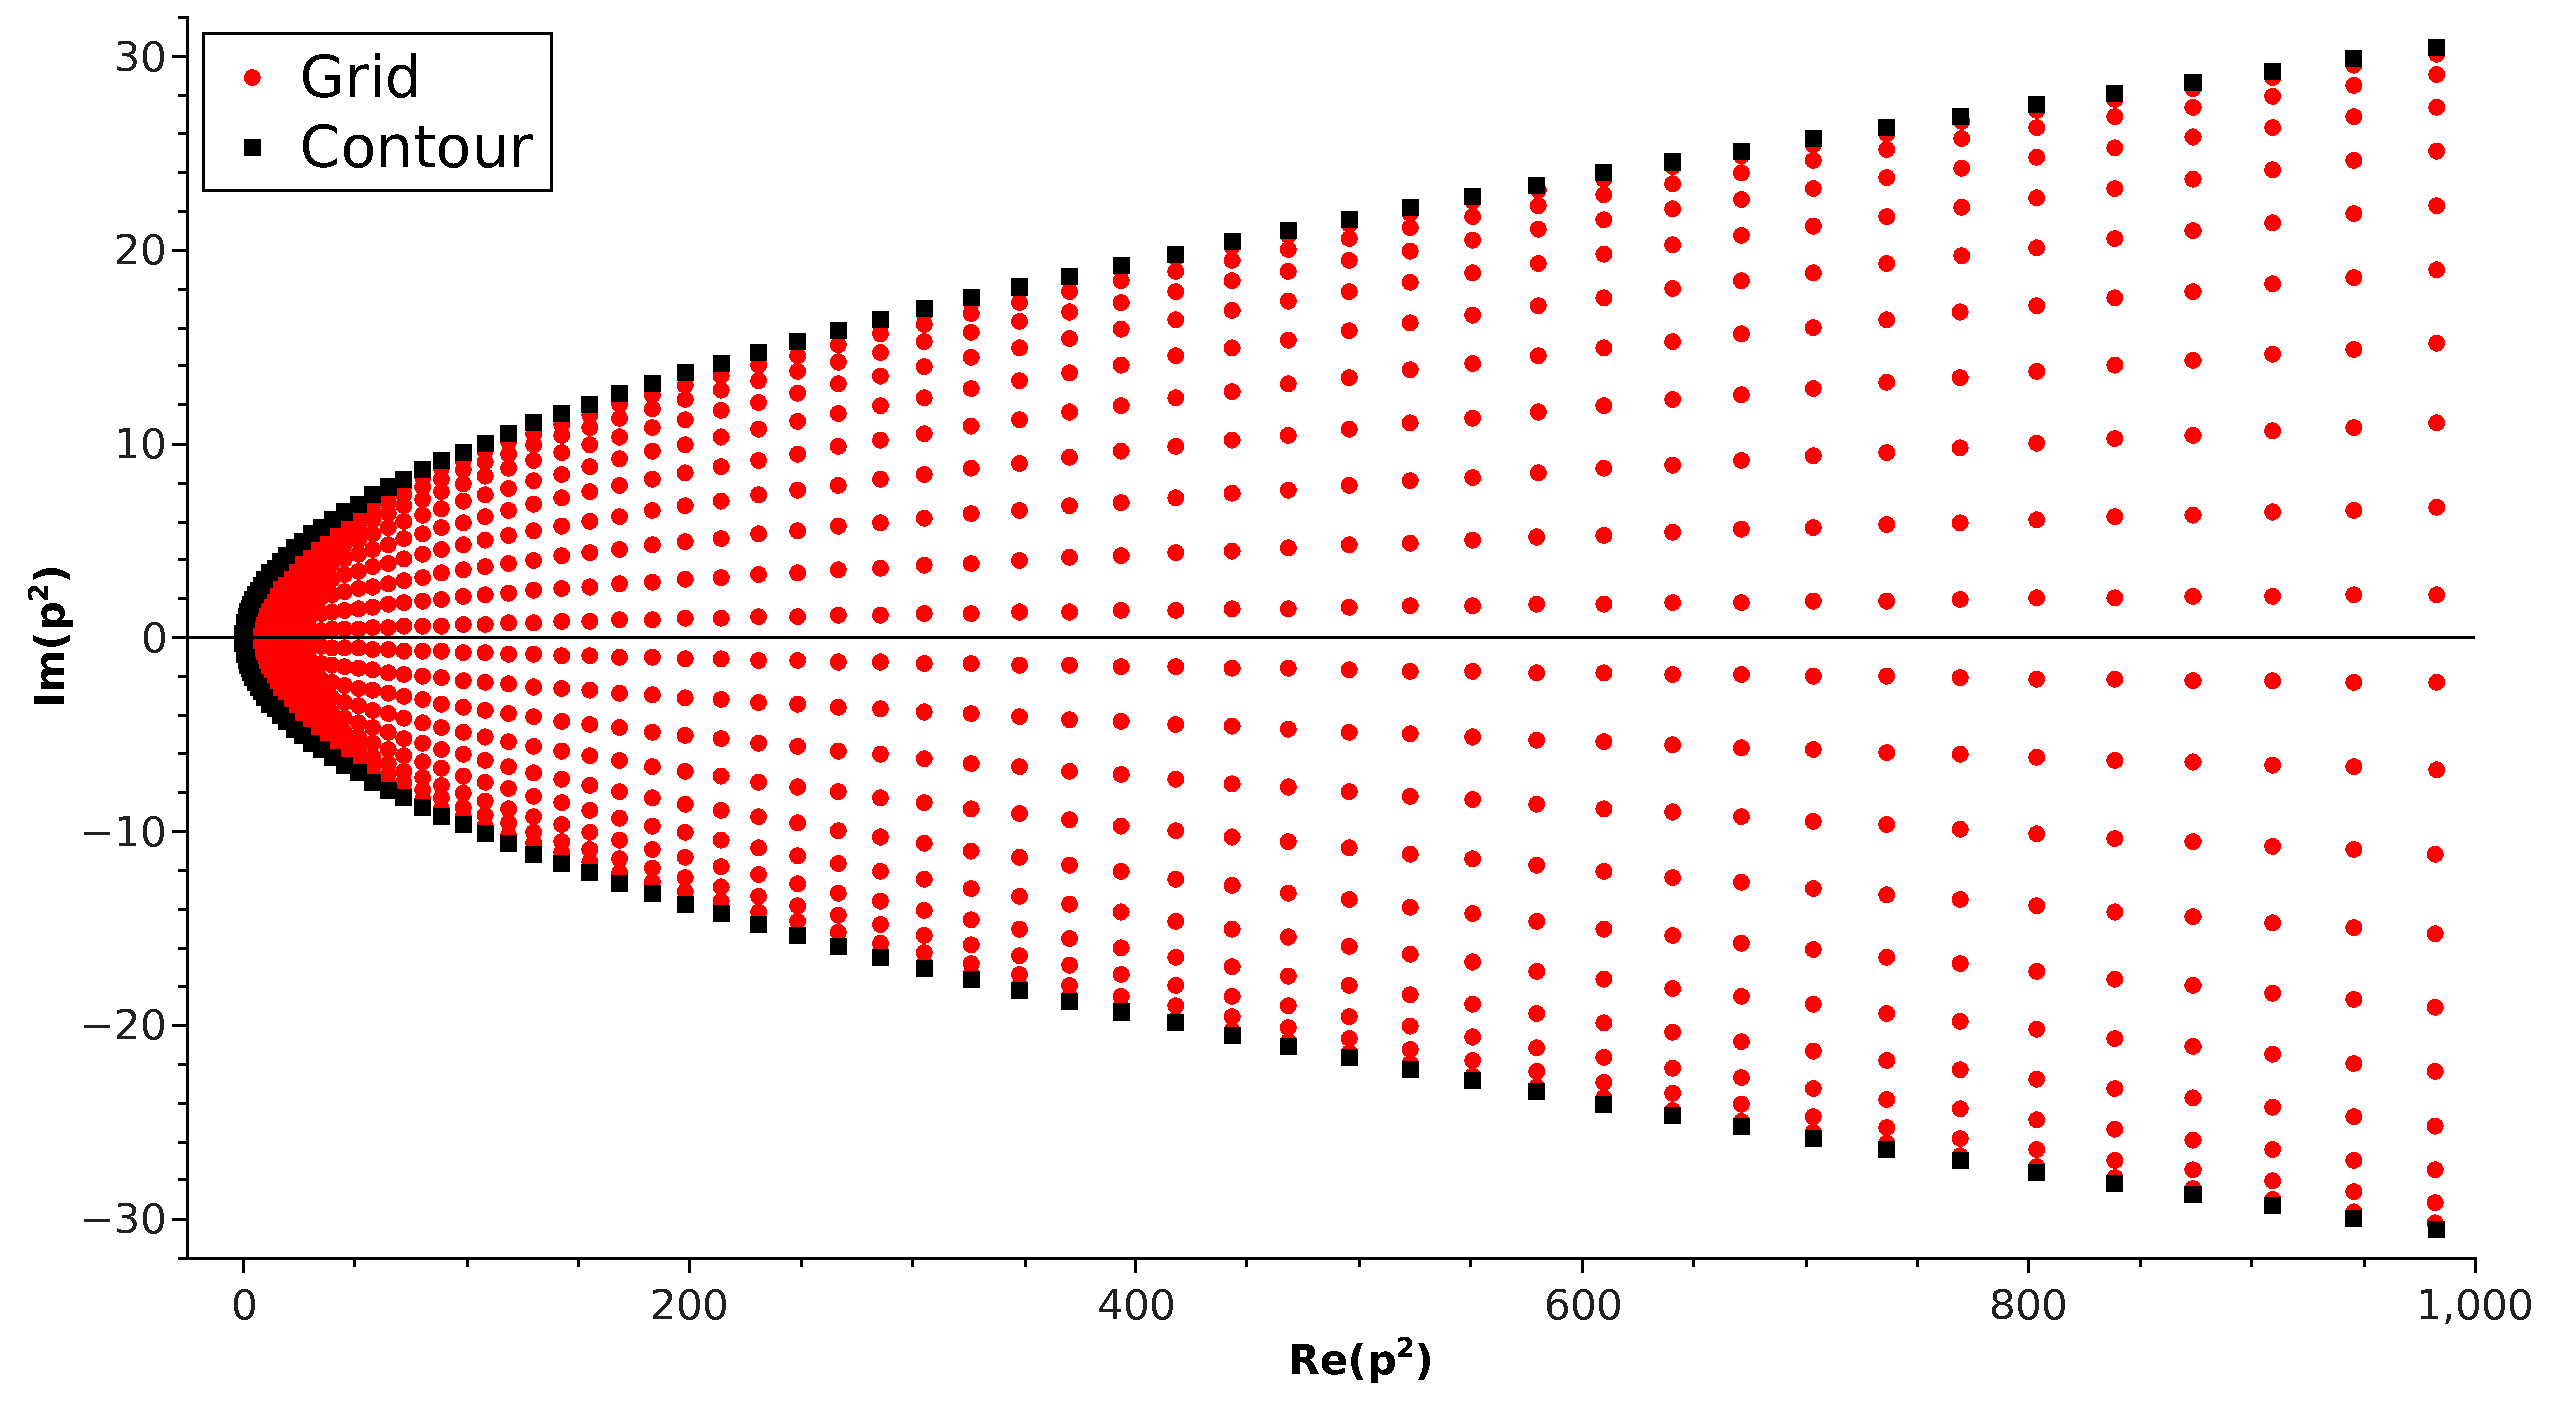
\includegraphics[width=0.99\textwidth]{figures/Grid_to_Contour}
\caption{\footnotesize }\label{fig:contour2}
\end{center}
\end{figure}
However the two observations can be made: every point of the internal grid $(p-k)^2$ for any $k$ lies within parabolic region $(p^2)$; the dressing functions posses analyticity property and therefore if they are known on a contour, using the Cauchy theorem we can obtain them everywhere inside a contour. In order to employ this idea we need to truncate our parabolic region at $\Lambda$ UV scale and by that turn it into the contour, where $\Lambda$ is same as the upper limit of a loop integration. The power method in this case has one extra step:
\beqa
\label{app:solution_scheme_shift2}
F^{(1)}(p) = K_{\text{shifted}}(k,p,...) \otimes F^{\text{initial guess}}(p-k) \\
F^{(1)}(p-k) = \mathfrak{C} \left(  F^{(1)}(p) \right)  \\ 
F^{(2)}(p) = K_{\text{shifted}}(k,p,...) \otimes F^{(1)}(p-k) \\
\notag &...& \\
F^{(n)}(p) = K_{\text{shifted}}(k,p,...) \otimes F^{(n-1)}(p-k)\;,
\eeqa
here $\mathfrak{C}$ denotes the mapping from external grid $(p^2)$ to internal grid $(p-k)^2$ via the Cauchy integral. The Eq.(\ref{app:solution_scheme_shift2}) is written in a general notation to stress the fact that this approach can be applied to both quark DSE and homogeneous/inhomogeneous meson BSE. The power methods have a major drawback - one can obtain only the first dominant solution and in case of meson BSE this would mean it would obtain only the ground state. 

\section*{Matrix eigenvalue calculation}
The meson \BSE can be considered as eigenvalue problem, such that the Eq.(\ref{bse:BSE_gen}), given by:
\beqa
	\Gamma^{(\mu...)}_{tu}(p;P) = \lambda(P^2) \int \frac{d^4 k}{(2\pi)^4} K_{tu;rs}(p,k;P)\left[ S(k_+)\Gamma^{(\mu...)}(k;P)S(k_-)\right]_{sr}\;,
	\label{app:BSE_gen}
\eeqa
after transforming the integration into Gaussian quadrature \cite{Press:2007:NRE:1403886} according to Appendix \ref{app:euclidean}, the meson BSE can be written as:
\beqa
	\mathcal{A}_i = \lambda(P^2) \mathcal{K}_{ik} \mathcal{A}_k\;,
\eeqa
where the index $i$ at $A$ denotes not only the appropriate scalar \BS amplitude but also the quadrature integration point, so the vector $A_i$ takes the following form:
\beqa
\mathcal{A} =
	\begin{pmatrix} 
A_1(p^2_{(1)},z_{(1)},P^2) \\
A_1(p^2_{(2)},z_{(1)},P^2) \\
... \\
A_1(p^2_{(1)},z_(2),P^2) \\
... \\
A_2(p^2_{(1)},z_{(1)},P^2) \\
...
\end{pmatrix},
\eeqa
and the matrix $\mathcal{K}_{ik}$ consists of traces of the angular tensor in $\Gamma^{(\mu...)}_{tu}(p;P)$ from r.h.s in Eq.(\ref{bse:BSE_gen}), the scattering kernel $K_{tu;rs}(p,k;P)$, two propagators $S(k_+),S(k_-)$ and the the angular tensor in $\Gamma^{(\mu...)}(k;P)$ from l.h.s, so the matrix $\mathcal{K}_{ik}$ reads as:
\beqa
Tr \left[  D^{(i)}_{r}(p^2_{(i)},z_{r(i)}) K(p^2_{(i)},z_{r(i)},k^2_{(k)},z_{l(k)})  S_+(k^2_{(k)}) D^{(k)}_{l}(k^2_{(k)},z_{l(k)}) S_-(k^2_{(k)}) \right],
\eeqa
where $D_{r}(p;P)$ and $D_{l}(k;P)$ are the angular tensors from r.h.s and l.h.s respectively and for a brevity we omitted $P$ dependence. In simple words the index $i$ denotes iteration over amplitude projector $D_{r}$ and over $(p^2,z_r)$ external grid points, whether index $k$ denotes amplitude projector $D_{r}$ and $(k^2,z_l)$ internal grid points. Once the matrix $\mathcal{K}_{ik}$ in allocated on the required external $(p^2,z_r)$ and internal $(k^2,z_l)$ grids for all amplitudes for the desired $J^{PC}$ we can employ the numerical eigenvalue calculation routine, namely the eigenvalue decomposition. The numerical routine is provided by the \emph{Eigen} library~\cite{eigenweb}. We specify the $J^P$ of the state through the choice of the covariant decomposition, section~\ref{bse:angular_tensor}, and determine the $C$-parity of the state by examining the symmetry properties of the eigenvector. \\
\end{appendices}
%\chapter{Electromagnetic properties of mesons}
\label{chap:EM_props}

\section{Pion form factor}
	\subsection{Rainbow-Ladder approach}
	\subsection{Pion exchange effect}
\section{Electromagnetic properties of charm bound states}
	\subsection{Elastic and transitional form factors}
	\subsection{Radiative decays}

%-----------------------------------------------------------------------------
%\backmatter
\addcontentsline{toc}{chapter}{Bibliography}
\bibliographystyle{h-physrev} 
\bibliography{thesis}

\end{document}
